% Options for packages loaded elsewhere
\PassOptionsToPackage{unicode}{hyperref}
\PassOptionsToPackage{hyphens}{url}
\PassOptionsToPackage{dvipsnames,svgnames,x11names}{xcolor}
%
\documentclass[
  letterpaper,
  DIV=11,
  numbers=noendperiod]{scrreprt}

\usepackage{amsmath,amssymb}
\usepackage{iftex}
\ifPDFTeX
  \usepackage[T1]{fontenc}
  \usepackage[utf8]{inputenc}
  \usepackage{textcomp} % provide euro and other symbols
\else % if luatex or xetex
  \usepackage{unicode-math}
  \defaultfontfeatures{Scale=MatchLowercase}
  \defaultfontfeatures[\rmfamily]{Ligatures=TeX,Scale=1}
\fi
\usepackage{lmodern}
\ifPDFTeX\else  
    % xetex/luatex font selection
\fi
% Use upquote if available, for straight quotes in verbatim environments
\IfFileExists{upquote.sty}{\usepackage{upquote}}{}
\IfFileExists{microtype.sty}{% use microtype if available
  \usepackage[]{microtype}
  \UseMicrotypeSet[protrusion]{basicmath} % disable protrusion for tt fonts
}{}
\makeatletter
\@ifundefined{KOMAClassName}{% if non-KOMA class
  \IfFileExists{parskip.sty}{%
    \usepackage{parskip}
  }{% else
    \setlength{\parindent}{0pt}
    \setlength{\parskip}{6pt plus 2pt minus 1pt}}
}{% if KOMA class
  \KOMAoptions{parskip=half}}
\makeatother
\usepackage{xcolor}
\setlength{\emergencystretch}{3em} % prevent overfull lines
\setcounter{secnumdepth}{5}
% Make \paragraph and \subparagraph free-standing
\makeatletter
\ifx\paragraph\undefined\else
  \let\oldparagraph\paragraph
  \renewcommand{\paragraph}{
    \@ifstar
      \xxxParagraphStar
      \xxxParagraphNoStar
  }
  \newcommand{\xxxParagraphStar}[1]{\oldparagraph*{#1}\mbox{}}
  \newcommand{\xxxParagraphNoStar}[1]{\oldparagraph{#1}\mbox{}}
\fi
\ifx\subparagraph\undefined\else
  \let\oldsubparagraph\subparagraph
  \renewcommand{\subparagraph}{
    \@ifstar
      \xxxSubParagraphStar
      \xxxSubParagraphNoStar
  }
  \newcommand{\xxxSubParagraphStar}[1]{\oldsubparagraph*{#1}\mbox{}}
  \newcommand{\xxxSubParagraphNoStar}[1]{\oldsubparagraph{#1}\mbox{}}
\fi
\makeatother

\usepackage{color}
\usepackage{fancyvrb}
\newcommand{\VerbBar}{|}
\newcommand{\VERB}{\Verb[commandchars=\\\{\}]}
\DefineVerbatimEnvironment{Highlighting}{Verbatim}{commandchars=\\\{\}}
% Add ',fontsize=\small' for more characters per line
\usepackage{framed}
\definecolor{shadecolor}{RGB}{241,243,245}
\newenvironment{Shaded}{\begin{snugshade}}{\end{snugshade}}
\newcommand{\AlertTok}[1]{\textcolor[rgb]{0.68,0.00,0.00}{#1}}
\newcommand{\AnnotationTok}[1]{\textcolor[rgb]{0.37,0.37,0.37}{#1}}
\newcommand{\AttributeTok}[1]{\textcolor[rgb]{0.40,0.45,0.13}{#1}}
\newcommand{\BaseNTok}[1]{\textcolor[rgb]{0.68,0.00,0.00}{#1}}
\newcommand{\BuiltInTok}[1]{\textcolor[rgb]{0.00,0.23,0.31}{#1}}
\newcommand{\CharTok}[1]{\textcolor[rgb]{0.13,0.47,0.30}{#1}}
\newcommand{\CommentTok}[1]{\textcolor[rgb]{0.37,0.37,0.37}{#1}}
\newcommand{\CommentVarTok}[1]{\textcolor[rgb]{0.37,0.37,0.37}{\textit{#1}}}
\newcommand{\ConstantTok}[1]{\textcolor[rgb]{0.56,0.35,0.01}{#1}}
\newcommand{\ControlFlowTok}[1]{\textcolor[rgb]{0.00,0.23,0.31}{\textbf{#1}}}
\newcommand{\DataTypeTok}[1]{\textcolor[rgb]{0.68,0.00,0.00}{#1}}
\newcommand{\DecValTok}[1]{\textcolor[rgb]{0.68,0.00,0.00}{#1}}
\newcommand{\DocumentationTok}[1]{\textcolor[rgb]{0.37,0.37,0.37}{\textit{#1}}}
\newcommand{\ErrorTok}[1]{\textcolor[rgb]{0.68,0.00,0.00}{#1}}
\newcommand{\ExtensionTok}[1]{\textcolor[rgb]{0.00,0.23,0.31}{#1}}
\newcommand{\FloatTok}[1]{\textcolor[rgb]{0.68,0.00,0.00}{#1}}
\newcommand{\FunctionTok}[1]{\textcolor[rgb]{0.28,0.35,0.67}{#1}}
\newcommand{\ImportTok}[1]{\textcolor[rgb]{0.00,0.46,0.62}{#1}}
\newcommand{\InformationTok}[1]{\textcolor[rgb]{0.37,0.37,0.37}{#1}}
\newcommand{\KeywordTok}[1]{\textcolor[rgb]{0.00,0.23,0.31}{\textbf{#1}}}
\newcommand{\NormalTok}[1]{\textcolor[rgb]{0.00,0.23,0.31}{#1}}
\newcommand{\OperatorTok}[1]{\textcolor[rgb]{0.37,0.37,0.37}{#1}}
\newcommand{\OtherTok}[1]{\textcolor[rgb]{0.00,0.23,0.31}{#1}}
\newcommand{\PreprocessorTok}[1]{\textcolor[rgb]{0.68,0.00,0.00}{#1}}
\newcommand{\RegionMarkerTok}[1]{\textcolor[rgb]{0.00,0.23,0.31}{#1}}
\newcommand{\SpecialCharTok}[1]{\textcolor[rgb]{0.37,0.37,0.37}{#1}}
\newcommand{\SpecialStringTok}[1]{\textcolor[rgb]{0.13,0.47,0.30}{#1}}
\newcommand{\StringTok}[1]{\textcolor[rgb]{0.13,0.47,0.30}{#1}}
\newcommand{\VariableTok}[1]{\textcolor[rgb]{0.07,0.07,0.07}{#1}}
\newcommand{\VerbatimStringTok}[1]{\textcolor[rgb]{0.13,0.47,0.30}{#1}}
\newcommand{\WarningTok}[1]{\textcolor[rgb]{0.37,0.37,0.37}{\textit{#1}}}

\providecommand{\tightlist}{%
  \setlength{\itemsep}{0pt}\setlength{\parskip}{0pt}}\usepackage{longtable,booktabs,array}
\usepackage{calc} % for calculating minipage widths
% Correct order of tables after \paragraph or \subparagraph
\usepackage{etoolbox}
\makeatletter
\patchcmd\longtable{\par}{\if@noskipsec\mbox{}\fi\par}{}{}
\makeatother
% Allow footnotes in longtable head/foot
\IfFileExists{footnotehyper.sty}{\usepackage{footnotehyper}}{\usepackage{footnote}}
\makesavenoteenv{longtable}
\usepackage{graphicx}
\makeatletter
\newsavebox\pandoc@box
\newcommand*\pandocbounded[1]{% scales image to fit in text height/width
  \sbox\pandoc@box{#1}%
  \Gscale@div\@tempa{\textheight}{\dimexpr\ht\pandoc@box+\dp\pandoc@box\relax}%
  \Gscale@div\@tempb{\linewidth}{\wd\pandoc@box}%
  \ifdim\@tempb\p@<\@tempa\p@\let\@tempa\@tempb\fi% select the smaller of both
  \ifdim\@tempa\p@<\p@\scalebox{\@tempa}{\usebox\pandoc@box}%
  \else\usebox{\pandoc@box}%
  \fi%
}
% Set default figure placement to htbp
\def\fps@figure{htbp}
\makeatother

\KOMAoption{captions}{tableheading}
\makeatletter
\@ifpackageloaded{bookmark}{}{\usepackage{bookmark}}
\makeatother
\makeatletter
\@ifpackageloaded{caption}{}{\usepackage{caption}}
\AtBeginDocument{%
\ifdefined\contentsname
  \renewcommand*\contentsname{Table of contents}
\else
  \newcommand\contentsname{Table of contents}
\fi
\ifdefined\listfigurename
  \renewcommand*\listfigurename{List of Figures}
\else
  \newcommand\listfigurename{List of Figures}
\fi
\ifdefined\listtablename
  \renewcommand*\listtablename{List of Tables}
\else
  \newcommand\listtablename{List of Tables}
\fi
\ifdefined\figurename
  \renewcommand*\figurename{Figure}
\else
  \newcommand\figurename{Figure}
\fi
\ifdefined\tablename
  \renewcommand*\tablename{Table}
\else
  \newcommand\tablename{Table}
\fi
}
\@ifpackageloaded{float}{}{\usepackage{float}}
\floatstyle{ruled}
\@ifundefined{c@chapter}{\newfloat{codelisting}{h}{lop}}{\newfloat{codelisting}{h}{lop}[chapter]}
\floatname{codelisting}{Listing}
\newcommand*\listoflistings{\listof{codelisting}{List of Listings}}
\makeatother
\makeatletter
\makeatother
\makeatletter
\@ifpackageloaded{caption}{}{\usepackage{caption}}
\@ifpackageloaded{subcaption}{}{\usepackage{subcaption}}
\makeatother

\usepackage{bookmark}

\IfFileExists{xurl.sty}{\usepackage{xurl}}{} % add URL line breaks if available
\urlstyle{same} % disable monospaced font for URLs
\hypersetup{
  pdftitle={Fundamentals of Biological Data Analysis},
  pdfauthor={Stefano Allesina and Dmitry Kondrashov},
  colorlinks=true,
  linkcolor={blue},
  filecolor={Maroon},
  citecolor={Blue},
  urlcolor={Blue},
  pdfcreator={LaTeX via pandoc}}


\title{Fundamentals of Biological Data Analysis}
\author{Stefano Allesina and Dmitry Kondrashov}
\date{2026-09-24}

\begin{document}
\maketitle

\renewcommand*\contentsname{Table of contents}
{
\hypersetup{linkcolor=}
\setcounter{tocdepth}{2}
\tableofcontents
}

\bookmarksetup{startatroot}

\chapter*{Organization of the class}\label{organization-of-the-class}
\addcontentsline{toc}{chapter}{Organization of the class}

\markboth{Organization of the class}{Organization of the class}

\section*{Learning goals}\label{learning-goals}
\addcontentsline{toc}{section}{Learning goals}

\markright{Learning goals}

\begin{itemize}
\tightlist
\item
  \texttt{R} tools for visualizing and analyzing data

  \begin{itemize}
  \tightlist
  \item
    exploration of \texttt{tidyverse}
  \item
    \texttt{dplyr}, \texttt{tidyr} and \texttt{readr} for data wrangling
    and organization
  \item
    \texttt{ggplot2} for visualization
  \item
    specific packages and functions for statistical analysis
  \end{itemize}
\item
  Theory to perform statistical inference

  \begin{itemize}
  \tightlist
  \item
    assumptions of different methods
  \item
    hypothesis testing
  \item
    estimation of parameters
  \item
    model building and selection
  \end{itemize}
\item
  Avoiding common errors

  \begin{itemize}
  \tightlist
  \item
    when (not) to use a statistical method
  \item
    sneaky paradoxes
  \item
    phantom effects
  \end{itemize}
\item
  Work on your own data

  \begin{itemize}
  \tightlist
  \item
    analyze data
  \item
    produce graphics
  \item
    write up a report
  \item
    present to class
  \end{itemize}
\end{itemize}

\section*{Approach}\label{approach}
\addcontentsline{toc}{section}{Approach}

\markright{Approach}

\begin{itemize}
\tightlist
\item
  Mix of theory and practice
\item
  Apply what you're learning to your own data
\end{itemize}

\section*{Materials}\label{materials}
\addcontentsline{toc}{section}{Materials}

\markright{Materials}

\subsubsection*{Week 0}\label{week-0}
\addcontentsline{toc}{subsubsection}{Week 0}

\begin{itemize}
\tightlist
\item
  \texttt{R} refresher
\end{itemize}

\subsubsection*{Week 1}\label{week-1}
\addcontentsline{toc}{subsubsection}{Week 1}

\begin{itemize}
\tightlist
\item
  Using \texttt{ggplot2} to produce publication-ready figures
\item
  Review of probability
\end{itemize}

\subsubsection*{Week 2}\label{week-2}
\addcontentsline{toc}{subsubsection}{Week 2}

\begin{itemize}
\tightlist
\item
  Data wrangling in \texttt{tidyverse}
\item
  Probability distributions
\end{itemize}

\subsubsection*{Week 3}\label{week-3}
\addcontentsline{toc}{subsubsection}{Week 3}

\begin{itemize}
\tightlist
\item
  Hypothesis testing
\item
  Likelihood
\end{itemize}

\subsubsection*{Week 4}\label{week-4}
\addcontentsline{toc}{subsubsection}{Week 4}

\begin{itemize}
\tightlist
\item
  Linear algebra primer
\item
  Linear models
\end{itemize}

\subsubsection*{Week 5}\label{week-5}
\addcontentsline{toc}{subsubsection}{Week 5}

\begin{itemize}
\tightlist
\item
  Analysis of variance
\item
  Model selection
\end{itemize}

\subsubsection*{Week 6}\label{week-6}
\addcontentsline{toc}{subsubsection}{Week 6}

\begin{itemize}
\tightlist
\item
  Principal Component Analysis and SVD
\item
  Multidimensional scaling and Clustering
\end{itemize}

\subsubsection*{Week 7}\label{week-7}
\addcontentsline{toc}{subsubsection}{Week 7}

\begin{itemize}
\tightlist
\item
  Generalized Linear Models
\item
  Machine Learning and cross validation
\end{itemize}

\subsubsection*{Week 8}\label{week-8}
\addcontentsline{toc}{subsubsection}{Week 8}

\begin{itemize}
\tightlist
\item
  Monte Carlo and boostrap
\item
  Modeling time-series data
\end{itemize}

\subsubsection*{Week 9}\label{week-9}
\addcontentsline{toc}{subsubsection}{Week 9}

Thanksgiving break

\subsubsection*{Week 10}\label{week-10}
\addcontentsline{toc}{subsubsection}{Week 10}

\begin{itemize}
\tightlist
\item
  Student presentations 1
\item
  Student presentations 2
\end{itemize}

\section*{Acknowledgements}\label{acknowledgements}
\addcontentsline{toc}{section}{Acknowledgements}

\markright{Acknowledgements}

Zach Miller for TAing the first iteration of the class, and for
contributing materials and comments; Julia Smith for TAing the second
iteration; Cassie Manrique for TAing the third iteration; Amatullah Mir
for this year. Development of the class was partially supported by the
Burroughs Wellcome Fund through the program
\href{https://www.bwfund.org/grant-programs/institutional-programs/quantitative-and-statistical-thinking-life-sciences/grant}{``Quantitative
and statistical thinking in the life sciences''} (Stefano Allesina, PI).

\bookmarksetup{startatroot}

\chapter*{\texorpdfstring{\texttt{R}efresher}{Refresher}}\label{refresher}
\addcontentsline{toc}{chapter}{\texttt{R}efresher}

\markboth{\texttt{R}efresher}{\texttt{R}efresher}

\section*{Goal}\label{goal}
\addcontentsline{toc}{section}{Goal}

\markright{Goal}

Introduce the statistical software \texttt{R}, and show how it can be
used to analyze biological data in an automated, replicable way.
Showcase the \texttt{RStudio} development environment, illustrate the
notion of assignment, present the main data structures available in
\texttt{R}. Show how to read and write data, how to execute simple
programs, and how to modify the stream of execution of a program through
conditional branching and looping. Introduce the use of packages and
user-defined functions.

\section*{Motivation}\label{motivation}
\addcontentsline{toc}{section}{Motivation}

\markright{Motivation}

When it comes to analyzing data, there are two competing paradigms.
First, one could use point-and-click software with a graphical user
interface, such as Excel, to perform calculations and draw graphs;
second, one could write programs that can be run to perform the analysis
of the data, the generation of tables and statistics, and the production
of figures automatically.

This latter approach is to be preferred, because it allows for the
automation of analysis, it requires a good documentation of the
procedures, and is completely replicable.

A few motivating examples:

\begin{itemize}
\item
  You have written code to analyze your data. You receive from your
  collaborators a new batch of data. With simple modifications of your
  code, you can update your results, tables and figures automatically.
\item
  A new student joins the laboratory. The new student can read the code
  and understand the analysis without the need of a lab mate showing the
  procedure step-by-step.
\item
  The reviewers of your manuscript ask you to slightly alter the
  analysis. Rather than having to start over, you can modify a few lines
  of code and satisfy the reviewers.
\end{itemize}

Here we introduce \texttt{R}, which can help you write simple programs
to analyze your data, perform statistical analysis, and draw beautiful
figures.

\section*{Before we start}\label{before-we-start}
\addcontentsline{toc}{section}{Before we start}

\markright{Before we start}

To follow this tutorial, you will need to install \texttt{R} and
\texttt{RStudio}

\begin{itemize}
\tightlist
\item
  Install \texttt{R}: download and install \texttt{R} from
  \href{https://cran.r-project.org/}{this page}. Choose the right
  architecture (Windows, Mac, Linux). If possible, install the latest
  release.
\item
  Install \texttt{RStudio}: go to
  \href{https://www.rstudio.com/products/rstudio/download/}{this page}
  and download the ``RStudio Desktop Open Source License''.
\item
  Install \texttt{R} packages: launch \texttt{RStudio}. Click on
  ``Packages'' in the bottom-right panel. Click on ``Install'': a dialog
  window will open. Type \texttt{tidyverse} in the field ``Packages''
  and click on ``Install''. This might take a few minutes, and ask you
  to download further packages.
\end{itemize}

\section*{What is R?}\label{what-is-r}
\addcontentsline{toc}{section}{What is R?}

\markright{What is R?}

\texttt{R} is a statistical software that is completely programmable.
This means that one can write a program (script) containing a series of
commands for the analysis of data, and execute them automatically. This
approach is especially good as it makes the analysis of data
well-documented, and completely replicable.

\texttt{R} is free software: anyone can download its source code, modify
it, and improve it. The \texttt{R} community of users is vast and very
active. In particular, scientists have enthusiastically embraced the
program, creating thousands of packages to perform specific types of
analysis, and adding many new capabilities. You can find a list of
official packages (which have been vetted by \texttt{R} core developers)
\href{https://cran.r-project.org/web/packages/available_packages_by_name.html}{here};
many more are available on GitHub and other websites.

The main hurdle new users face when approaching \texttt{R} is that it is
based on a command line interface: when you launch \texttt{R}, you
simply open a console with the character \texttt{\textgreater{}}
signaling that \texttt{R} is ready to accept an input. When you write a
command and press \texttt{Enter}, the command is interpreted by
\texttt{R}, and the result is printed immediately after the command. For
example,

\begin{Shaded}
\begin{Highlighting}[]
\NormalTok{1 + 1}
\end{Highlighting}
\end{Shaded}

A little history: \texttt{R} was modeled after the commercial
statistical software \texttt{S} by Robert Gentleman and Ross Ihaka. The
project was started in 1992, first released in 1994, and the first
stable version appeared in 2000. Today, \texttt{R} is managed by the
\emph{R Core Team}.

\section*{RStudio}\label{rstudio}
\addcontentsline{toc}{section}{RStudio}

\markright{RStudio}

For this introduction, we're going to use \texttt{RStudio}, an
Integrated Development Environment (IDE) for \texttt{R}. The main
advantage is that the environment will look identical irrespective of
your computer architecture (Linux, Windows, Mac). Also, \texttt{RStudio}
makes writing code much easier by automatically completing commands and
file names (simply type the beginning of the name and press
\texttt{Tab}), and allowing you to easily inspect data and code.

Typically, an \texttt{RStudio} window contains four panels:

\begin{itemize}
\tightlist
\item
  \textbf{Console} This is a panel containing an instance of \texttt{R}.
  For this tutorial, we will work mainly in this panel.
\item
  \textbf{Source code} In this panel, you can write a program, save it
  to a file pressing \texttt{Ctrl\ +\ S} and then execute it by pressing
  \texttt{Ctrl\ +\ Shift\ +\ S}.
\item
  \textbf{Environment} This panel lists all the variables you created
  (more on this later); another tab shows you the history of the
  commands you typed.
\item
  \textbf{Plots} This panel shows you all the plots you drew. Other tabs
  allow you to access the list of packages you have loaded, and the help
  page for commands (just type \texttt{help(name\_of\_command)} in the
  Console) and packages.
\end{itemize}

\section*{How to write a simple
program}\label{how-to-write-a-simple-program}
\addcontentsline{toc}{section}{How to write a simple program}

\markright{How to write a simple program}

An \texttt{R} program is simply a list of commands, which are executed
one after the other. The commands are written in a text file (with
extension \texttt{.R}). When \texttt{R} executes the program, it will
start from the beginning of the file and proceed toward the end of the
file. Every time \texttt{R} encounters a command, it will execute it.
Special commands can modify this basic flow of the program by, for
example, executing a series of commands only when a condition is met, or
repeating the execution of a series of commands multiple times.

Note that if you were to copy and paste (or type) the code into the
\textbf{Console} you would obtain exactly the same result. Writing a
program is advantageous, however, because the analysis can be automated,
and the code shared with other researchers. Moreover, after a while you
will have a large code base, so that you can recycle much of your code.

We start by working on the console, and then start writing simple
scripts.

\subsection*{The most basic operation:
assignment}\label{the-most-basic-operation-assignment}
\addcontentsline{toc}{subsection}{The most basic operation: assignment}

The most basic operation in any programming language is the assignment.
In \texttt{R}, assignment is marked by the operator
\texttt{\textless{}-} (can be typed quickly using \texttt{Alt\ -}). When
you type a command in \texttt{R}, it is executed, and the output is
printed in the \textbf{Console}. For example:

\begin{Shaded}
\begin{Highlighting}[]
\NormalTok{sqrt(9)}
\end{Highlighting}
\end{Shaded}

If we want to save the result of this operation, we can assign it to a
variable. For example:

\begin{Shaded}
\begin{Highlighting}[]
\NormalTok{x \textless{}{-} sqrt(9)}
\NormalTok{x}
\end{Highlighting}
\end{Shaded}

What has happened? We wrote a command containing an assignment operator
(\texttt{\textless{}-}). \texttt{R} has evaluated the right-hand-side of
the command (\texttt{sqrt(9)}), and has stored the result (\texttt{3})
in a newly created variable called \texttt{x}. Now we can use \texttt{x}
in our commands: every time the command needs to be evaluated, the
program will look up which value is associated with the variable
\texttt{x}, and substitute it. For example:

\begin{Shaded}
\begin{Highlighting}[]
\NormalTok{x * 2 }
\end{Highlighting}
\end{Shaded}

\subsection*{Data types}\label{data-types}
\addcontentsline{toc}{subsection}{Data types}

\texttt{R} provides different types of data that can be used in your
programs. For each variable \texttt{x}, calling \texttt{class(x)} prints
the type of the variable. The basic data types are:

\begin{itemize}
\tightlist
\item
  \texttt{logical}, taking only two possible values: \texttt{TRUE} and
  \texttt{FALSE}
\end{itemize}

\begin{Shaded}
\begin{Highlighting}[]
\NormalTok{v \textless{}{-} TRUE}
\NormalTok{class(v)}
\end{Highlighting}
\end{Shaded}

\begin{itemize}
\tightlist
\item
  \texttt{numeric}, storing real numbers (actually, their
  approximations, as computers have limited memory and thus
  \href{https://www.exploringbinary.com/why-0-point-1-does-not-exist-in-floating-point/}{cannot
  store} numbers like π, or even \texttt{0.2})
\end{itemize}

\begin{Shaded}
\begin{Highlighting}[]
\NormalTok{v \textless{}{-} 3.77}
\NormalTok{class(v)}
\end{Highlighting}
\end{Shaded}

\begin{itemize}
\tightlist
\item
  Real numbers can also be specified using scientific notation:
\end{itemize}

\begin{Shaded}
\begin{Highlighting}[]
\NormalTok{v \textless{}{-} 6.022e23 \# 6.022⋅10\^{}23 (Avogadro\textquotesingle{}s number)}
\NormalTok{class(v)}
\end{Highlighting}
\end{Shaded}

\begin{itemize}
\tightlist
\item
  \texttt{integer}, storing whole numbers
\end{itemize}

\begin{Shaded}
\begin{Highlighting}[]
\NormalTok{v \textless{}{-} 23L \# the L signals that this should be stored as integer}
\NormalTok{class(v)}
\end{Highlighting}
\end{Shaded}

\begin{itemize}
\tightlist
\item
  \texttt{complex}, storing complex numbers (i.e., with a real and an
  imaginary part)
\end{itemize}

\begin{Shaded}
\begin{Highlighting}[]
\NormalTok{v \textless{}{-} 23 + 5i \# the i marks the imaginary part}
\NormalTok{class(v)}
\end{Highlighting}
\end{Shaded}

\begin{itemize}
\tightlist
\item
  \texttt{character}, for strings, characters and text
\end{itemize}

\begin{Shaded}
\begin{Highlighting}[]
\NormalTok{v \textless{}{-} \textquotesingle{}a string\textquotesingle{} \# you can use single or double quotes}
\NormalTok{class(v)}
\end{Highlighting}
\end{Shaded}

In \texttt{R}, the value and type of a variable are evaluated at
run-time. This means that you can recycle the names of variables. This
is very handy, but can make your programs more difficult to read and to
debug (i.e., find mistakes). For example:

\begin{Shaded}
\begin{Highlighting}[]
\NormalTok{x \textless{}{-} \textquotesingle{}2.3\textquotesingle{} \# this is a string}
\NormalTok{x}
\NormalTok{x \textless{}{-} 2.3 \# this is numeric}
\NormalTok{x}
\end{Highlighting}
\end{Shaded}

\subsection*{Operators and functions}\label{operators-and-functions}
\addcontentsline{toc}{subsection}{Operators and functions}

Each data type supports a certain number of operators and functions. For
example, numeric variables can be combined with \texttt{+} (addition),
\texttt{-} (subtraction), \texttt{*} (multiplication), \texttt{/}
(division), and \texttt{\^{}} (or \texttt{**}, exponentiation). A
possibly unfamiliar operator is the modulo (\texttt{\%\%}), calculating
the remainder of an integer division:

\begin{Shaded}
\begin{Highlighting}[]
\NormalTok{5 \%\% 3}
\end{Highlighting}
\end{Shaded}

meaning that \texttt{5\ \%/\%\ 3} (5 integer divided by 3) is 1 with a
remainder of 2

The modulo operator is useful to determine whether a number is divisible
for another: if \texttt{y} is divisible by \texttt{x}, then
\texttt{y\ \%\%\ x} is 0.

\texttt{R} provides many built-in functions: each functions has a name,
followed by round parentheses surrounding the (possibly optional)
function \emph{arguments}. For example, these functions operate on
\texttt{numeric} variables:

\begin{itemize}
\tightlist
\item
  \texttt{abs(x)} absolute value
\item
  \texttt{sqrt(x)} square root
\item
  \texttt{round(x,\ digits\ =\ 3)} round \texttt{x} to three decimal
  digits
\item
  \texttt{cos(x)} cosine (also supported are all the usual trigonometric
  functions)
\item
  \texttt{log(x)} natural logarithm (use \texttt{log10} for base 10
  logarithms)
\item
  \texttt{exp(x)} calculating \(e^x\)
\end{itemize}

Similarly, \texttt{character} variables have their own set of functions,
such as:

\begin{itemize}
\tightlist
\item
  \texttt{toupper(x)} make uppercase
\item
  \texttt{nchar(x)} count the number of characters in the string
\item
  \texttt{paste(x,\ y,\ sep\ =\ "\_")} concatenate strings, joining them
  using the separator \texttt{\_}
\item
  \texttt{strsplit(x,\ "\_")} separate the string using the separator
  \texttt{\_}
\end{itemize}

Calling a function meant for a certain data type on another will cause
errors. If sensible, you can convert a type into another. For example:

\begin{Shaded}
\begin{Highlighting}[]
\NormalTok{v \textless{}{-} "2.13"}
\NormalTok{class(v)}
\NormalTok{\# if we call v * 2, we get an error.}
\NormalTok{\# to avoid it, we can convert v to numeric:}
\NormalTok{as.numeric(v) * 2 }
\end{Highlighting}
\end{Shaded}

If sensible, you can use the comparison operators
\texttt{\textgreater{}} (greater), \texttt{\textless{}} (lower),
\texttt{==} (equals), \texttt{!=} (differs), \texttt{\textgreater{}=}
and \texttt{\textless{}=}, returning a logical value:

\begin{Shaded}
\begin{Highlighting}[]
\NormalTok{2 == sqrt(4)}
\NormalTok{2 \textless{} sqrt(4)}
\NormalTok{2 \textless{}= sqrt(4)}
\end{Highlighting}
\end{Shaded}

\begin{quote}
\textbf{Exercise:}

Why are two equal signs (\texttt{==}) used to check that two values are
equal? What happens if you use only one \texttt{=} sign?
\end{quote}

Similarly, you can concatenate several comparison and logical variables
using \texttt{\&} (and), \texttt{\textbar{}} (or), and \texttt{!} (not):

\begin{Shaded}
\begin{Highlighting}[]
\NormalTok{(2 \textgreater{} 3) \& (3 \textgreater{} 1)}
\NormalTok{(2 \textgreater{} 3) | (3 \textgreater{} 1)}
\end{Highlighting}
\end{Shaded}

\subsection*{Getting help}\label{getting-help}
\addcontentsline{toc}{subsection}{Getting help}

If you want to know more about a function, type
\texttt{?my\_function\_name} in the console (e.g., \texttt{?abs}). This
will open the help page in one of the panels on the right. The same can
be accomplished calling \texttt{help(abs)}. For more complex questions,
check out stackoverflow.

\subsection*{Data structures}\label{data-structures}
\addcontentsline{toc}{subsection}{Data structures}

Besides these simple types, \texttt{R} provides structured data types,
meant to collect and organize multiple values.

\subsubsection*{Vectors}\label{vectors}
\addcontentsline{toc}{subsubsection}{Vectors}

The most basic data structure in \texttt{R} is the vector, which is an
ordered collection of values of the same type. Vectors can be created by
concatenating different values with the function \texttt{c()}
(``combine''):

\begin{Shaded}
\begin{Highlighting}[]
\NormalTok{x \textless{}{-} c(2, 3, 5, 27, 31, 13, 17, 19) }
\NormalTok{x}
\end{Highlighting}
\end{Shaded}

You can access the elements of a vector by their index: the first
element is indexed at 1, the second at 2, etc.

\begin{Shaded}
\begin{Highlighting}[]
\NormalTok{x[3]}
\NormalTok{x[8]}
\NormalTok{x[9] \# what if the element does not exist?}
\end{Highlighting}
\end{Shaded}

\texttt{NA} stands for ``Not Available''. Other special values are
\texttt{NaN} (Not a Number, e.g., \texttt{0/0}), \texttt{Inf} (Infinity,
e.g., \texttt{1/0}), and \texttt{NULL} (variable undefined). You can
test for special values using \texttt{is.na(x)},
\texttt{is.infinite(x)}, \texttt{is.null(x)}, etc.

Note that in \texttt{R} a single number (string, logical) is a vector of
length 1 by default. That's why if you type \texttt{3} in the console
you see \texttt{{[}1{]}\ 3} in the output.

You can extract several elements at once (i.e., create another vector),
using the colon (\texttt{:}) command, or by concatenating the indices:

\begin{Shaded}
\begin{Highlighting}[]
\NormalTok{x[1:3]}
\NormalTok{x[4:7]}
\NormalTok{x[c(1,3,5)]}
\end{Highlighting}
\end{Shaded}

You can also use a vector of logical variables to extract values from
vectors. For example, suppose we have two vectors:

\begin{Shaded}
\begin{Highlighting}[]
\NormalTok{sex \textless{}{-} c("M", "M", "F", "M", "F") \# sex of Drosophila}
\NormalTok{weight \textless{}{-} c(0.230, 0.281, 0.228, 0.260, 0.231) \# weight in mg}
\end{Highlighting}
\end{Shaded}

and that we want to extract only the weights for the males.

\begin{Shaded}
\begin{Highlighting}[]
\NormalTok{sex == "M"}
\end{Highlighting}
\end{Shaded}

returns a vector of logical values, which we can use to subset the data:

\begin{Shaded}
\begin{Highlighting}[]
\NormalTok{weight[sex == "M"]}
\end{Highlighting}
\end{Shaded}

Given that \texttt{R} was born for statistics, there are many
statistical functions you can perform on vectors:

\begin{Shaded}
\begin{Highlighting}[]
\NormalTok{length(x)}
\NormalTok{min(x)}
\NormalTok{max(x)}
\NormalTok{sum(x) \# sum all elements}
\NormalTok{prod(x) \# multiply all elements}
\NormalTok{median(x) \# median value}
\NormalTok{mean(x) \# arithmetic mean}
\NormalTok{var(x) \# unbiased sample variance}
\NormalTok{mean(x \^{} 2) {-} mean(x) \^{} 2 \# population variance}
\NormalTok{summary(x) \# print a summary}
\end{Highlighting}
\end{Shaded}

You can generate vectors of sequential numbers using the colon command:

\begin{Shaded}
\begin{Highlighting}[]
\NormalTok{x \textless{}{-} 1:10}
\NormalTok{x}
\end{Highlighting}
\end{Shaded}

For more complex sequences, use \texttt{seq}:

\begin{Shaded}
\begin{Highlighting}[]
\NormalTok{seq(from = 1, to = 5, by = 0.5)}
\end{Highlighting}
\end{Shaded}

To repeat a value or a sequence several times, use \texttt{rep}:

\begin{Shaded}
\begin{Highlighting}[]
\NormalTok{rep("abc", 3)}
\NormalTok{rep(c(1, 2, 3), 3)}
\end{Highlighting}
\end{Shaded}

\begin{quote}
\textbf{Exercise:}

\begin{itemize}
\tightlist
\item
  Create a vector containing all the even numbers between 2 and 100
  (inclusive) and store it in variable \texttt{z}.
\item
  Extract all the elements of \texttt{z} that are divisible by 12. How
  many elements match this criterion?
\item
  What is the sum of all the elements of \texttt{z}?
\item
  Is it equal to \(51 \cdot 50\)?
\item
  What is the product of elements 5, 10 and 15 of \texttt{z}?
\item
  Does \texttt{seq(2,\ 100,\ by\ =\ 2)} produce the same vector as
  \texttt{(1:50)\ *\ 2}?
\item
  What happens if you type \texttt{z\ \^{}\ 2}?
\end{itemize}
\end{quote}

\subsubsection*{Matrices}\label{matrices}
\addcontentsline{toc}{subsubsection}{Matrices}

A matrix is a two-dimensional table of values. In case of numeric
values, you can perform the usual operations on matrices (product,
inverse, decomposition, etc.):

\begin{Shaded}
\begin{Highlighting}[]
\NormalTok{A \textless{}{-} matrix(c(1, 2, 3, 4), 2, 2) \# values, nrows, ncols}
\NormalTok{A }
\NormalTok{A \%*\% A \# matrix product}
\NormalTok{solve(A) \# matrix inverse}
\NormalTok{A \%*\% solve(A) \# this should return the identity matrix}
\NormalTok{B \textless{}{-} matrix(1, 3, 2) \# you can fill the whole matrix with a single number (1)}
\NormalTok{B}
\NormalTok{B \%*\% t(B) \# transpose}
\NormalTok{Z \textless{}{-} matrix(1:9, 3, 3) \# by default, matrices are filled by column}
\NormalTok{Z}
\end{Highlighting}
\end{Shaded}

To determine the dimensions of a matrix, use \texttt{dim}:

\begin{Shaded}
\begin{Highlighting}[]
\NormalTok{dim(B)}
\NormalTok{dim(B)[1]}
\NormalTok{nrow(B) }
\NormalTok{dim(B)[2]}
\NormalTok{ncol(B)}
\NormalTok{nrow(B)}
\end{Highlighting}
\end{Shaded}

Use indices to access a particular row/column of a matrix:

\begin{Shaded}
\begin{Highlighting}[]
\NormalTok{Z}
\NormalTok{Z[1, ] \# first row}
\NormalTok{Z[, 2] \# second column}
\NormalTok{Z [1:2, 2:3] \# submatrix with coefficients in first two rows, and second and third column}
\NormalTok{Z[c(1, 3), c(1, 3)] \# indexing non{-}adjacent rows/columns}
\end{Highlighting}
\end{Shaded}

Some functions use all the elements of the matrix:

\begin{Shaded}
\begin{Highlighting}[]
\NormalTok{sum(Z)}
\NormalTok{mean(Z)}
\end{Highlighting}
\end{Shaded}

Some functions apply the operation across a given dimension (e.g.,
columns) of the matrix:

\begin{Shaded}
\begin{Highlighting}[]
\NormalTok{rowSums(Z) \# returns a vector of the sums of the values in each row}
\NormalTok{colSums(Z) \# does the same for columns}
\NormalTok{rowMeans(Z) \# returns a vector of the means of the values in each row}
\NormalTok{colMeans(Z) \# does the same for columns}
\end{Highlighting}
\end{Shaded}

\subsubsection*{Arrays}\label{arrays}
\addcontentsline{toc}{subsubsection}{Arrays}

If you need tables with more than two dimensions, use arrays:

\begin{Shaded}
\begin{Highlighting}[]
\NormalTok{M \textless{}{-} array(1:24, c(4, 3, 2))}
\NormalTok{M }
\end{Highlighting}
\end{Shaded}

You can still determine the dimensions using:

\begin{Shaded}
\begin{Highlighting}[]
\NormalTok{dim(M)}
\end{Highlighting}
\end{Shaded}

and access the elements as done for matrices. One thing you should be
paying attention to: \texttt{R} drops dimensions that are not needed.
So, if you access a ``slice'' of a 3-dimensional array:

\begin{Shaded}
\begin{Highlighting}[]
\NormalTok{M[, , 1]}
\end{Highlighting}
\end{Shaded}

you obtain a matrix:

\begin{Shaded}
\begin{Highlighting}[]
\NormalTok{dim(M[, , 1])}
\end{Highlighting}
\end{Shaded}

This can be problematic, for example, when your code expects an array
and \texttt{R} turns your data into a matrix (or you expect a matrix but
find a vector). To avoid this behavior, add \texttt{drop\ =\ FALSE} when
subsetting:

\begin{Shaded}
\begin{Highlighting}[]
\NormalTok{dim(M[, , 1, drop = FALSE])}
\end{Highlighting}
\end{Shaded}

\subsubsection*{Lists}\label{lists}
\addcontentsline{toc}{subsubsection}{Lists}

Vectors are good if each element is of the same type (e.g., numbers,
strings). Lists are used when we want to store elements of different
types, or more complex objects (e.g., vectors, matrices, even lists of
lists). Each element of the list can be referenced either by its index,
or by a label:

\begin{Shaded}
\begin{Highlighting}[]
\NormalTok{mylist \textless{}{-} list(Names = c("a", "b", "c", "d"), Values = c(1, 2, 3))}
\NormalTok{mylist}
\NormalTok{mylist[[1]] \# access first element using index}
\NormalTok{mylist[[2]] \# access second element by index}
\NormalTok{mylist$Names \# access second element by label}
\NormalTok{mylist[["Names"]] \# another way to access by label}
\NormalTok{mylist[["Values"]][3]  \# access third element in second vector}
\end{Highlighting}
\end{Shaded}

\subsubsection*{Data frames}\label{data-frames}
\addcontentsline{toc}{subsubsection}{Data frames}

Data frames contain data organized like in a spreadsheet. The columns
(typically representing different measurements) can be of different
types (e.g., a column could be the date of measurement, another the
weight of the individual, or the volume of the cell, or the treatment of
the sample), while the rows typically represent different samples.

When you read a spreadsheet file in \texttt{R}, it is automatically
stored as a data frame. The difference between a matrix and a data frame
is that in a matrix all the values are of the same type (e.g., all
numeric), while in a data frame each column can be of a different type.

Because typing a data frame by hand would be tedious, let's use a data
set that is already available in \texttt{R}:

\begin{Shaded}
\begin{Highlighting}[]
\NormalTok{data(trees) \# girth, height and volume of cherry trees}
\NormalTok{str(trees) \# structure of data frame}
\NormalTok{ncol(trees)}
\NormalTok{nrow(trees)}
\NormalTok{head(trees) \# print the first few rows}
\NormalTok{summary(trees) \# Quickly get an overview of the data frame.}
\NormalTok{trees$Girth \# select column by name}
\NormalTok{trees$Height[1:5] \# select column by name; return first five elements}
\NormalTok{trees[1:3, ] \#select rows 1 through 3}
\NormalTok{trees[1:3, ]$Volume \# select rows 1 through 3; return column Volume}
\NormalTok{trees \textless{}{-} rbind(trees, c(13.25, 76, 30.17)) \# add a row}
\NormalTok{trees\_double \textless{}{-} cbind(trees, trees) \# combine columns}
\NormalTok{colnames(trees) \textless{}{-} c("Circumference", "Height", "Volume") \# change column names}
\end{Highlighting}
\end{Shaded}

\begin{quote}
\textbf{Exercise:}

\begin{itemize}
\tightlist
\item
  What is the average height of the cherry trees?
\item
  What is the average girth of those that are more than 75 ft tall?
\item
  What is the maximum height of trees with a volume between 15 and 35
  ft\(^3\)?
\end{itemize}
\end{quote}

\section*{Reading and writing data}\label{reading-and-writing-data}
\addcontentsline{toc}{section}{Reading and writing data}

\markright{Reading and writing data}

In most cases, you will not generate your data in \texttt{R}, but import
it from a file. By far, the best option is to have your data in a comma
separated value text file or in a tab separated file. Then, you can use
the function \texttt{read.csv} (or \texttt{read.table}) to import your
data. The syntax of the functions is as follows:

\begin{Shaded}
\begin{Highlighting}[]
\FunctionTok{read.csv}\NormalTok{(}\StringTok{"MyFile.csv"}\NormalTok{) }\CommentTok{\# read the file MyFile.csv}
\FunctionTok{read.csv}\NormalTok{(}\StringTok{"MyFile.csv"}\NormalTok{, }\AttributeTok{header =} \ConstantTok{TRUE}\NormalTok{) }\CommentTok{\# the file has a header}
\FunctionTok{read.csv}\NormalTok{(}\StringTok{"MyFile.csv"}\NormalTok{, }\AttributeTok{sep =} \StringTok{\textquotesingle{};\textquotesingle{}}\NormalTok{) }\CommentTok{\# specify the column separator}
\FunctionTok{read.csv}\NormalTok{(}\StringTok{"MyFile.csv"}\NormalTok{, }\AttributeTok{skip =} \DecValTok{5}\NormalTok{) }\CommentTok{\# skip the first 5 lines}
\end{Highlighting}
\end{Shaded}

Note that columns containing strings are typically converted to
\emph{factors} (categorical values, useful when performing regressions).
To avoid this behavior, you can specify
\texttt{stringsAsFactors\ =\ FALSE} when calling the function.

Similarly, you can save your data frames using \texttt{write.table} or
\texttt{write.csv}. Suppose you want to save the data frame
\texttt{MyDF}:

\begin{Shaded}
\begin{Highlighting}[]
\FunctionTok{write.csv}\NormalTok{(MyDF, }\StringTok{"MyFile.csv"}\NormalTok{) }
\FunctionTok{write.csv}\NormalTok{(MyDF, }\StringTok{"MyFile.csv"}\NormalTok{, }\AttributeTok{append =} \ConstantTok{TRUE}\NormalTok{) }\CommentTok{\# append to the end of the file }
\FunctionTok{write.csv}\NormalTok{(MyDF, }\StringTok{"MyFile.csv"}\NormalTok{, }\AttributeTok{row.names =} \ConstantTok{TRUE}\NormalTok{) }\CommentTok{\# include the row names}
\FunctionTok{write.csv}\NormalTok{(MyDF, }\StringTok{"MyFile.csv"}\NormalTok{, }\AttributeTok{col.names =} \ConstantTok{FALSE}\NormalTok{) }\CommentTok{\# do not include column names}
\end{Highlighting}
\end{Shaded}

Let's look at an example: Read a file containing data on the 6th
chromosome for a number of Europeans (Data adapted from
\href{hagsc.org/hgdp/}{Stanford HGDP SNP Genotyping Data} by John
Novembre). This example shows that you can read data directly from the
internet!

\begin{Shaded}
\begin{Highlighting}[]
\NormalTok{\# The actual URL is}
\NormalTok{\# https://github.com/StefanoAllesina/BSD{-}QBio4/raw/master/tutorials/basic\_computing\_1/data/H938\_Euro\_chr6.geno}
\NormalTok{ch6 \textless{}{-} read.table("https://tinyurl.com/y7vctq3v", }
\NormalTok{                  header = TRUE, stringsAsFactors = FALSE)}
\end{Highlighting}
\end{Shaded}

where \texttt{header\ =\ TRUE} means that we want to take the first line
to be a header containing the column names. How big is this table?

\begin{Shaded}
\begin{Highlighting}[]
\NormalTok{dim(ch6)}
\end{Highlighting}
\end{Shaded}

we have 7 columns, but more than 40k rows! Let's see the first few:

\begin{Shaded}
\begin{Highlighting}[]
\NormalTok{head(ch6)}
\end{Highlighting}
\end{Shaded}

and the last few:

\begin{Shaded}
\begin{Highlighting}[]
\NormalTok{tail(ch6)}
\end{Highlighting}
\end{Shaded}

The data contains the number of homozygotes (\texttt{nA1A1},
\texttt{nA2A2}) and heterozygotes (\texttt{nA1A2}), for 43,141 single
nucleotide polymorphisms (SNPs) obtained by sequencing European
individuals:

\begin{itemize}
\tightlist
\item
  \texttt{CHR} The chromosome (6 in this case)
\item
  \texttt{SNP} The identifier of the Single Nucleotide Polymorphism
\item
  \texttt{A1} One of the alleles
\item
  \texttt{A2} The other allele
\item
  \texttt{nA1A1} The number of individuals with the particular
  combination of alleles.
\end{itemize}

\begin{quote}
\textbf{Exercise:}

\begin{itemize}
\tightlist
\item
  How many individuals were sampled? Find the maximum of the sum
  \texttt{nA1A1\ +\ nA1A2\ +\ nA2A2}. Note: you can access the columns
  by index (e.g., \texttt{ch6{[},5{]}}), or by name (e.g.,
  \texttt{ch6\$nA1A1}, or also \texttt{ch6{[},"nA1A1"{]}}).
\item
  Try using the function \texttt{rowSums} to obtain the same result.
\item
  For how many SNPs do we have that all sampled individuals are
  homozygotes (i.e., all \texttt{A1A1} or all \texttt{A2A2})?
\item
  For how many SNPs, are more than 99\% of the sampled individuals
  homozygous?
\end{itemize}
\end{quote}

\section*{Conditional branching}\label{conditional-branching}
\addcontentsline{toc}{section}{Conditional branching}

\markright{Conditional branching}

Now we turn to writing actual programs in the \textbf{Source code}
panel. To start a new \texttt{R} program, press
\texttt{Ctrl\ +\ Shift\ +\ N}. This will open an \texttt{Untitled}
script. Save the script by pressing \texttt{Ctrl\ +\ S}: save it as
\texttt{conditional.R} in the directory
\texttt{programming\_skills/sandbox/}. To make sure you're working in
the directory where the script is contained, on the menu on the top
choose
\texttt{Session\ -\textgreater{}\ Set\ Working\ Directory\ -\textgreater{}\ To\ Source\ File\ Location}.

Now type the following script:

\begin{Shaded}
\begin{Highlighting}[]
\FunctionTok{print}\NormalTok{(}\StringTok{"Hello world!"}\NormalTok{)}
\NormalTok{x }\OtherTok{\textless{}{-}} \DecValTok{4}
\FunctionTok{print}\NormalTok{(x)}
\end{Highlighting}
\end{Shaded}

and execute the script by pressing \texttt{Ctrl\ +\ Shift\ +\ S}. You
should see \texttt{Hello\ World!} and \texttt{4} printed in your
console.

As you saw in this simple example, when \texttt{R} executes the program,
it starts from the top and proceeds toward the end of the file. Every
time it encounters a command (for example, \texttt{print(x)}, printing
the value of \texttt{x} into the console), it executes it.

When we want a certain block of code to be executed only when a certain
condition is met, we can write a conditional branching point. The syntax
is as follows:

\begin{Shaded}
\begin{Highlighting}[]
\ControlFlowTok{if}\NormalTok{ (condition is met)\{}
  \CommentTok{\# execute this block of code}
\NormalTok{\} }\ControlFlowTok{else}\NormalTok{ \{}
  \CommentTok{\# execute this other block of code}
\NormalTok{\}}
\end{Highlighting}
\end{Shaded}

For example, add these lines to the script \texttt{conditional.R}, and
run it again:

\begin{Shaded}
\begin{Highlighting}[]
\FunctionTok{print}\NormalTok{(}\StringTok{"Hello world!"}\NormalTok{)}
\NormalTok{x }\OtherTok{\textless{}{-}} \DecValTok{4}
\FunctionTok{print}\NormalTok{(x)}
\ControlFlowTok{if}\NormalTok{ (x }\SpecialCharTok{\%\%} \DecValTok{2} \SpecialCharTok{==} \DecValTok{0}\NormalTok{)\{}
\NormalTok{  my\_message }\OtherTok{\textless{}{-}} \FunctionTok{paste}\NormalTok{(x, }\StringTok{"is even"}\NormalTok{)}
\NormalTok{\} }\ControlFlowTok{else}\NormalTok{ \{}
\NormalTok{  my\_message }\OtherTok{\textless{}{-}} \FunctionTok{paste}\NormalTok{(x, }\StringTok{"is odd"}\NormalTok{)}
\NormalTok{\}}
\FunctionTok{print}\NormalTok{(my\_message)}
\end{Highlighting}
\end{Shaded}

We have created a conditional branching point, so that the value of
\texttt{my\_message} changes depending on whether \texttt{x} is even
(and thus the remainder of the integer division by 2 is 0), or odd.
Change the line \texttt{x\ \textless{}-\ 4} to
\texttt{x\ \textless{}-\ 131} and run it again.

\begin{quote}
\textbf{Exercise:} What does this do?

\texttt{\{webr-r\}\ x\ \textless{}-\ 36\ if\ (x\ \textgreater{}\ 20)\{\ \ \ x\ \textless{}-\ sqrt(x)\ \}\ else\ \{\ \ \ x\ \textless{}-\ x\ \^{}\ 2\ \}\ if\ (x\ \textgreater{}\ 7)\ \{\ \ \ print(x)\ \}\ else\ if\ (x\ \%\%\ 2\ ==\ 1)\{\ \ \ print(x\ +\ 1)\ \}}
\end{quote}

\section*{Looping}\label{looping}
\addcontentsline{toc}{section}{Looping}

\markright{Looping}

Another way to change the flow of the program is to write a loop. A loop
is simply a series of commands that are repeated a number of times. For
example, you want to run the same analysis on different data sets that
you collected; you want to plot the results contained in a set of files;
you want to test your simulation over a number of parameter sets; etc.

\texttt{R} provides you with two ways to loop over blocks of commands:
the \texttt{for} loop, and the \texttt{while} loop. Let's start with the
\texttt{for} loop, which is used to iterate over a vector (or a list):
for each value of the vector, a series of commands will be run, as shown
by the following example, which you can type in a new script called
\texttt{forloop.R}.

\begin{Shaded}
\begin{Highlighting}[]
\NormalTok{myvec }\OtherTok{\textless{}{-}} \DecValTok{1}\SpecialCharTok{:}\DecValTok{10} \CommentTok{\# vector with numbers from 1 to 10}

\ControlFlowTok{for}\NormalTok{ (i }\ControlFlowTok{in}\NormalTok{ myvec) \{}
\NormalTok{  a }\OtherTok{\textless{}{-}}\NormalTok{ i }\SpecialCharTok{\^{}} \DecValTok{2}
  \FunctionTok{print}\NormalTok{(a)}
\NormalTok{\}}
\end{Highlighting}
\end{Shaded}

In the code above, the variable \texttt{i} takes the value of each
element of \texttt{myvec} in sequence. Inside the block defined by the
\texttt{for} loop, you can use the variable \texttt{i} to perform
operations.

The anatomy of the \texttt{for} statement:

\begin{Shaded}
\begin{Highlighting}[]
\ControlFlowTok{for}\NormalTok{ (variable }\ControlFlowTok{in}\NormalTok{ list\_or\_vector) \{}
\NormalTok{  execute these commands}
\NormalTok{\} }\CommentTok{\# automatically moves to the next value}
\end{Highlighting}
\end{Shaded}

For loops are used when you know that you want to perform the analysis
using a given set of values (e.g., run over all files of a directory,
all samples in your data, all sequences of a fasta file, etc.).

The \texttt{while} loop is used when the commands need to be repeated
while a certain condition is true, as shown by the following example,
which you can type in a script called \texttt{whileloop.R}:

\begin{Shaded}
\begin{Highlighting}[]
\NormalTok{i }\OtherTok{\textless{}{-}} \DecValTok{1}

\ControlFlowTok{while}\NormalTok{ (i }\SpecialCharTok{\textless{}=} \DecValTok{10}\NormalTok{) \{}
\NormalTok{  a }\OtherTok{\textless{}{-}}\NormalTok{ i }\SpecialCharTok{\^{}} \DecValTok{2}
  \FunctionTok{print}\NormalTok{(a)}
\NormalTok{  i }\OtherTok{\textless{}{-}}\NormalTok{ i }\SpecialCharTok{+} \DecValTok{1} 
\NormalTok{\}}
\end{Highlighting}
\end{Shaded}

The script performs exactly the same operations we wrote for the
\texttt{for} loop above. Note that you need to update the value of
\texttt{i}, (using \texttt{i\ \textless{}-\ i\ +\ 1}), otherwise the
loop will run forever (infinite loop---to terminate click on the stop
button in the top-right corner of the console). The anatomy of the
\texttt{while} statement:

\begin{Shaded}
\begin{Highlighting}[]
\ControlFlowTok{while}\NormalTok{ (condition is met) \{}
\NormalTok{  execute these commands}
\NormalTok{\} }\CommentTok{\# beware of infinite loops: remember to update the condition!}
\end{Highlighting}
\end{Shaded}

You can break a loop using the command \texttt{break}. For example:

\begin{Shaded}
\begin{Highlighting}[]
\NormalTok{i }\OtherTok{\textless{}{-}} \DecValTok{1}

\ControlFlowTok{while}\NormalTok{ (i }\SpecialCharTok{\textless{}=} \DecValTok{10}\NormalTok{) \{}
  \ControlFlowTok{if}\NormalTok{ (i }\SpecialCharTok{\textgreater{}} \DecValTok{5}\NormalTok{) \{}
    \ControlFlowTok{break}
\NormalTok{  \}}
\NormalTok{  a }\OtherTok{\textless{}{-}}\NormalTok{ i }\SpecialCharTok{\^{}} \DecValTok{2}
  \FunctionTok{print}\NormalTok{(a)}
\NormalTok{  i }\OtherTok{\textless{}{-}}\NormalTok{ i }\SpecialCharTok{+} \DecValTok{1}
\NormalTok{\}}
\end{Highlighting}
\end{Shaded}

\begin{quote}
\textbf{Exercise}: What does this do? Try to guess what each loop does,
and then create and run a script to confirm your intuition.

\begin{Shaded}
\begin{Highlighting}[]
\NormalTok{z }\OtherTok{\textless{}{-}} \FunctionTok{seq}\NormalTok{(}\DecValTok{1}\NormalTok{, }\DecValTok{1000}\NormalTok{, }\AttributeTok{by =} \DecValTok{3}\NormalTok{)}
\ControlFlowTok{for}\NormalTok{ (k }\ControlFlowTok{in}\NormalTok{ z) \{}
  \ControlFlowTok{if}\NormalTok{ (k }\SpecialCharTok{\%\%} \DecValTok{4} \SpecialCharTok{==} \DecValTok{0}\NormalTok{) \{}
     \FunctionTok{print}\NormalTok{(k)}
\NormalTok{  \}}
\NormalTok{\}}
\end{Highlighting}
\end{Shaded}

\begin{Shaded}
\begin{Highlighting}[]
\NormalTok{z }\OtherTok{\textless{}{-}} \FunctionTok{readline}\NormalTok{(}\AttributeTok{prompt =} \StringTok{"Enter a number: "}\NormalTok{)}
\NormalTok{z }\OtherTok{\textless{}{-}} \FunctionTok{as.numeric}\NormalTok{(z)}
\NormalTok{isthisspecial }\OtherTok{\textless{}{-}} \ConstantTok{TRUE}
\NormalTok{i }\OtherTok{\textless{}{-}} \DecValTok{2}
\ControlFlowTok{while}\NormalTok{ (i }\SpecialCharTok{\textless{}}\NormalTok{ z) \{}
  \ControlFlowTok{if}\NormalTok{ (z }\SpecialCharTok{\%\%}\NormalTok{ i }\SpecialCharTok{==} \DecValTok{0}\NormalTok{) \{}
\NormalTok{     isthisspecial }\OtherTok{\textless{}{-}} \ConstantTok{FALSE}
     \ControlFlowTok{break}
\NormalTok{  \}}
\NormalTok{  i }\OtherTok{\textless{}{-}}\NormalTok{ i }\SpecialCharTok{+} \DecValTok{1}
\NormalTok{\}}
\ControlFlowTok{if}\NormalTok{ (isthisspecial }\SpecialCharTok{==} \ConstantTok{TRUE}\NormalTok{) \{}
  \FunctionTok{print}\NormalTok{(z)}
\NormalTok{\}}
\end{Highlighting}
\end{Shaded}
\end{quote}

\section*{Useful Functions}\label{useful-functions}
\addcontentsline{toc}{section}{Useful Functions}

\markright{Useful Functions}

Here's a short list of useful functions that will help you write your
programs:

\begin{itemize}
\tightlist
\item
  \texttt{range(x)}: minimum and maximum of a vector \texttt{x}
\item
  \texttt{sort(x)}: sort a vector \texttt{x}
\item
  \texttt{unique(x)}: remove duplicate entries from vector \texttt{x}
\item
  \texttt{which(x\ ==\ a)}: returns a vector of the indices of
  \texttt{x} having value \texttt{a}
\item
  \texttt{list.files("path\_to\_directory")}: list the files in a
  directory (current directory if not specified)
\item
  \texttt{table(x)} build a table of frequencies
\end{itemize}

\begin{quote}
\textbf{Exercises:} What does this code do? For each snippet of code,
first try to guess what will happen. Then, write a script and run it to
confirm your intuition.

\begin{Shaded}
\begin{Highlighting}[]
\NormalTok{v }\OtherTok{\textless{}{-}} \FunctionTok{c}\NormalTok{(}\DecValTok{1}\NormalTok{, }\DecValTok{3}\NormalTok{, }\DecValTok{5}\NormalTok{, }\DecValTok{5}\NormalTok{, }\DecValTok{3}\NormalTok{, }\DecValTok{1}\NormalTok{, }\DecValTok{2}\NormalTok{, }\DecValTok{4}\NormalTok{, }\DecValTok{6}\NormalTok{, }\DecValTok{4}\NormalTok{, }\DecValTok{2}\NormalTok{)}
\NormalTok{v }\OtherTok{\textless{}{-}} \FunctionTok{sort}\NormalTok{(}\FunctionTok{unique}\NormalTok{(v))}
\ControlFlowTok{for}\NormalTok{ (i }\ControlFlowTok{in}\NormalTok{ v)\{}
  \ControlFlowTok{if}\NormalTok{ (i }\SpecialCharTok{\textgreater{}} \DecValTok{2}\NormalTok{)\{}
    \FunctionTok{print}\NormalTok{(i)}
\NormalTok{  \}}
  \ControlFlowTok{if}\NormalTok{ (i }\SpecialCharTok{\textgreater{}} \DecValTok{4}\NormalTok{)\{}
    \ControlFlowTok{break}
\NormalTok{  \}}
\NormalTok{\}}
\end{Highlighting}
\end{Shaded}

\begin{Shaded}
\begin{Highlighting}[]
\NormalTok{x }\OtherTok{\textless{}{-}} \DecValTok{1}\SpecialCharTok{:}\DecValTok{100}
\NormalTok{x }\OtherTok{\textless{}{-}}\NormalTok{ x[}\FunctionTok{which}\NormalTok{(x }\SpecialCharTok{\%\%} \DecValTok{7} \SpecialCharTok{==} \DecValTok{0}\NormalTok{)]}
\end{Highlighting}
\end{Shaded}

\begin{Shaded}
\begin{Highlighting}[]
\NormalTok{my\_amount }\OtherTok{\textless{}{-}} \DecValTok{10}
\ControlFlowTok{while}\NormalTok{ (my\_amount }\SpecialCharTok{\textgreater{}} \DecValTok{0}\NormalTok{)\{}
\NormalTok{  my\_color }\OtherTok{\textless{}{-}} \ConstantTok{NA}
  \ControlFlowTok{while}\NormalTok{(}\FunctionTok{is.na}\NormalTok{(my\_color))\{}
\NormalTok{    tmp }\OtherTok{\textless{}{-}} \FunctionTok{readline}\NormalTok{(}\AttributeTok{prompt=}\StringTok{"Do you want to bet on black or red? "}\NormalTok{)}
\NormalTok{    tmp }\OtherTok{\textless{}{-}} \FunctionTok{tolower}\NormalTok{(tmp)}
    \ControlFlowTok{if}\NormalTok{ (tmp }\SpecialCharTok{==} \StringTok{"black"}\NormalTok{) my\_color }\OtherTok{\textless{}{-}} \StringTok{"black"}
    \ControlFlowTok{if}\NormalTok{ (tmp }\SpecialCharTok{==} \StringTok{"red"}\NormalTok{) my\_color }\OtherTok{\textless{}{-}} \StringTok{"red"}
    \ControlFlowTok{if}\NormalTok{ (}\FunctionTok{is.na}\NormalTok{(my\_color)) }\FunctionTok{print}\NormalTok{(}\StringTok{"Please enter either red or black"}\NormalTok{)}
\NormalTok{  \}}
\NormalTok{  my\_bet }\OtherTok{\textless{}{-}} \ConstantTok{NA}
  \ControlFlowTok{while}\NormalTok{(}\FunctionTok{is.na}\NormalTok{(my\_bet))\{}
\NormalTok{    tmp }\OtherTok{\textless{}{-}} \FunctionTok{readline}\NormalTok{(}\AttributeTok{prompt=}\StringTok{"How much do you want to bet? "}\NormalTok{)}
\NormalTok{    tmp }\OtherTok{\textless{}{-}} \FunctionTok{as.numeric}\NormalTok{(tmp)}
    \ControlFlowTok{if}\NormalTok{ (}\FunctionTok{is.numeric}\NormalTok{(tmp) }\SpecialCharTok{==} \ConstantTok{FALSE}\NormalTok{)\{}
      \FunctionTok{print}\NormalTok{(}\StringTok{"Please enter a number"}\NormalTok{)}
\NormalTok{    \} }\ControlFlowTok{else}\NormalTok{ \{}
      \ControlFlowTok{if}\NormalTok{ (tmp }\SpecialCharTok{\textgreater{}}\NormalTok{ my\_amount)\{}
        \FunctionTok{print}\NormalTok{(}\StringTok{"You don\textquotesingle{}t have enough money!"}\NormalTok{)}
\NormalTok{      \} }\ControlFlowTok{else}\NormalTok{ \{}
\NormalTok{        my\_bet }\OtherTok{\textless{}{-}}\NormalTok{ tmp}
\NormalTok{        my\_amount }\OtherTok{\textless{}{-}}\NormalTok{ my\_amount }\SpecialCharTok{{-}}\NormalTok{ tmp}
\NormalTok{      \}}
\NormalTok{    \}}
\NormalTok{  \}}
\NormalTok{  lady\_luck }\OtherTok{\textless{}{-}} \FunctionTok{sample}\NormalTok{(}\FunctionTok{c}\NormalTok{(}\StringTok{"red"}\NormalTok{, }\StringTok{"black"}\NormalTok{), }\DecValTok{1}\NormalTok{)}
  \ControlFlowTok{if}\NormalTok{ (lady\_luck }\SpecialCharTok{==}\NormalTok{ my\_color)\{}
\NormalTok{    my\_amount }\OtherTok{\textless{}{-}}\NormalTok{ my\_amount }\SpecialCharTok{+} \DecValTok{2} \SpecialCharTok{*}\NormalTok{ my\_bet}
    \FunctionTok{print}\NormalTok{(}\FunctionTok{paste}\NormalTok{(}\StringTok{"You won!! Now you have"}\NormalTok{, my\_amount, }\StringTok{"gold doubloons"}\NormalTok{))}
\NormalTok{  \} }\ControlFlowTok{else}\NormalTok{ \{}
    \FunctionTok{print}\NormalTok{(}\FunctionTok{paste}\NormalTok{(}\StringTok{"You lost!! Now you have"}\NormalTok{, my\_amount, }\StringTok{"gold doubloons"}\NormalTok{))}
\NormalTok{  \}}
\NormalTok{\}}
\end{Highlighting}
\end{Shaded}
\end{quote}

\section*{Packages}\label{packages}
\addcontentsline{toc}{section}{Packages}

\markright{Packages}

\texttt{R} is the most popular statistical computing software among
biologists due to its highly specialized packages, often written by
biologists for biologists. You can contribute a package too! The
\texttt{RStudio} support
\href{http://goo.gl/harVqF}{(\texttt{goo.gl/harVqF})} provides guidance
on how to start developing \texttt{R} packages and Hadley Wickham's free
online book \href{http://r-pkgs.had.co.nz}{(\texttt{r-pkgs.had.co.nz})}
will make you a pro.

You can find highly specialized packages to address your research
questions. Here are some suggestions for finding an appropriate package.
The Comprehensive R Archive Network (CRAN) offers several ways to find
specific packages for your task. You can either browse packages
\href{http://goo.gl/7oVyKC}{(\texttt{goo.gl/7oVyKC})} and their short
description or select a scientific field of interest
\href{http://goo.gl/0WdIcu}{(\texttt{goo.gl/0WdIcu})} to browse through
a compilation of packages related to each discipline.

From within your \texttt{R} terminal or \texttt{RStudio} you can also
call the function \texttt{RSiteSearch("KEYWORD")}, which submits a
search query to the website
\href{http://search.r-project.org}{\texttt{search.r-project.org}}. The
website \href{http://rseek.org}{\texttt{rseek.org}} casts an even wider
net, as it not only includes package names and their documentation but
also blogs and mailing lists related to \texttt{R}. If your research
interests relate to high-throughput genomic data, you should have a look
the packages provided by Bioconductor
\href{http://goo.gl/7dwQlq}{(\texttt{goo.gl/7dwQlq})}.

\subsection*{Installing a package}\label{installing-a-package}
\addcontentsline{toc}{subsection}{Installing a package}

To install a package type

\begin{Shaded}
\begin{Highlighting}[]
\FunctionTok{install.packages}\NormalTok{(}\StringTok{"name\_of\_package"}\NormalTok{)}
\end{Highlighting}
\end{Shaded}

in the \textbf{Console}, or choose the panel \textbf{Packages} and then
click on \emph{Install} in \texttt{RStudio}.

\subsection*{Loading a package}\label{loading-a-package}
\addcontentsline{toc}{subsection}{Loading a package}

To load a package type

\begin{Shaded}
\begin{Highlighting}[]
\FunctionTok{library}\NormalTok{(name\_of\_package)}
\end{Highlighting}
\end{Shaded}

or call the command into your script. If you want your script to
automatically install a package in case it's missing, use this
boilerplate:

\begin{Shaded}
\begin{Highlighting}[]
\ControlFlowTok{if}\NormalTok{ (}\SpecialCharTok{!}\FunctionTok{require}\NormalTok{(needed\_package, }\AttributeTok{character.only =} \ConstantTok{TRUE}\NormalTok{, }\AttributeTok{quietly =} \ConstantTok{TRUE}\NormalTok{)) \{}
    \FunctionTok{install.packages}\NormalTok{(needed\_package)}
    \FunctionTok{library}\NormalTok{(needed\_package, }\AttributeTok{character.only =} \ConstantTok{TRUE}\NormalTok{)}
\NormalTok{\}}
\end{Highlighting}
\end{Shaded}

\subsection*{Example}\label{example}
\addcontentsline{toc}{subsection}{Example}

For example, say we want to access the dataset \texttt{bacteria}, which
reports the incidence of \emph{H. influenzae} in Australian children.
The dataset is contained in the package \texttt{MASS}.

First, we need to load the package:

\begin{Shaded}
\begin{Highlighting}[]
\NormalTok{library(MASS)}
\end{Highlighting}
\end{Shaded}

Now we can load the data:

\begin{Shaded}
\begin{Highlighting}[]
\NormalTok{data(bacteria)}
\NormalTok{bacteria[1:3,]}
\end{Highlighting}
\end{Shaded}

\section*{Random numbers}\label{random-numbers}
\addcontentsline{toc}{section}{Random numbers}

\markright{Random numbers}

To perform randomization, or any simulation, we typically need to draw
random numbers. \texttt{R} has functions to sample random numbers from
very many different statistical distributions. For example:

\begin{Shaded}
\begin{Highlighting}[]
\NormalTok{runif(5) \# sample 5 numbers from the uniform distribution between 0 and 1}
\NormalTok{runif(5, min = 1, max = 9) \# set the limits of the uniform distribution}
\NormalTok{rnorm(3) \# three values from standard normal}
\NormalTok{rnorm(3, mean = 5, sd = 4) \# specify mean and standard deviation}
\end{Highlighting}
\end{Shaded}

To sample from a set of values, use \texttt{sample}:

\begin{Shaded}
\begin{Highlighting}[]
\NormalTok{v \textless{}{-} c("a", "b", "c", "d")}
\NormalTok{sample(v, 2) \# without replacement}
\NormalTok{sample(v, 6, replace = TRUE) \# with replacement}
\NormalTok{sample(v) \# simply shuffle the elements}
\end{Highlighting}
\end{Shaded}

\section*{Writing functions}\label{writing-functions}
\addcontentsline{toc}{section}{Writing functions}

\markright{Writing functions}

The \texttt{R} community provides about 7,000 packages. Still, sometimes
there isn't an already made function capable of doing what you need. In
these cases, you can write your own functions. In fact, it is generally
a good idea to always divide your analysis into functions, and then
write a small ``master'' program that calls the functions and performs
the analysis. In this way, the code will be much more legible, and you
will be able to recycle the functions for your other projects.

A function in \texttt{R} has this form:

\begin{Shaded}
\begin{Highlighting}[]
\NormalTok{my\_function\_name }\OtherTok{\textless{}{-}} \ControlFlowTok{function}\NormalTok{(optional, arguments, separated, by\_commas)\{}
  \CommentTok{\# Body of the function}
  \CommentTok{\# ...}
  \CommentTok{\# }
  \FunctionTok{return}\NormalTok{(return\_value) }\CommentTok{\# this is optional}
\NormalTok{\}}
\end{Highlighting}
\end{Shaded}

A few examples:

\begin{Shaded}
\begin{Highlighting}[]
\NormalTok{sum\_two\_numbers \textless{}{-} function(a, b)\{}
\NormalTok{  apb \textless{}{-} a + b  }
\NormalTok{  return(apb)}
\NormalTok{\}}
\NormalTok{sum\_two\_numbers(5, 7.2)}
\end{Highlighting}
\end{Shaded}

You can set a default value for some of the arguments: if not specified
by the user, the function will use these defaults:

\begin{Shaded}
\begin{Highlighting}[]
\NormalTok{sum\_two\_numbers \textless{}{-} function(a = 1, b = 2)\{}
\NormalTok{  apb \textless{}{-} a + b  }
\NormalTok{  return(apb)}
\NormalTok{\}}
\NormalTok{sum\_two\_numbers()}
\NormalTok{sum\_two\_numbers(3)}
\NormalTok{sum\_two\_numbers(b = 9)}
\end{Highlighting}
\end{Shaded}

The return value is optional:

\begin{Shaded}
\begin{Highlighting}[]
\NormalTok{my\_factorial \textless{}{-} function(a = 6)\{}
\NormalTok{  if (as.integer(a) != a) \{}
\NormalTok{    print("Please enter an integer!")}
\NormalTok{  \} else \{}
\NormalTok{    tmp \textless{}{-} 1}
\NormalTok{    for (i in 2:a)\{}
\NormalTok{      tmp \textless{}{-} tmp * i}
\NormalTok{    \}}
\NormalTok{    print(paste(a, "! = ", tmp, sep = ""))}
\NormalTok{  \}}
\NormalTok{\}}
\NormalTok{my\_factorial()}
\NormalTok{my\_factorial(10)}
\end{Highlighting}
\end{Shaded}

You can return \textbf{only one} object. If you need to return multiple
values, organize them into a vector/matrix/list and return that.

\begin{Shaded}
\begin{Highlighting}[]
\NormalTok{order\_two\_numbers \textless{}{-} function(a, b)\{}
\NormalTok{  if (a \textgreater{} b) return(c(a, b)) \#nothing after the first return is executed}
\NormalTok{  return(c(b,a))}
\NormalTok{\}}

\NormalTok{order\_two\_numbers(runif(1), runif(1))}
\end{Highlighting}
\end{Shaded}

\section*{Organizing and running
code}\label{organizing-and-running-code}
\addcontentsline{toc}{section}{Organizing and running code}

\markright{Organizing and running code}

During the class, we will write a lot of code, of increasing complexity.
Here is what you should do to ensure that your programs are
well-organized, easy to understand, and easy to debug.

\begin{enumerate}
\def\labelenumi{\arabic{enumi}.}
\tightlist
\item
  Take the problem, and divide it into its basic building blocks. Each
  block should be its own function.
\item
  Write the code for each building block separately, and test it
  thoroughly.
\item
  Extensively document the code, so that you can understand what you
  did, how you did it, and why.
\item
  Combine the building blocks into a master program.
\end{enumerate}

For example, let's write code that takes the data on Chromosome 6 we
have seen above, and tries to identify which SNPs deviate the most from
Hardy-Weinberg equilibrium. Remember that in an infinite population,
where mating is random, there is no selection and no mutations, the
proportion of people carrying the alleles \(A1A1\) should be
approximately \(p_{11} = p^2\) (where \(p\) is the frequency of the
first allele in the population \(p = p_{11} + \frac{1}{2} p_{12}\)),
those carrying \(A1A2\) should be \(p_{12} = 2 p q\) (where \(q = 1-p\))
and finally those carrying \(A2A2\) should be \(p_{22} = q^2\). This is
called the Hardy-Weinberg equilibrium.

We want to test this on a number of different SNPs. First, we write a
function that takes as input the data and a given SNP, and computes the
probability \(p\) of carrying the first allele.

\begin{Shaded}
\begin{Highlighting}[]
\NormalTok{compute\_probabilities\_HW \textless{}{-} function(my\_data, my\_SNP = "rs1535053")\{}
\NormalTok{  \# Take a SNP and compute the probabilities}
\NormalTok{  \# p = frequency of first allele}
\NormalTok{  \# q = frequency of second allele (1 {-} p)}
\NormalTok{  \# p11 = proportion homozygous first allele}
\NormalTok{  \# p12 = proportion heterozygous}
\NormalTok{  \# p22 = proportion homozygous second allele}
\NormalTok{  my\_SNP\_data \textless{}{-} my\_data[my\_data$"SNP" == my\_SNP,]}
\NormalTok{  AA \textless{}{-} my\_SNP\_data$nA1A1}
\NormalTok{  AB \textless{}{-} my\_SNP\_data$nA1A2}
\NormalTok{  BB \textless{}{-} my\_SNP\_data$nA2A2}
\NormalTok{  tot\_observations \textless{}{-} AA + AB + BB}
\NormalTok{  p11 \textless{}{-} AA / tot\_observations}
\NormalTok{  p12 \textless{}{-} AB / tot\_observations}
\NormalTok{  p22 \textless{}{-} BB / tot\_observations}
\NormalTok{  p \textless{}{-} p11 + p12 / 2}
\NormalTok{  q \textless{}{-} 1 {-} p}
\NormalTok{  return(list(SNP = my\_SNP,}
\NormalTok{              p11 = p11,}
\NormalTok{              p12 = p12,}
\NormalTok{              p22 = p22,}
\NormalTok{              p = p,}
\NormalTok{              q = q,}
\NormalTok{              tot = tot\_observations,}
\NormalTok{              AA = AA,}
\NormalTok{              AB = AB,}
\NormalTok{              BB = BB))}
\NormalTok{\}}
\end{Highlighting}
\end{Shaded}

Now we can test our function:

\begin{Shaded}
\begin{Highlighting}[]
\NormalTok{compute\_probabilities\_HW(ch6)}
\end{Highlighting}
\end{Shaded}

If the allele conformed to Hardy-Weinberg, we should find approximately
\(p^2 \cdot n\) people with \(A1A1\), where \(n\) is the number of
people sampled. Let's see whether these assumptions are met by the data:

\begin{Shaded}
\begin{Highlighting}[]
\NormalTok{observed\_vs\_expected\_HW \textless{}{-} function(SNP\_data)\{}
\NormalTok{  \# compute expectations under Hardy{-}Weinberg equilibrium}
\NormalTok{  \# organize expected and observed in a table}
\NormalTok{  observed \textless{}{-} c("AA" = SNP\_data$AA, "AB" = SNP\_data$AB, "BB" = SNP\_data$BB)}
\NormalTok{  expected \textless{}{-} c("AA" = SNP\_data$p\^{}2 * SNP\_data$tot, }
\NormalTok{                "AB" = 2 * SNP\_data$p * SNP\_data$q * SNP\_data$tot, }
\NormalTok{                "BB" = SNP\_data$q\^{}2 * SNP\_data$tot)}
\NormalTok{  return(rbind(observed, expected))}
\NormalTok{\}}
\end{Highlighting}
\end{Shaded}

And test it:

\begin{Shaded}
\begin{Highlighting}[]
\NormalTok{my\_SNP\_data \textless{}{-} compute\_probabilities\_HW(ch6)}
\NormalTok{observed\_vs\_expected\_HW(my\_SNP\_data)}
\end{Highlighting}
\end{Shaded}

Pretty good! This SNP seems very close to the theoretical expectation.

Let's try another one

\begin{Shaded}
\begin{Highlighting}[]
\NormalTok{observed\_vs\_expected\_HW(compute\_probabilities\_HW(ch6, "rs1316662"))}
\end{Highlighting}
\end{Shaded}

Because we have so many SNPs, we will surely find some that do not
comply with the expectation. For example:

\begin{Shaded}
\begin{Highlighting}[]
\NormalTok{my\_SNP\_data \textless{}{-} compute\_probabilities\_HW(ch6, "rs6596835")}
\NormalTok{observed\_vs\_expected\_HW(my\_SNP\_data)}
\end{Highlighting}
\end{Shaded}

To find those with the largest deviations, we can compute for the
statistic:

\[
\sum_i \frac{(e_i - o_i)^2}{e_i}
\] In genetics, this is called \(\chi^2\) statistics, because if the
data were to follow the assumptions, these quantities would follow the
\(\chi^2\) distribution.

\begin{Shaded}
\begin{Highlighting}[]
\NormalTok{compute\_chi\_sq\_stat \textless{}{-} function(my\_obs\_vs\_expected)\{}
\NormalTok{  observed \textless{}{-} my\_obs\_vs\_expected["observed",]}
\NormalTok{  expected \textless{}{-} my\_obs\_vs\_expected["expected",]}
\NormalTok{  return(sum((expected {-} observed)\^{}2 / expected))}
\NormalTok{\}}
\end{Highlighting}
\end{Shaded}

Now let's compute the statistic for each SNPs:

\begin{Shaded}
\begin{Highlighting}[]
\NormalTok{\# because this might take a while, we\textquotesingle{}re going to only analyze the first 1000 SNPs}
\NormalTok{all\_SNPs \textless{}{-} ch6$SNP[1:1000]}
\NormalTok{results \textless{}{-} data.frame(SNP = all\_SNPs, ChiSq = 0)}
\NormalTok{for (i in 1:nrow(results))\{}
\NormalTok{  results[i, 2] \textless{}{-} compute\_chi\_sq\_stat(observed\_vs\_expected\_HW(compute\_probabilities\_HW(ch6, results[i, 1])))}
\NormalTok{\}}
\end{Highlighting}
\end{Shaded}

To find the ones with the largest discrepancy, run

\begin{Shaded}
\begin{Highlighting}[]
\NormalTok{results \textless{}{-} results[order(results$ChiSq, decreasing = TRUE),]}
\NormalTok{head(results)}
\end{Highlighting}
\end{Shaded}

This example showed how a seemingly difficult problem can be decomposed
in smaller problems that are easier to solve.

\section*{\texorpdfstring{Documenting the code using
\texttt{knitr}}{Documenting the code using knitr}}\label{documenting-the-code-using-knitr}
\addcontentsline{toc}{section}{Documenting the code using
\texttt{knitr}}

\markright{Documenting the code using \texttt{knitr}}

\begin{quote}
\emph{Let us change our traditional attitude to the construction of
programs: Instead of imagining that our main task is to instruct a
computer what to do, let us concentrate rather on explaining to humans
what we want the computer to do.}
\end{quote}

\begin{quote}
Donald E. Knuth, Literate Programming, 1984
\end{quote}

When doing experiments, we typically keep track of everything we do in a
laboratory notebook, so that when writing the manuscript, or responding
to queries, we can go back to our documentation to find exactly what we
did, how we did it, and possibly why we did it. The same should be true
for computational work.

\texttt{RStudio} makes it very easy to build a computational laboratory
notebook. First, create a new \texttt{R\ Markdown} file (choose
\texttt{File} -\textgreater{} \texttt{New\ File} -\textgreater{}
\texttt{R\ Markdown} from the menu).

The gist of it is that you write a text file (\texttt{.Rmd}). The file
is then read by an interpreter that transforms it into an \texttt{.html}
or \texttt{.pdf} file, or even into a Word document. You can use special
syntax to render the text in different ways. For example, type

\begin{verbatim}
***********

*Test* **Test2**

# Very large header

## Large header

### Smaller header

## Unordered lists

* First
* Second
    + Second 1
    + Second 2

1. This is
2. A numbered list

You can insert `inline code`

-----------
\end{verbatim}

The most important feature of \texttt{R\ Markdown}, however, is that you
can include blocks of code, and they will be interpreted and executed by
\texttt{R}. You can therefore combine effectively the code itself with
the description of what you are doing.

For example, including

\texttt{\{r,\ eval=FALSE\}\ \ \ print("hello\ world!")}

will become

\begin{Shaded}
\begin{Highlighting}[]
\NormalTok{print("hello world!")  }
\end{Highlighting}
\end{Shaded}

If you don't want to run the \texttt{R} code, but just display it, use
\texttt{\{r,\ eval\ =\ FALSE\}}; if you want to show the output but not
the code, use \texttt{\{r,\ echo\ =\ FALSE\}}.

You can include plots, tables, and even render equations using LaTeX. In
summary, when exploring your data or writing the methods of your paper,
give \texttt{R\ Markdown} a try!

You can find inspiration in the notes for this class: all are written in
\texttt{R\ Markdown}.

\section*{Resources}\label{resources}
\addcontentsline{toc}{section}{Resources}

\markright{Resources}

There are very many excellent books and tutorials you can read to become
a proficient programmer in \texttt{R}. For example:

\begin{itemize}
\tightlist
\item
  \href{https://cran.r-project.org/doc/manuals/r-release/R-intro.html}{Intro
  to R}
\item
  \href{http://adv-r.had.co.nz/}{Advanced R}
\item
  \href{https://www.datacamp.com/courses/free-introduction-to-r}{DataCamp}
\item
  \href{https://www.computerworld.com/article/2497143/business-intelligence/business-intelligence-beginner-s-guide-to-r-introduction.html}{ComputerWorld}
\item
  \href{http://adv-r.had.co.nz/Style.html}{R Style guide}
\item
  \href{https://hackr.io/tutorial/r-for-data-science}{R for Data
  Science}
\item
  \href{https://github.com/rstudio/cheatsheets/raw/master/rstudio-ide.pdf}{RStudio
  Cheat Sheet}
\item
  \href{http://github.com/rstudio/cheatsheets/raw/master/base-r.pdf}{Base
  R Cheat Sheet}
\item
  \href{https://www.rstudio.com/wp-content/uploads/2016/02/advancedR.pdf}{Advanced
  R Cheat Sheet}
\item
  \href{https://learnxinyminutes.com/docs/r/}{X in Y minutes}
\item
  \href{https://cengel.github.io/R-data-wrangling/index.html}{Intro to
  Data Wrangling}
\item
  \href{https://r-bootcamp.netlify.app/}{R Boot Camp}
\end{itemize}

\bookmarksetup{startatroot}

\chapter{\texorpdfstring{Visualizing data using
\texttt{ggplot2}}{Visualizing data using ggplot2}}\label{visualizing-data-using-ggplot2}

\section{Goal}\label{goal-1}

Introduce the package \texttt{ggplot2}, which is part of the
\texttt{tidyverse} bundle. Learn how to use \texttt{ggplot2} to produce
publication-quality figures. Discuss the philosophical underpinnings of
the ``Grammar of Graphics'', showcase the \texttt{ggplot2} syntax,
produce examples of the different types of graphs. Learn how to change
colors, legends, scales. Visualize histograms, barplots, scatterplots,
etc. Given that today coding is easier than ever, the emphasis will be
on the logic of the code, interpretation of the code, and
troubleshooting.

\section{Introduction to the Grammar of
Graphics}\label{introduction-to-the-grammar-of-graphics}

The most salient feature of scientific graphs should be clarity. Each
figure should make crystal-clear a) what is being plotted; b) what are
the axes; c) what do colors, shapes, and sizes represent; d) the message
the figure wants to convey. Each figure is accompanied by a (sometimes
long) caption, where the details can be explained further, but the main
message should be clear from glancing at the figure (often, figures are
the first thing editors and referees look at).

Many scientific publications contain very poor graphics: labels are
missing, scales are unintelligible, there is no explanation of some
graphical elements. Moreover, some color graphs are impossible to
understand if printed in black and white, or difficult to discern for
color-blind people.

Given the effort that you put into your science, you want to ensure that
it is well presented and accessible. The investment to master some
plotting software will be rewarded by pleasing graphics that convey a
clear message.

In this section, we introduce \texttt{ggplot2}, a plotting package for
\texttt{R} This package was developed by Hadley Wickham who contributed
many important packages to \texttt{R} (all included in the
\texttt{tidyverse} bundle we're going to use for the reminder of the
class). Unlike many other plotting systems, \texttt{ggplot2} is deeply
rooted in a ``philosophical'' vision. The goal is to conceive a grammar
for all graphical representation of data. Leland Wilkinson and
collaborators proposed The Grammar of Graphics. It follows the idea of a
well-formed sentence that is composed of a subject, a predicate, and an
object. The Grammar of Graphics likewise aims at describing a
well-formed graph by a grammar that captures a very wide range of
statistical and scientific graphics. This might be more clear with an
example -- Take a simple two-dimensional scatterplot. How can we
describe it? We have:

\begin{itemize}
\item
  \textbf{Data} The data we want to plot.
\item
  \textbf{Mapping} What part of the data is associated with a particular
  visual feature? For example: Which column is associated with the
  x-axis? Which with the y-axis? Which column corresponds to the shape
  or the color of the points? In \texttt{ggplot2} lingo, these are
  called \emph{aesthetic mappings} (\texttt{aes}).
\item
  \textbf{Geometry} Do we want to draw points? Lines? In
  \texttt{ggplot2} we speak of \emph{geometries} (\texttt{geom}).
\item
  \textbf{Scale} Do we want the sizes and shapes of the points to scale
  according to some value? Linearly? Logarithmically? Which palette of
  colors do we want to use?
\item
  \textbf{Coordinate} We need to choose a coordinate system (e.g.,
  Cartesian, polar).
\item
  \textbf{Faceting} Do we want to produce different panels, partitioning
  the data according to one (or more) of the variables?
\end{itemize}

This basic grammar can be extended by adding statistical transformations
of the data (e.g., regression, smoothing), multiple layers, adjustment
of position (e.g., stack bars instead of plotting them side-by-side),
annotations, and so on.

Exactly like in the grammar of a natural language, we can easily change
the meaning of a ``sentence'' by adding or removing parts. Also, it is
very easy to completely change the type of geometry if we are moving
from say a histogram to a boxplot or a violin plot, as these types of
plots are meant to describe one-dimensional distributions. Similarly, we
can go from points to lines, changing one ``word'' in our code. Finally,
the look and feel of the graphs is controlled by a theming system,
separating the content from the presentation.

\section{\texorpdfstring{Basic
\texttt{ggplot2}}{Basic ggplot2}}\label{basic-ggplot2}

\texttt{ggplot2} ships with a simplified graphing function, called
\texttt{qplot}. In this introduction we are not going to use it, and we
concentrate instead on the function \texttt{ggplot}, which gives you
complete control over your plotting. We will need to use the package
\texttt{tidyverse}, which is already loaded if you are using the Web
version of the book. If you want to copy this code into an R script to
execute on your local machine, start with this line:

\begin{Shaded}
\begin{Highlighting}[]
\NormalTok{library(tidyverse)}
\end{Highlighting}
\end{Shaded}

To explore the features of \texttt{ggplot2}, we are going to use a data
set detailing the reporting the life expectancy, population and
per-capita GDP of several countries per year.

\begin{Shaded}
\begin{Highlighting}[]
\NormalTok{\# read the data}
\NormalTok{dt \textless{}{-} read\_tsv("https://raw.githubusercontent.com/jennybc/gapminder/main/inst/extdata/gapminder.tsv")}
\NormalTok{head(dt)}
\end{Highlighting}
\end{Shaded}

Let's select Italy (or your favorite country) to have a small table:

\begin{Shaded}
\begin{Highlighting}[]
\NormalTok{dti \textless{}{-} dt[dt$country == "Italy", ]}
\end{Highlighting}
\end{Shaded}

Let's also prepare a table with the data for all countries in Europe for
the year 1997:

\begin{Shaded}
\begin{Highlighting}[]
\NormalTok{dte \textless{}{-} dt[(dt$continent == "Europe") \& (dt$year == 1997), ]}
\end{Highlighting}
\end{Shaded}

A particularity of \texttt{ggplot2} is that it accepts exclusively data
organized in tables (a \texttt{data.frame} or a \texttt{tibble}
object---more on tibbles later). Thus, all of your data needs to be
converted into a data frame format for plotting.

\section{Building a well-formed
graph}\label{building-a-well-formed-graph}

For our first plot, we're going to produce a basic scatterplot showing
the evolution of life expectancy in time:

\begin{Shaded}
\begin{Highlighting}[]
\NormalTok{ggplot(data = dti)}
\end{Highlighting}
\end{Shaded}

As you can see, nothing is drawn: we need to specify what we would like
to associate to the \emph{x} axis, and what to the \emph{y} axis, etc.
(i.e., we want to set as the \emph{aesthetic mappings}). A scatterplot
needs a variable for the \emph{x} axis, and one for the \emph{y} axis:

\begin{Shaded}
\begin{Highlighting}[]
\NormalTok{ggplot(data = dti) + aes(x = year, y = lifeExp)}
\end{Highlighting}
\end{Shaded}

Note that we concatenate pieces of our ``sentence'' using the \texttt{+}
sign! We've got the aestethic mappings figured out, but still no
graph\ldots{} We need to specify a geometry, i.e., the type of graph we
want to produce. In this case, for a scatterplot we could use points:

\begin{Shaded}
\begin{Highlighting}[]
\NormalTok{ggplot(data = dti) + aes(x = year, y = lifeExp) + geom\_point()}
\end{Highlighting}
\end{Shaded}

We can easily connect the points with segments:

\begin{Shaded}
\begin{Highlighting}[]
\NormalTok{ggplot(data = dti) + }
\NormalTok{    aes(x = year, y = lifeExp) + }
\NormalTok{    geom\_point() + }
\NormalTok{    geom\_line()}
\end{Highlighting}
\end{Shaded}

Now let's try to visualize the life expectancy in european countries for
1997: we need the three parts of a well-formed graph: \textbf{data} +
\textbf{mapping} + \textbf{geometry}.

\begin{Shaded}
\begin{Highlighting}[]
\NormalTok{ggplot(data = dte) + }
\NormalTok{    aes(x = country, y = lifeExp) + }
\NormalTok{    geom\_col()}
\end{Highlighting}
\end{Shaded}

Because it is very difficult to see the labels, let's swap the axes:

\begin{Shaded}
\begin{Highlighting}[]
\NormalTok{ggplot(data = dte) + }
\NormalTok{    aes(x = country, y = lifeExp) + }
\NormalTok{    geom\_col() + }
\NormalTok{    coord\_flip()}
\end{Highlighting}
\end{Shaded}

We can add ``adjectives'' and ``adverbs'' to our graph, to make it
clearer; for example, we can order the countries by life expectancy, add
labels for the axes, and include a main title:

\begin{Shaded}
\begin{Highlighting}[]
\NormalTok{ggplot(data = dte) + }
\NormalTok{  aes(x = reorder(country, lifeExp), y = lifeExp) + \# order labels according to life expectancy}
\NormalTok{  geom\_col() +}
\NormalTok{  ylab("Life Expectancy") + \# y label}
\NormalTok{  xlab("European Country") + \# x label}
\NormalTok{  coord\_flip()+}
\NormalTok{  ggtitle("Life Expectancy in Europe, 1997") \# main title}
\end{Highlighting}
\end{Shaded}

\section{Scatterplots}\label{scatterplots}

Using \texttt{ggplot2}, one can produce very many types of graphs. The
package works very well for 2D graphs (or 3D rendered in two
dimensions), while it lack capabilities to draw proper 3D graphs, or
networks, though some extensions deal with these types of graphs.

The main feature of \texttt{ggplot2} is that you can tinker with your
graph fairly easily, and with a common grammar. You don't have to settle
on a certain presentation of the data until you're ready, and it is very
easy to switch from one type of graph to another.

For example, let's plot the per capita GDP vs.~life expectancy:

\begin{Shaded}
\begin{Highlighting}[]
\NormalTok{\# you can store the graph in a variable}
\NormalTok{pl \textless{}{-} ggplot(data = dti)}
\NormalTok{pl \textless{}{-} pl + aes(x = gdpPercap, y = lifeExp) \# for a scatter plot, we need two aes mappings!}
\NormalTok{pl \textless{}{-} pl + geom\_point() \# draw points in a scatterplot}
\NormalTok{pl \textless{}{-} pl + scale\_x\_log10() + scale\_y\_sqrt() \# transform axes}
\NormalTok{pl \# or show(pl)}
\end{Highlighting}
\end{Shaded}

Showing that there is a relationship between per capita GDP and life
expectancy, with higher GDP generally associated with higher life
expectancy.

Let's see whether this is true for the whole data set:

\begin{Shaded}
\begin{Highlighting}[]
\NormalTok{ggplot(data = dt) + }
\NormalTok{    aes(x = gdpPercap, y = lifeExp) + }
\NormalTok{    geom\_point() + }
\NormalTok{    scale\_x\_log10()}
\end{Highlighting}
\end{Shaded}

While the positive relationship between GDP and life expectancy is
evident, there is an obvious saturation such that increases in GDP
beyond a certain point result in diminishing gains in life expectancy.

\section{Histograms, density and
boxplots}\label{histograms-density-and-boxplots}

We want to see the distribution of the per capita GDP across the world,
for year 1997:

\begin{Shaded}
\begin{Highlighting}[]
\NormalTok{pl \textless{}{-} ggplot(data = dt[dt$year == 1997,])}
\NormalTok{pl \textless{}{-} pl + aes(x = gdpPercap)  }
\NormalTok{pl + geom\_histogram() }
\end{Highlighting}
\end{Shaded}

We can control the width of the bins by specifying:

\begin{Shaded}
\begin{Highlighting}[]
\NormalTok{pl + geom\_histogram(bins = 30) \# specify the number of bins}
\NormalTok{pl + geom\_histogram(binwidth = 2500) \# specify the bin width}
\end{Highlighting}
\end{Shaded}

Let's see whether the histograms differ between continents:

\begin{Shaded}
\begin{Highlighting}[]
\NormalTok{ggplot(data = dt[(dt$continent \%in\% c("Europe", "Asia")) \& (dt$year == 1997),]) + }
\NormalTok{  aes(x = gdpPercap, fill = continent) + \# fill the bar colors by continent}
\NormalTok{  geom\_histogram(bins = 30)}
\end{Highlighting}
\end{Shaded}

To plot the histogram side by side, use

\begin{Shaded}
\begin{Highlighting}[]
\NormalTok{ggplot(data = dt[(dt$continent \%in\% c("Europe", "Asia")) \& (dt$year == 1997),]) + }
\NormalTok{  aes(x = gdpPercap, fill = continent) + \# fill the bar colors by continent}
\NormalTok{  geom\_histogram(position = "dodge", bins = 30)+ }
\NormalTok{  xlim(c(0,50000))}
\end{Highlighting}
\end{Shaded}

Similarly, we can approximate the histogram using a density plot, which
interpolates the bin height to create a smooth distribution:

\begin{Shaded}
\begin{Highlighting}[]
\NormalTok{ggplot(data = dt[(dt$continent \%in\% c("Europe", "Asia")) \& (dt$year == 1997),]) + }
\NormalTok{  aes(x = gdpPercap, fill = continent) + \# fill by continent}
\NormalTok{  geom\_density() + xlim(c(0,50000))}
\end{Highlighting}
\end{Shaded}

To see the graph better, let's make the coloring semi-transparent:

\begin{Shaded}
\begin{Highlighting}[]
\NormalTok{ggplot(data = dt[(dt$continent \%in\% c("Europe", "Asia")) \& (dt$year == 1997),]) + }
\NormalTok{  aes(x = gdpPercap, fill = continent) + \# fill by continent}
\NormalTok{  geom\_density(alpha = 0.5) + xlim(c(0, 50000))}
\end{Highlighting}
\end{Shaded}

Showing similar tails but a larger number of middle-income countries in
Europe compared to Asia.

\begin{Shaded}
\begin{Highlighting}[]
\NormalTok{ggplot(data = dt[(dt$continent \%in\% c("Europe", "Asia")) \& (dt$year == 1997),]) + }
\NormalTok{  aes(x = continent, y = gdpPercap, fill = continent) + \# we need both x and y}
\NormalTok{  geom\_boxplot() }
\end{Highlighting}
\end{Shaded}

A boxplot shows the median (horizontal bar) as well as the
inter-quartile range (box size goes from 25th to 75th percentile), as
well as the typical range of the data (whiskers). The dots represent
``outliers''. To show the full distribution, you can use a violin plot:

\begin{Shaded}
\begin{Highlighting}[]
\NormalTok{ggplot(data = dt[(dt$continent \%in\% c("Europe", "Asia")) \& (dt$year == 1997),]) + }
\NormalTok{  aes(x = continent, y = gdpPercap, fill = continent) + \# we need both x and y}
\NormalTok{  geom\_violin(draw\_quantiles = 0.5) }
\end{Highlighting}
\end{Shaded}

Note that when we're producing ``similar'' plots (e.g., histogram
vs.~density, box vs.~violin, or any other plot sharing the same
aesthetic mappings) changing a single word, we have changed the
structure of the graph considerably!

\section{Scales}\label{scales}

We can use scales to determine how the aesthetic mappings are displayed.
For example, we could set the \emph{x} axis to be in logarithmic scale,
or we can choose how the colors, shapes and sizes are used.
\texttt{ggplot2} uses two types of scales: \texttt{continuous} scales
are used for continuos variables (e.g., real numbers); \texttt{discrete}
scales for variables that can only take a certain number of values
(e.g., colors, shapes, sizes).

For example, let's highlight the United States in the plot showing GDP
vs life expectancy:

\begin{Shaded}
\begin{Highlighting}[]
\NormalTok{pl \textless{}{-} ggplot(data = dt) + }
\NormalTok{  aes(x = gdpPercap, y = lifeExp, color = ifelse(country == "United States", "United States", "Other")) +}
\NormalTok{  geom\_point() + }
\NormalTok{  scale\_x\_log10() }
\NormalTok{pl}
\end{Highlighting}
\end{Shaded}

A slightly nicer version:

\begin{Shaded}
\begin{Highlighting}[]
\NormalTok{pl \textless{}{-} ggplot(data = dt) + }
\NormalTok{  aes(x = gdpPercap, y = lifeExp, }
\NormalTok{  group = country,}
\NormalTok{  color = ifelse(country == "United States", "United States", "Other")) +}
\NormalTok{  geom\_line() + }
\NormalTok{  scale\_color\_manual(values = c("United States" = "red", "Other" = "lightgrey"))+}
\NormalTok{  theme(legend.position = "bottom", legend.title = element\_blank())}
\NormalTok{pl + scale\_x\_log10()}
\end{Highlighting}
\end{Shaded}

We can change the scale of the \emph{x} axis by calling:

\begin{Shaded}
\begin{Highlighting}[]
\NormalTok{pl + scale\_x\_log10() + scale\_y\_log10() \# log{-}log plot}
\NormalTok{pl + scale\_x\_sqrt() \# sqrt of number of cases}
\NormalTok{pl + scale\_x\_reverse() \# from large to small}
\end{Highlighting}
\end{Shaded}

Similarly, we can change the use of colors, points, etc.

\section{List of aesthetic mappings}\label{list-of-aesthetic-mappings}

We've seen some of the aesthetic mappings. Here's a list of the main
\texttt{aes}:

\begin{itemize}
\tightlist
\item
  \texttt{x} what to use for \emph{x} axis
\item
  \texttt{y} what to use for \emph{y} axis
\item
  \texttt{color} the color of points and lines
\item
  \texttt{fill} the color of shapes (e.g., boxes, bars, etc.)
\item
  \texttt{size} the size of points, lines, etc.
\item
  \texttt{shape} the shape of points
\item
  \texttt{alpha} the level of transparency of the object
\item
  \texttt{linetype} the type of line (e.g., solid, dashed, etc.)
\end{itemize}

\begin{Shaded}
\begin{Highlighting}[]
\NormalTok{\# a more complex example}
\NormalTok{ggplot(data = dt) + }
\NormalTok{  aes(x = year, y = gdpPercap, colour = continent, group = country) +}
\NormalTok{  geom\_line(alpha = 0.5) +}
\NormalTok{  scale\_y\_log10() +}
\NormalTok{  theme(legend.position = "bottom")}
\end{Highlighting}
\end{Shaded}

\section{List of geometries}\label{list-of-geometries}

There are very many geometries; here are a few of the most useful ones:

\begin{itemize}
\tightlist
\item
  Lines: \texttt{geom\_abline} (line given slope and intercept);
  \texttt{geom\_hline}, \texttt{geom\_vline} (horizontal, vertical
  line); \texttt{geom\_line} (connect observation in scatterplot).
\item
  Bars: \texttt{geom\_bar} (bar height is the count/sum);
  \texttt{geom\_col} (bar heigts are provided by the data).
\item
  Boxes: \texttt{geom\_boxplot}.
\item
  Distributions: \texttt{geom\_violin} (like boxplots, but showing the
  density of the distribution); \texttt{geom\_density} (density of 1D
  distribution), \texttt{geom\_density2d} (density of bivariate
  distribution); \texttt{geom\_histogram}, \texttt{geom\_bin2d}
  (histograms).
\item
  Text: \texttt{geom\_text}.
\item
  Smoothing function: \texttt{geom\_smooth} (interpolates the points of
  a scatterplot).
\item
  Error bars: \texttt{geom\_errorbar}.
\item
  Maps: \texttt{geom\_map} (polygons from a reference map).
\end{itemize}

\section{List of scales}\label{list-of-scales}

There are also very many scales. Here are a few:

\begin{itemize}
\tightlist
\item
  \texttt{xlab}, \texttt{ylab}, \texttt{xlim}, \texttt{ylim} control
  labels and ranges of the axes.
\item
  \texttt{scale\_alpha} transparency of the points/shapes.
\item
  \texttt{scale\_color} (many options) colors of points and lines.
\item
  \texttt{scale\_fill} (many options) colors of boxes, bars and shapes.
\item
  \texttt{scale\_shape} shape of the points.
\item
  \texttt{scale\_linetype} type of lines.
\item
  \texttt{scale\_size} size of points and lines.
\item
  \texttt{scale\_x}, \texttt{scale\_y} (many options) transformations of
  the axes.
\end{itemize}

\section{Themes}\label{themes}

Themes allow you to manipulate the look and feel of a graph with just
one command. The package \texttt{ggthemes} extends the themes collection
of \texttt{ggplot2} considerably. For example:

\begin{Shaded}
\begin{Highlighting}[]
\NormalTok{\# to install, type install.packages("ggthemes") in the console}
\NormalTok{library(ggthemes)}
\NormalTok{pl \textless{}{-} ggplot(data = dti) + aes(x = year, y = gdpPercap) +}
\NormalTok{    geom\_point() + scale\_y\_log10()}
\NormalTok{pl + theme\_bw() \# white background}
\NormalTok{pl + theme\_economist() \# like in the magazine "The Economist"}
\NormalTok{pl + theme\_wsj() \# like "The Wall Street Journal"}
\end{Highlighting}
\end{Shaded}

\section{Faceting}\label{faceting}

In many cases, we would like to produce a multi-panel graph, in which
each panel shows the data for a certain combination of parameters. In
\texttt{ggplot2} this is called \emph{faceting}: the command
\texttt{facet\_grid} is used when you want to produce a grid of panels,
in which all the panels in the same row (or column) have axes-ranges in
common; \texttt{facet\_wrap} is used when the different panels do not
necessarily have axes-ranges in common.

For example:

\begin{Shaded}
\begin{Highlighting}[]
\NormalTok{pl \textless{}{-} ggplot(data = dt) + }
\NormalTok{  aes(x = year, y = lifeExp, colour = continent) + geom\_point()}
\NormalTok{pl \textless{}{-} pl + facet\_wrap(\textasciitilde{}continent)}
\NormalTok{pl}
\end{Highlighting}
\end{Shaded}

Let's add a line separating showing the best-fit line:

\begin{Shaded}
\begin{Highlighting}[]
\NormalTok{pl \textless{}{-} pl + geom\_smooth()}
\NormalTok{pl}
\end{Highlighting}
\end{Shaded}

\section{Setting features}\label{setting-features}

Often, you want to simply set a feature (e.g., the color of the points,
or their shape), rather than using it to display information (i.e.,
mapping some aestethic). In such cases, simply declare the feature
outside the \texttt{aes}:

\begin{Shaded}
\begin{Highlighting}[]
\NormalTok{pl \textless{}{-} ggplot(data = dti) + }
\NormalTok{  aes(x = year, y = pop)}
\NormalTok{pl + geom\_point()}
\NormalTok{pl + geom\_point(colour = "red")}
\NormalTok{pl + geom\_point(shape = 3)}
\NormalTok{pl + geom\_point(alpha = 0.5)}
\end{Highlighting}
\end{Shaded}

\section{Saving graphs}\label{saving-graphs}

You can either save graphs as done normally in \texttt{R}:

\begin{Shaded}
\begin{Highlighting}[]
\CommentTok{\# save to pdf format}
\FunctionTok{pdf}\NormalTok{(}\StringTok{"my\_output.pdf"}\NormalTok{, }\AttributeTok{width =} \DecValTok{6}\NormalTok{, }\AttributeTok{height =} \DecValTok{4}\NormalTok{)}
\FunctionTok{print}\NormalTok{(my\_plot)}
\FunctionTok{dev.off}\NormalTok{()}
\CommentTok{\# save to svg format}
\FunctionTok{svg}\NormalTok{(}\StringTok{"my\_output.svg"}\NormalTok{, }\AttributeTok{width =} \DecValTok{6}\NormalTok{, }\AttributeTok{height =} \DecValTok{4}\NormalTok{)}
\FunctionTok{print}\NormalTok{(my\_plot)}
\FunctionTok{dev.off}\NormalTok{()}
\end{Highlighting}
\end{Shaded}

or use the function \texttt{ggsave}

\begin{Shaded}
\begin{Highlighting}[]
\CommentTok{\# save current graph}
\FunctionTok{ggsave}\NormalTok{(}\StringTok{"my\_output.pdf"}\NormalTok{)}
\CommentTok{\# save a graph stored in ggplot object}
\FunctionTok{ggsave}\NormalTok{(}\AttributeTok{plot =}\NormalTok{ my\_plot, }\AttributeTok{filename =} \StringTok{"my\_output.svg"}\NormalTok{)}
\end{Highlighting}
\end{Shaded}

\section{Multiple layers}\label{multiple-layers}

You can overlay different plots. To do so, however, they must share some
of the aesthetic mappings. The simplest case is that in which you have
only one dataset:

\begin{Shaded}
\begin{Highlighting}[]
\NormalTok{ggplot(data = dti) + }
\NormalTok{  geom\_point(aes(y = lifeExp, x = year), color = "black") + }
\NormalTok{  geom\_point(data = dt[dt$country == "France", ], aes(y = lifeExp, x = year), color = "red") }
\end{Highlighting}
\end{Shaded}

\section{Discuss with your peers}\label{discuss-with-your-peers}

How would you display the data to highlight: - Differences in the growth
of life expectancy across continents - Include population size in a
display of the relationship between life expectancy and per capita GDP -
Highlight the multimodality of life expectancy (for a given year) within
each continent

Discuss these visualizations with your peers, and try your hand at
producing the graphs yourself.

\begin{Shaded}
\begin{Highlighting}[]
\NormalTok{\# complete the code!}
\NormalTok{ggplot(data = dt) }
\end{Highlighting}
\end{Shaded}

\section{Try on your own data!}\label{try-on-your-own-data}

Now that you're familiar with \texttt{ggplot2}, try producing some
meaningful plots for your own data.

\section{Resources}\label{resources-1}

\begin{itemize}
\tightlist
\item
  \href{https://hackr.io/tutorial/r-for-data-science}{R for Data
  Science}
\item
  \href{https://www.tidyverse.org/}{Tidyverse reference website}
\item
  \href{https://github.com/rstudio/cheatsheets/raw/master/data-visualization-2.1.pdf}{Data
  Visualization Cheat Sheet}
\end{itemize}

\bookmarksetup{startatroot}

\chapter{Fundamentals of probability}\label{fundamentals-of-probability}

\section{Sample spaces and random
variables}\label{sample-spaces-and-random-variables}

No observation or measurement in our world is perfectly reproducible, no
matter how carefully planned and executed. The level of uncertainly
varies, but randomness always finds a way to creep into a data set.
Where does the ``random'' factor come from? From the classical physics
perspective, as articulated by Laplace, most natural phenomena are
theoretically deterministic for an omniscient being with an unlimited
computational power. Quantum mechanical phenomena are (theoretically)
truly random, but the randomness is not observable on the scales of
biology or social science. The lack of predictability in the data we
work with is usually due either to its intrinsic complexity (e.g.,
bio-molecular systems, prediction of animal behavior), which essentially
makes it impossible to know every detail of the system, or to some
external source of noise (e.g., measurement error, weather affecting
food availability) that is outside of our control.

In probability terminology, a \emph{random experiment} produces
\emph{outcomes} and the collection of all outcomes of an experiment is
called its \emph{sample space}.

\textbf{Example:} The specifics of the experiment can affect the degree
of uncertainty in the outcome; the same measurement may be random or
not, depending on context. For example, measuring the height of a person
should be deterministic, if one measures the height of the same person
within a short amount of time. So unless you're interested in studying
the error in stadiometer results, you probably won't consider this a
random experiment. However, measuring the heights of different people is
a random experiment, where the source of randomness is primarily due to
the selection of people for your study, called \emph{sampling error},
rather than due to the measurement noise of any one person.

The measurement of interest from a random experiment is called a
\emph{random variable}. Sometimes the measurement is simply the outcome,
but usually it reports some aspect of the outcome and so several
outcomes can have the same value of the random variable. The random
variable can then be seen as condensing the sample space into a smaller
range of values. Random variables can be \emph{numeric} or
\emph{categorical}, with the difference that categorical variables
cannot be assigned meaningful numbers. For instance, one may report an
individual by phenotype (e.g., white or purple flowers), or having a
nucleotide A, T, G, C in a particular position, and although one could
assign numbers to these categories (e.g., 1, 2, 3, 4) they could not be
used in a sensible way---one can compare and do arithmetic with numbers,
but A is not less than T and A + T does not equal G. Thus there are
different tools for describing and working with numeric and categorical
random variables.

\textbf{Example:} In a DNA sequence a codon triplet represents a
specific amino acid, but there is redundancy (several triplets may code
for the same amino acid). One may think of a coding DNA sequence as an
outcome, but the amino acid (sequence or single one) as a random
variable. Extending this framework, one may think of genotype as an
outcome, but a phenotype (e.g., eye color) as a random
variable---although this is not correct for any phenotype that is not
strictly determined by the genotype, because then there are other
factors (e.g., environmental or epigenetic) that influence the value of
the random variable besides the outcome (genotype).

\textbf{Exercise:} The package \texttt{palmerpenguins} contains multiple
variables measured in populations of three different species of penguins
over three years on three different islands. Identify numeric and
categorical variables, and specify whether numeric variables are
discrete and continuous.

\begin{Shaded}
\begin{Highlighting}[]
\NormalTok{library(palmerpenguins)}
\NormalTok{glimpse(penguins)}
\end{Highlighting}
\end{Shaded}

\section{Probability axioms}\label{probability-axioms}

An outcome in sample space can be assigned a \emph{probability}
depending on its frequency of occurrence out of many trials, each is a
number between 0 and 1. Combinations of outcomes (\emph{events}) can be
assigned probabilities by building them out of individual outcomes.
These probabilities have a few rules, called the \emph{axioms of
probability}, expressed using set theory notation.

\begin{enumerate}
\def\labelenumi{\arabic{enumi}.}
\item
  The total probability of all outcomes in sample space is 1.
  \(P(\Omega) = 1\)
\item
  The probability of nothing (empty set) is 0. \(P(\emptyset) = 0\)
\item
  The probability of an event made up of the union of two events is the
  sum of the two probabilities minus the probability of the overlap
  (intersection.) \(P(A \cup B) = P(A) + P(B) - P(A \cap B)\)
\end{enumerate}

\textbf{Example:} Let's assign a probability to every possible
three-letter codon. There are \(4^3 = 64\) codons, so if one assumes
that each one has equal probability, then they they all equal \(1/64\)
(by axiom 1.) The probability of a codon having A as the first letter is
1/4, and so is the probability of A as the second letter. Axiom 3 allows
us to calculate the probability of A in either the first or the second
letter:

\[ P(AXX \cup \ XAX ) =  P(AXX) + P(XAX) - P(AAX) = 1/4 + 1/4 - 1/16 = 7/16\]

\section{Probability distributions}\label{probability-distributions}

The probability of each value of a random variable can be calculated
from the probability of the event that corresponds to each value of the
random variable. The collection of the probabilities of all of the
values of the random variable is called the \emph{probability
distribution function} of the random variable, more formally the
\emph{mass function} for a discrete random variable or the \emph{density
function} for a continuous random variable.

For a discrete random variable (let's call it \(X\)) with a probability
mass function \(f\), the probability of \(X\) taking the value of \(a\)
can be written either as \(f(X=a)\) or \(f(a)\), as long as it's clear
that \(f\) is the probability distribution function of \(X\). The one
ironclad rule of probability is that all values of the mass function
have to add up to 1. To state this mathematically, if all the possible
values of \(X\) can be written as \(a_1, a_2, ...\) (there may be
finitely or infinitely many of them, as long as it's a countable
infinity), this sum has to be equal to 1: \[ \sum_i f(a_i) = 1 \]

A continuous random variable (let's call it \(Y\)) with a probability
density function \(g\) is a bit more complicated. The continuous part
means that the random variable has uncountably many values, even if the
range is finite (for example, there are uncountably many real numbers
between 0 and 1). Thus, the probability of any single value must be
vanishingly small (zero), otherwise it would be impossible to add up
(integrate) all of the values and get a finite result (let alone 1). We
can only measure the probability of a range of values of \(Y\) and it is
defined by the integral of the density function overall that range:

\[ P( a< Y < b) = \int_a ^b g(y) dy \]

The total probability over the entire range of \(Y\) has to be 1, but
it's similarly calculated by integration instead of summation (\(R\)
represents the range of values of \(Y\)):

\[ \int_R g(y) dy = 1\]

\textbf{Example:} As codons (DNA triplets) code for amino acids, we can
consider the genetic code a random variable on the sample space.
Assuming all codons have equal probabilities, the probability of each
amino acid is the number of triplets that code for it divided by 64. For
example, the probabilities of leucine and arginine are \(6/64 = 3/32\),
the probability of threonine is \(4/64 = 1/16\) and the probabilities of
methionine and tryptophan are \(1/64\). This defines a probability
distribution function of the random variable of the genetic code. Note
that the sum of all the probabilities of amino acids has to be 1. Of
course there is no inherent reason why each triplet should be equally
probable, so a different probability structure on the sample space would
result in a different probability distribution (mass) function.

\section{Measures of center: medians and
means}\label{measures-of-center-medians-and-means}

The standard measures described here are applicable only numeric random
variables. Some measures of center and spread for categorical variables
exist as well.

The \emph{median} of a random variable is the value which is in the
middle of the distribution, specifically, that the probability of the
random variable being no greater than that value is 0.5.

The \emph{mean} or \emph{expectation} of a random variable is the center
of mass of the probability distribution. Specifically, it is defined for
a mass function to be:

\[ E(X) = \sum_i a_i\, f(a_i)\]

And for a density function it is defined using the integral:
\[ E(Y) =  \int_R y\, g(y) dy \]

\textbf{Example:} Let us examine the factors (categorical variables) in
the penguins data set. They cannot be described using means and medians,
but can be plotted by counts in each category as you learned in the
introduction to \texttt{ggplot2}:

\begin{Shaded}
\begin{Highlighting}[]
\NormalTok{ggplot(data = penguins) +}
\NormalTok{  aes(x = species, fill = sex) + }
\NormalTok{  geom\_bar(position = "fill")}


\NormalTok{ggplot(data = penguins) +}
\NormalTok{  aes(x = year, fill = species) + }
\NormalTok{  geom\_bar(position = "fill")}
\end{Highlighting}
\end{Shaded}

One can plot the distributions of numeric variables like body mass for
different penguin species using box plots:

\begin{Shaded}
\begin{Highlighting}[]
\NormalTok{ggplot(data = penguins) + aes(x = as.factor(species), y=body\_mass\_g) + geom\_boxplot()}
\end{Highlighting}
\end{Shaded}

The following code chunk uses \texttt{dplyr} functions that we will
learn in the next chapter to calculate the mean and median values of
these variables aggregated by species:

\begin{Shaded}
\begin{Highlighting}[]
\NormalTok{penguins |\textgreater{} drop\_na() |\textgreater{} group\_by(species) |\textgreater{} summarise(mean = mean(body\_mass\_g))}
\NormalTok{penguins |\textgreater{} drop\_na()  |\textgreater{} group\_by(species) |\textgreater{} summarise(median = median(body\_mass\_g))}
\end{Highlighting}
\end{Shaded}

Comment on how the descriptive statistics correspond to the box plots.

\section{Measures of spread: quartiles and
variances}\label{measures-of-spread-quartiles-and-variances}

All random variables have spread in their values. The simplest way to
describe it is by stating its range (the interval between the minimum
and maximum values) and the quartiles (the medians of the two halves of
the distribution).

A more standard measure of the spread of a distribution is the variance,
defined as the expected value of the squared differences from the mean:

\[\text{Var}(X) = E [X - E(X)]^2 = \sum_i (a_i- E(X))^2 f(a_i)\]

And for a density function it is defined using the integral:
\[\text{Var}(Y) =  E[ Y - E(Y)]^2 = \int_R (y-E(Y))^2 g(y) dy \]

Variances have squared units so they are not directly comparable to the
values of the random variable. Taking the square root of the variance
converts it into the same units and is called the standard deviation of
the distribution: \[ \sigma_X = \sqrt{\text{Var}(X)}\] \textbf{Example:}
Let's go back to the penguins data set and calculate the measures of
spread for the variable body mass for different penguin species

\begin{Shaded}
\begin{Highlighting}[]
\NormalTok{ggplot(data = penguins) + aes(x = as.factor(species), y=body\_mass\_g) + geom\_boxplot()}
\NormalTok{penguins |\textgreater{} drop\_na() |\textgreater{} group\_by(species) |\textgreater{} summarise(var = var(body\_mass\_g))}
\NormalTok{penguins |\textgreater{} drop\_na() |\textgreater{} group\_by(species) |\textgreater{} summarise(first\_quart = quantile(body\_mass\_g,0.25))}
\NormalTok{penguins |\textgreater{} drop\_na() |\textgreater{} group\_by(species) |\textgreater{} summarise(third\_quart = quantile(body\_mass\_g,0.75))}
\end{Highlighting}
\end{Shaded}

Which species has a wider spread in its body mass? How do the
descriptive stats and the box plots correspond?

\section{Data as samples from distributions:
statistics}\label{data-as-samples-from-distributions-statistics}

In scientific practice, we collect data from one or more random
variables, called a \emph{sample}, and then try to make sense of it. One
of the basic goals is statistical inference: using the data set to
describe the \emph{population} distribution from which the sample was
drawn. Data sets can be plotted as \emph{histograms} and the
frequency/fraction of each value should be an approximation of the
underlying probability distribution. In addition, descriptive statistics
of the sample data (means, variances, medians, etc.) can be used to
estimate the true parameters such as the mean and the variance of the
population distribution.

Some of the fundamental questions about the population include:

\begin{enumerate}
\def\labelenumi{\arabic{enumi}.}
\item
  What type of distribution is it?
\item
  Estimate the parameters of that distribution.
\item
  Test a hypothesis, e.g., whether two samples were drawn from the same
  distribution.
\item
  Describe and test a relationship between two or more variables.
\end{enumerate}

\subsection{Law of large numbers}\label{law-of-large-numbers}

First, the sample has to be \emph{unbiased}, that is, no outcomes should
be systematically over- or under-represented. But even an unbiased
sample will differ from the population due to the inherent randomness of
selection (sampling error). The \textbf{law of large numbers} states
that as the \emph{sample size} increases, the mean of the sample
converges to the true mean of the population. Formally, for a set of
\(n\) independent, identically distributed random variables (the sample)
\(\{X_i\}\) the sample mean \(\overline{X}_n\) converges to the mean of
the distribution \(\mu\):

\[ 
\lim _{n \to \infty} \frac{\sum_{i=1}^n {X_i}}{n} = \lim _{n \to \infty} \overline{X}_n = \mu
\]

\subsection{Central Limit Theorem}\label{central-limit-theorem}

That is nice to know, but doesn't say exactly how large a sample is
needed to estimate, for example, the mean of the population to a given
precision. For that, we have the \textbf{Central Limit Theorem}, which
states that the distribution of sample means (from samples of
independent, identically distributed random variables) as sample size
increases, approaches the normal (Gaussian) distribution with mean equal
to the population mean and standard deviation equal to the standard
deviation of the population divided by the square root of the sample
size. Formally, it states that for a set of \(n\) independent,
identically distributed random variables (the sample) \(\{X_i\}\) with
distribution mean \(\mu\) and variance \(\sigma^2\), the probability
density function of the sample mean \(\overline{X}_n\) converges for
large sample size \(n\) to the normal distribution:

\[ 
P(\overline{X}_n) \to N(\mu, \sigma^2/n)
\]

where \(N(\mu, \sigma^2/n\)) stands for the normal distribution with
mean \(\mu\) and variance \(\sigma^2/n\). One extremely useful
consequence of this theorem is that the variance of the sample mean is
reciprocally related to the sample size \(n\). More precisely, it allows
the calculation of \emph{confidence intervals} by using the normal
distribution to generate an interval around the observed sample mean in
which the true mean \(\mu\) lies with a given likelihood.

This is an amazing result because it applies to any distribution, so it
allows for the estimation of means for any situation, as long as the
condition of independent, identically distributed variables in the
sample is satisfied (the identical distributed condition can actually be
relaxed). There are other central limit theorems that apply to other
situations, including cases where the random variables in the sample are
not independent (e.g., Markov models). The bottom line is that an
unbiased sample contains a reflection of the true population, but it is
always distorted by uncertainty. Larger sample sizes decrease the
uncertainty but are more difficult and expensive to obtain.

\textbf{Discussion:} Suggest examples of biological data sets which are
not made up of independent identically distributed random variables.

\section{Exploration: misleading
means}\label{exploration-misleading-means}

Means are the most common type of descriptive statistic and are
sometimes the only numeric quantity used to compare two data sets,
e.g.~``the average GPA at school A is 3.5 vs 3.8 at school B''. However,
means can be misleading measures in multiple ways.

First, means are highly sensitive to outliers, or points that are very
different from other values. They can skew the mean value, even pulling
it completely away from the bulk of the values, in which case the mean
ceases to be a measure of a ``typical'' value.

Second, there can be funny business with combining means of different
\emph{subsets} of data. Normally, you might expect if you have group A
and group B, and each group has two subgroups divided by another
variable (e.g.~we are comparing the GPAs of students in school A and
school B, and we split up the students in each school by gender), then
if the means of each subgroup of A and larger than the means of the same
subgroup of B (e.g.~the GPA of girls and boys in school A are higher
than those of their counterparts in school B), then the same
relationship should be true for the combined mean of group A and group B
(that is, the overall GPA in school A is higher than school B). That is
not necessarily true!

This apparent contradiction is called Simpson's paradox. It can be
illustrated in the data set of all the passengers and crew on the doomed
ocean liner Titanic. The data set is found in the library
\texttt{stablelearner} and is loaded by the chunk below:

\begin{Shaded}
\begin{Highlighting}[]
\NormalTok{library(stablelearner)}
\NormalTok{data(titanic)}
\NormalTok{str(titanic)}
\end{Highlighting}
\end{Shaded}

The chunk below calculated the survival probability of passengers of all
classes compared to the crew (of all types:

\begin{Shaded}
\begin{Highlighting}[]
\NormalTok{titanic |\textgreater{} group\_by(Passenger = class \%in\% c(\textquotesingle{}1st\textquotesingle{}, \textquotesingle{}2nd\textquotesingle{}, \textquotesingle{}3rd\textquotesingle{}), survived) |\textgreater{} summarise(num = n()) |\textgreater{} mutate(fraction = num/sum(num)) }
\end{Highlighting}
\end{Shaded}

You can see that about 24\% of the crew survived and almost 38\% of the
passengers survived. In this week's assignment you will calculate and
explain what happens when you divide the people in each group by gender.

\section{References}\label{references}

\begin{itemize}
\tightlist
\item
  \href{https://www.bayesianspectacles.org/laplaces-demon/}{Laplace's
  views on probability and determinism}
\item
  \href{https://medium.com/@ODSC/exploring-the-central-limit-theorem-in-r-e2a2f7091606}{Central
  Limit Theorem in R}
\item
  \href{https://genomicsclass.github.io/book/pages/clt_in_practice.html}{Exploration
  of the Central Limit Theorem}
\item
  \href{https://medium.com/@nikhilborkar/the-simpsons-paradox-and-where-to-find-them-cfcec6c2d8b3}{Simpson's
  paradox}
\end{itemize}

\bookmarksetup{startatroot}

\chapter{Data wrangling}\label{data-wrangling}

\section{Goal}\label{goal-2}

Learn how to manipulate large data sets by writing efficient,
consistent, and compact code. Introduce the use of \texttt{dplyr},
\texttt{tidyr}, and the ``pipe'' operator
\texttt{\textbar{}\textgreater{}}. Effortlessly produce statistics for
grouped data. Massage data into ``tidy'' form.

\section{What is data wrangling?}\label{what-is-data-wrangling}

As biologists living in the XXI century, we are often faced with tons of
data, possibly replicated over several organisms, treatments, or
locations. We would like to streamline and automate our analysis as much
as possible, writing scripts that are easy to read, fast to run, and
easy to debug. Base \texttt{R} can get the job done, but often the code
contains complicated operations, and a lot of \texttt{\$} signs and
brackets.

We're going to learn about the packages \texttt{dplyr} and
\texttt{tidyr}, which are part of \texttt{tidyverse} and can be used to
manipulate large data frames in a simple and straightforward way. These
tools are also much faster than the corresponding base \texttt{R}
commands, are very compact, and can be concatenated into ``pipelines''.

We are going to use the data set \texttt{penguins} from the package
\texttt{palmerpenguins}, which we have already seen last week.

\begin{Shaded}
\begin{Highlighting}[]
\NormalTok{library(palmerpenguins) \# a nice data set to play with}
\NormalTok{\# make sure function select is the right one...}
\NormalTok{select \textless{}{-} dplyr::select}
\end{Highlighting}
\end{Shaded}

\section{\texorpdfstring{A new data type,
\texttt{tibble}}{A new data type, tibble}}\label{a-new-data-type-tibble}

The data is stored in a ``tibble'':

\begin{Shaded}
\begin{Highlighting}[]
\NormalTok{class(penguins)}
\end{Highlighting}
\end{Shaded}

In fact, \texttt{dplyr} ships with a new data type, called a
\texttt{tibble}. To convert a \texttt{data.frame} into a tibble, use
\texttt{as\_tibble}:

\begin{Shaded}
\begin{Highlighting}[]
\NormalTok{\# load a data frame}
\NormalTok{data("trees")}
\NormalTok{class(trees)}
\NormalTok{trees \textless{}{-} as\_tibble(trees)}
\NormalTok{class(trees)}
\end{Highlighting}
\end{Shaded}

The nice feature of \texttt{tbl} objects is that they will print only
what fits on the screen, and also give you useful information on the
size of the data, as well as the type of data in each column. Other than
that, a \texttt{tbl} object behaves very much like a
\texttt{data.frame}. In some rare cases, you want to transform the
\texttt{tbl} back into a \texttt{data.frame}. For this, use the function
\texttt{as.data.frame(tbl\_object)}.

We can take a look at the data using one of several functions:

\begin{itemize}
\tightlist
\item
  \texttt{head(dt)} shows the first few rows
\item
  \texttt{tail(dt)} shows the last few rows
\item
  \texttt{glimpse(dt)} a summary of the data (similar to \texttt{str} in
  base R)
\item
  \texttt{View(dt)} open in spreadsheet-like window
\end{itemize}

\section{Selecting rows and columns}\label{selecting-rows-and-columns}

There are many ways to subset the data, either by row (subsetting the
\emph{observations}), or by column (subsetting the \emph{variables}).
For example, let's select only the rows with observations from the
island \texttt{Torgersen}:

\begin{Shaded}
\begin{Highlighting}[]
\NormalTok{filter(penguins, island == "Torgersen")}
\end{Highlighting}
\end{Shaded}

We have 52 observations. We have used the command
\texttt{filter(tbl,\ conditions)} to select certain observations. We can
combine several conditions, by listing them side by side, possibly using
logical operators.

\begin{quote}
\textbf{Exercise:} what does this do?
\texttt{filter(penguins,\ \ bill\_length\_mm\ \textgreater{}\ 40,\ \ bill\_depth\_mm\ \textgreater{}\ 20,\ sex\ ==\ male)}
\end{quote}

We can also select particular variables (columns) using the function
\texttt{select(tbl,\ cols\ to\ select)}. For example, select
\texttt{species} and \texttt{island}:

\begin{Shaded}
\begin{Highlighting}[]
\NormalTok{select(penguins, species, island)}
\end{Highlighting}
\end{Shaded}

How many \texttt{species} are represented in the data set? We can use
the function \texttt{distinct(tbl,\ cols\ to\ select)} to retain only
the rows that differ from each other:

\begin{Shaded}
\begin{Highlighting}[]
\NormalTok{distinct(select(penguins, species))}
\end{Highlighting}
\end{Shaded}

Showing that there are three species, once we removed the duplicates.
There are many other ways to subset observations:

\begin{itemize}
\tightlist
\item
  \texttt{slice\_sample(tbl,\ howmany,\ replace\ =\ TRUE)} sample
  \texttt{howmany} rows at random (with replacement)
\item
  \texttt{sample\_sample(tbl,\ proportion,\ replace\ =\ FALSE)} sample a
  certain proportion (e.g.~\texttt{0.2} for 20\%) of rows at random
  without replacement
\item
  \texttt{slice(tbl,\ 5:20)} extract the rows \texttt{5} to \texttt{20}
\item
  \texttt{slice\_max(penguins,\ 10,\ body\_mass\_g)} extract the first
  \texttt{10} rows, once ordered by \texttt{body\_mass\_g}
\end{itemize}

More ways to select columns:

\begin{itemize}
\tightlist
\item
  \texttt{select(penguins,\ contains("mm"))} select all columns
  containing the string \texttt{mm}
\item
  \texttt{select(penguins,\ -year,\ -body\_mass\_g)} exclude the columns
  \texttt{year} and \texttt{body\_mass\_g}
\item
  \texttt{select(penguins,\ matches("length\textbar{}bill"))} select all
  columns whose names match a regular expression
\end{itemize}

\section{\texorpdfstring{Creating pipelines using
\texttt{\textbar{}\textgreater{}}}{Creating pipelines using \textbar\textgreater{}}}\label{creating-pipelines-using}

We've been calling nested functions, such as
\texttt{distinct(select(penguins,\ species))}. If you have to add
another layer or two, the code would become unreadable. \texttt{dplyr}
allows you to ``un-nest'' these functions and create a ``pipeline'' in
which you concatenate commands separated by a special operator,
\texttt{\textbar{}\textgreater{}}. For example:

\begin{Shaded}
\begin{Highlighting}[]
\NormalTok{penguins |\textgreater{} \# take a data table}
\NormalTok{  select(species) |\textgreater{} \# select a column}
\NormalTok{  distinct() \# remove duplicates}
\end{Highlighting}
\end{Shaded}

does exactly the same operations as the command above, but is much more
readable. By concatenating many commands, you can create incredibly
complex pipelines while retaining readability. It is also quite easy to
add another piece of the pipeline in between commands, or to comment
some of the pipeline out.

Another advantage of pipelines is that they help with name completion.
In fact, \texttt{RStudio} is running in the background your pipeline
while you type it. Try typing
\texttt{dt\ \textbar{}\textgreater{}\ filter(} and then start typing
\texttt{bill} and press \texttt{Tab}: you will see the options to
complete the column name; choose it with your arrows and hit
\texttt{Return}. The back tick-marks will be added automatically if
needed (e.g., column names containing spaces, or starting with a digit).

\section{Producing summaries}\label{producing-summaries}

Sometimes we need to calculate statistics on certain columns. For
example, calculate the average body mass of the penguins. We can do this
using \texttt{summarise} (you can use British or American spelling):

\begin{Shaded}
\begin{Highlighting}[]
\NormalTok{penguins |\textgreater{} }
\NormalTok{  summarise(avg = mean(body\_mass\_g, na.rm = TRUE))}
\NormalTok{\# alternatively, drop\_na(body\_mass\_g) removes all the observations for which}
\NormalTok{\# body\_mass\_g is NA}
\NormalTok{penguins |\textgreater{} }
\NormalTok{  drop\_na(body\_mass\_g) |\textgreater{} }
\NormalTok{  summarise(avg = mean(body\_mass\_g, na.rm = TRUE))}
\end{Highlighting}
\end{Shaded}

where we used \texttt{na.rm\ =\ TRUE} to ignore missing values. This
command returns a \texttt{tbl} object with just the average body mass.
You can combine multiple statistics (use \texttt{first}, \texttt{last},
\texttt{min}, \texttt{max}, \texttt{n} {[}count the number of rows{]},
\texttt{n\_distinct} {[}count the number of distinct rows{]},
\texttt{mean}, \texttt{median}, \texttt{var}, \texttt{sd}, etc.):

\begin{Shaded}
\begin{Highlighting}[]
\NormalTok{penguins |\textgreater{} }
\NormalTok{  summarise(avg = mean(body\_mass\_g, na.rm = TRUE), }
\NormalTok{            sd = sd(body\_mass\_g, na.rm = TRUE), }
\NormalTok{            median = median(body\_mass\_g, na.rm = TRUE))}
\end{Highlighting}
\end{Shaded}

\section{Summaries by group}\label{summaries-by-group}

One of the most useful features of \texttt{dplyr} is the ability to
produce statistics for the data once subsetted by \emph{groups}. For
example, we would like to compute the average body mass by species and
sex:

\begin{Shaded}
\begin{Highlighting}[]
\NormalTok{penguins |\textgreater{} }
\NormalTok{  drop\_na() |\textgreater{} }
\NormalTok{  group\_by(sex, species) |\textgreater{} }
\NormalTok{  summarise(mean = mean(body\_mass\_g, na.rm = TRUE))}
\end{Highlighting}
\end{Shaded}

showing that male penguins are heavier for the three species considered.

\begin{quote}
\textbf{Exercise:} find the average \texttt{bill\_depth\_mm} and
\texttt{bill\_length\_mm} by \texttt{species} and \texttt{sex}. Filter
the data to consider only observations for the year 2008.
\end{quote}

\section{Ordering the data}\label{ordering-the-data}

To order the data according to one or more variables, use
\texttt{arrange()}:

\begin{Shaded}
\begin{Highlighting}[]
\NormalTok{penguins |\textgreater{} }
\NormalTok{  arrange(body\_mass\_g) \# ascending}
\NormalTok{penguins |\textgreater{} }
\NormalTok{  arrange(desc(body\_mass\_g)) \# descending}
\end{Highlighting}
\end{Shaded}

\section{Renaming columns}\label{renaming-columns}

To rename one or more columns, use \texttt{rename()}:

\begin{Shaded}
\begin{Highlighting}[]
\NormalTok{penguins |\textgreater{} }
\NormalTok{  rename(bm = body\_mass\_g)}
\end{Highlighting}
\end{Shaded}

\section{Adding new variables using
mutate}\label{adding-new-variables-using-mutate}

If you want to add one or more new columns, with the content being a
function of other columns, use the function \texttt{mutate}. For
example, we are going to add a new column showing the z-score for the
body mass of each individual:

\begin{Shaded}
\begin{Highlighting}[]
\NormalTok{penguins |\textgreater{} }
\NormalTok{  mutate(zscore\_bm = scale(body\_mass\_g)) |\textgreater{} }
\NormalTok{  select(species, sex, body\_mass\_g, zscore\_bm)}
\end{Highlighting}
\end{Shaded}

We can pipe the results to \texttt{ggplot} for plotting!

\begin{Shaded}
\begin{Highlighting}[]
\NormalTok{penguins |\textgreater{} }
\NormalTok{  mutate(zscore\_bm = scale(body\_mass\_g)) |\textgreater{} }
\NormalTok{  select(species, sex, body\_mass\_g, zscore\_bm) |\textgreater{} }
\NormalTok{  ggplot() + aes(x = species, y = zscore\_bm, colour = sex) + }
\NormalTok{    geom\_jitter()}
\end{Highlighting}
\end{Shaded}

You can use the function \texttt{transmute()} to create a new column and
drop the original columns.

Most importantly, you can use \texttt{mutate} and \texttt{transmute} on
grouped data. For example, let's recompute the z-score of the
\texttt{body\_mass\_g} once the data is grouped by species and sex:

\begin{Shaded}
\begin{Highlighting}[]
\NormalTok{penguins |\textgreater{} }
\NormalTok{  drop\_na() |\textgreater{} }
\NormalTok{  select(species, sex, body\_mass\_g) |\textgreater{} }
\NormalTok{  group\_by(species, sex) |\textgreater{} }
\NormalTok{  mutate(zscore\_bm = scale(body\_mass\_g)) |\textgreater{} }
\NormalTok{  arrange(body\_mass\_g)}
\end{Highlighting}
\end{Shaded}

\section{Data wrangling}\label{data-wrangling-1}

Data is rarely in a format that is good for computing, and much effort
goes into reading the data and wrestling with it to make it into a good
format. As the name implies, \texttt{tidyverse} strongly advocates for
the use of data in \emph{tidy} form. What does this mean?

\begin{itemize}
\tightlist
\item
  Each variable forms a column
\item
  Each observation forms a row
\item
  Each type of observational unit forms a table
\end{itemize}

This is often called \emph{narrow table} format. Any other form of data
(e.g., \emph{wide table} format) is considered \emph{messy}. However,
often data are not organized in tidy form, or we want to produce tables
for human consumption rather than computer consumption. The package
\texttt{tidyr} allows to accomplish just that. It contains only a few,
very powerful functions. To explore this issue, we build a data set
containing the average body mass by species and sex:

\begin{Shaded}
\begin{Highlighting}[]
\NormalTok{penguin\_bm \textless{}{-} penguins |\textgreater{} }
\NormalTok{  drop\_na() |\textgreater{} }
\NormalTok{  group\_by(sex, species) |\textgreater{} }
\NormalTok{  summarise(body\_mass = mean(body\_mass\_g), .groups = "drop") \# remove groups after calculation}

\NormalTok{penguin\_bm}
\end{Highlighting}
\end{Shaded}

\section{From narrow to wide}\label{from-narrow-to-wide}

Our data is in tidy form. For a paper, we want to show the difference
between males and females in a table:

\begin{Shaded}
\begin{Highlighting}[]
\NormalTok{penguin\_bm |\textgreater{} }
\NormalTok{  pivot\_wider(names\_from = sex, values\_from = body\_mass)}
\end{Highlighting}
\end{Shaded}

where we have created new column names using the values found in
\texttt{sex} (hence, \texttt{names\_from}), and filled each cell with
the corresponding value found in \texttt{body\_mass} (hence,
\texttt{values\_from}). Similarly, if we want to show the data with
species as column names, and sex as rows, we can use:

\begin{Shaded}
\begin{Highlighting}[]
\NormalTok{penguin\_bm |\textgreater{} }
\NormalTok{  pivot\_wider(names\_from = species, values\_from = body\_mass)}
\end{Highlighting}
\end{Shaded}

\section{From wide to narrow}\label{from-wide-to-narrow}

For a real-world example, we will make data from:

\begin{quote}
\emph{Tree-ring analysis for sustainable harvest of Millettia
stuhlmannii in Mozambique}, I.A.D.Remane M.D.Therrell, \textbf{South
African Journal of Botany} Volume 125, September 2019, Pages 120-125
\end{quote}

You can read a tab-separated file from:

\begin{Shaded}
\begin{Highlighting}[]
\NormalTok{dt \textless{}{-} read\_tsv("https://raw.githubusercontent.com/StefanoAllesina/BIOS\_26318/master/data/annual\_increment.txt") |\textgreater{} }
\NormalTok{  select(Age, contains("CAT"))}
\NormalTok{\# selecting only age and samples}
\end{Highlighting}
\end{Shaded}

Each column besides \texttt{YEAR} represents a single tree, and each
cell contains the diameter (in cm) of the tree when it was at a given
age. To make this in tidy form, we first create the columns
\texttt{tree} and \texttt{diameter}:

\begin{Shaded}
\begin{Highlighting}[]
\NormalTok{dt \textless{}{-} dt |\textgreater{} }
\NormalTok{  pivot\_longer({-}Age, names\_to = "tree", values\_to = "diameter")}
\end{Highlighting}
\end{Shaded}

and then remove the NAs:

\begin{Shaded}
\begin{Highlighting}[]
\NormalTok{dt \textless{}{-} dt |\textgreater{} filter(!is.na(diameter))}
\end{Highlighting}
\end{Shaded}

Now it is easy to plot the growth trajectory of each tree (as in Fig. 3
of the original paper):

\begin{Shaded}
\begin{Highlighting}[]
\NormalTok{dt |\textgreater{} }
\NormalTok{  ggplot() + }
\NormalTok{  aes(x = Age, y = diameter) + }
\NormalTok{  geom\_line(aes(group = tree)) + \# note{-}{-}{-}this makes a line for each tree}
\NormalTok{  geom\_smooth(method = "loess") \# while the smoothing function considers all trees}
\end{Highlighting}
\end{Shaded}

\section{Separate: split a column into two or
more}\label{separate-split-a-column-into-two-or-more}

\begin{Shaded}
\begin{Highlighting}[]
\NormalTok{test \textless{}{-} tibble(name = c("Allesina, Stefano", "Kondrashov, Dmitry", "Mir, Amatullah"))}
\NormalTok{test}
\end{Highlighting}
\end{Shaded}

\begin{Shaded}
\begin{Highlighting}[]
\NormalTok{test |\textgreater{} separate(name, into = c("last\_name", "first\_name"), sep = ", ")}
\end{Highlighting}
\end{Shaded}

The complement of \texttt{separate} is called \texttt{unite}.

\section{Separate rows: from one row to
many}\label{separate-rows-from-one-row-to-many}

\begin{Shaded}
\begin{Highlighting}[]
\NormalTok{test \textless{}{-} tibble(id = c(1, 2, 3, 4), records = c("a;b;c", "c;d", "a;e", "f"))}
\NormalTok{test}
\end{Highlighting}
\end{Shaded}

To make it into tidy form, only one record per row:

\begin{Shaded}
\begin{Highlighting}[]
\NormalTok{test |\textgreater{} separate\_rows(records, sep = ";")}
\end{Highlighting}
\end{Shaded}

\section{Example: brown bear, brown bear, what do you
see?}\label{example-brown-bear-brown-bear-what-do-you-see}

This exercise uses a dataset from \href{https://www.gbif.org/en/}{GBIF},
the Global Biodiversity Information Facility. You can download the
latest version yourself by doing the following (but just skip ahead if
you want to use the data provided by us).

\begin{enumerate}
\def\labelenumi{\arabic{enumi}.}
\tightlist
\item
  Go to \href{https://www.gbif.org/en/}{GBIF} and click on Occurrences.
\item
  Under Scientific Name type in \emph{Ursus arctos} (brown bear), and
  hit enter.
\item
  To download the data, create an account on GBIF
\item
  Then click on Download, and select Simple (which should have a
  tab-delimited .csv file)
\item
  Save to the data folder in your working folder.
\end{enumerate}

If you don't want to go through all this, you can load this previously
downloaded file called \texttt{Ursus\_GBIF.csv} from our GitHub
repository. The code in the following chunk loads and displays the
contents of the tibble:

\begin{Shaded}
\begin{Highlighting}[]
\NormalTok{\# you will need ggmap!}
\NormalTok{require(ggmap)}
\NormalTok{Ursus\_data \textless{}{-} read\_tsv("https://raw.githubusercontent.com/StefanoAllesina/BIOS\_26318/master/data/Ursus\_GBIF.csv")}
\NormalTok{glimpse(Ursus\_data)}
\end{Highlighting}
\end{Shaded}

You see there are 50 variables in the data set, so it may be useful to
remove the ones we don't need. For this exercise, our objective is to
plot the occurrences of this species on the world map, so we need two
variables for certain: \texttt{decimalLatitude} and
\texttt{decimalLongitude}, as well as the \texttt{BasisofRecord} for
additional information. Use your \texttt{tidyverse} skills to create a
new tibble with only those variables. In addition, remove duplicate
records from the tibble.

\begin{Shaded}
\begin{Highlighting}[]
\NormalTok{\# your code goes here!}
\end{Highlighting}
\end{Shaded}

Now we can plot this data set on the world map, using the useful package
maps. To plot, use the \texttt{ggplot()} syntax with the following
addition:

\begin{Shaded}
\begin{Highlighting}[]
\NormalTok{mapWorld \textless{}{-} borders("world", colour="gray50", fill="gray50") \# create a layer of borders}
\NormalTok{\# now you can call }
\NormalTok{\# ggplot() + mapWorld + ...}
\end{Highlighting}
\end{Shaded}

Note the warning message generated by \texttt{ggplot}. Then consider the
map with the locations of the brown bear specimens. Do any of them seem
strange to you? What may be the explanation behind these strange data
point? Now filter out the points that you identified as suspicious and
print out their BasisofRecord. Does this suggest an explanation for the
strangeness?

\begin{Shaded}
\begin{Highlighting}[]
\NormalTok{\# your code goes here!}
\end{Highlighting}
\end{Shaded}

\section{Resources}\label{resources-2}

\begin{itemize}
\tightlist
\item
  \href{https://hackr.io/tutorial/r-for-data-science}{R for Data
  Science}
\item
  A \href{https://cfss.uchicago.edu/syllabus.html}{cool class} at U of C
  in Social Sciences
\item
  \href{https://github.com/rstudio/cheatsheets/raw/master/data-transformation.pdf}{Data
  transformation} cheat sheet
\item
  \href{https://github.com/rstudio/cheatsheets/raw/master/lubridate.pdf}{Dealing
  with dates} cheat sheet
\item
  \href{https://github.com/rstudio/cheatsheets/raw/master/data-import.pdf}{Data
  import} cheat sheet
\end{itemize}

\bookmarksetup{startatroot}

\chapter{Distributions and their
properties}\label{distributions-and-their-properties}

\section{Objectives:}\label{objectives}

\begin{itemize}
\tightlist
\item
  Apply concepts of conditional probability to practical scenarios and
  questions
\item
  Describe independence as a concept and apply to data sets
\item
  Use random number generators to simulate various distributions
\item
  Be familiar with the shape of several common distributions and
  describe the role of their parameters
\end{itemize}

\section{Independence}\label{independence}

\subsection{Conditional probability}\label{conditional-probability}

In the basic definitions of probability, we considered the probabilities
of each outcome and events separately. Let us consider how information
about one event affects the probability of another event. The concept is
that if one event (let's call it \(B\)) is true, unless the event is the
entire space, it rules out some other outcomes. This may affect the
probability of other events (e.g., \(A\)) in the sample space, because
knowledge of \(B\) may rule out some of the outcomes in \(A\) as well.
Here is the formal definition:

\begin{quote}
\textbf{Definition}: For two events \(A\) and \(B\) in a sample space
\(\Omega\) with a probability measure \(P\), the probability of \(A\)
given \(B\), called the \textbf{conditional probability}, defined as:
\end{quote}

\(P(A \vert B) = \frac{P(A \cap B)}{P(B)}\)

\begin{quote}
where \(A \cap B\) or \(A, B\) is the intersection of events \(A\) and
\(B\), also known as ``\(A\) and \(B\)''---the event consisting of all
outcomes that are in both \(A\) and \(B\).
\end{quote}

In words, given the knowledge that an event \(B\) occurs, the sample
space is restricted to the subset \(B\), which is why the denominator in
the definition is \(P(B)\). The numerator encompasses all the outcomes
we are interested in, (i.e., \(A\)), but since we are now restricted to
\(B\), the numerator consists of all the outcomes of \(A\) which are
also in \(B\), or \(A \cap B\). The definition makes sense in two
extreme cases: if \(A = B\) and if \(A\) and \(B\) are mutually
exclusive:

\(P(B\vert B) = P(B \cap B) /P(B) = P(B)/P(B) = 1\)

If \(P(A\cap B) = 0\), then \(P(A\vert B) = 0/P(B) = 0\)

\textbf{Important note:} one common source of confusion about
conditional probability is the difference between the probability of
\(A\) and \(B\) and the probability of \(A\) given \(B\). This is a
result of the discrepancy between everyday word usage and mathematical
terminology, because the statement ``what are the odds of finding a tall
person who also likes tea?'' is hard to distinguish from ``what are the
odds that a person who is tall likes tea?'' The critical difference
between these two statements is that in the former you start out with no
information and are picking out a person from the entire population,
while is in the latter you start out with the knowledge that a person is
tall.

\textbf{Example:} In the classic Mendelian pea experiment, each diploid
organism carries two alleles. The allele \(A\) is dominant and results
in pink flowers, while \(a\) is recessive and results in white flowers.
There are three possible genotypes (\(AA\), \(Aa\), \(aa\)) and two
phenotypes (Pink or White). For the questions below, assume that two
heterozygous pea plants (each having genotype \(Aa\)) are crossed,
producing the following table of genotypes with equal probabilities in
each cell:

\begin{longtable}[]{@{}lll@{}}
\toprule\noalign{}
parent & A & a \\
\midrule\noalign{}
\endhead
\bottomrule\noalign{}
\endlastfoot
A & AA (pink) & Aa (pink) \\
a & Aa (pink) & aa (white) \\
\end{longtable}

\begin{enumerate}
\def\labelenumi{\arabic{enumi}.}
\item
  What is the probability that a plant with pink flowers has genotype
  \(AA\)? Write this down in terms of conditional probability and
  explain how it's different from the probability of a plant having both
  pink flower and genotype \(AA\).
\item
  What is the probability that a plant with genotype \(AA\) has pink
  flowers? Again, write down the conditional probability and explain how
  it's different from the probability of a plant having both pink flower
  and genotype \(AA\).
\end{enumerate}

\textbf{Lesson:} in general, \[P(X \vert  Y ) \neq P(Y \vert  X)\]

\subsection{Independence}\label{independence-1}

Independence is a fundamental concept in probability that may be
misinterpreted without careful thinking. Intuitively, two events (or
random variables) are independent if one does not influence the other.
More precisely, it means that the probability of one event is the same
regardless of whether the other one happens or not. This is expressed
precisely using conditional probabilities:

\begin{quote}
\textbf{Definition}: Two events \(A\) and \(B\) in a sample space
\(\Omega\) with a probability measure \(P\) are \textbf{independent} if
\(P(A\vert B) = P(A)\), or equivalently if \(P(B\vert A) = P(B)\).
\end{quote}

Independence is not a straightforward concept. It may be confused with
mutual exclusivity, as one might surmise that if \(A\) and \(B\) have no
overlap, then they are independent. That however, is false by
definition, since \(P(A\vert B)\) is 0 for two mutually exclusive
events. The confusion stems from thinking that if \(A\) and \(B\) are
non-overlapping, then they do not influence each other. But the notion
of influence in this definition is about information; so if \(A\) and
\(B\) are mutually exclusive, the knowledge that one of them occurs has
an influence of the probability of the other one occurring, specifically
it rules the other one out.

\textbf{Example:} In the sample space of weather phenomena, are the
events of snowing and hot weather independent?

\textbf{Example:} A slightly more subtle example, the lifetime risk of
breast cancer is about 1 in 8 for women and about 1 in 1000 for men. Are
sex and breast cancer independent?

\subsection{Usefulness of
independence}\label{usefulness-of-independence}

Independence is a mathematical abstraction, and reality rarely provides
us with perfectly independent variables. But it's a very useful
abstraction in that it enables calculations that would be difficult or
impossible to carry out without this assumption.

First, independence allows for calculating the probability of two events
or two random variables simultaneously. This is a straightforward
consequence of the definition conditional probability (first equality)
and independence (second equality):

\[\frac{P(A \cap B)}{P(B)}= P(A\vert B) = P(A)\] Multiplying both sides
by \(P(B)\), we get the \textbf{product rule} of independence, perhaps
the most widely used formula in applied probability:

\[P(A \cap B) = P(A)P(B)\]

\textbf{Example:} The probability that two randomly selected individuals
have red hair--assuming that the occurrence of this trait is
independent--is the square of the probability of red hair in one
individual. (Note that this is never exactly the case for a finite
population---why?)

\textbf{Example:} The probability of two alleles of two separate genes
(call them A and B) occurring on the same gamete may be independent or
may be linked. In population genetics, the concept of \emph{linkage
disequilibrium} describes the extent of such linkage; for example,
alleles that are located on separate chromosomes (in eukaryotes) are
usually not linked and their occurrence is independent. The
\emph{coefficient of linkage disequilibrium} is defined as the
difference between what is expected from independence and the actual
probability of both alleles being present:
\[D_{AB} = P(A \cap B) - P(A)P(B) \] \(P(A)\) and \(P(B)\) are the
frequencies of the two respective alleles (haplotypes) in the
population, while \(P(A \cap B)\) is the frequency of the haplotypes
occurring together in the same copy of the genome (that is, on the same
gamete). For two independent loci, \(D_{AB} = 0\), while for loci that
usually occur together the coefficient will be positive, and its
magnitude is influenced both by physical proximity of the loci on a
chromosome, the evolutionary history of the species, and other factors.

Another important consequence of independence has to do with the sum of
two independent random variables. The expectation of the sum of any
random variables is linear, which can be demonstrated using some work
with sums, starting from the definition of expectation (the same can be
shown for continuous random variables, using integrals instead of sums):

\[E(X + Y) = \sum_i \sum_j (x_i + y_j) P(x_i, y_j) =\]

\[= \sum_i \sum_j x_iP(x_i, y_j) + \sum_i \sum_j y_j P(x_i, y_j) = \sum_i x_i \sum_j P(x_i, y_j) + \sum_j y_j \sum_i  P(x_i, y_j) = \]
Summing up a joint probability distribution over all values of one
variable removes that variable, \(\sum_j P(x_i, y_j) = P(x_i)\)
\(\sum_i P(x_i, y_j) = P(y_j)\), so this leave us with the two separate
expected values:

\[= \sum_i x_i P(x_i) + \sum_j y_j P(y_j) = E(X) + E(Y)\] However, this
is not the case for the variance in general (using \(E_X\) and \(E_Y\)
to indicate the expected values of \(X\) and \(Y\) to reduce the number
of parentheses):

\[\text{Var}(X+Y) = E \left[ (X+Y)-(E_X+E_Y) \right]^2 = \]
\[=E[ (X-E_X)^2 +(Y-E_Y)^2 - 2(X-E_X)(Y-E_Y)] =  \]
\[=E (X-E_X)^2 +  E(Y-E_Y)^2 - 2 E[(X-E_X)(Y-E_Y)]  = \] The first two
terms are the respective variances, while the third term is called the
\emph{covariance} of \(X\) and \(Y\):

\[= \text{Var}(X) + \text{Var}(Y) - 2 \text{Cov}(X,Y) \] Covariance
describes how much two random variables vary together, or more
precisely, how much they deviate from their respective means in the same
direction. Thus it should be reasonable to think that two independent
random variables have covariance 0, which is demonstrated as follows:

\[E[(X-E_X)(Y-E_Y)] = E(XY) - E_Y E_X - E_YE_X + E_XE_Y = E(XY) - E_X E_Y  \]

We can write the expression for the expectation of the random variable
comprised of all pairs of values of \(X\) and \(Y\), using the fact that
for two independent random variables, \(P(x_i,y_j) = P(x_i)P(y_j)\) for
all values \(x_i\) and \(y_j\):

\[E(XY) = \sum_i \sum_j x_iy_j P(x_i,y_j) = \sum_i x_i P(x_i) \sum_j y_j P(y_j) = E_X E_Y\]
The calculation for two continuous random variables is analogous, only
with integrals instead of sums.

This demonstrates that the covariance of two independent random
variables is 0, and thus that the variance of a sum of two independent
random variables is the sum of the two separate variables.

\textbf{Example:} This property of variance is often used in analysis of
noise or error in data. It is commonly assumed in least squares fitting
that noise in data is independent of the signal or model underlying the
data. This is the foundation for statements like ``this linear
regression explains 80\% of the variance in the data.''

\section{Probability distribution examples
(discrete)}\label{probability-distribution-examples-discrete}

The following are examples of distributions of random variables with
discrete values. The first two have finite support (finitely many
values) while the second two have infinite support.

\subsection{Uniform}\label{uniform}

The simplest probability distribution in which every value has the same
probability (and one which is sometimes called ``purely random'' even
though any random variable with any distribution is just as random). The
probability distribution for a uniform random variable with \(n\) values
is \(P(x) = 1/n\) for any value \(x\).

\begin{Shaded}
\begin{Highlighting}[]
\NormalTok{low \textless{}{-} 0 \# minimum value}
\NormalTok{high \textless{}{-} 10 \# maximum value}
\NormalTok{values \textless{}{-} low:high \# vector of discrete values of the RV}
\NormalTok{num \textless{}{-} length(values)}
\NormalTok{probs \textless{}{-} rep(1 / num, num) \# uniform mass function vector}
\NormalTok{barplot(probs, names.arg = values, xlab = \textquotesingle{}values\textquotesingle{}, ylab = \textquotesingle{}probability\textquotesingle{},}
\NormalTok{        main = paste("uniform  distribution on integers from ", low, "to ", high))}
\end{Highlighting}
\end{Shaded}

\begin{Shaded}
\begin{Highlighting}[]
\NormalTok{unif.exp \textless{}{-} sum(values*probs)}
\NormalTok{paste("The expected value of uniform distribution is", unif.exp)}
\NormalTok{unif.var \textless{}{-} sum((unif.exp {-} values)\^{}2*probs)}
\NormalTok{paste("The variance of uniform distribution is", unif.var)}
\end{Highlighting}
\end{Shaded}

\emph{Exercise:} experiment with the low and high values to see how the
expectation and variance depend on them. Can you postulate a
relationship without looking it up?

\subsection{Binomial}\label{binomial}

Binary or Bernoulli trials have two discrete outcomes (mutant/wild-type,
win/lose, etc.). The number of ``successes'' out of a sequence of \(n\)
independent binary trials with probability of success \(p\) is described
by the binomial distribution.

\begin{Shaded}
\begin{Highlighting}[]
\NormalTok{n \textless{}{-} 10 \# the number of trials}
\NormalTok{p \textless{}{-} 0.3 \# the probability of success in one trial}
\NormalTok{values \textless{}{-} 0:n \# vector of discrete values of the binomial}
\NormalTok{probs \textless{}{-} dbinom(values, n, p)}
\NormalTok{barplot(probs, names.arg = values, xlab = \textquotesingle{}values\textquotesingle{}, ylab = \textquotesingle{}probability\textquotesingle{},}
\NormalTok{        main = paste("binomial distribution with n=", n, "and p=", p))}
\end{Highlighting}
\end{Shaded}

\begin{Shaded}
\begin{Highlighting}[]
\NormalTok{bin.exp \textless{}{-} sum(values*probs)}
\NormalTok{paste("The expected value of binomial distribution is", bin.exp)}
\NormalTok{bin.var \textless{}{-} sum((bin.exp {-} values)\^{}2*probs)}
\NormalTok{paste("The variance of binomial distribution is", bin.var)}
\end{Highlighting}
\end{Shaded}

\emph{Exercise:} Try different values of \(n\) and \(p\) and postulate a
relationship with the expectation and variance.

\subsection{Geometric}\label{geometric}

The random variable is the first ``success'' in a string of independent
binary trials and the distribution describes the probability of any
non-negative value. It may be pretty intuitive that since all the trials
have the same probability of success, the distribution with have a
geometric (exponential) form---try to figure out the exact formula for
the probability density without looking it up!

\begin{Shaded}
\begin{Highlighting}[]
\NormalTok{p \textless{}{-} 0.3 \# the probability of success}
\NormalTok{low \textless{}{-} 0 \# minimum value}
\NormalTok{high \textless{}{-} 20 \# maximum value}
\NormalTok{values \textless{}{-} low:high \# vector of discrete values of the RV}
\NormalTok{probs \textless{}{-} dgeom(values, p)}
\NormalTok{barplot(probs, names.arg = values, xlab = \textquotesingle{}values\textquotesingle{}, ylab = \textquotesingle{}probability\textquotesingle{}, main = paste("geometric distribution with p=", p))}
\end{Highlighting}
\end{Shaded}

\begin{Shaded}
\begin{Highlighting}[]
\NormalTok{geom.exp \textless{}{-} sum(values*probs)}
\NormalTok{paste("The expected value of geometric distribution is", geom.exp)}
\NormalTok{geom.var \textless{}{-} sum((geom.exp {-} values)\^{}2*probs)}
\NormalTok{paste("The variance of geometric distribution is", geom.var)}
\end{Highlighting}
\end{Shaded}

\emph{Exercise:} Calculate the expectations and variances for different
values of \(p\) and report how they are related.

\subsection{Poisson}\label{poisson}

Suppose that there is a discrete process that occurs with some average
rate \(\lambda\), which describes the expected number of occurrences of
these events in a unit of time. The Poisson random variable is the
number of such occurrences, and the distribution describes the
probability of any non-negative value.

\begin{Shaded}
\begin{Highlighting}[]
\NormalTok{low \textless{}{-} 0 \# minimum value}
\NormalTok{high \textless{}{-} 20 \# maximum value}
\NormalTok{lambda \textless{}{-} 10 \# Poisson rate}
\NormalTok{values \textless{}{-} low:high \# vector of discrete values of the RV}
\NormalTok{probs \textless{}{-} dpois(values, lambda)}
\NormalTok{barplot(probs, names.arg = values, xlab = \textquotesingle{}values\textquotesingle{}, ylab = \textquotesingle{}probability\textquotesingle{},}
\NormalTok{        main = paste("Poisson distribution with lambda=", lambda))}
\end{Highlighting}
\end{Shaded}

\begin{Shaded}
\begin{Highlighting}[]
\NormalTok{pois.exp \textless{}{-} sum(values*probs)}
\NormalTok{paste("The expected value of Poisson distribution is", pois.exp)}
\NormalTok{pois.var \textless{}{-} sum((pois.exp {-} values)\^{}2*probs)}
\NormalTok{paste("The variance of Poisson distribution is", pois.var)}
\end{Highlighting}
\end{Shaded}

\emph{Exercise:} Calculate the expectations and variances for different
values of \(\lambda\) and report how they are related.

\section{Probability distribution examples
(continuous)}\label{probability-distribution-examples-continuous}

In the following examples with continuous variables we cannot calculate
the means and variances directly from the density function. One way to
do it is to produce a sample using the random number generator and
calculate the mean and variance of that sample.

\subsection{Uniform}\label{uniform-1}

The continuous equivalent of the discrete uniform distribution.

\begin{Shaded}
\begin{Highlighting}[]
\NormalTok{low \textless{}{-} 0 \# minimum value}
\NormalTok{high \textless{}{-} 10 \# maximum values}
\NormalTok{number \textless{}{-} 100}
\NormalTok{values \textless{}{-} seq(low, high, length.out = number) \# vector of discrete values of the RV}
\NormalTok{probs \textless{}{-} dunif(values, min=low, max = high)}
\NormalTok{plot(values, probs, t=\textquotesingle{}l\textquotesingle{}, xlab = \textquotesingle{}values\textquotesingle{}, ylab = \textquotesingle{}density\textquotesingle{},}
\NormalTok{        main = paste("Uniform distribution on interval from ", low, "to ", high))}
\end{Highlighting}
\end{Shaded}

\begin{Shaded}
\begin{Highlighting}[]
\NormalTok{n \textless{}{-} 1000 \# sample size}
\NormalTok{unif.sample \textless{}{-} runif(n, low, high) \# generate sample}
\NormalTok{unif.exp \textless{}{-} mean(unif.sample)}
\NormalTok{paste("The expected value of uniform distribution is", unif.exp)}
\NormalTok{unif.var \textless{}{-} var(unif.sample)}
\NormalTok{paste("The variance of uniform distribution is", unif.var)}
\end{Highlighting}
\end{Shaded}

\emph{Exercise:} experiment with the width of the interval to see how it
affects the expectation and variance.

\subsection{exponential}\label{exponential}

The random variable describes the length of time between independent
discrete events occurring with a certain rate, like we saw in the
Poisson distribution.

\begin{Shaded}
\begin{Highlighting}[]
\NormalTok{low \textless{}{-} 0 \# minimum value}
\NormalTok{high \textless{}{-} 20 \# maximum values}
\NormalTok{number \textless{}{-} 100}
\NormalTok{r \textless{}{-} 0.5}
\NormalTok{values \textless{}{-} seq(low,high,length.out = number) \# vector of discrete values of the RV}
\NormalTok{probs \textless{}{-} dexp(values, r)}
\NormalTok{plot(values, probs, t=\textquotesingle{}l\textquotesingle{}, xlab = \textquotesingle{}values\textquotesingle{}, ylab = \textquotesingle{}density\textquotesingle{},}
\NormalTok{        main = paste("Exponential distribution with rate=", r))}
\end{Highlighting}
\end{Shaded}

\begin{Shaded}
\begin{Highlighting}[]
\NormalTok{n \textless{}{-} 1000 \# sample size}
\NormalTok{exp.sample \textless{}{-} rexp(n, r) \# generate sample}
\NormalTok{exp.exp \textless{}{-} mean(exp.sample)}
\NormalTok{paste("The expected value of exponential distribution is", exp.exp)}
\NormalTok{exp.var \textless{}{-} var(exp.sample)}
\NormalTok{paste("The variance of exponential distribution is", exp.var)}
\end{Highlighting}
\end{Shaded}

\emph{Exercise:} What is the relationship between the rate and the
expectation and variance?

\subsection{normal distribution}\label{normal-distribution}

The normal distribution, sometimes written \(N(\mu, \sigma)\) comes up
everywhere (e.g., in the limit of the Poisson distribution for large
\(n\)). The two parameters are simply the mean and the standard
deviation. The reason for its ubiquity is that it is that any sum of a
large number of independent random variables converges to the normal,
formalized by the Central Limit Theorem:

\begin{quote}
For a set of \(n\) IID random variables \(\{X_i\}\) with mean \(\mu\)
and standard deviation \(\sigma\), the sample mean \(\bar X_n\) has the
property: \[
\lim_{n \to \infty} = \frac{\bar X_n - \mu}{\sigma} = N(0,1)
\] where \(N(0,1)\) stands for the normal distribution with mean 0 and
standard deviation 1.
\end{quote}

\begin{Shaded}
\begin{Highlighting}[]
\NormalTok{low \textless{}{-} 0 \# minimum value}
\NormalTok{high \textless{}{-} 10 \# maximum values}
\NormalTok{number \textless{}{-} 100}
\NormalTok{mu \textless{}{-} 5}
\NormalTok{sigma \textless{}{-} 0.5 }
\NormalTok{values \textless{}{-} seq(low,high,length.out = number) \# vector of discrete values of the RV}
\NormalTok{probs \textless{}{-} dnorm(values, mu, sigma)}
\NormalTok{plot(values, probs, t=\textquotesingle{}l\textquotesingle{},xlab = \textquotesingle{}values\textquotesingle{}, ylab = \textquotesingle{}density\textquotesingle{},}
\NormalTok{        main = paste("Normal distribution with mean=", mu, "and sigma=", sigma))}
\end{Highlighting}
\end{Shaded}

\begin{Shaded}
\begin{Highlighting}[]
\NormalTok{n \textless{}{-} 1000 \# sample size}
\NormalTok{norm.sample \textless{}{-} rnorm(n, mu, sigma) \# generate sample}
\NormalTok{norm.exp \textless{}{-} mean(norm.sample)}
\NormalTok{paste("The expected value of normal distribution is", norm.exp)}
\NormalTok{norm.var \textless{}{-} var(norm.sample)}
\NormalTok{paste("The variance of normal distribution is", norm.var)}
\end{Highlighting}
\end{Shaded}

\section{Application of normal distribution: confidence
intervals}\label{application-of-normal-distribution-confidence-intervals}

The most important use of the normal distribution has to do with
estimation of means, because the normal distribution describes the
\emph{sampling distributions} of means of IID samples. The mean of that
sampling distribution is the mean of the population distribution that is
being sampled, and the standard deviation is called the \emph{standard
error} and is related to the standard deviation of the population
\(\sigma_X\) as follows: \(\sigma_{SE} = \sigma/n\), where \(n\) is the
sample size.

\begin{Shaded}
\begin{Highlighting}[]
\NormalTok{numsamples \textless{}{-} 1000}
\NormalTok{size \textless{}{-} 100}
\NormalTok{\# compute mean for different samples}
\NormalTok{samplemeans \textless{}{-} replicate(n = numsamples, mean(sample(0:10, size, replace = TRUE)))}
\NormalTok{break\_points \textless{}{-} seq(min(samplemeans), max(samplemeans), }
\NormalTok{                    (max(samplemeans) {-} min(samplemeans)) / 20)}
\NormalTok{hist(samplemeans, breaks = break\_points, freq = FALSE, }
\NormalTok{     cex.axis = 1.5, cex.lab = 1.5,}
\NormalTok{     main= \textquotesingle{}1000 means of samples of size 100\textquotesingle{})}
\NormalTok{sigma \textless{}{-} 10 / sqrt(12) / sqrt(size)}
\NormalTok{mu \textless{}{-} 5}
\NormalTok{range \textless{}{-} seq(min(samplemeans), max(samplemeans), sigma / 100)}
\NormalTok{lines(range, }
\NormalTok{      dnorm(range, mu, sigma),}
\NormalTok{      t = \textquotesingle{}l\textquotesingle{}, lwd = 3, col = 2, lty = 1, cex.axis = 1.5, cex.lab = 1.5)}
\end{Highlighting}
\end{Shaded}

\emph{Exercise:} Try using different distributions from above and see if
the sample means still converge to the normal distribution.

The following script calculates a confidence interval based on a sample.

\begin{Shaded}
\begin{Highlighting}[]
\NormalTok{\# Computing confidence intervals}
\NormalTok{qnorm(0.5) \# the value that divides the density function in two}
\NormalTok{qnorm(0.95) \# the value such that 95\% of density is to its left }
\NormalTok{size \textless{}{-} 100 \# sample size}
\NormalTok{alpha \textless{}{-} 0.95 \# significance level}
\NormalTok{sample \textless{}{-} runif(size)}
\NormalTok{s \textless{}{-} sd(sample) / sqrt(size) \# standard error}
\NormalTok{z \textless{}{-} qnorm((1 {-} alpha) / 2) \# z{-}value}
\NormalTok{left \textless{}{-} mean(sample) + s * z}
\NormalTok{right \textless{}{-} mean(sample) {-} s * z}
\NormalTok{print(right)}
\NormalTok{print(left)}
\end{Highlighting}
\end{Shaded}

\emph{Exercise:} Modify that script to report whether the confidence
interval captures the true mean. Use a loop structure (as in the script
above) to generate 1000 sample means and report how many of them are
within the theoretical confidence interval. Does this match the fraction
you expect from the significance level? Try different significance
levels and sample sizes and report what you discover.

\section{Identifying type of distribution in real
data}\label{identifying-type-of-distribution-in-real-data}

Let us consider the penguin data set again:

\begin{Shaded}
\begin{Highlighting}[]
\NormalTok{library(palmerpenguins)}
\NormalTok{glimpse(penguins)}
\end{Highlighting}
\end{Shaded}

A simple way to visualize a distribution is to plot a histogram: data
are binned, and the height of the bin represents counts (or
frequencies). Here are the histograms of distributions of flipper
lengths of all the species of penguins separated by sex:

\begin{Shaded}
\begin{Highlighting}[]
\NormalTok{ggplot(penguins) +}
\NormalTok{  aes(x = flipper\_length\_mm, color = sex, fill=sex) + geom\_histogram(alpha = 0.5, position = "identity")}
\end{Highlighting}
\end{Shaded}

And here are the histograms of flipper lengths separated by species:

\begin{Shaded}
\begin{Highlighting}[]
\NormalTok{ggplot(penguins) +}
\NormalTok{  aes(x = flipper\_length\_mm, color = species, fill=species) + geom\_histogram(alpha = 0.5, position = "identity")}
\end{Highlighting}
\end{Shaded}

To decide systematically which of these distributions are closer to a
theoretical distribution is via a Quantile-Quantile (QQ) plot, which
plots the quantile value from a sample against the quantiles from a
given distribution with best-fit parameters. If the data were to follow
the distribution closely, you should find all the points lying on the
identity line. For example, here is how to compare a data set drawn from
the normal random number generator with the normal distribution:

\begin{Shaded}
\begin{Highlighting}[]
\NormalTok{library(fitdistrplus)}
\NormalTok{test\_data \textless{}{-} tibble(x = rnorm(n = 500, mean = 3, sd = 1.5))}
\NormalTok{\# example: find best{-}fitting Normal}
\NormalTok{my\_normal \textless{}{-} fitdistr(test\_data$x, densfun = "normal")}
\NormalTok{\# note the slight discrepancies}
\NormalTok{print(my\_normal)}
\NormalTok{ggplot(test\_data, aes(sample = x)) +}
\NormalTok{  stat\_qq(distribution = qnorm, dparams = my\_normal$estimate) +}
\NormalTok{  stat\_qq\_line(distribution = qnorm, dparams = my\_normal$estimate) +}
\NormalTok{  geom\_abline(intercept = 0, slope = 1, linetype = 2, col = "red") +}
\NormalTok{  ggtitle("Q{-}Q plot assuming best{-}fitting Normal distribution")}
\end{Highlighting}
\end{Shaded}

Now let us assess the ``normality'' of the flipper length data separated
by sex and separated by species:

\begin{Shaded}
\begin{Highlighting}[]
\NormalTok{dataset \textless{}{-} penguins |\textgreater{}  dplyr::filter(sex == \textquotesingle{}female\textquotesingle{}) |\textgreater{} drop\_na() |\textgreater{}  dplyr::select(flipper\_length\_mm) }
\NormalTok{my\_normal \textless{}{-} fitdistr(x = as\_vector(dataset), densfun = "normal")}
\NormalTok{\# note the slight discrepancies}
\NormalTok{print(my\_normal)}
\NormalTok{ggplot(dataset, aes(sample = flipper\_length\_mm)) +}
\NormalTok{  stat\_qq(distribution = qnorm, dparams = my\_normal$estimate) +}
\NormalTok{  stat\_qq\_line(distribution = qnorm, dparams = my\_normal$estimate) +}
\NormalTok{  geom\_abline(intercept = 0, slope = 1, linetype = 2, col = "red") +}
\NormalTok{  ggtitle("Q{-}Q plot assuming best{-}fitting Normal distribution of flipper lenth for female penguins")}


\NormalTok{dataset \textless{}{-} penguins |\textgreater{}  dplyr::filter(sex == \textquotesingle{}male\textquotesingle{}) |\textgreater{} drop\_na() |\textgreater{}  dplyr::select(flipper\_length\_mm) }
\NormalTok{my\_normal \textless{}{-} fitdistr(x = as\_vector(dataset), densfun = "normal")}
\NormalTok{\# note the slight discrepancies}
\NormalTok{print(my\_normal)}
\NormalTok{ggplot(dataset, aes(sample = flipper\_length\_mm)) +}
\NormalTok{  stat\_qq(distribution = qnorm, dparams = my\_normal$estimate) +}
\NormalTok{  stat\_qq\_line(distribution = qnorm, dparams = my\_normal$estimate) +}
\NormalTok{  geom\_abline(intercept = 0, slope = 1, linetype = 2, col = "red") +}
\NormalTok{  ggtitle("Q{-}Q plot assuming best{-}fitting Normal distribution of flipper lenth for male penguins")}
\end{Highlighting}
\end{Shaded}

In contrast with the simulated data, here the data points and the black
line that attempts to capture them is quite different from the identity
line (red). This means this distribution is for from normal, as can be
seen from the histograms of the flipper lengths grouped by sex.

\bookmarksetup{startatroot}

\chapter{Hypothesis testing}\label{hypothesis-testing}

A large number of scientific questions can be expressed as an hypothesis
test---essentially a yes/no question, such as ``are two samples drawn
from distributions with the same mean?'', or ``Is the frequency of an
allele in a population greater than 0.1?''. Several tests have been
developed, each with a specific type of question in mind. There is a
dangerous tendency to view statistics as a collection of tests, and to
practice it by plugging in your data set into the correct test,
expecting that the test will spit out the correct decision. The purpose
of this lesson is to demonstrate that using and interpreting statistical
tests requires careful thinking to avoid serious errors.

\section{Test results vs.~the truth}\label{test-results-vs.-the-truth}

A statistical test begins by stating the \textbf{null hypothesis},
usually one that is expected, or that shows no effect: for example, that
two samples come from a distribution with the same mean, or that a rare
allele has frequency of less than 0.1. One may state the
\textbf{alternative hypothesis explicitly}, although it's usually the
logical converse of the null, i.e., the two samples have different
population means, or the allele has frequency greater than 0.1.

After the hypothesis is stated, the data are collected and are used to
test the hypothesis. By default, the null hypothesis is assumed to be
true, and the test assesses whether the data provide sufficient evidence
against the null hypothesis---in which case the \textbf{null hypothesis
is rejected}. There is an adversarial relationship: either the data
knock off the hypothesis, or else they fail to do so. Standard
terminology reflects this somewhat counter-intuitive setup: rejecting
the null hypothesis is called a \textbf{positive test result}, while not
rejecting it is called a \textbf{negative result}.

\begin{Shaded}
\begin{Highlighting}[]
\NormalTok{\# Define variable containing URL}
\NormalTok{url \textless{}{-} "https://imgs.xkcd.com/comics/null\_hypothesis.png"}
\end{Highlighting}
\end{Shaded}

\textbf{The fundamental assumption of this process is that the truth
value of the hypothesis is set prior to the collection of data.} For
example, if one could observe all of the genomes, the frequency of the
allele would be known exactly, so this truth exists prior to the
hypothesis testing. Because we typically can only observe a sample (and
not the entire universe of data), we might end up erroneously rejecting
the null hypothesis when it is in fact true, or not rejecting it when it
is in fact false. The possible outcomes of a test can be organized in
the table:

\begin{longtable}[]{@{}lll@{}}
\toprule\noalign{}
H0 & True & False \\
\midrule\noalign{}
\endhead
\bottomrule\noalign{}
\endlastfoot
\textbf{Reject} & False Positive & True Positive \\
\textbf{Not Reject} & True Negative & False Negative \\
\end{longtable}

The values at the top describe the truth status of the hypothesis, while
the decisions in the left column are the result of using data to test
the hypothesis. Note: the words false and true in describing the test
result do not refer to the hypothesis, but to whether the result is
correct! For example, if the frequency of the allele were 0.09 but the
test for the hypothesis that the frequency is less than 0.1 resulted in
rejecting that hypothesis, that would be a false positive result (the
null hypothesis is true but the test rejected it.)

\section{Types of errors}\label{types-of-errors}

As mentioned above, sometimes a hypothesis test makes the wrong
decision, which is called an error. There are two different kinds of
errors: rejecting a true null hypothesis, called a Type I error, and not
rejecting a false null hypothesis, called a Type II error.

\textbf{Example:} In the case above of testing for the same mean: if the
samples are taken from distributions with the same mean, but the
hypothesis is rejected, this is called a false positive (Type I error).
If the samples come from distributions with different means, but the
hypothesis is not rejected, this is called a false negative (Type II
error.)

As a scientist, would you rather make a Type I error (make an erroneous
discovery), or a Type II error (fail to make a discovery)?

\section{Test parameters and
p-values}\label{test-parameters-and-p-values}

The \textbf{sensitivity} of a test is the probability of obtaining the
positive result, given a false hypothesis; and the \textbf{specificity}
of a test is the probability of obtaining the negative result, given a
true hypothesis. The \emph{Type I error rate} is the probability of
obtaining the positive result, given a true hypothesis (complementary to
specificity), and the \emph{Type II error rate} is the probability of
obtaining the negative result, given a false hypothesis (complementary
to sensitivity).

All four parameters (rates) of a binary test are summarized as follows:
\[\text{Sen} = \frac{TP}{TP+FN};  \; \text{Spec} = \frac{TN}{TN+FP}\]
\[\text{FPR} = \frac{FP}{TN+FP};  \; \text{FNR} = \frac{FN}{TP+FN}\] The
notation TP, FP, etc. represents the frequency or count of true
positives, false positives, etc., out of a large number of experiments
with known truth status of the hypothesis.

Knowledge of sensitivity and specificity determine the Type I and Type
II error rates of a test since they are complementary events.

Of course, it is desirable for a test to be both very sensitive (reject
false null hypotheses, detect disease, convict guilty defendants) and
very specific (not reject true null hypotheses, correctly identify
healthy patients, acquit innocent defendants), but no test is perfect,
and sometimes it makes the wrong decision. This is where statistical
inference comes into play: given some information about these
parameters, a statistician can calculate the error rate in making
different decisions.

The probability that a given data set is produced from the model of the
null hypothesis is called the \textbf{p-value} of a test. More
precisely:

\begin{quote}
For a given data set \(D\) and a null hypothesis \(H_0\), the
\emph{p-value} is the probability of obtaining a result \emph{as far
from expectation or farther than the observed data, given the null
hypothesis.}
\end{quote}

The p-value is the most used, misused, and even abused quantity in
statistics, so please think carefully about its definition. One reason
this notion is frequently misused is because it is very tempting to
conclude that the p-value is the probability of the null hypothesis
being true, based on the data. That is not the case! The definition has
the opposite direction of conditionality---we assume that the null
hypothesis is true, and based on that calculate the probability of
obtaining a pattern as extreme or more extreme than what observed in the
data. There is no way (according to classical ``frequentist''
statistics) of assigning a probability to the truth of a hypothesis,
because it is not the result of an experiment.

Typically, one sets a critical threshold bounding the probability of
making a Type I error in a test to a ``small'' number (often,
\(\alpha = 0.05\) or \(0.01\)), and calls the result of a test
``significant'' if the p-value is less than \(\alpha\).

\begin{Shaded}
\begin{Highlighting}[]
\NormalTok{\# Define variable containing URL}
\NormalTok{url \textless{}{-} "https://imgs.xkcd.com/comics/p\_values.png"}
\end{Highlighting}
\end{Shaded}

For example, consider samples of size \(n\) taken from two normal
distributions (with unobserved means \(\mu_1\), \(\mu_2\)). We can
generate the data:

\begin{Shaded}
\begin{Highlighting}[]
\NormalTok{generate\_samples \textless{}{-} function(n, mu1, mu2)\{}
\NormalTok{  return(data.frame(sample1 = rnorm(n = n, mean = mu1, sd = 1),}
\NormalTok{               sample2 = rnorm(n = n, mean = mu2, sd = 1)))}
\NormalTok{\}}

\NormalTok{my\_sample \textless{}{-} generate\_samples(1000, 1, 1.01)}
\end{Highlighting}
\end{Shaded}

and use a Student's t-test to probe whether the means differ:

\begin{Shaded}
\begin{Highlighting}[]
\NormalTok{\# two{-}tailed (diff in means = 0)}
\NormalTok{\# Student\textquotesingle{}s (assumes equal variances)}
\NormalTok{\# (for Welch\textquotesingle{}s t{-}test, var.equal = FALSE)}
\NormalTok{t.test(my\_sample$sample1, }
\NormalTok{       my\_sample$sample2,}
\NormalTok{       var.equal = TRUE)}
\end{Highlighting}
\end{Shaded}

\textbf{Exercise:} Can you detect a ``significant difference in means''
(assuming \(\alpha = 0.05\))? What if you take a much larger sample?
What if the difference in means is more pronounced?

\section{Multiple comparisons}\label{multiple-comparisons}

What if we were to produce several samples? E.g., measure difference
between males and females reflectance in birds at several locations?
Suppose that in fact the reflectance is the same for male and female
(\(\mu_1 = \mu_2 = 1\)), that for each location we capture and measure
10 males and 10 females, and that we repeat this across 2500 locations.

First, let's write a little function that returns the p-values for the
t-test

\begin{Shaded}
\begin{Highlighting}[]
\NormalTok{get\_p\_value\_t\_test \textless{}{-} function(my\_sample)\{}
\NormalTok{  test\_results \textless{}{-} t.test(my\_sample$sample1, }
\NormalTok{                         my\_sample$sample2, }
\NormalTok{                         var.equal = TRUE)}
\NormalTok{  return(test\_results$p.value)}
\NormalTok{\}}
\end{Highlighting}
\end{Shaded}

and now simulate the data:

\begin{Shaded}
\begin{Highlighting}[]
\NormalTok{pvalues \textless{}{-} replicate(n = 2500, }
\NormalTok{                     expr = get\_p\_value\_t\_test(generate\_samples(10, 1, 1)))}
\end{Highlighting}
\end{Shaded}

How many times do we detect a ``significant difference in reflectance''
when setting \(\alpha = 0.05\) (even though we know that males and
females are sampled from the same distribution)?

\begin{Shaded}
\begin{Highlighting}[]
\NormalTok{sum(pvalues \textless{} 0.05)}
\end{Highlighting}
\end{Shaded}

You should get a number of ``significant'' tests that is about
\(2500 \cdot 0.05 = 125\). In fact, the distribution of p-values when
the data are sampled from the null hypothesis is approximately uniform:

\begin{Shaded}
\begin{Highlighting}[]
\NormalTok{hist(pvalues)}
\end{Highlighting}
\end{Shaded}

This means that when you are performing multiple tests, some will turn
out to find ``significant'' differences even when there are none. Again,
this is better summarized by xkcd:

\begin{Shaded}
\begin{Highlighting}[]
\NormalTok{\# Define variable containing URL}
\NormalTok{url \textless{}{-} "https://imgs.xkcd.com/comics/significant.png"}
\end{Highlighting}
\end{Shaded}

\textbf{Exercise}: what happens to the distribution of p-values if the
means are quite different (e.g., \(\mu_1 = 1\), \(\mu_2 = 0.9\))?

\section{Corrections for multiple
comparisons}\label{corrections-for-multiple-comparisons}

The main approach to deal with the problem of multiple comparisons is to
adjust the p-values. For example, in Bonferroni correction one consider
as significant test results whose associated p-value is
\(\leq \alpha / n\), where \(n\) is the number of tests performed
(equivalently, redefine the p-values as \(p' = \min(p n, 1)\). Clearly,
this correction becomes overly conservative when the number of tests is
large. For example, in biology:

\begin{itemize}
\item
  \textbf{Gene expression} In a typical microarray experiment, we
  contrast the differential expression of tens of thousands of genes in
  treatment and control tissues.
\item
  \textbf{GWAS} In Genomewide Association Studies we want to find SNPs
  associated with a given phenotype. It is common to test tens of
  thousands or even millions of SNPs for significant associations.
\item
  \textbf{Identifying binding sites} Identifying candidate binding sites
  for a transcriptional regulator requires scanning the whole genome,
  yielding tens of millions of tests.
\end{itemize}

The funniest example of this problem is the fMRI of the
\href{http://prefrontal.org/files/posters/Bennett-Salmon-2009.pdf}{dead
salmon}: a dead salmon ``was shown a series of photographs depicting
human individuals in social situations with a specified emotional
valence. The salmon was asked to determine what emotion the individual
in the photo must have been experiencing.'' The researchers showed that
if multiple comparisons were not accounted for, one would detect a
cluster of active voxels in the brain, with a cluster-level significance
of p = 0.001.

The widespread use of GWAS and other techniques that are trying to find
a needle in a haystack led to the development of many interesting
techniques.
\href{http://lybird300.github.io/2015/10/19/multiple-test-correction.html}{Here}
an interesting account.

Adjusting p-values in \texttt{R}:

\begin{Shaded}
\begin{Highlighting}[]
\NormalTok{original\_pvalues \textless{}{-} c(0.01, 0.07, 0.1, 0.44)}
\NormalTok{p.adjust(original\_pvalues, method = "bonferroni")}
\end{Highlighting}
\end{Shaded}

\section{Two problems with science}\label{two-problems-with-science}

\subsection{Selective reporting}\label{selective-reporting}

We have seen above that setting \(\alpha = 0.05\) means that we are
going to make false discoveries at this rate. In science, we prefer
publishing positive results---negative results are difficult to publish
and attract little attention. Suppose that 20 research groups around the
world set out to test the same hypothesis, which is false. Then there is
a good chance at least one group will reject the null hypothesis, and
pursue publication for their ``discovery''. The tendency to put negative
studies in the files drawer and forget about them causes the so called
\textbf{publication bias} (aka \textbf{selective reporting}): by
favoring positive results over negative ones, we greatly increase the
chance that our conclusions are wrong. Note that these would cause the
results of the paper to be largely impossible to reproduce, and the
\textbf{reproducibility crisis in the sciences} is partially due to
selective reporting.

\subsection{P-hacking}\label{p-hacking}

One big violation of good experimental design is known as p-value
\textbf{``fishing''} (or \textbf{p-hacking}): repeating the experiment,
or increasing the sample size, until the p-value is below the desired
threshold, and then stopping the experiment. Using such defective design
dramatically lowers the likelihood that the result is a true positive.
And of course there is actual fraud, or fudging of data, which
contributes to some bogus results.

An insidious cousin of p-hacking was dubbed by Andrew Gelman
``\textbf{the garden of forking paths}'' in this
\href{http://www.stat.columbia.edu/~gelman/research/unpublished/p_hacking.pdf}{paper}.
The issue arises in complex problems with multi-variable noisy datasets
(aren't all interesting ones like that?) Essentially, with many choices
and degrees of freedom in a problem, it is easy to convince yourself
that the choice you made (data cleaning, parameter combinations, etc.)
is the correct one because it gives the strongest results. Without a
clearly stated hypothesis, experimental design, and data processing
details prior to data collection, this enchanted garden can lead even a
well-intentioned researcher astray.

\section{Readings}\label{readings}

Good readings on these and related issues:

\begin{itemize}
\tightlist
\item
  \href{https://journals.plos.org/plosmedicine/article?id=10.1371/journal.pmed.0020124}{Why
  Most Published Research Findings Are False}
\item
  \href{https://en.wikipedia.org/wiki/Decline_effect}{Decline effect}
\item
  \href{https://www.newyorker.com/magazine/2010/12/13/the-truth-wears-off}{The
  truth wears off}
\item
  \href{https://journals.plos.org/plosbiology/article?id=10.1371/journal.pbio.1002106}{The
  Extent and Consequences of P-Hacking in Science}
\item
  \href{https://www.nature.com/articles/s41562-016-0021}{A manifesto for
  reproducible science}
\item
  \href{https://www.chronicle.com/article/Spoiled-Science/239529}{Spoiled
  Science}
\end{itemize}

\section{How to fool yourself with p-hacking (and possibly get
fired!)}\label{how-to-fool-yourself-with-p-hacking-and-possibly-get-fired}

We are going to try our hand at p-hacking, to show how easy it is to get
fooled when you have a sufficiently large and complex data set. The file
\texttt{data/medals.csv} contains the total number of medals won at the
Olympic games (Summer or Winter) by country, sport and gender. We have a
simple, and reasonable (?) hypothesis: because the amount of money
available to Olympic teams is finite, whenever a country invests in the
male team, this will be at the detriment of the female team. To test
this hypothesis, we measure whether the number of medals won by a
national female team in a year is negatively correlated with the number
of medals won by the male team.

Let's read the data, and take a peak:

\begin{Shaded}
\begin{Highlighting}[]
\NormalTok{dt \textless{}{-} read\_csv("https://raw.githubusercontent.com/StefanoAllesina/BIOS\_26318/refs/heads/master/data/medals.csv")}
\NormalTok{dt}
\end{Highlighting}
\end{Shaded}

First, let's see whether our hypothesis works for the whole data:

\begin{Shaded}
\begin{Highlighting}[]
\NormalTok{cor(dt$F, dt$M)}
\end{Highlighting}
\end{Shaded}

The correlation is positive: more medals for the men tend to correspond
to more medals for the women. This correlation is not very strong, but
is it ``significant''? We can run a correlation test:

\begin{Shaded}
\begin{Highlighting}[]
\NormalTok{cor.test(dt$F, dt$M)}
\end{Highlighting}
\end{Shaded}

Indeed! The confidence intervals are far from 0: the correlation is
definitely positive. Should we give up? Of course not! Just as for the
jelly beans, we can p-hack our way to glory by subsetting the data. We
are going to test each discipline independently, and see whether we can
get a robustly negative correlation for any discipline. Because we are
serious scientists, we are going to consider only disciplines for which
we have at least 50 data points, to avoid results that are due to small
sample sizes. Let's write a code:

\begin{Shaded}
\begin{Highlighting}[]
\NormalTok{dt \textless{}{-} dt |\textgreater{} group\_by(Sport) |\textgreater{} mutate(sample\_size = n()) |\textgreater{} ungroup()}
\NormalTok{correlations \textless{}{-} dt |\textgreater{} }
\NormalTok{  filter(sample\_size \textgreater{}= 50) |\textgreater{} }
\NormalTok{  group\_by(Sport) |\textgreater{} }
\NormalTok{  summarise(cor = cor(\textasciigrave{}M\textasciigrave{}, \textasciigrave{}F\textasciigrave{}), }
\NormalTok{            pvalue = cor.test(\textasciigrave{}M\textasciigrave{}, \textasciigrave{}F\textasciigrave{})$p.value) |\textgreater{} }
\NormalTok{  ungroup() }
\end{Highlighting}
\end{Shaded}

Now let's see whether there are highly significant negative
correlations:

\begin{Shaded}
\begin{Highlighting}[]
\NormalTok{my\_results \textless{}{-} correlations |\textgreater{} filter(pvalue \textless{} 0.05, cor \textless{} 0)}
\NormalTok{my\_results}
\end{Highlighting}
\end{Shaded}

Let's plot our results to convince ourselves that they are strong:

\begin{Shaded}
\begin{Highlighting}[]
\NormalTok{ggplot(dt |\textgreater{} inner\_join(my\_results)) + }
\NormalTok{  aes(x = \textasciigrave{}M\textasciigrave{}, y = \textasciigrave{}F\textasciigrave{}) + }
\NormalTok{  geom\_point() + }
\NormalTok{  geom\_smooth(method = "lm") + }
\NormalTok{  facet\_wrap(\textasciitilde{}Sport, scales = "free")}
\end{Highlighting}
\end{Shaded}

That's it! Should we rush to publish our results? Not quite: we have
p-hacked our way to some highly significant results, but we did not
correct for the number of tests we've made, and what we would do is to
selectively reporting our strong results. In fact, we can do something
very simple to convince ourselves that our results do not make much
sense: just run the code again, but reporting significant positive
correlations\ldots{}

\begin{Shaded}
\begin{Highlighting}[]
\NormalTok{my\_results \textless{}{-} correlations |\textgreater{} filter(pvalue \textless{} 0.05, cor \textgreater{} 0)}
\NormalTok{ggplot(dt |\textgreater{} inner\_join(my\_results)) + }
\NormalTok{  aes(x = \textasciigrave{}M\textasciigrave{}, y = \textasciigrave{}F\textasciigrave{}) + }
\NormalTok{  geom\_point() + }
\NormalTok{  geom\_smooth(method = "lm") + }
\NormalTok{  facet\_wrap(\textasciitilde{}Sport, scales = "free")}
\end{Highlighting}
\end{Shaded}

You can see that we've got about the same number of sports testing
significant for positive correlation! \textbf{Bonus question} what about
figure skating?

\bookmarksetup{startatroot}

\chapter{Likelihood and Bayes}\label{likelihood-and-bayes}

\begin{itemize}
\tightlist
\item
  understand the difference between likelihood and probability
\item
  maximum likelihood estimation
\item
  calculate positive predictive value of a hypothesis test
\item
  interpret the results of Bayesian inference
\end{itemize}

\section{Likelihood and estimation}\label{likelihood-and-estimation}

\subsection{likelihood
vs.~probability}\label{likelihood-vs.-probability}

In everyday English, probability and likelihood are synonymous. In
probability and statistics, however, the two are distinct, although
related, concepts. The definition of likelihood is based on the notion
of conditional probability that we defined in week 2, applied to a data
set and a particular probability model \(M\):

\[ 
L(M \ \ \vert \ \ D) = P(D \ \ \vert \ \ M)
\]

The model is based on a set of assumptions that allow us to calculate
probabilities of outcomes of a random experiment, typically a random
variable with a well-defined probability distribution function.

\textbf{Example.} \(M\) may represent the binomial random variable,
based on the assumptions that the data are strings of \(n\) independent
binary outcomes with a set probability \(p\) of ``success.'' We then
have the following formula for the probability of obtaining \(k\)
successes:

\[ 
P(k ; n , p) =  {n \choose k} p^k (1-p)^{n-k}
\]

Suppose we think we have a fair coin and we flip it ten times and obtain
4 heads and 6 tails. Then the likelihood of our model (a binomial random
variable with \(p=0.5\) with \(n=10\)) based on our data (\(k=4\)) is:

\[
L(p=0.5, n=10 \ \vert \ k=4 ) = P(k =4 \ \vert \ n=10 , p=0.5) = {10 \choose 4} 0.5^4 (0.5)^{6}
\]

To calculate this precisely, it is easiest to use the R function
dbinom():

\begin{Shaded}
\begin{Highlighting}[]
\NormalTok{print(dbinom(4,10,0.5))}
\end{Highlighting}
\end{Shaded}

So the likelihood of this data set being produced by a fair coin is
about 20.5\%.

This certainly looks like a probability --- in fact we calculated it
from a probability distribution function, so why do we call it a
likelihood? There are two fundamental differences between the two, one
mostly abstract, the other more grounded.

First, a model (or model parameters) is not a random variable, because
it comes from an assumption we made in our heads, not from an outcome of
a random process. This may seem to be an abstract, almost philosophical
distinction, but how would you go about assigning probabilities to all
the models one can come up with? Would they vary from person to person,
because one may prefer to use the binomial random variable, and another
prefers Poisson? You see how this can get dicey if we think of these in
terms of the traditional ``frequency of outcomes'' framework of
probability.

Second, and more quantitatively relevant, is that likelihoods do not
satisfy the fundamental axiom of probability: they do not add up to one.
Remember that probabilities were defined on a sample space of all
outcomes of a random experiment. Likelihoods apply to models or their
parameters, and there are usually uncountably many models - in fact it's
not possible to even describe all the possible models in vague terms!
Even if we agree that we're evaluating only one type of model, e.g.~the
binomial random variable, the likelihood parameter \(p\) does not work
like a probability, because there is a non-zero likelihood for any value
\(p\) (technically, the coin could have any degree of unfairness!) so
adding up all of the likelihoods will results in infinity.

\subsection{maximizing likelihood}\label{maximizing-likelihood}

One of the most common applications of likelihood is to find the model
or model parameters that give the highest likelihood based on the data,
and call those the best statistical estimate. Here are the symbols we
will use in this discussion:

\begin{itemize}
\tightlist
\item
  \(D\): the observed data
\item
  \(\theta\): the free parameter(s) of the statistical model
\item
  \(L(\theta \ \vert \ D)\): the likelihood function, read ``the
  likelihood of \(\theta\) given the data''
\item
  \(\hat{\theta}\): the maximum-likelihood estimates (m.l.e.) of the
  parameters
\end{itemize}

\subsection{discrete probability
distributions}\label{discrete-probability-distributions}

The simplest case is that of a probability distribution function that
takes discrete values. Then, the likelihood of \(\theta\) given the data
is simply the probability of obtaining the data when parametrizing the
model with parameters \(\theta\):

\[L(\theta \ \vert \ D) = P(X = D \ \vert \ \theta)\]

Finding the m.l.e. of \(\theta\) simply means finding the value(s)
maximizing the probability of obtaining the given data under the model.
In cases when this likelihood function has a simple algebraic form, we
can find the maximum value using the classic method of taking its
derivative and setting it to zero.

\textbf{Example.} Let's go back to the binomial example. Based on the
data set of 4 heads out of 10 coin tosses, what is the maximum
likelihood estimate of the probability of a head \(p\)? The range of
values of \(p\) is between 0 and 1, and since we have a functional
expression for \(P(k=4 ; n=10, p)\) (see above) we can plot it using the
dbinom() function:

\begin{Shaded}
\begin{Highlighting}[]
\NormalTok{n \textless{}{-} 10}
\NormalTok{k \textless{}{-} 4}
\NormalTok{pl \textless{}{-} ggplot(data = data.frame(x = 0, y = 0)) + xlim(c(0,1))}
\NormalTok{like\_fun \textless{}{-} function(p) \{}
\NormalTok{  lik \textless{}{-} dbinom(k, n, p)}
\NormalTok{  return(lik)}
\NormalTok{\}}
\NormalTok{pl \textless{}{-} pl + stat\_function(fun = like\_fun) + }
\NormalTok{  xlab(\textquotesingle{}probability of success (p)\textquotesingle{}) + }
\NormalTok{  ylab(\textquotesingle{}likelihood\textquotesingle{}) +}
\NormalTok{  geom\_vline(xintercept = 0.4, linetype=\textquotesingle{}dotted\textquotesingle{}, color = \textquotesingle{}red\textquotesingle{})}
\NormalTok{show(pl)}
\end{Highlighting}
\end{Shaded}

It's probably not surprising that the maximum of the likelihood function
occurs at \(p=0.4\), that is the observed fraction of heads! Using the
magic of derivatives, we can show that for a data set with \(k\) success
out of \(n\) trials, the maximum likelihood value of \(p\) is
\(\hat p = k/n\):

\[ 
\begin{aligned}
L(p  \ \vert \ n, k) &= {n \choose k} p^k (1-p)^{n-k} \\ \hline
L'(p | n, k ) &= {n \choose k}\left [ kp^{k-1}(1-p)^{n-k} - (n-k) (1-p)^{n-k-1}p^k \right] \\
&={n \choose k} p^{k-1} (1-p)^{n-k-1} \left [ k(1-p) - (n-k)p \right] = 0 \\
\hline
k(1-p) &= (n-k)p \\
\hat p &= k/n
\end{aligned}
\]

\subsection{continuous probability
distributions}\label{continuous-probability-distributions}

The definition is more complex for continuous variables (because
\(P(X = x; \theta) = 0\) as there are infinitely many values\ldots).
What is commonly done is to use the \emph{density function}
\(f(x; \theta)\) and considering the probability of obtaining a value
\(x \in [x_j, x_j + h]\), where \(x_j\) is our observed data point, and
\(h\) is small. Then:

\[
L(\theta \ \vert \ x_j) = \lim_{h \to 0^+} \frac{1}{h} \int_{x_j}^{x_j + h} f(x ; \theta) dx = f(x_j ; \theta)
\]

Note that, contrary to probabilities, density values can take values
greater than 1. As such, when the dispersion is small, one could end up
with values of likelihood greater than 1 (or positive log-likelihoods).
In fact, the likelihood function is proportional to but not necessarily
equal to the probability of generating the data given the parameters:
\(L(\theta\vert X) \propto P(X; \theta)\).

Most classical statistical estimations are based on maximizing a
likelihood function. For example, linear regression estimates of slope
and intercept are based on minimizing the sum of squares, or more
generally, the \(\chi\)-squared statistic. This amounts to maximizing
the likelihood of the underlying model, which is based on the
assumptions of normally distributed independent residuals.

\section{Bayesian thinking}\label{bayesian-thinking}

We will formalize the process of incorporation of prior knowledge into
probabilistic inference by going back to the notion of conditional
probability introduced in week 2. First, if you multiply both sides of
the definition by \(P(B)\), then we obtain the probability of the
intersection of events \(A\) and \(B\):

\[P(A \cap B) = P(A \ \vert \ B) P(B); \;  P(A \cap B) = P(B \ \vert \ A) P(A) \]

Second, we can partition a sample space into two complementary sets,
\(A\) and \(\bar A\), and then the set of \(B\) can be partitioned into
two parts, that intersect with \(A\) and \(\bar A\), respectively, so
that the probability of \(B\) is

\[P(B) = P(A \cap B) + P( \bar A\cap B)\]

The two formulas together lead to a very important result called the
\emph{law of total probability}:

\[
P(B) =  P(B \ \vert \ A) P(A) + P(B \ \vert \ \bar A)P(\bar A)
\]

It may not be clear at first glance why this is useful: after all, we
replaced something simple (\(P(B)\)) with something much more complex on
the right hand side. You will see how this formula enables us to
calculate quantities that are not otherwise accessible.

\textbf{Example:} Suppose we know that the probability of a patient
having a disease is 1\% (called the prevalence of the disease in a
population), and the sensitivity and specificity of the test are both
80\%. What is the probability of obtaining a negative test result for a
randomly selected patient? Let us call \(P(H) = 0.99\) the probability
of a healthy patient and \(P(D) = 0.01\) the probability of a diseased
patient. Then:
\[ P(Neg) =  P(Neg  \ \vert \  H) P(H) + P(Neg  \ \vert \  D)P(D)  = \]
\[ = 0.8 \times 0.99 + 0.2 \times 0.01 = 0.794\]

\subsection{Bayes' formula}\label{bayes-formula}

Take the first formula in this section, which expresses the probability
\(P(A \cap B)\) in two different ways. Since the expressions are equal,
we can combine them into one equation, and by dividing both sides by
\(P(B)\), we obtain what's known as \emph{Bayes' formula}:
\[ P(A \ \vert \ B) = \frac{P(B \ \vert \ A) P(A)}{P(B) }\]

Another version of Bayes' formula re-writes the denominator using the
Law of total probability above: \[
P(A \ \vert \ B) = \frac{P(B \ \vert \ A)P(A)}{P(B \ \vert \ A) P(A) + P(B \ \vert \ \bar A)P( \bar A)}
\]

Bayes' formula gives us the probability of \(A\) given \(B\) from
probabilities of \(B\) given \(A\) and given \(-A\), and the prior
(baseline) probability of \(P(A)\). This is enormously useful when it is
easy to calculate the conditionals one way and not the other. Among its
many applications, it computes the effect of a test result with given
sensitivity and specificity (conditional probabilities) on the
probability of the hypothesis being true.

\begin{Shaded}
\begin{Highlighting}[]
\NormalTok{\# Define variable containing URL}
\NormalTok{url \textless{}{-} "https://imgs.xkcd.com/comics/modified\_bayes\_theorem.png"}
\end{Highlighting}
\end{Shaded}

\subsection{positive predictive value}\label{positive-predictive-value}

In reality, a doctor doesn't have the true information about the
patient's health, but rather the information from the test and hopefully
some information about the population where she is working. Let us
assume we know the rate of false positives \(P(Pos \ \vert \ H\)) and
the rate of false negatives \(P(Neg \ \vert \  D)\), as well as the
prevalence of the disease in the whole population \(P(D)\). Then we can
use Bayes' formula to answer the practical question, if the test result
is positive, what is the probability the patient is actually sick? This
is called the \emph{positive predictive value} of a test. The deep
Bayesian fact is that one cannot make inferences about the health of the
patient after the test without some prior knowledge, specifically the
prevalence of the disease in the population:

\[ P(D  \ \vert \  Pos) =  \frac{P(Pos \ \vert \ D)P(D)}{P(Pos \ \vert \ D) P(D) + P(Pos  \ \vert \  H)P(H)}\]

\textbf{Example.} Suppose the test has a 0.01 probability of both false
positive and false negatives, and the overall prevalence of the disease
in the population 0.02. You may be surprised that from an
epidemiological perspective, a positive result is far from definitive:

\[ P(D  \ \vert \  Pos)  = \frac{0.99 \times 0.02}{0.99 \times 0.02 + 0.01 \times 0.98} = 0.67 \]

This is because the disease is so rare, that even though the test is
quite accurate, there are going to be a lot of false positives (about
1/3 of the time) since 98\% of the patients are healthy.

We can also calculate the probability of a patient who tests negative of
actually being healthy, which is called the \emph{negative predictive
value}. In this example, it is far more definitive:

\[ P(H  \ \vert \  Neg)  = \frac{P(Neg \ \vert \ H)P(H)}{P(Neg \ \vert \ H) P(H) + P(Neg  \ \vert \  D)P(D)} = \]

\[ = \frac{0.99 \times 0.98}{0.99 \times 0.98 + 0.01 \times 0.02} =  0.9998\]
This is again because this disease is quite rare in this population, so
a negative test result is almost guaranteed to be correct. In another
population, where disease is more prevalent, this may not be the case.

\begin{figure}[H]

{\centering 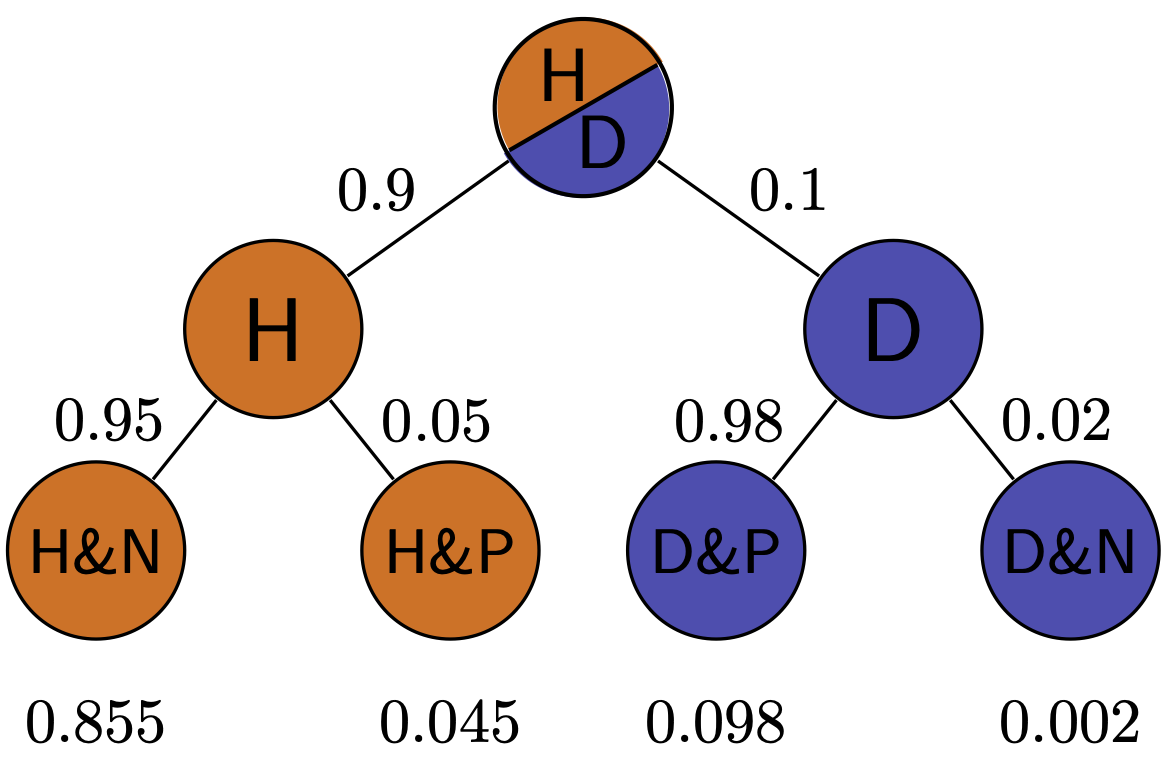
\includegraphics[width=0.5\linewidth,height=\textheight,keepaspectratio]{images/prob_tree_tikz1.png}

}

\caption{Bayesian hypothesis testing tree with prior probability 0.1}

\end{figure}%%
\begin{figure}[H]

{\centering 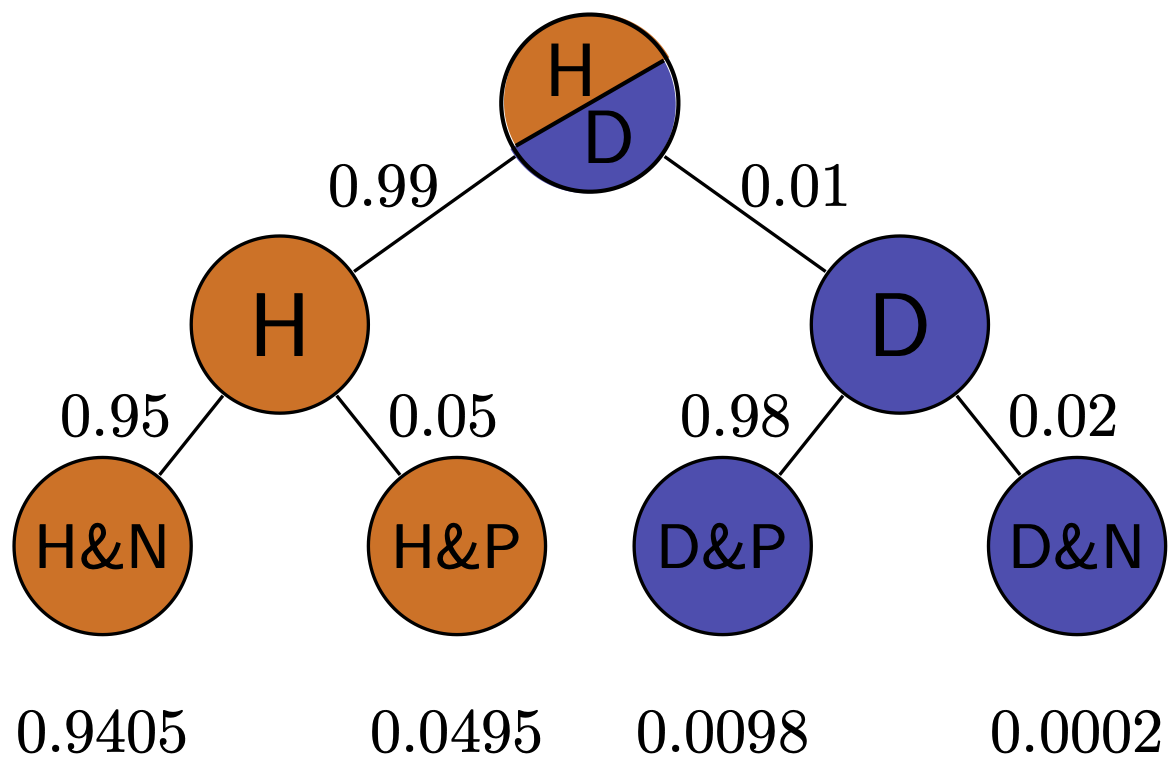
\includegraphics[width=0.5\linewidth,height=\textheight,keepaspectratio]{images/prob_tree_tikz2.png}

}

\caption{Bayesian hypothesis testing tree with prior probability 0.01}

\end{figure}%

\textbf{Exercise:} Simulate medical testing by rolling dice for a rare
disease (1/6 prevalence) and a common disease (1/2 prevalence), with
both sensitivity and specificity of 5/6. Compare the positive predictive
values for the two cases.

\subsection{prosecutor's fallacy}\label{prosecutors-fallacy}

\begin{Shaded}
\begin{Highlighting}[]
\NormalTok{\# Define variable containing URL}
\NormalTok{url \textless{}{-} "https://imgs.xkcd.com/comics/frequentists\_vs\_bayesians.png"}
\end{Highlighting}
\end{Shaded}

The basic principle of Bayesian thinking is that one cannot interpret
the reliability of a result, e.g.~a hypothesis test, without factoring
in the prior probability of it being true. This seems like a
commonsensical concept, but it is often neglected when such results are
interpreted in various contexts, which can lead to perilous mistakes.

Here is a scenario called ``the prosecutor's fallacy''. Suppose that a
defendant is accused of a crime, and physical evidence collected at the
crime scene matches this person (e.g.~a fingerprint or a DNA sample),
but no other evidence exists to connect the defendant to the crime. The
prosecutor calls an expert witness to testify that fewer than one out of
a million randomly chosen people would match this sample. Therefore, she
argues, there is overwhelming probability that the defendant is guilty
and less than 1 in a million chance they are innocent.

Do you spot the problem with the argument?

It's the same fallacy as we saw in the medical testing scenario, or that
is portrayed in the xkcd cartoon above. The prosecutor is conflating the
probability of a match (positive result) given that the person is
innocent, and the probability of the person being innocent, given the
match. The probability of the former is one in a million, but we want to
know the latter! And the latter depends on the prior probability of the
person committing the crime, which should have been investigated by the
detectives: did the defendant have a conflict with the victim or have
they never met? did he have opportunity to commit the crime, or was he
in a different city at the time? Without this information, it is
impossible to decide whether it's more likely that the DNA/fingerprint
match is a false positive (in a country of 300 million, you can find 300
false matches if everyone is in the database!) or a true positive.

\subsection{reproducibility in
science}\label{reproducibility-in-science}

In 2005 John Ioannidis published a paper entitled
\href{https://journals.plos.org/plosmedicine/article?id=10.1371/journal.pmed.0020124}{``Why
most published research findings are false''}. The paper, as you can see
by its title, was intended to be provocative, but it is based solidly on
the classic formula of Bayes. The motivation for the paper came from the
observation that too often in modern science, big, splashy studies that
were published could not be reproduced or verified by other researchers.
What could be behind this epidemic of questionable scientific work?

The problem as described by Ioannidis and many others, in a nutshell, is
that unthinking use of traditional hypothesis testing leads to a high
probability of false positive results being published. The paper
outlines several ways in which this can occur.

Too often, a hypothesis is tested and if the resultant p-value is less
than some arbitrary threshold (very often 0.05, an absurdly high
number), then the results are published. However, if one is testing a
hypothesis with low prior probability, a positive hypothesis test result
is very likely a false positive. Very often, modern biomedical research
involves digging through a large amount of information, like an entire
human genome, in search for associations between different genes and a
phenotype, like a disease. It is a priori unlikely that any specific
gene is linked to a given phenotype, because most genes have very
specific functions, and are expressed quite selectively, only at
specific times or in specific types of cells. However, publishing such
studies results in splashy headlines (``Scientists find a gene linked to
autism!'') and so a lot of false positive results are reported, only to
be refuted later, in much less publicized studies.

Ioannidis performed basic calculations of the probability that a
published study is true (that is, that a positive reported result is a
true positive), and how it is affected by pre-study (prior) probability,
number of conducted studies on the same hypothesis, and the level of
bias. His prediction is that for fairly typical scenario (e.g.~pre-study
probability of 10\%, ten groups working simultaneously, and a reasonable
amount of bias) the probability that a published result is correct is
less than 50\%. He then followed up with another paper {[}2{]} that
investigated 49 top-cited medical research publications over a decade,
and looked at whether follow-up studies could replicate the results, and
found that a very significant fraction of their findings could not be
replicated or were found to have weaker effects by subsequent
investigations.

\section{Bayesian inference}\label{bayesian-inference}

As an alternative to frequentist and maximum likelihood approaches to
modeling biological data, Bayesian statistics has seen an impressive
growth in recent years, due to the improved computational power.

At the heart of Bayesian inference is an application of Bayes' theorem:
take a model with parameters \(\theta\), and some data \(D\). Bayes'
theorem gives us a disciplined way to ``update'' our belief in the
distribution of \(\theta\) once we've seen the data \(D\):

\[
P(\theta \ \vert \ D) = \frac{P(D \ \vert \ \theta) P(\theta)}{P(D)}
\] where:

\begin{itemize}
\tightlist
\item
  \(P(\theta \ \vert \ D)\) is the \textbf{posterior distribution} of
  \(\theta\), i.e., our updated belief in the values of \(\theta\).
\item
  \(P(D \ \vert \ \theta)\) is the \textbf{likelihood function}:
  \(P(DX \ \vert \ \theta) = L(\theta \ \vert \ D)\).
\item
  \(P(\theta)\) is the \textbf{prior distribution}, i.e.~our belief on
  the distribution of \(\theta\) before seeing the data.
\item
  \(P(D)\) is called the \textbf{evidence}:
  \(P(D) = \int P(D \ \vert \ \theta) d \theta\) (in practice, this need
  not to be calculated).
\end{itemize}

\subsection{Example: capture-recapture}\label{example-capture-recapture}

There is a well-established method in population ecology of estimating
the size of a population by repeatedly capturing and tagging a number of
individuals and later repeating the experiment to see how many are
recaptured. Suppose that \(n\) were captured initially and \(k\) were
recaptured later. We assume that the probability \(p\) of recapturing an
individual is the same for all individuals. Then our likelihood function
is once again, based on the binomial distribution.

\[
L(p \ \vert \ k, n) = \binom{n}{k}p^k (1-p)^{n-k}
\] and our maximum likelihood estimate is \(\hat{p} = k /n\). This
allows for estimation of the total population size to be
\(P = n_2/\hat p\), where \(n_2\) is the total number of individuals
captured in the second experiment. There are more sophisticated
estimators, but this one is reasonable for large enough populations.

Let us plot the likelihood as a function of \(p\) for the case in which
\(n = 100\) and \(k = 33\)

\begin{Shaded}
\begin{Highlighting}[]
\NormalTok{n \textless{}{-} 100}
\NormalTok{m \textless{}{-} 33}
\NormalTok{pl \textless{}{-} ggplot(data = data.frame(x = 0, y = 0)) + xlim(c(0,1))}
\NormalTok{likelihood\_function \textless{}{-} function(p) \{}
\NormalTok{  lik \textless{}{-} choose(n, m) * p\^{}m * (1{-}p)\^{}(n {-} m)}
\NormalTok{  \# divide by the evidence to make into density function}
\NormalTok{  return(lik * (n + 1))}
\NormalTok{\}}
\NormalTok{pl \textless{}{-} pl + stat\_function(fun = likelihood\_function)}
\NormalTok{show(pl)}
\end{Highlighting}
\end{Shaded}

Now we choose a prior. For convenience, we choose a Beta distribution,
\(P(p) = \text{Beta}(\alpha, \beta) = \frac{p^{\alpha - 1} (1-p)^{\beta - 1}}{B(\alpha, \beta)}\),
where \(B(\alpha, \beta)\) is the Beta function,
\(B(\alpha, \beta) = \int_0^1 t^{\alpha -1} (1-t)^{\beta - 1} dt\).

Therefore:

\[
\begin{aligned}
P(p \ \ \vert \ \ m,n) & \propto L(p \ \ \vert \ \ m,n) P(p) \\
&= \left(\binom{n}{m} p^m (1-p)^{n-m} \right) \left( \frac{p^{\alpha - 1} (1-p)^{\beta - 1}}{B(\alpha, \beta)} \right)\\
& \propto p^{m+\alpha -1} (1-p)^{n-m + \beta -1} \\
& \propto \text{Beta}(m + \alpha, \beta + m - n)
\end{aligned}
\]

We can explore the effect of choosing a prior on the posterior. Suppose
that in the past we have seen probabilities close to 50\%. Then we could
choose a prior \(\text{Beta}(10,10)\) (this is what is called a
``strong'' or ``informative'' prior). Let's see what happens to the
posterior:

\begin{Shaded}
\begin{Highlighting}[]
\NormalTok{\# a strong prior}
\NormalTok{alpha \textless{}{-} 10}
\NormalTok{beta \textless{}{-} 10}
\NormalTok{prior\_function \textless{}{-} function(p) dbeta(p, alpha, beta)}
\NormalTok{posterior\_function \textless{}{-} function(p) dbeta(p, alpha + m, beta + n {-} m)}
\NormalTok{pl + stat\_function(fun = prior\_function, colour = "blue") + }
\NormalTok{  stat\_function(fun = posterior\_function, colour = "red")}
\end{Highlighting}
\end{Shaded}

You can see that the posterior ``mediates'' between the prior and the
likelihood curve. When we use a weak prior, then our posterior will be
closer to the likelihood function:

\begin{Shaded}
\begin{Highlighting}[]
\NormalTok{\# a weak prior}
\NormalTok{alpha \textless{}{-} 1/2}
\NormalTok{beta \textless{}{-} 1/2}
\NormalTok{pl + stat\_function(fun = prior\_function, colour = "blue") + }
\NormalTok{  stat\_function(fun = posterior\_function, colour = "red")}
\end{Highlighting}
\end{Shaded}

The fact that the posterior depends on the prior is the most
controversial aspect of Bayesian inference. Different schools of thought
treat this feature differently (e.g., ``Subjective Bayes'' interprets
priors as beliefs before seeing the data; ``Empirical Bayes'' relies on
previous experiments or on the data themselves to derive the prior;
``Objective Bayes'' tries to derive the least-informative prior given
the data). In practice, the larger the data, the cleaner the signal, the
lesser the influence of the prior on the resulting posterior.

\subsection{MCMC}\label{mcmc}

The type of calculation performed above is feasible only for very simple
models, and for appropriately chosen priors (called ``conjugate
priors''). For more complex models, we rely on simulations. In
particular, one can use Markov-Chain Monte Carlo (MCMC) to sample from
the posterior distribution of complex models. Very briefly, one builds a
Markov-Chain in which the states represent sets of parameters;
parameters are sampled from the prior, and the probability of moving to
one state to another is proportional to the difference in their
likelihood. When the MC converges, then one obtains the posterior
distribution of the parameters.

Bayesian inference is used for many complex problems, including
phylogenetic tree building {[}5{]}.

\section{Reading:}\label{reading}

\begin{enumerate}
\def\labelenumi{\arabic{enumi}.}
\item
  \href{https://www.r-bloggers.com/maximum-likelihood-estimation-from-scratch/}{Maximum
  likelihood estimation from scratch}
\item
  \href{https://academic.oup.com/mbe/article/24/8/1586/1103731}{Phylogenetic
  Analysis by Maximum Likelihood}
\item
  \href{https://journals.plos.org/plosmedicine/article?id=10.1371/journal.pmed.0020124}{Why
  most published scientific studies are false}
\item
  \href{https://jamanetwork.com/journals/jama/fullarticle/201218}{Contradicted
  and Initially Stronger Effects in Highly Cited Clinical Research}
\item
  \href{http://nbisweden.github.io/MrBayes/}{MrBayes}
\item
  \href{https://www.molecularecologist.com/2016/02/quick-and-dirty-tree-building-in-r/}{Quick
  and Dirty Tree Building in R}
\item
  \href{https://en.wikipedia.org/wiki/Mark_and_recapture}{Mark and
  Recapture}
\end{enumerate}

\bookmarksetup{startatroot}

\chapter{Review of linear algebra}\label{review-of-linear-algebra}

\textbf{Goals}

\begin{itemize}
\tightlist
\item
  Solving linear equations
\item
  Best-fit line through multiple data points
\item
  Concepts of linearity and vector spaces
\item
  Representation of vectors in multiple bases
\item
  Eigenvalues and eigenvectors of matrices
\end{itemize}

\section{Solving multivariate linear
equations}\label{solving-multivariate-linear-equations}

Linear algebra is intimately tied to linear equations, that is, to
equations where all variables are multiplied by constant terms and added
together. Linear equations with one variable are easily solved by
division, for example:

\[
4x = 20
\]

is solved by dividing both sides by 4, obtaining the unique solution
\(x=5\).

The situation gets more interesting when multiple variables are
involved, with multiple equations, for example:

\[
\begin{aligned}
4x - 3y &= 5 \\
 -x + 2y &= 10
\end{aligned}
\]

There are multiple ways to solve this, for example solving one equation
for one variable in terms of the other, then substituting it into the
second equation to obtain a one-variable problem. A more general
approach involves writing this problem in terms of a matrix
\(\mathbf A\) that contains the multiplicative constants of \(x\) and
\(y\) and a vector \(\vec b\) that contains the right-hand side
constants:

\[
\begin{aligned}
\mathbf{A} = \begin{pmatrix} 4 & -3 \\ -1 & 2 \end{pmatrix} \;\;\; \vec{b} = \begin{pmatrix}5 \\ 10 \end{pmatrix} &\;\;\;
\vec{x} = \begin{pmatrix} x \\ y \end{pmatrix} \\
\mathbf{A} \vec x = \vec b &
\end{aligned}
\]

This now looks analogous to the one-variable equation above, which we
solved by dividing both sides by the multiple of \(x\). The difficulty
is that matrix operations are more complicated than scalar
multiplication and division. Matrix multiplication is used in the
equation above to multiply all the coefficients in the matrix by their
respective variables, which involves a relatively complicated
\href{https://en.wikipedia.org/wiki/Matrix_multiplication}{procedure in
general}.

The ``division'' equivalent is called
\href{https://en.wikipedia.org/wiki/Invertible_matrix}{matrix inversion}
and it is even more complicated. First, we need to define the identity
matrix, or the equivalent of the number 1 for matrix multiplication. The
identity matrix is defined only for square matrices (equal number of
rows and columns), so a size \(n\) by \(n\) identity matrix is define to
have all 1s on the diagonal and all zeros on the off-diagonal: \[
I = \begin{pmatrix} 1 & 0 & \dots & 0 \\ 0 & 1  &\dots & 0 \\ \vdots & \vdots & \ddots & \vdots \\ 0 & 0 &\dots & 1\end{pmatrix}
\] The identity matrix is special because multiplying any other matrix
(of compatible size) by it results in the same exact matrix (this is
easy to check on a couple of examples for \(2 \times 2\) or
\(3 \times 3\) matrices):

\[
I A = A I = A
\] Then for an \(n\) by \(n\) matrix \(A\) its inverse \(A^{-1}\) is
defined to be the matrix multiplication by which results in the identity
matrix, that is: \[
A^{-1} A = A A^{-1}  = I
\] Defining the inverse is one task, but calculating it for any given
matrix, especially of large size, is quite laborious. We will not
describe the algorithms here, but you can read about
\href{https://en.wikipedia.org/wiki/Gaussian_elimination\#Finding_the_inverse_of_a_matrix}{Gauss-Jordan
elimination}, which is one classic example. One important point is that
not all matrices are invertible, and for some no inverse matrix exists,
analogous to zero for real number division. The difference is that there
are infinitely many matrices for which this is the case, called
\emph{singular} matrices.

In the cases in which the inverse matrix exists, the linear system of
equations can be solved by multiplying both sides by the inverse matrix,
like this: \[
 \vec x = \mathbf{A}^{-1}\vec b
\]

\emph{Example:} Take the linear \(2 \times 2\) system of equations of
above and solve it using matrix inversion.The \texttt{R} function
\texttt{solve()} calculates the inverse and multiplies it by the
constant vector \texttt{b}:

\begin{Shaded}
\begin{Highlighting}[]
\NormalTok{A \textless{}{-} matrix(c(4,{-}1,{-}3,2), nrow = 2)}
\NormalTok{b \textless{}{-} c(5,10)}
\NormalTok{solve(A,b)}
\end{Highlighting}
\end{Shaded}

\section{Fitting a line to data}\label{fitting-a-line-to-data}

One geometric application of solving multiple linear equations is to
find the coefficients of a line that passes through two points in the
2-dimensional plane (or of a plane that passes through three points in
three-dimensional space, but we won't go there.) In that case, the
coordinates of the points are the data, and the unknown variables are
the parameters slope \(m\) and intercept \(b\) of the line that we want
to find.

\textbf{Example:} If the data set consists of two points
\((3,5), (6, 2)\), then finding the best fit values of \(m\) and \(b\)
means solving the following two equations:

\[
\begin{aligned}
 3m + b &= 5 \\
 6m + b &= 2
\end{aligned}
\]

These equations have a solution for the slope and intercept, which can
be calculated in \texttt{R} using \texttt{solve()} and then plot the
line with the parameters from the solution vector \texttt{beta}:

\begin{Shaded}
\begin{Highlighting}[]
\NormalTok{xs \textless{}{-} c(3, 6)}
\NormalTok{ys \textless{}{-} c(5, 2)}
\NormalTok{A \textless{}{-} matrix(c(xs[1], xs[2], 1, 1), nrow = 2)}
\NormalTok{b \textless{}{-} c(ys[1], ys[2])}
\NormalTok{beta \textless{}{-} solve(A, b)}
\NormalTok{data1 \textless{}{-} tibble(xs, ys)}
\NormalTok{ggplot(data = data1) + }
\NormalTok{  aes(x = xs, y = ys) + }
\NormalTok{  geom\_point() + }
\NormalTok{  geom\_abline(slope = beta[1], intercept = beta[2])}
\end{Highlighting}
\end{Shaded}

However, a data set with two points is very small and nobody would
accept these values as reasonable estimates. Let us add one more data
point, to increase our sample size to three: \((3,5), (6, 2), (9, 1)\).
How do you find the best fit slope and intercept?

\textbf{Bad idea:} take two points and find a line, that is the slope
and the intercept, that passes through the two. It should be clear why
this is a bad idea: we are arbitrarily ignoring some of the data, while
perfectly fitting two points. So how do we use all the data? Let us
write down the equations that a line with slope \(m\) and intercept
\(b\) have to satisfy in order to fit our data points:

\[
\begin{aligned}
3m + b = 5 \\
6m + b = 2\\
9m + b = 1
\end{aligned}
\]

This system has no exact solution, since there are three equations and
only two unknowns. We need to find \(m\) and \(b\) such that they are a
``best fit'' to the data, not the perfect solution.

\subsection{Least-squares line}\label{least-squares-line}

Let us write the equation in matrix form as follows:

\[
\begin{aligned}
\mathbf{A} = \begin{pmatrix} 3 & 1 \\ 6 & 1 \\ 9 & 1 \end{pmatrix} \;\;\; \vec{b} = \begin{pmatrix}5 \\ 2 \\ 1 \end{pmatrix} \;\;\;
\vec{\beta} = \begin{pmatrix} m \\ b \end{pmatrix} \\
\mathbf{A} \vec \beta = \vec b 
\end{aligned}
\]

Mathematically, the problem is that one cannot invert a non-square
matrix. However, there is a way of turning the matrix into a square one,
by multiplying it by its own transpose (same matrix with rows and
columns reversed):

\[
\mathbf{A}^T \mathbf{A} \vec \beta = \mathbf{A}^T \vec b
\] \emph{Exercise:} Carry out the matrix multiplications to verify that
\(\mathbf{A}^T \mathbf{A}\) is a \(2 \times 2\) matrix and
\(\mathbf{A}^T \vec b\) is a vector of length 2.

Now we can solve this equation with a square matrix
\(\mathbf{A}^T \mathbf{A}\) by multiplying both sides by the inverse! In
general, for an \(n\)-dimensional data set consisting of a bunch of
values of \(x\) and \(y\), the process looks like this:

\[
\vec Y = \begin{pmatrix} y_1\\ y_2\\ \vdots \\ y_n \end{pmatrix} \;\;\; 
\mathbf{X} = \begin{pmatrix} 1 & x_1\\ 1 & x_2\\ \vdots & \vdots \\ 1 & x_n \end{pmatrix}
 \;\;\; 
\mathbf{\beta} = \begin{pmatrix} m \\ b \end{pmatrix} \\
\beta = (\mathbf{X}^{T} \mathbf{X})^{-1} \mathbf{X}^{T}\vec Y
\] \emph{Example:} Let us see the best-fit line for the 3-point data set
above:

\begin{Shaded}
\begin{Highlighting}[]
\NormalTok{xs \textless{}{-} c(3, 6, 9)}
\NormalTok{ys \textless{}{-} c(5, 2, 1)}
\NormalTok{A \textless{}{-} matrix(c(xs[1], xs[2], xs[3], 1, 1, 1), nrow = 3)}
\NormalTok{b \textless{}{-} c(ys[1], ys[2], ys[3])}
\NormalTok{beta \textless{}{-} solve(t(A) \%*\% A, t(A) \%*\% b)}
\NormalTok{data1 \textless{}{-} tibble(xs, ys)}
\NormalTok{ggplot(data = data1) + }
\NormalTok{  aes(x = xs, y = ys) + }
\NormalTok{  geom\_point() + }
\NormalTok{  geom\_abline(slope = beta[1], intercept = beta[2])}
\end{Highlighting}
\end{Shaded}

Let us use the classic data set of Karl Pearson's from 1903 containing
the height of fathers and sons, which we will return to next week when
we tackle linear regression properly:

\begin{Shaded}
\begin{Highlighting}[]
\NormalTok{library(UsingR)}
\NormalTok{data("father.son")}
\NormalTok{pl \textless{}{-} ggplot(data = father.son) + }
\NormalTok{  aes(x = fheight, y = sheight) + }
\NormalTok{  geom\_point() + }
\NormalTok{  coord\_equal()}
\NormalTok{pl}
\end{Highlighting}
\end{Shaded}

\emph{Exercise:} Let's try to find the best fit line to this data set
(the hard way) using the same process as above for the three - point
data set:

\begin{Shaded}
\begin{Highlighting}[]

\end{Highlighting}
\end{Shaded}

Of course, \texttt{R} can do this calculation for you with just one
command:

\begin{Shaded}
\begin{Highlighting}[]
\NormalTok{best\_beta\_easy \textless{}{-} lm(sheight \textasciitilde{} fheight, data = father.son)}
\NormalTok{best\_beta\_easy}
\end{Highlighting}
\end{Shaded}

But it feels good to know that this is not black magic! In fact,
plotting it on top of the data does not even require computing the
coefficients:

\begin{Shaded}
\begin{Highlighting}[]
\NormalTok{pl + geom\_smooth(method = "lm") \# lm stands for linear model}
\end{Highlighting}
\end{Shaded}

\section{Linearity and vector spaces}\label{linearity-and-vector-spaces}

We have dealt with linear models in various guises, so now would be a
good time to define properly what linearity means. The word comes from
the shape of graphs of linear functions of one variable,
e.g.~\(f(x) = a x + b\), but the algebraic meaning rests on the
following two general properties:

\textbf{Definition.} A \emph{linear transformation} or \emph{linear
operator} is a mapping \(L\) between two sets of vectors with the
following properties:

\begin{enumerate}
\def\labelenumi{\arabic{enumi}.}
\tightlist
\item
  \emph{(scalar multiplication)} \(L(c \vec v) = c L(\vec v)\); where
  \(c\) is a scalar and \(\vec v\) is a vector
\item
  \emph{(additive)}
  \(L(\vec v_1 + \vec v_2) = L(\vec v_1) + L(\vec v_2)\); where
  \(\vec v_1\) and \(\vec v_2\) are vectors
\end{enumerate}

Here we have two types of objects: vectors and transformations/operators
that act on those vectors. The basic example of this are vectors and
matrices, because a matrix multiplied by a column vector (on the right)
results in another column vector, provided the number of columns in the
matrix is the same as the number of rows in the vector. This can be
interpreted as the matrix transforming the vector \(\vec v\) into
another one: \(A \times \vec v = \vec u\).

\textbf{Example:} Let us multiply the following matrix and vector
(specially chosen to make a point):

\begin{Shaded}
\begin{Highlighting}[]
\NormalTok{A \textless{}{-} matrix(c(2, 2, 1, 3), nrow = 2)}
\NormalTok{vec1 \textless{}{-} c(1, {-}1)}
\NormalTok{vec2 \textless{}{-} A \%*\% vec1}
\NormalTok{print(vec1)}
\NormalTok{print(vec2)}
\end{Highlighting}
\end{Shaded}

We see that this particular vector \((1,-1)\) is unchanged when
multiplied by this matrix, or we can say that the matrix multiplication
is equivalent to multiplication by 1. Here is another such vector for
the same matrix:

\begin{Shaded}
\begin{Highlighting}[]
\NormalTok{vec1 \textless{}{-} c(1, 2)}
\NormalTok{vec2 \textless{}{-} A \%*\% vec1}
\NormalTok{print(vec1)}
\NormalTok{print(vec2)}
\end{Highlighting}
\end{Shaded}

In this case, the vector is changed, but only by multiplication by a
constant (4). Thus the geometric direction of the vector remained
unchanged.

The notion of linearity leads to the important idea of combining
different vectors:

\textbf{Definition:} A \emph{linear combination} of \(n\) vectors
\(\{ \vec v_i \}\) is a weighted sum of these vectors with any real
numbers \(\{a_i\}\): \[ a_1 \vec v_1+ a_2 \vec v_2... + a_n \vec v_n\]

Linear combinations arise naturally from the notion of linearity,
combining the additive property and the scalar multiplication property.
Speaking intuitively, a linear combination of vectors produces a new
vector that is related to the original set. Linear combinations give a
simple way of generating new vectors, and thus invite the following
definition for a collection of vectors closed under linear combinations:

\textbf{Definition.} A \emph{vector space} is a collection of vectors
such that a linear combination of any \(n\) vectors is contained in the
vector space.

The most common examples are the spaces of all real-valued vectors of
dimension \(n\), which are denoted by \(\mathbb{webr-r}^n\). For
instance, \(\mathbb{webr-r}^2\) (pronounced ``r two'') is the vector
space of two dimensional real-valued vectors such as \((1,3)\) and
\((\pi, -\sqrt{17})\); similarly, \(\mathbb{webr-r}^3\) is the vector
space consisting of three dimensional real-valued vectors such as
\((0.1,0,-5.6)\). You can convince yourself, by taking linear
combinations of vectors, that these vector spaces contain all the points
in the usual Euclidean plane and three-dimensional space. The real
number line can also be thought of as the vector space
\(\mathbb{webr-r}^1\).

\subsection{Linear independence and basis
vectors}\label{linear-independence-and-basis-vectors}

How can we describe a vector space without trying to list all of its
elements? We know that one can generate an element by taking linear
combinations of vectors. It turns out that it is possible to generate
(or ``span'') a vector space by taking linear combinations of a subset
of its vectors. The challenge is to find a minimal subset of subset that
is not redundant. In order to do this, we first introduce a new concept:

\textbf{Definition:} A set of vectors \(\{ \vec v_i \}\) is called
\emph{linearly independent} if the only linear combination involving
them that equals the zero vector is if all the coefficients are zero. (
\(a_1 \vec v_1 + a_2 \vec v_2 + ... + a_n \vec v_n = 0\) only if
\(a_i = 0\) for all \(i\).)

In the familiar Euclidean spaces, e.g.~\(\mathbb{webr-r}^2\), linear
independence has a geometric meaning: two vectors are linearly
independent if the segments from the origin to the endpoint do not lie
on the same line. But it can be shown that any set of three vectors in
the plane is linearly dependent, because there are only two dimensions
in the vector space. This brings us to the key definition of this
section:

\textbf{Definition:} A \emph{basis} of a vector space is a linearly
independent set of vectors that generate (or span) the vector space. The
number of vectors (cardinality) in such a set is called the
\emph{dimension} of the vector space.

A vector space generally has many possible bases, as illustrated in
figure. In the case of \(\mathbb{webr-r}^2\), the usual (canonical)
basis set is \(\{(1,0); (0,1)\}\) which obviously generates any point on
the plane and is linearly independent. But any two linearly independent
vectors can generate any vector in the plane.

\textbf{Example:} The vector \(\vec r = (2,1)\) can be represented as a
linear combination of the two canonical vectors:
\(\vec r = 2\times (1,0)+1\times (0,1)\). Let us choose another basis
set, say \(\{(1,1); (-1,1)\}\) (this is the canonical basis vectors
rotated by \(\pi/2\).) The same vector can be represented by a linear
combination of these two vectors, with coefficients \(1.5\) and
\(-0.5\): \(\vec r = 1.5\times (1,1) - 0.5 \times (-1,1)\). If we call
the first basis \(C\) for canonical and the second basis \(D\) for
different, we can write the same vector using different sets of
coordinates for each basis:

\[ 
\vec r_{C} = (2,1); \; \vec r_D = (1.5, -0.5)
\]

\subsection{Projections and changes of
basis}\label{projections-and-changes-of-basis}

The representation of an arbitrary vector (point) in a vector space as a
linear combination of a given basis set is called the
\emph{decomposition} of the point in terms of the basis, which gives the
coordinates for the vector in terms of each basis vector. The
decomposition of a point in terms of a particular basis is very useful
in high-dimensional spaces, where a clever choice of a basis can allow a
description of a set of points (such as a data set) in terms of
contributions of only a few basis vectors, if the data set primarily
extends only in a few dimensions.

To obtain the coefficients of the basis vectors in a decomposition of a
vector \(\vec r\), we need to perform what is termed a \emph{projection}
of the vector onto the basis vectors. Think of shining a light
perpendicular to the basis vector, and measuring the length of the
shadow cast by the vector \(\vec r\) onto \(\vec v_i\). If the vectors
are parallel, the shadow is equal to the length of \(\vec r\); if they
are orthogonal, the shadow is nonexistent. To find the length of the
shadow, use the inner product of \(\vec r\) and \(\vec v\), which as you
recall corresponds to the cosine of the angle between the two vectors
multiplied by their norms:
\(\left\langle \vec r, \vec v\right \rangle =\vert\vec r\vert \vert\vec v\vert\cos(\theta)\).
We do not care about the length of the vector \(\vec v\) we are
projecting onto, thus we divide the inner product by the square norm of
\(\vec v\), and then multiply the vector \(\vec v\) by this projection
coefficient:

\[ 
Proj(\vec r ; \vec v) = \frac{ \langle \vec r , \vec v \rangle  } {\langle \vec v , \vec v \rangle } \vec v = \frac{ \langle \vec r ,  \vec v \rangle  } {\vert \vec v \vert^2} \vec v= \frac{  \vert\vec r\vert \cos(\theta) } {\vert \vec v \vert}\vec v
\]

This formula gives the projection of the vector \(\vec r\) onto
\(\vec v\), the result is a new vector in the direction of \(\vec v\),
with the scalar coefficient
\(a = \ \langle \vec r , \vec v \rangle /\vert \vec v \vert^2\).

\textbf{Example:} Here is how one might calculate the projection of the
point \((2,1)\) onto the basis set \(\{(1,1); (-1,1)\}\):

\begin{Shaded}
\begin{Highlighting}[]
\NormalTok{v1 \textless{}{-} c(1, 1)}
\NormalTok{v2 \textless{}{-} c({-}1, 1)}
\NormalTok{u \textless{}{-} c(2, 1)}
\NormalTok{ProjMat \textless{}{-} matrix(cbind(v1, v2), }
\NormalTok{                  byrow = T, nrow = 2)}
\NormalTok{print(ProjMat)}
\NormalTok{ProjMat \%*\% u}
\end{Highlighting}
\end{Shaded}

This is not quite right: the projection coefficients are off by a factor
of two compared to the correct values in the example above. This is
because we have neglected to \emph{normalize} the basis vectors, so we
should modify the script as follows:

\begin{Shaded}
\begin{Highlighting}[]
\NormalTok{v1 \textless{}{-} c(1, 1)}
\NormalTok{v1 \textless{}{-} v1 / (sum(v1\^{}2))}
\NormalTok{v2 \textless{}{-} c({-}1, 1)}
\NormalTok{v2 \textless{}{-} v2 / (sum(v2\^{}2))}
\NormalTok{u \textless{}{-} c(2, 1)}
\NormalTok{ProjMat \textless{}{-} matrix(cbind(v1, v2), }
\NormalTok{                  byrow = T, nrow = 2)}
\NormalTok{print(ProjMat)}
\NormalTok{print(ProjMat \%*\% u)}
\end{Highlighting}
\end{Shaded}

This is an example of how to convert a vector/point from representation
in one basis set to another. The new basis vectors, expressed in the
original basis set, are arranged in a matrix by row, scaled by their
norm squared, and multiplied by the vector that one wants to express in
the new basis. The resulting vector contains the coordinates in the new
basis.

\section{Matrices as linear
operators}\label{matrices-as-linear-operators}

\subsection{Matrices transform
vectors}\label{matrices-transform-vectors}

In this section we will learn to characterize square matrices by finding
special numbers and vectors associated with them. At the core of this
analysis lies the concept of a matrix as an \emph{operator} that
transforms vectors by multiplication. To be clear, in this section we
take as default that the matrices \(A\) are square, and that vectors
\(\vec v\) are column vectors, and thus will multiply the matrix on the
right: \(A \times \vec v\).

A matrix multiplied by a vector produces another vector, provided the
number of columns in the matrix is the same as the number of rows in the
vector. This can be interpreted as the matrix transforming the vector
\(\vec v\) into another one: \(A \times \vec v = \vec u\). The resultant
vector \(\vec u\) may or may not resemble \(\vec v\), but there are
special vectors for which the transformation is very simple.

\textbf{Example.} Let us multiply the following matrix and vector
(specially chosen to make a point):

\[
\left(\begin{array}{cc}2 & 1 \\ 2& 3\end{array}\right)\left(\begin{array}{c}1 \\ -1 \end{array}\right) = \left(\begin{array}{c}2 -1 \\ 2 - 3 \end{array}\right) =  \left(\begin{array}{c} 1 \\ -1 \end{array}\right)
\]

We see that this particular vector is unchanged when multiplied by this
matrix, or we can say that the matrix multiplication is equivalent to
multiplication by 1. Here is another such vector for the same matrix:

\[
\left(\begin{array}{cc}2 & 1 \\ 2& 3\end{array}\right)\left(\begin{array}{c}1 \\ 2 \end{array}\right) = \left(\begin{array}{c}2 +2 \\ 2 + 6 \end{array}\right) =  \left(\begin{array}{c} 4 \\ 8 \end{array}\right)
\]

In this case, the vector is changed, but only by multiplication by a
constant (4). Thus the geometric direction of the vector remained
unchanged.

Generally, a square matrix has an associated set of vectors for which
multiplication by the matrix is equivalent to multiplication by a
constant. This can be written down as a definition:

\textbf{Definition.} An \emph{eigenvector} of a square matrix \(A\) is a
vector \(\vec v\) for which matrix multiplication by \(A\) is equivalent
to multiplication by a constant. This constant \(\lambda\) is called its
\emph{eigenvalue} of \(A\) corresponding the the eigenvector \(\vec v\).
The relationship is summarized in the following equation:

\[
A  \times  \vec v = \lambda \vec v
\]

Note that this equation combines a matrix (\(A\)), a vector (\(\vec v\))
and a scalar \(\lambda\), and that both sides of the equation are column
vectors.

The definition does not specify how many such eigenvectors and
eigenvalues can exist for a given matrix \(A\). There are usually as
many such vectors \(\vec v\) and corresponding numbers \(\lambda\) as
the number of rows or columns of the square matrix \(A\), so a 2 by 2
matrix has two eigenvectors and two eigenvalues, a 5x5 matrix has 5 of
each, etc. One ironclad rule is that there cannot be more distinct
eigenvalues than the matrix dimension. Some matrices possess fewer
eigenvalues than the matrix dimension, those are said to have a
\emph{degenerate} set of eigenvalues, and at least two of the
eigenvectors share the same eigenvalue.

The situation with eigenvectors is trickier. There are some matrices for
which any vector is an eigenvector, and others which have a limited set
of eigenvectors. What is difficult about counting eigenvectors is that
an eigenvector is still an eigenvector when multiplied by a constant.
You can show that for any matrix, multiplication by a constant is
commutative: \(cA = Ac\), where \(A\) is a matrix and \(c\) is a
constant. This leads us to the important result that if \(\vec v\) is an
eigenvector with eigenvalue \(\lambda\), then any scalar multiple
\(c \vec v\) is also an eigenvector with the same eigenvalue. The
following demonstrates this algebraically:

\[
A  \times  (c \vec v) = c A  \times  \vec v = c \lambda \vec v =  \lambda (c \vec v)
\]

This shows that when the vector \(c \vec v\) is multiplied by the matrix
\(A\), it results in its being multiplied by the same number
\(\lambda\), so by definition it is an eigenvector. Therefore, an
eigenvector \(\vec v\) is not unique, as any constant multiple
\(c \vec v\) is also an eigenvector. It is more useful to think not of a
single eigenvector \(\vec v\), but of a \textbf{collection of vectors
that can be inter-converted by scalar multiplication} that are all
essentially the same eigenvector. Another way to represent this, if the
eigenvector is real, is that an eigenvector as a \textbf{direction that
remains unchanged by multiplication by the matrix}, such as direction of
the vector \(v\) in the figure below. As mentioned above, this is true
only for real eigenvalues and eigenvectors, since complex eigenvectors
cannot be used to define a direction in a real space.

\begin{figure}[H]

{\centering \pandocbounded{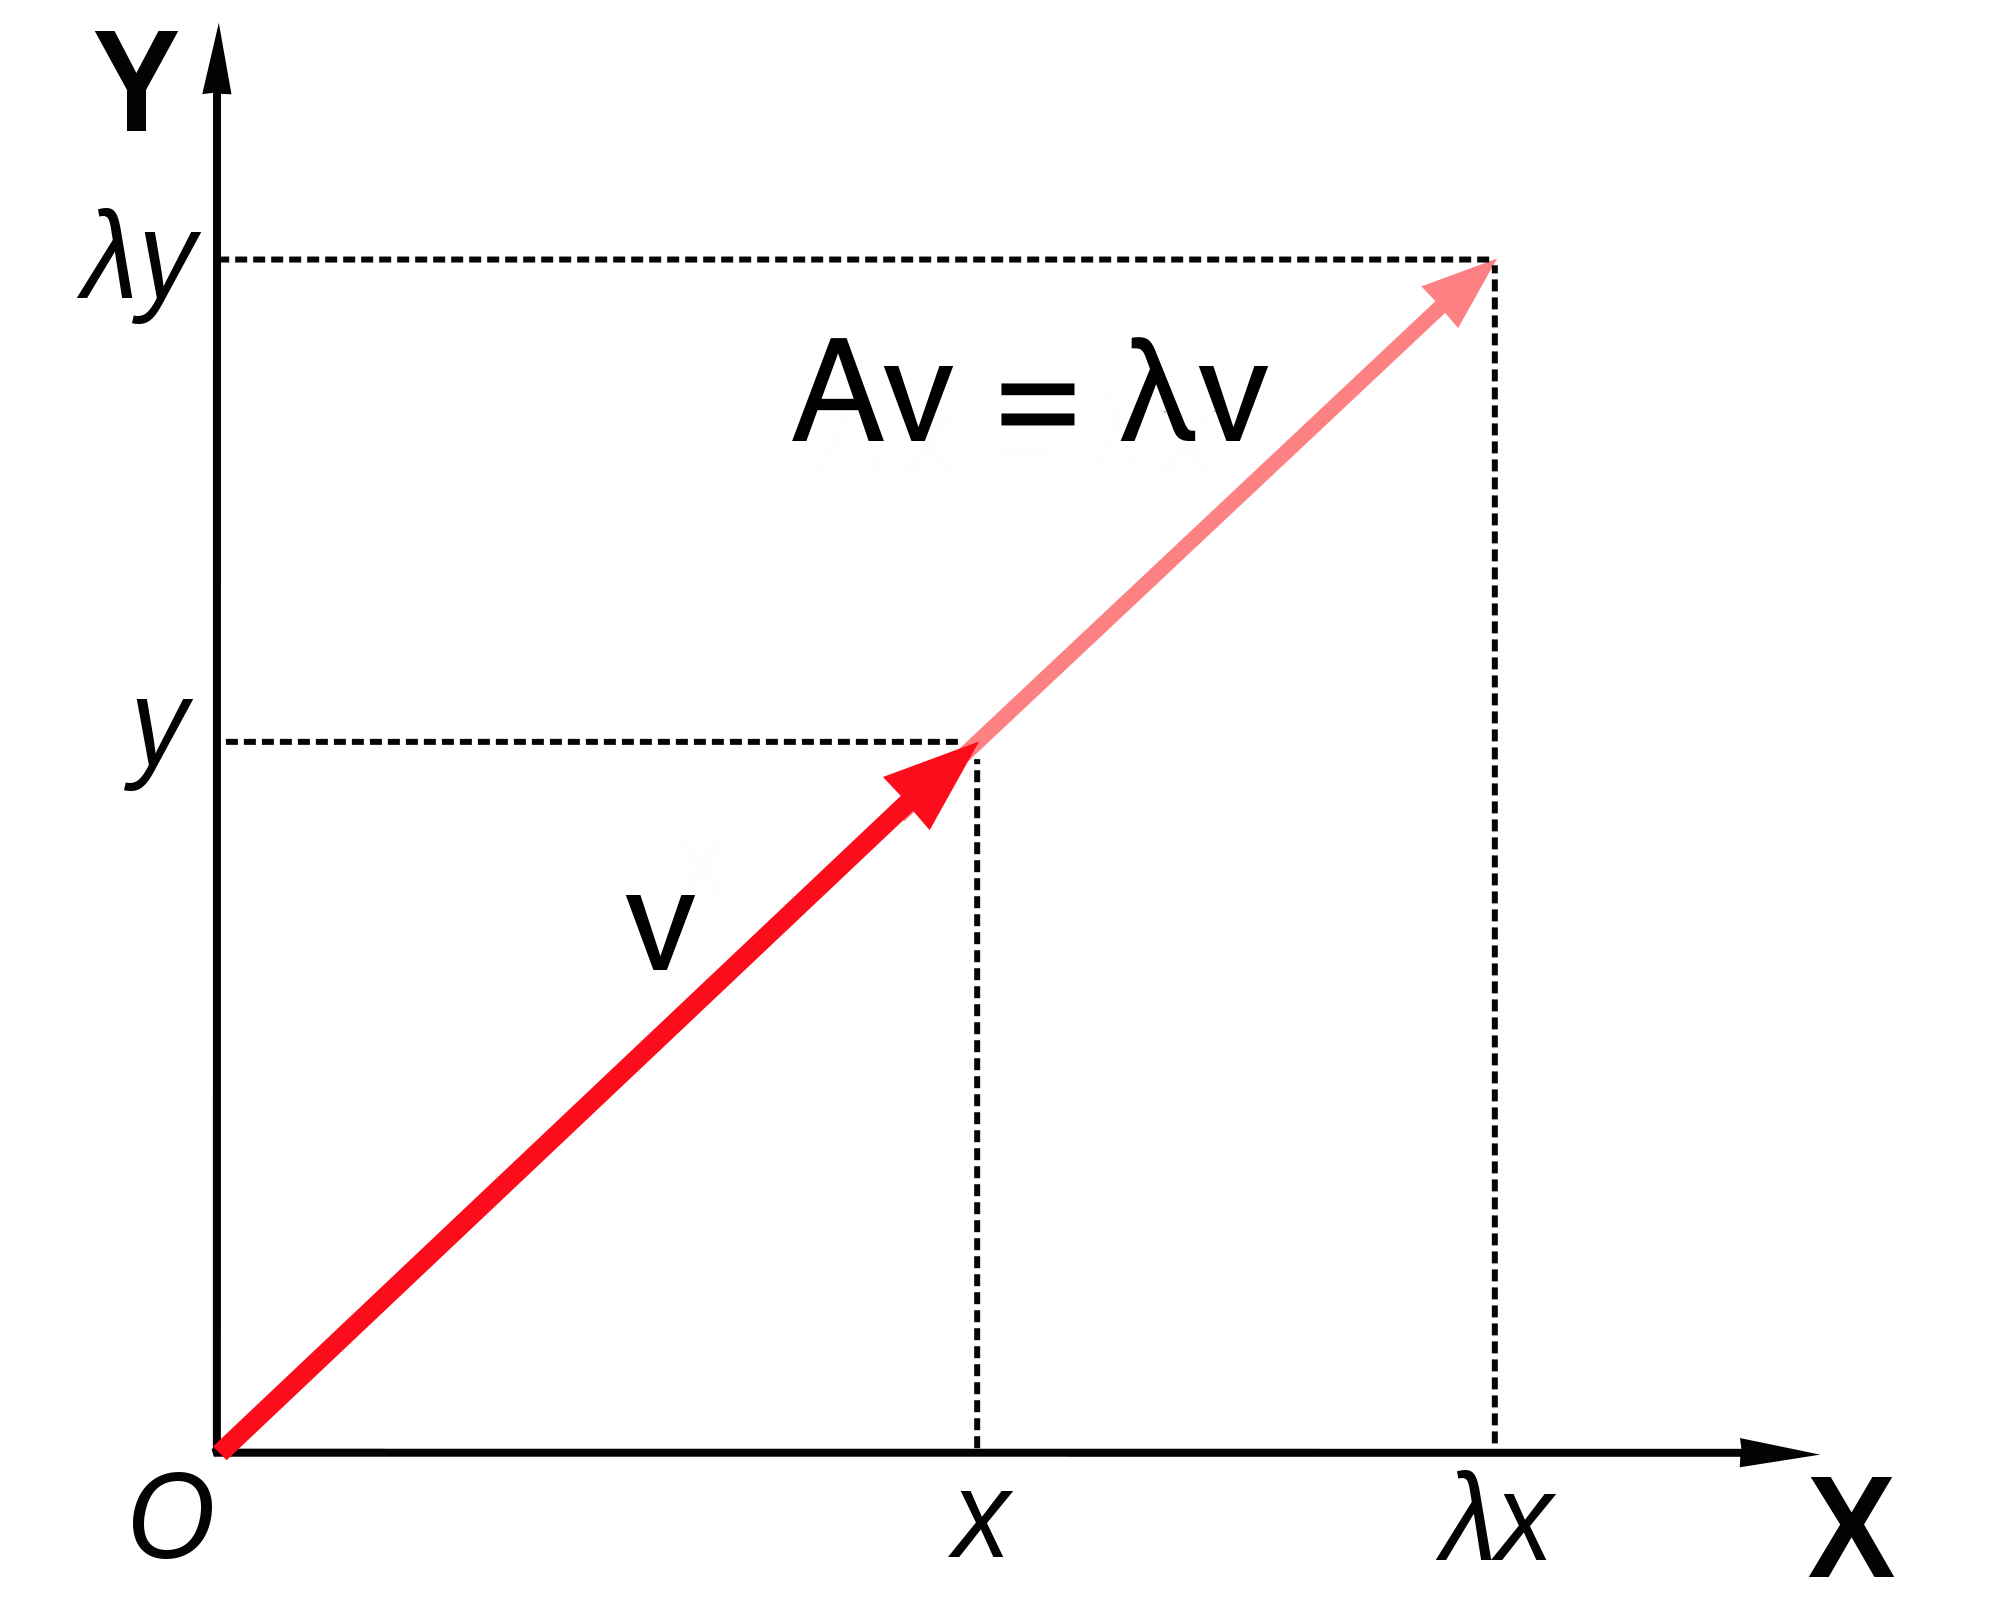
\includegraphics[keepaspectratio]{images/Eigenvalue_equation.png}}

}

\caption{Illustration of the geometry of a matrix \(A\) multiplying its
eigenvector \(v\), resulting in a vector in the same direction
\(\lambda v\)}

\end{figure}%

To summarize, eigenvalues and eigenvectors of a matrix are a set of
numbers and a set of vectors (up to scalar multiple) that describe the
action of the matrix as a multiplicative operator on vectors.
``Well-behaved'' square \(n \times n\) matrices have \(n\) distinct
eigenvalues and \(n\) eigenvectors pointing in distinct directions. In a
deep sense, the collection of eigenvectors and eigenvalues defines a
matrix \(A\), which is why an older name for them is characteristic
vectors and values.

\subsection{calculating eigenvalues}\label{calculating-eigenvalues}

Finding the eigenvalues and eigenvectors analytically, that is on paper,
is quite laborious even for 3 by 3 or 4 by 4 matrices and for larger
ones there is no analytical solution. In practice, the task is
outsourced to a computer, and MATLAB has a number of functions for this
purpose. Nevertheless, it is useful to go through the process in 2
dimensions in order to gain an understanding of what is involved. From
the definition of eigenvalues and eigenvectors, the condition can be
written in terms of the four elements of a 2 by 2 matrix:

\[
\left(\begin{array}{cc}a & b \\c & d\end{array}\right)\left(\begin{array}{c}v_1 \\ v_2 \end{array}\right) = \left(\begin{array}{c}av_1 +b v_2\\ cv_1+ dv_2 \end{array}\right) = \lambda \left(\begin{array}{c}v_1 \\ v_2 \end{array}\right)
\]

This is now a system of two linear algebraic equations, which we can
solve by substitution. First, let us solve for \(v_1\) in the first row,
to get \[v_1 = \frac{-bv_2}{a-\lambda}\] Then we substitute this into
the second equation and get:

\[
\frac{-bcv_2}{a-\lambda} +(d-\lambda)v_2 = 0
\]

Since \(v_2\) multiplies both terms, and is not necessarily zero, we
require that its multiplicative factor be zero. Doing a little algebra,
we obtain the following, known as the \emph{characteristic equation} of
the matrix:

\[
-bc +(a-\lambda)(d-\lambda) = \lambda^2-(a+d)\lambda +ad-bc = 0
\]

This equation can be simplified by using two quantities we defined at
the beginning of the section: the sum of the diagonal elements called
the trace \(\tau = a+d\), and the determinant \(\Delta = ad-bc\). The
quadratic equation has two solutions, dependent solely on \(\tau\) and
\(\Delta\):

\[
\lambda = \frac{\tau \pm \sqrt{\tau^2-4\Delta}}{2}
\]

This is the general expression for a 2 by 2 matrix, showing there are
two possible eigenvalues. Note that if \(\tau^2-4\Delta>0\), the
eigenvalues are real, if \(\tau^2-4\Delta<0\), they are complex (have
real and imaginary parts), and if \(\tau^2-4\Delta=0\), there is only
one eigenvalue. This situation is known as degenerate, because two
eigenvectors share the same eigenvalue.

\textbf{Example.} Let us take the same matrix we looked at in the
previous subsection:

\[
A = \left(\begin{array}{cc}2 & 1 \\ 2& 3\end{array}\right)
\]

The trace of this matrix is \(\tau = 2+3 =5\) and the determinant is
\(\Delta = 6 - 2 = 4\). Then by our formula, the eigenvalues are:

\[
\lambda = \frac{5 \pm \sqrt{5^2-4 \times 4}}{2}  =  \frac{5 \pm 3}{2}  = 4, 1
\]

These are the multiples we found in the example above, as expected. Of
course \texttt{R} has functions to calculate this instead of doing this
by hand:

\begin{Shaded}
\begin{Highlighting}[]
\NormalTok{A \textless{}{-} matrix(c(2, 2, 1, 3), nrow =2)}
\NormalTok{eigs \textless{}{-} eigen(A)}
\NormalTok{eigs$values}
\NormalTok{eigs$vectors}
\end{Highlighting}
\end{Shaded}

\textbf{Note:} a real-valued matrix can have complex eigenvalues and
eigenvectors, but whenever it acts on a real vector, the result is still
real. This is because the complex numbers cancel each others imaginary
parts.

\bookmarksetup{startatroot}

\chapter{Linear models}\label{linear-models}

Learn how to perform linear regression, how to make sure that the
assumptions of the model are not violated, and how to interpret the
results.

Note that we need a new library:

\begin{Shaded}
\begin{Highlighting}[]
\NormalTok{library(lindia) \# regression diagnostic in ggplot2}
\end{Highlighting}
\end{Shaded}

\section{Regression toward the mean}\label{regression-toward-the-mean}

Francis Galton (Darwin's half-cousin) was a biologist interested in
evolution, and one of the main proponents of eugenics (he coined the
term himself). To advance his research program, he set out to measure
several features in human populations, and started trying to explain the
variation he observed, incidentally becoming one of the founding fathers
of modern statistics.

In his ``Regression towards mediocrity in hereditary stature'' he showed
an interesting pattern: children of tall parents tended to be shorter
than their parents, while children of short parents tended to be taller
than their parents. He called this phenomenon ``regression toward
mediocrity'' (now called regression toward {[}to{]} the mean).

We're going to explore this phenomenon using Karl Pearson's (another
founding father of statistics) data from 1903, recording the height of
fathers and sons:

\begin{Shaded}
\begin{Highlighting}[]
\NormalTok{library(UsingR)}
\NormalTok{data("father.son")}
\NormalTok{pl \textless{}{-} ggplot(data = father.son) + aes(x = fheight, y = sheight) + geom\_point() + coord\_equal()}
\NormalTok{pl}
\end{Highlighting}
\end{Shaded}

Let's add the 1:1 line for comparison:

\begin{Shaded}
\begin{Highlighting}[]
\NormalTok{pl + geom\_abline(slope = 1, intercept = 0, linetype = 2, color = "red")}
\end{Highlighting}
\end{Shaded}

You can see that the sons tend to be taller than their fathers. Let's
see of how much:

\begin{Shaded}
\begin{Highlighting}[]
\NormalTok{mean(father.son$fheight)}
\NormalTok{mean(father.son$sheight)}
\NormalTok{\# difference}
\NormalTok{mean(father.son$sheight) {-} mean(father.son$fheight)}
\end{Highlighting}
\end{Shaded}

So let's add a line with an intercept of 1:

\begin{Shaded}
\begin{Highlighting}[]
\NormalTok{pl \textless{}{-} pl + geom\_abline(slope = 1, intercept = 1, linetype = 2, color = "blue")}
\NormalTok{pl}
\end{Highlighting}
\end{Shaded}

You can see that the line does not divide the cloud of points evenly:
even though tall fathers tend to produce tall sons, and short fathers
short sons, the sons of short fathers tend to be taller than their
fathers (for example, look at the sons of fathers less than 60 inches
tall), while the sons of tall fathers tend to be shorter than their
fathers (for example, the sons of fathers taller than 75 inches).

This phenomenon is called ``regression toward the mean'': when you take
two measurement on the same sample (or related samples, as here), if a
variable is extreme on its first measurement, it will tend to be closer
to the average on its second measurement; if it is extreme on its second
measurement, it will tend to have been closer to the average on its
first.

\begin{quote}
\textbf{Regression to the mean: dangers of interpretation}
\end{quote}

\begin{itemize}
\tightlist
\item
  A city sees an unusual growth of crime in a given neighborhood, and
  they decide to patrol the neighborhood more heavily. The next year,
  crime rates are close to normal. Was this due to heavy presence of
  police?
\item
  A teacher sees that scolding students who've had a very low score in a
  test makes them perform better in the next test. (But would praising
  those with unusually high scores lead to slacking off in the next
  test?)
\item
  A huge problem in science: effect sizes tend to decrease through time.
  Problem of selective reporting?
\end{itemize}

This phenomenon gave the name to one of the simplest statistical models:
the linear regression.

\section{Finding the best fitting line: Linear
Regression}\label{finding-the-best-fitting-line-linear-regression}

How can we explain the relationship between the height of the fathers
and those of their sons? One of the simplest models we can use is called
a ``Linear Model''. Basically, we want to express the height of the son
as a function of the height of the father:

\[
y_i = \beta_0 + \beta_1 x_i + \epsilon_i
\]

where \(y_i\) is the height of the son (\textbf{response variable}),
\(x_i\) is the height of the father (\textbf{explanatory variable}),
\(\beta_0\) and \(\beta_1\) are two numbers (intercept and slope of the
line) that do not vary within the population (these are the parameters
we want to fit). Finally, the term \(\epsilon_i\) measures the ``error''
we are making for the \(i^{th}\) son. For simplicity, we assume the
\(\epsilon_i \overset{\text{iid}}{\sim} \mathcal N(0, \sigma^2)\) (and
\(\sigma\) is therefore another parameter we want to fit).

When we have multiple explanatory variables (for example, if we had
recorded also the height of the mother, whether the son was born at full
term or premature, the average caloric intake for the family, etc.), we
speak of \textbf{Multiple Linear Regression}:

\[
y_i = \beta_0 + \sum_{k=1}^n \beta_k x_{ik} + \epsilon_i
\]

\subsection{Solving a linear model --- some linear
algebra}\label{solving-a-linear-model-some-linear-algebra}

In this section, we're going to look at the mechanics of linear
regression. Suppose that for simplicity we have a single explanatory
variable, then we can write the linear model in compact form as:

\[
\mathbf{Y} = \mathbf{X} \mathbf{\beta} + \mathbf{\epsilon}
\]

where:

\[
\mathbf{Y} = \begin{pmatrix} y_1\\ y_2\\ \vdots \\ y_n \end{pmatrix} \;\;\; 
\mathbf{X} = \begin{pmatrix} 1 & x_1\\ 1 & x_2\\ \vdots & \vdots \\ 1 & x_n \end{pmatrix}
 \;\;\; 
\mathbf{\beta} = \begin{pmatrix} \beta_0 \\ \beta_1\end{pmatrix} \;\;\; \mathbf{\epsilon} = \begin{pmatrix} \epsilon_1 \\ \epsilon_2 \\ \vdots \\ \epsilon_n \end{pmatrix}
\]

Solving the linear regression means finding the best-fitting
\(\beta_0\), \(\beta_1\) and \(\sigma\) (controlling the spread of the
distribution of the \(\epsilon_i\)). Our goal is to find the values of
\(\beta\) that minimize \(\sigma\) (meaning that the points fall closer
to the line). Rearranging:

\[
\sum_i \epsilon_i^2 = \sum_i (y_i - \beta_0 - \beta_1 x_i)^2 =  \Vert \mathbf{Y} - \mathbf{X} \mathbf{\beta} \Vert
\]

As such, we want to find the vector \(\beta\) that minimizes the norm
\(\Vert \mathbf{Y} - \mathbf{X} \mathbf{\beta} \Vert\). One can prove
that this is accomplished using:

\[
\hat{\mathbf{\beta}} = \left( \mathbf{X}^T \mathbf{X} \right)^{-1} \mathbf{X}^T \mathbf{Y}
\]

Where the matrix
\(\left( \mathbf{X}^T \mathbf{X} \right)^{-1} \mathbf{X}^T\) is known as
the (left) Moore-Penrose pseudo-inverse of \(\mathbf{X}\). Let's try to
do this in \texttt{R} (the ``hard'' way):

\begin{Shaded}
\begin{Highlighting}[]
\NormalTok{X \textless{}{-} cbind(1, father.son$fheight)}
\NormalTok{Y \textless{}{-} cbind(father.son$sheight)}
\NormalTok{best\_beta \textless{}{-} solve(t(X) \%*\% X) \%*\% t(X) \%*\% Y}
\NormalTok{best\_beta}
\end{Highlighting}
\end{Shaded}

We find that the best fitting line has an intercept of about 34 inches,
and a slope of 0.51. Of course, \texttt{R} can do this calculation for
you with just one command:

\begin{Shaded}
\begin{Highlighting}[]
\NormalTok{best\_beta\_easy \textless{}{-} lm(sheight \textasciitilde{} fheight, data = father.son)}
\NormalTok{best\_beta\_easy}
\end{Highlighting}
\end{Shaded}

But it feels good to know that this is not black magic! In fact,
plotting it on top of the data does not even require computing the
coefficients:

\begin{Shaded}
\begin{Highlighting}[]
\NormalTok{pl + geom\_smooth(method = "lm") \# lm stands for linear model}
\end{Highlighting}
\end{Shaded}

\subsection{Minimizing the sum of
squares}\label{minimizing-the-sum-of-squares}

What we just did is called ``ordinary least-squares'': we are trying to
minimize the distance from the data points to their projection on the
best-fitting line. We can compute the ``predicted'' heights as:

\[
\hat{\mathbf{Y}} = \mathbf{X}\hat{\mathbf{\beta}}
\]

Then, we're minimizing \(\Vert \mathbf{Y} - \hat{\mathbf{Y}}\Vert\). We
call \(\hat{\mathbf{\epsilon}} = \mathbf{Y} - \hat{\mathbf{Y}}\) the
vector of \textbf{residuals}. From this, we can estimate the final
parameter, \(\sigma\):

\[
\sigma = \sqrt{\frac{\sum_i \hat{\epsilon_i}^2}{n -  p}}
\]

where \(n\) is the number of data points, and \(p\) is the number of
parameters in \(\mathbf{\beta}\) (2 in this case); this measures the
number of \textbf{degrees of freedom}. Let's try to compute it:

\begin{Shaded}
\begin{Highlighting}[]
\NormalTok{degrees\_of\_freedom \textless{}{-} length(Y) {-} 2}
\NormalTok{degrees\_of\_freedom}
\NormalTok{epsilon\_hat \textless{}{-} X \%*\% best\_beta {-} Y}
\NormalTok{sigma \textless{}{-} sqrt(sum(epsilon\_hat\^{}2) / degrees\_of\_freedom)}
\NormalTok{sigma}
\end{Highlighting}
\end{Shaded}

In \texttt{R}, you will find this reported as the
\texttt{Residual\ standard\ error} when you call \texttt{summary} on
your model:

\begin{Shaded}
\begin{Highlighting}[]
\NormalTok{summary(best\_beta\_easy)}
\end{Highlighting}
\end{Shaded}

Finally, the \textbf{coefficient of determination} \(R^2\) is computed
as:

\[
R^2 = \frac{\sum_i (\hat{y}_i - \bar{y})^2}{\sum_i ({y}_i - \bar{y})^2}
\]

where \(\bar{y}\) is the mean of \(y_i\). If the regression has an
intercept, then the \(R^2\) can vary between 0 and 1, with values close
to 1 indicating a good fit to the data. Again, let's compute it the hard
way and then the easy way:

\begin{Shaded}
\begin{Highlighting}[]
\NormalTok{y\_bar \textless{}{-} mean(Y)}
\NormalTok{R\_2 \textless{}{-} sum((X \%*\% best\_beta {-} y\_bar)\^{}2) / sum((Y {-} y\_bar)\^{}2)}
\NormalTok{R\_2}
\end{Highlighting}
\end{Shaded}

\begin{Shaded}
\begin{Highlighting}[]
\NormalTok{\# look for Multiple R{-}squared:}
\NormalTok{summary(best\_beta\_easy)}
\end{Highlighting}
\end{Shaded}

\subsection{Assumptions of linear
regression}\label{assumptions-of-linear-regression}

In practice, when we are performing a linear regression, we are making a
number of assumptions about the data. Here are the main ones:

\begin{itemize}
\tightlist
\item
  Model structure: we assume that the process generating the data is
  linear.
\item
  Explanatory variable: we assume that this is measured without errors
  (!).
\item
  Residuals: we assume that residuals are i.i.d. Normal.
\item
  Strict exogeneity: the residuals should have conditional mean of 0.
\end{itemize}

\[
\mathbb E[\epsilon_i | x_i] = 0
\]

\begin{itemize}
\tightlist
\item
  No linear dependence: the columns of \(\mathbf{X}\) should be linearly
  independent.
\item
  Homoscedasticity: the variance of the residuals is independent of
  \(x_i\).
\end{itemize}

\[
\mathbb V[\epsilon_i | x_i] =  \sigma^2
\]

\begin{itemize}
\tightlist
\item
  Errors are uncorrelated between observations.
\end{itemize}

\[
\mathbb E[\epsilon_i \epsilon_j | x] = 0 \; \forall j \neq i
\]

\section{Linear regression in action}\label{linear-regression-in-action}

To perform a slightly more complicated linear regression, we take the
data from:

\begin{quote}
Piwowar HA, Day RS, Fridsma DB (2007)
\href{https://doi.org/10.1371/journal.pone.0000308}{Sharing detailed
research data is associated with increased citation rate}. PLoS ONE
2(3): e308.
\end{quote}

The authors set out to demonstrate that sharing data accompanying papers
tends to increase the number of citations received by the paper.

\begin{Shaded}
\begin{Highlighting}[]
\NormalTok{\# original URL }
\NormalTok{\# https://datadryad.org/stash/dataset/doi:10.5061/dryad.j2c4g}
\NormalTok{dat \textless{}{-} read\_csv("https://raw.githubusercontent.com/StefanoAllesina/BIOS\_26318/refs/heads/master/data/Piwowar\_2011.csv") }
\NormalTok{\# rename variables for easier handling}
\NormalTok{dat \textless{}{-} dat |\textgreater{} rename(IF = \textasciigrave{}Impact factor of journal\textasciigrave{}, }
\NormalTok{                      NCIT = \textasciigrave{}Number of Citations in first 24 months after publication\textasciigrave{}, }
\NormalTok{                      SHARE = \textasciigrave{}Is the microarray data publicly available\textasciigrave{}) |\textgreater{} }
\NormalTok{      dplyr::select(NCIT, IF, SHARE)}
\end{Highlighting}
\end{Shaded}

First, let's run a model in which the logarithm of the number of
citations + 1 is regressed against the ``Impact Factor'' of the journal
(which is a measure of ``prestige'' based on the average number of
citations per paper received):

\begin{Shaded}
\begin{Highlighting}[]
\NormalTok{my\_model \textless{}{-} lm(log(NCIT + 1) \textasciitilde{} log(IF + 1), data = dat)}
\NormalTok{summary(my\_model)}
\end{Highlighting}
\end{Shaded}

You can see that the higher the impact factor, the higher the number of
citations received (unsurprisingly!). Now let's add another variable,
detailing whether publicly available data accompany the paper:

\begin{Shaded}
\begin{Highlighting}[]
\NormalTok{my\_model2 \textless{}{-} lm(log(NCIT + 1) \textasciitilde{} log(IF + 1) + SHARE, data = dat)}
\NormalTok{summary(my\_model2)}
\end{Highlighting}
\end{Shaded}

We find that sharing data is associated with a larger number of
citations.

\section{A regression gone wild}\label{a-regression-gone-wild}

Even when the fit is good, and assumptions are met, one can still end up
with a fantastic blunder. To show this, we are going to repeat a study
published in \emph{Nature} (no less!) by Tatem \emph{et al}. You can
find the study \href{https://www.nature.com/articles/431525a}{here}.
Briefly, the Authors gathered data on the 100m sprint at the Olympics
from 1900 to 2004, for both men and women. We can do the same:

\begin{Shaded}
\begin{Highlighting}[]
\NormalTok{olympics \textless{}{-} read\_csv("https://raw.githubusercontent.com/StefanoAllesina/BIOS\_26318/refs/heads/master/data/100m\_dash.csv")}
\end{Highlighting}
\end{Shaded}

Then, they fitted a linear regression through the points, for both men
and women. So far, so good:

\begin{Shaded}
\begin{Highlighting}[]
\NormalTok{ggplot(data = olympics |\textgreater{} filter(Year \textgreater{} 1899, Year \textless{} 2005)) + }
\NormalTok{  aes(x = Year, y = Result, colour = Gender) + }
\NormalTok{  geom\_point() + geom\_smooth(method = "lm")}
\end{Highlighting}
\end{Shaded}

The fit is quite good:

\begin{Shaded}
\begin{Highlighting}[]
\NormalTok{summary(lm(Result \textasciitilde{} Year*Gender,}
\NormalTok{  data = olympics |\textgreater{} filter(Year \textgreater{} 1899, Year \textless{} 2005)))}
\end{Highlighting}
\end{Shaded}

An \(R^2\) of 0.93, the pinnacle of a good linear regression. Now
however, comes the problem. The Authors noticed that the times recorded
for women are falling faster than those for men, meaning that the gender
gap is reducing. Will it ever disappear? Just extend the regression and
project forward:

\begin{Shaded}
\begin{Highlighting}[]
\NormalTok{ggplot(data = olympics |\textgreater{} filter(Year \textgreater{} 1899, Year \textless{} 2005)) + }
\NormalTok{  aes(x = Year, y = Result, colour = Gender) + }
\NormalTok{  geom\_point() + geom\_smooth(method = "lm", fullrange = TRUE, se = FALSE) +}
\NormalTok{  xlim(c(1890, 2200)) + ylim(c(0, 13))}
\end{Highlighting}
\end{Shaded}

You can see that the lines are touching in sometimes before 2200! Then
women will overrun men.

There are a number of things that are wrong with this result. First, by
the same logic, computers will soon go faster than the speed of light,
the number of people on planet Earth will be in the hundreds of
billions, and the price of sequencing will drop so much that we will be
paid instead of paying to get our samples sequenced\ldots{}

Second, if we extend backwards, rather than forward, we would find that
Roman women would take more than a minute to run 100m (possibly, because
of the uncomfortable tunics and sandals\ldots).

\begin{Shaded}
\begin{Highlighting}[]
\NormalTok{ggplot(data = olympics |\textgreater{} filter(Year \textgreater{} 1899, Year \textless{} 2005)) + }
\NormalTok{  aes(x = Year, y = Result, colour = Gender) + }
\NormalTok{  geom\_point() + geom\_smooth(method = "lm", fullrange = TRUE, se = FALSE) +}
\NormalTok{  xlim(c({-}2000, 2200)) + ylim(c(0, 75))}
\end{Highlighting}
\end{Shaded}

As Neil Bohr allegedly said (but this is disputed), ``Prediction is very
difficult, especially about the future''. The fact is that any
non-linear curve looks quite linear if we are only considering a small
range of values on the x-axis. To prove this point, let's add the data
from 2004 to today:

\begin{Shaded}
\begin{Highlighting}[]
\NormalTok{ggplot(data = olympics |\textgreater{} filter(Year \textgreater{} 1899)) + }
\NormalTok{  aes(x = Year, y = Result, colour = Gender) + }
\NormalTok{  geom\_point() + geom\_smooth(method = "lm", fullrange = TRUE, se = FALSE) +}
\NormalTok{  xlim(c(1890, 2400)) + ylim(c(0, 13))}
\end{Highlighting}
\end{Shaded}

You can see that the process has already slowed down: now it would take
an extra century before the ``momentous sprint''.

So many things were wrong with this short paper, that \emph{Nature} was
showered with replies. My favorite is from a Cambridge statistician (the
Authors were from Oxford, ça va sans dire); it is perfectly short and
venomous---a good candidate for the Nobel prize in Literature!

\begin{quote}
Sir --- A. J. Tatem and colleagues calculate that women may outsprint
men by the middle of the twenty-second century (Nature 431, 525; 2004).
They omit to mention, however, that (according to their analysis) a far
more interesting race should occur in about 2636, when times of less
than zero seconds will be recorded. In the intervening 600 years, the
authors may wish to address the obvious challenges raised for both
time-keeping and the teaching of basic statistics. --- Kenneth Rice
\end{quote}

\section{More advanced topics}\label{more-advanced-topics}

\subsection{Categorical variables in linear
models}\label{categorical-variables-in-linear-models}

In the example above, we have built the model:

\[
 \log(\text{NCIT} + 1) = \beta_0 + \beta_1 (\log(\text{IF} + 1))_i + \beta_2 (\text{SHARE})_i + \epsilon_i
\]

In this case, the variable SHARE takes values of 1 or 0. As such, when
the data were not shared (SHARE = 0) the model reduces to the previous
one, in which \(\beta_2\) was absent. The coefficient \(\beta_2\)
measures the increase in the log of citation count when data are shared.

The same approach can be taken whenever you have categorical values:
\texttt{R} will automatically create \textbf{dummy variables} each
encoding whether the ith data point belongs to a particular category.
For example, suppose you want to predict the height of a child based on
the height of the father, and that you also collected the gender, in
three categories: \texttt{F} for female, \texttt{M} for male, \texttt{U}
for unknown. Then you could use this information to build the model:

\[
 \text{height}_i = \beta_0 + \beta_1 \text{(height of father)}_i + \beta_2 (\text{gender is M})_i + \beta_3 (\text{gender is U})_i + \epsilon_i
\]

where the variable \texttt{gender\ is\ M} takes value 1 when the gender
is \texttt{M} and 0 otherwise, and \texttt{gender\ is\ U} takes value 1
when the gender is unknown and 0 otherwise. As such, when the gender is
\texttt{F} both variables will be zero, and \(\beta_2\) and \(\beta_3\)
measure the increase (or decrease) in height for males and those with
unspecified gender, respectively. While \texttt{R} does this for you
automatically, understanding what is going on ``under the hood'' is
essential for interpreting the results.

\subsection{Interactions in linear
models}\label{interactions-in-linear-models}

Sometimes we think that our explanatory variables could ``interact''.
For example, suppose you want to predict the BMI of people. What we have
available is the average caloric intake, the height, gender, and whether
they are vegetarian, vegan, or omnivores. A simple model could be:

\[
\text{BMI}_i = \beta_0 + \beta_h \text{height}_i + \beta_c \text{calories}_i + \beta_g \text{gender}_i + \epsilon_i
\]

We could add the type of diet as a factor:

\[
\text{BMI}_i = \beta_0 + \beta_h \text{height}_i + \beta_c \text{calories}_i + \beta_g \text{gender}_i + \beta_d \text{diet}_i + \epsilon_i
\]

However, suppose that we believe the type of diet to affect
differentially men and women. Then, we would like to create an
``interaction'' (e.g., paleo-female, vegan-male):

\[
\text{BMI}_i = \beta_0 + \beta_h \text{height}_i + \beta_c \text{calories}_i + \beta_g \text{gender}_i + \beta_d \text{diet}_i + \beta_{gd} \text{gender:diet}_i + \epsilon_i
\]

where the colon signals ``interaction''. In \texttt{R}, this would be
coded as
\texttt{lm(BMI\ \textasciitilde{}\ height\ +\ calories\ +\ gender\ *\ diet)}.
A simpler model is one in which we only account for the
\texttt{gender:diet} interaction, but not for the separate effects of
gender and diet:

\[
\text{BMI}_i = \beta_0 + \beta_h \text{height}_i + \beta_c \text{calories}_i + \beta_{gd}\text{gender:diet}_i + \epsilon_i
\]

which in \texttt{R} can be coded as
\texttt{lm(BMI\ \textasciitilde{}\ height\ +\ calories\ +\ gender:diet)}.
Finally, for some models you believe the intercept should be 0 (note
that this makes the \(R^2\) statistics uninterpretable!). In \texttt{R},
just put \texttt{-1} at the end of the definition of the model (e.g.,
\texttt{lm(BMI\ \textasciitilde{}\ height\ +\ calories\ +\ gender:diet\ -\ 1)}).

\subsection{Regression diagnostics}\label{regression-diagnostics}

Now that we know the mechanics of linear regression, we turn to
diagnostics: how can we make sure that the model fits the data ``well''?
We start by analyzing a data set assembled by Anscombe (\emph{The
American Statistician}, 1973)

\begin{Shaded}
\begin{Highlighting}[]
\NormalTok{dat \textless{}{-} read\_csv("https://raw.githubusercontent.com/StefanoAllesina/BIOS\_26318/refs/heads/master/data/Anscombe\_1973.csv")}
\end{Highlighting}
\end{Shaded}

The file comprised four data sets. We perform a linear regression using
each data set separately:

\begin{Shaded}
\begin{Highlighting}[]
\NormalTok{lm(Y \textasciitilde{} X, data = dat |\textgreater{} filter(Data\_set == "Data\_1"))}
\NormalTok{lm(Y \textasciitilde{} X, data = dat |\textgreater{} filter(Data\_set == "Data\_2"))}
\NormalTok{lm(Y \textasciitilde{} X, data = dat |\textgreater{} filter(Data\_set == "Data\_3"))}
\NormalTok{lm(Y \textasciitilde{} X, data = dat |\textgreater{} filter(Data\_set == "Data\_4"))}
\end{Highlighting}
\end{Shaded}

As you can see, each data set is best fit by the same line, with
intercept 3 and slope \(\frac{1}{2}\). Plotting the data, however, shows
that the situation is more complicated:

\begin{Shaded}
\begin{Highlighting}[]
\NormalTok{ggplot(data = dat) + aes(x = X, y = Y, colour = Data\_set) + }
\NormalTok{  geom\_point() + geom\_smooth(method = "lm", se = FALSE) + }
\NormalTok{  facet\_wrap(\textasciitilde{}Data\_set)}
\end{Highlighting}
\end{Shaded}

\texttt{Data\_1} is fitted quite well; \texttt{Data\_2} shows a marked
nonlinearity; all points but one in \texttt{Data\_3} are on the same
line, but a single \textbf{outlier} shifts the line considerably;
finally, in \texttt{Data\_4} a single point is responsible for the
fitting line: all other values of \texttt{X} are exactly the same.
Inspecting the graphs, we would conclude that we can trust our model
only in the first case. When you are performing a multiple regression,
however, it is hard to see whether we're in case 1, or one of the other
cases. \texttt{R} provides a number of diagnostic tools which can help
you decide whether the fit to the data is good.

\subsection{Plotting the residuals}\label{plotting-the-residuals}

The first thing you want to do is to plot the residuals as a function of
the fitted values. This plot should make it apparent whether the data
was linear or not. The package \texttt{lindia} (linear regression
diagnostics) makes it easy to produce this type of plot using
\texttt{ggplot2}:

\begin{Shaded}
\begin{Highlighting}[]
\NormalTok{gg\_resfitted(lm(Y \textasciitilde{} X, data = dat |\textgreater{} filter(Data\_set == "Data\_1"))) + geom\_smooth(method = "loess")}
\end{Highlighting}
\end{Shaded}

What you are looking for is an approximately flat line, meaning that the
residuals are approximately normally distributed with mean zero for each
fitted value. This is not the case in the other data sets:

\begin{Shaded}
\begin{Highlighting}[]
\NormalTok{gg\_resfitted(lm(Y \textasciitilde{} X, data = dat |\textgreater{} }
\NormalTok{                  filter(Data\_set == "Data\_2"))) + }
\NormalTok{  geom\_smooth(method = "loess")}
\NormalTok{gg\_resfitted(lm(Y \textasciitilde{} X, data = dat |\textgreater{} }
\NormalTok{                  filter(Data\_set == "Data\_3"))) + }
\NormalTok{  geom\_smooth(method = "loess")}
\NormalTok{gg\_resfitted(lm(Y \textasciitilde{} X, data = dat |\textgreater{} }
\NormalTok{                  filter(Data\_set == "Data\_4"))) + }
\NormalTok{  geom\_smooth(method = "loess")}
\end{Highlighting}
\end{Shaded}

\subsection{Q-Q Plot}\label{q-q-plot}

We can take this further, and test whether the residuals follow a normal
distribution. In particular, we can estimate the density of the
residuals, and plot it against the density of a normal distribution:

\begin{Shaded}
\begin{Highlighting}[]
\NormalTok{gg\_qqplot(lm(Y \textasciitilde{} X, data = dat |\textgreater{} filter(Data\_set == "Data\_1")))}
\NormalTok{gg\_qqplot(lm(Y \textasciitilde{} X, data = dat |\textgreater{} filter(Data\_set == "Data\_2")))}
\NormalTok{gg\_qqplot(lm(Y \textasciitilde{} X, data = dat |\textgreater{} filter(Data\_set == "Data\_3")))}
\NormalTok{gg\_qqplot(lm(Y \textasciitilde{} X, data = dat |\textgreater{} filter(Data\_set == "Data\_4")))}
\end{Highlighting}
\end{Shaded}

Here, you are looking for a good match to the 1:1 line; outliers will be
found far from the line (e.g., case 3).

\subsection{Cook's distance}\label{cooks-distance}

Another way to detect outliers is to compute the Cook's distance for
every point. Briefly, this statistic measures the effect on the
regression we would obtain if we were to remove a point.

\begin{Shaded}
\begin{Highlighting}[]
\NormalTok{gg\_cooksd(lm(Y \textasciitilde{} X, data = dat |\textgreater{} filter(Data\_set == "Data\_1")))}
\NormalTok{gg\_cooksd(lm(Y \textasciitilde{} X, data = dat |\textgreater{} filter(Data\_set == "Data\_2")))}
\NormalTok{gg\_cooksd(lm(Y \textasciitilde{} X, data = dat |\textgreater{} filter(Data\_set == "Data\_3")))}
\NormalTok{gg\_cooksd(lm(Y \textasciitilde{} X, data = dat |\textgreater{} filter(Data\_set == "Data\_4")))}
\end{Highlighting}
\end{Shaded}

\subsection{Leverage}\label{leverage}

Points that strongly influence the regression are said to have much
``leverage'':

\begin{Shaded}
\begin{Highlighting}[]
\NormalTok{gg\_resleverage(lm(Y \textasciitilde{} X, data = dat |\textgreater{} filter(Data\_set == "Data\_1")))}
\NormalTok{gg\_resleverage(lm(Y \textasciitilde{} X, data = dat |\textgreater{} filter(Data\_set == "Data\_2")))}
\NormalTok{gg\_resleverage(lm(Y \textasciitilde{} X, data = dat |\textgreater{} filter(Data\_set == "Data\_3")))}
\NormalTok{gg\_resleverage(lm(Y \textasciitilde{} X, data = dat |\textgreater{} filter(Data\_set == "Data\_4")))}
\end{Highlighting}
\end{Shaded}

\subsection{Running all diagnostics}\label{running-all-diagnostics}

These are but a few of the diagnostics available. To run all diagnostics
on a given model, call

\begin{Shaded}
\begin{Highlighting}[]
\NormalTok{gg\_diagnose(lm(Y \textasciitilde{} X, data = dat |\textgreater{} filter(Data\_set == "Data\_2")))}
\end{Highlighting}
\end{Shaded}

\section{Transforming the data}\label{transforming-the-data}

Often, one needs to transform the data before running a linear
regression, in order to fulfill the assumptions. We're going to look at
the salary of professors at the University of California to show how
this is done.

\begin{Shaded}
\begin{Highlighting}[]
\NormalTok{\# read the data}
\NormalTok{\# Original URL}
\NormalTok{dt \textless{}{-} read\_csv("https://raw.githubusercontent.com/dailybruin/uc{-}salaries/master/data/uc\_salaries.csv", }
\NormalTok{               col\_names = c("first\_name", "last\_name", "title", "a", "pay", "loc", "year", "b", "c", "d")) |\textgreater{} }
\NormalTok{      dplyr::select(first\_name, last\_name, title, loc, pay)}
\NormalTok{\# get only profs}
\NormalTok{dt \textless{}{-} dt |\textgreater{} filter(title \%in\% c("PROF{-}AY", "ASSOC PROF{-}AY", "ASST PROF{-}AY", }
\NormalTok{                                 "PROF{-}AY{-}B/E/E", "PROF{-}HCOMP", "ASST PROF{-}AY{-}B/E/E", }
\NormalTok{                                 "ASSOC PROF{-}AY{-}B/E/E", "ASSOC PROF{-}HCOMP", "ASST PROF{-}HCOMP"))}
\NormalTok{\# remove those making less than 30k (probably there only for a period)}
\NormalTok{dt \textless{}{-} dt |\textgreater{} filter(pay \textgreater{} 30000)}
\NormalTok{dt}
\end{Highlighting}
\end{Shaded}

The distribution of salaries is very skewed --- it looks like a
log-normal distribution:

\begin{Shaded}
\begin{Highlighting}[]
\NormalTok{dt |\textgreater{} ggplot() + aes(x = pay) + geom\_histogram(binwidth = 10000)}
\end{Highlighting}
\end{Shaded}

If we set consider the log of pay, we get closer to a normal:

\begin{Shaded}
\begin{Highlighting}[]
\NormalTok{dt |\textgreater{} ggplot() + aes(x = log2(pay)) + geom\_histogram(binwidth = 0.5)}
\end{Highlighting}
\end{Shaded}

We can try to explain the pay as a combination of title and location:

\begin{Shaded}
\begin{Highlighting}[]
\NormalTok{unscaled \textless{}{-} lm(pay \textasciitilde{} title + loc, data = dt)}
\NormalTok{summary(unscaled)}
\NormalTok{gg\_diagnose(lm(pay \textasciitilde{} title + loc, data = dt))}
\end{Highlighting}
\end{Shaded}

To note: Berkeley has been taken as the baseline location. Similarly,
\texttt{ASSOC-PROF\ AY} has been taken as the baseline title.

The Q-Q plot shows that this is a terrible model! Now let's try with the
transformed data:

\begin{Shaded}
\begin{Highlighting}[]
\NormalTok{scaled \textless{}{-} lm(log2(pay) \textasciitilde{} title + loc, data = dt)}
\NormalTok{summary(scaled)}
\NormalTok{gg\_diagnose(lm(log2(pay) \textasciitilde{} title + loc, data = dt))}
\end{Highlighting}
\end{Shaded}

Much better! Remember to inspect your explanatory and response
variables. Ideally, you want the response to be normally distributed.
Sometimes one or many covariates can have a nonlinear relationship with
the response variable, and you should transform them prior to analysis.

\bookmarksetup{startatroot}

\chapter{ANOVA}\label{anova}

\section{Analysis of variance}\label{analysis-of-variance}

ANOVA is a method for testing the hypothesis that there is no difference
in means of subsets of measurements grouped by factors. Essentially,
this is a generalization of linear regression to categorical explanatory
variables instead of numeric variables, and it is based on very similar
assumptions.

ANOVA perform at its best when we have a particular experimental design:
a) we divide the population into groups of equal size (\textbf{balanced
design}); b) we assign ``treatments'' to the subjects at random
(\textbf{randomized design}); in case of multiple treatment
combinations, we perform an experiment for each combination
(\textbf{factorial design}); in most cases, we have a ``null'' treatment
(e.g., placebo).

We speak of \textbf{one-way ANOVA} when there is a single axis of
variation to our treatment (e.g., no intervention, option A, option B),
\textbf{two-way ANOVA} when we apply two treatments for each group
(e.g., no treatment, Ab, AB, aB), and so forth. Extensions include
ANCOVA (ANalysis of COVAriance) and MANOVA (Multivariate ANalysis Of
VAriance).

For example, we want to test whether a COVID vaccine protects against
infection. We can assign at random a population of volunteers to two
classes (vaccine/placebo) and contrast the number of people who got sick
within 3 months from treatment in the two classes. Of course, we can
simply perform a \emph{t}-test. But what if we assign people to
different classes (e.g., M/F, under/over 65 y/o), and want to contrast
the mean infection rate across all classes?

\subsection{ANOVA assumptions}\label{anova-assumptions}

ANOVA tests whether samples are taken from distributions with the same
mean:

\begin{itemize}
\tightlist
\item
  Null hypothesis: the means of the different groups are the same.
\item
  Alternative hypothesis: \textbf{At least one sample mean} is not equal
  to the others.
\end{itemize}

Let \(Y\) indicate the response variable, and study the simplest case of
one-way ANOVA. We have divided the samples in \(k\) classes of size
\(J_1, \ldots, J_k\) such that \(n=\sum_i J_i\). We write an equation
for \(Y_{ij}\) (the \(j\)th observation in group \(i\)):

\[
Y_{ij} = \mu + \alpha_i + \epsilon_{ij}
\]

where \(\mu\) is the \textbf{overall mean}; \(\mu + \alpha_i\) is the
mean of group \(i\)---we can always choose the parameters such that
\(\sum_i \alpha_i = 0\); and, finally, \(\epsilon_{ij}\) is the
deviation from the group mean. Practically, we are testing whether at
least one of the \(\alpha_i \neq 0\).

Note that we are making the same assumptions as for linear regression:

\begin{itemize}
\tightlist
\item
  The observations are obtained independently (and randomly) from the
  population defined by the factor levels (groups)
\item
  The measurements for each factor level are independent and normally
  distributed
\item
  These normal distributions have the same variance
\end{itemize}

\subsection{How one-way ANOVA works}\label{how-one-way-anova-works}

We have \(k\) groups, and define the overall mean
\(\bar{y} = \sum_i \sum_j Y_{ij} / J_{i}\), where \(J_i\) is the sample
size for group \(i\). Then the \textbf{total sum of squared deviations}
(SSD) is simply:

\[
SSD = \sum_{i = 1}^k \sum_{j = 1}^{J_{i}} \left(Y_{ij} - \bar{y}\right)^2
\]

and the associated degrees of freedom \(n-1\). We car rewrite this as:

\[
SSD = \sum_{i = 1}^k J_{i} \left(\bar{y}_i - \bar{y} \right)^2 + \sum_{j = 1}^{J_{i}} \left(Y_{ij} - \bar{y}_i \right)^2
\]

where now \(\bar{y}_i\) is the mean for the samples in treatment
(factor, group) \(i\). We call the first term in the r.h.s. the
\textbf{between treatment sum of squares} (SST) and the second term the
\textbf{within treatment (or residual) ssq} (SSE). As such
\(SSD = SST + SSE\). Similarly, we can decompose SSD as:

\[
SSD = \sum_{j = 1}^{J_{i}} Y_{ij}^2 - n \bar{y}^2 = TSS - SSA
\] where now TSS is the \textbf{total sum of squares} and SSA is the
\textbf{sum of squares due to the average}. Combining the two equations,
we can rewrite TSS as the sum of three components:

\[
TSS = SSA + SST + SSE
\]

Note that the degrees of freedom associated with each term are \(1\),
\(k-1\) and \(n-k\), respectively. What remains to be proved is how to
conduct inference.

\section{Inference in one-way ANOVA}\label{inference-in-one-way-anova}

If the null hypothesis were true, then we would expect the
between-treatment ``variance'' SST, divided by the degrees of freedom
(\(k-1\)) to be the same as the within-treatment ``variance'' divided by
\(n-k\).

Let's look at this hypothesis more closely. If the null hypothesis were
true, then \(SST\) would be the sum of the squares of independent,
normally distributed random variables with mean zero and variance
\(\sigma^2\). If you remember, the distribution of:

\[
Q = \sum_{i=1}^d Z_i^2 \sim \chi^2(d)
\]

is called the \(\chi^2\) distribution with \(d\) degrees of freedom.
Then, under the null hypothesis, \(SST \sim \chi^2(k-1)\) Similarly,
\(SSE \sim \chi^2(n-k)\). Taking the ratio (having normalized using the
degrees of freedom), we obtain:

\[
\frac{SST}{k-1} \frac{n-k}{SSE} = \frac{MST}{MSE} \sim F(k-1, n-k)
\] where \(F\) is the \textbf{F-distribution} (in \texttt{R}, you can
sample from this distribution using \texttt{df(x,\ deg1,\ deg2)}).

\subsection{Example of comparing
diets}\label{example-of-comparing-diets}

For example, the following data contains measurements of weights of
individuals before starting a diet, after 6 weeks of dieting, the type
of diet (1, 2, 3), and other variables.

\begin{Shaded}
\begin{Highlighting}[]
\NormalTok{\# Original URL: "https://www.sheffield.ac.uk/polopoly\_fs/1.570199!/file/stcp{-}Rdataset{-}Diet.csv"}
\NormalTok{diet \textless{}{-} read\_csv("https://raw.githubusercontent.com/StefanoAllesina/BIOS\_26318/refs/heads/master/data/Diet.csv") }
\NormalTok{diet \textless{}{-} diet |\textgreater{} mutate(weight.loss = pre.weight {-} weight6weeks) }
\NormalTok{glimpse(diet)}
\NormalTok{\# make diet into factors}
\NormalTok{diet \textless{}{-} diet |\textgreater{} mutate(Diet = factor(Diet))}
\end{Highlighting}
\end{Shaded}

Write a script below using ggplot to generate boxplots for the weights
after three different diets.

\begin{Shaded}
\begin{Highlighting}[]
\NormalTok{diet |\textgreater{} ggplot() + }
\NormalTok{  aes(y = weight.loss, }
\NormalTok{      x = Diet, }
\NormalTok{      fill = Diet) + }
\NormalTok{  geom\_boxplot()}
\end{Highlighting}
\end{Shaded}

We can see that there weight loss outcomes vary for each diet, but diet
3 seems to produce a larger effect on average. But is the difference
between the means/medians actually due to the diet, or could it have
been produced by sampling from the same distribution, given that we see
substantial variation within each diet group?

Here is the result of running ANOVA on the given data set:

\begin{Shaded}
\begin{Highlighting}[]
\NormalTok{diet\_anova  \textless{}{-}  aov(weight.loss \textasciitilde{} Diet, data=diet) \# note that this looks like lm!}
\NormalTok{summary(diet\_anova)}
\NormalTok{print(diet\_anova)}
\end{Highlighting}
\end{Shaded}

\subsection{Comparison of theory and ANOVA
output}\label{comparison-of-theory-and-anova-output}

Let's compare this with the calculations from the data set:

\begin{Shaded}
\begin{Highlighting}[]
\NormalTok{\# 1) compute the overall mean}
\NormalTok{bar\_y \textless{}{-} diet |\textgreater{} }
\NormalTok{  summarise(bar\_y = mean(weight.loss)) |\textgreater{} }
\NormalTok{  as.numeric()}
\NormalTok{\# 2) compute means by diet and sample size by diet}
\NormalTok{bar\_y\_i \textless{}{-} diet |\textgreater{} }
\NormalTok{  group\_by(Diet) |\textgreater{} }
\NormalTok{  summarise(bar\_y\_i = mean(weight.loss),}
\NormalTok{            J\_i = n())}
\NormalTok{\#(NB: almost balanced!)}

\NormalTok{\# 3) compute degrees of freedom}
\NormalTok{n \textless{}{-} nrow(diet)}
\NormalTok{k \textless{}{-} nrow(diet |\textgreater{} dplyr::select(Diet) |\textgreater{} distinct())}
\NormalTok{deg\_freedom \textless{}{-} c(1, k {-} 1, n {-} k)}
\NormalTok{\# 4) compute SSA, SST and SSE}
\NormalTok{SSA \textless{}{-} n * bar\_y\^{}2}
\NormalTok{SST \textless{}{-} bar\_y\_i |\textgreater{} }
\NormalTok{  mutate(tmp = J\_i * (bar\_y\_i {-} bar\_y)\^{}2) |\textgreater{} }
\NormalTok{  summarise(sst = sum(tmp)) |\textgreater{} }
\NormalTok{  as.numeric()}
\NormalTok{SSE \textless{}{-} diet |\textgreater{} }
\NormalTok{  inner\_join(bar\_y\_i, by = "Diet") |\textgreater{} }
\NormalTok{  mutate(tmp = (weight.loss {-} bar\_y\_i)\^{}2) |\textgreater{} }
\NormalTok{  summarise(sse = sum(tmp)) |\textgreater{} }
\NormalTok{  as.numeric()}
\NormalTok{\# 5) show that TSS = SSA + SST + SSE}
\NormalTok{TSS \textless{}{-} diet |\textgreater{} }
\NormalTok{  summarise(tss = sum(weight.loss\^{}2)) |\textgreater{} }
\NormalTok{  as.numeric()}
\NormalTok{print(c(TSS, SSA + SST + SSE))}
\end{Highlighting}
\end{Shaded}

Now that we have all the numbers in place, we can compute our
F-statistics, and the associated p-value:

\begin{Shaded}
\begin{Highlighting}[]
\NormalTok{Fs \textless{}{-} (SST / (deg\_freedom[2])) / (SSE / (deg\_freedom[3]))}
\NormalTok{pval \textless{}{-} 1 {-} pf(Fs, deg\_freedom[2], deg\_freedom[3])}
\end{Highlighting}
\end{Shaded}

Contrast these with the output of \texttt{aov}:

\begin{Shaded}
\begin{Highlighting}[]
\NormalTok{print(deg\_freedom[{-}1])}
\NormalTok{print(c(SST, SSE))}
\NormalTok{print(c(Fs, pval))}
\NormalTok{print(summary(aov(weight.loss \textasciitilde{} Diet, data = diet)))}
\end{Highlighting}
\end{Shaded}

At first glance, this process is not the same as fitting parameters for
linear regression, but it is based on exactly the same assumptions:
additive noise and additive effect of the factors, with the only
difference being that factors are not numeric, so the effect of each one
is added separately. One can run linear regression and calculate
coefficients that are identical to the mean and the differences between
means computed by ANOVA (and note the p-values too!)

\begin{Shaded}
\begin{Highlighting}[]
\NormalTok{diet.lm \textless{}{-} lm(weight.loss \textasciitilde{} Diet, data=diet)}
\NormalTok{summary(diet.lm)}
\NormalTok{print(diet.lm$coefficients)}
\end{Highlighting}
\end{Shaded}

\section{Further steps}\label{further-steps}

\subsection{Post-hoc analysis}\label{post-hoc-analysis}

The ANOVA F-test tells us whether there is any difference in values of
the response variable between the groups, but does not specify which
group(s) are different. For this, a \emph{post-hoc} test is used
(Tukey's ``Honest Significant Difference''):

\begin{Shaded}
\begin{Highlighting}[]
\NormalTok{tuk \textless{}{-} TukeyHSD(diet\_anova)}
\NormalTok{tuk}
\end{Highlighting}
\end{Shaded}

This compares the three pairs of groups and reports the p-value for the
hypothesis that this particular pair has no difference in the response
variable.

\subsection{Example of plant growth
data}\label{example-of-plant-growth-data}

Example taken from:
\href{http://www.sthda.com/english/wiki/one-way-anova-test-in-r}{One-Way
ANOVA Test in R}

\begin{Shaded}
\begin{Highlighting}[]
\NormalTok{my\_data \textless{}{-} PlantGrowth \# import built{-}in data}
\NormalTok{head(my\_data)}
\NormalTok{\# Show the levels}
\NormalTok{my\_data |\textgreater{} dplyr::select(group) |\textgreater{} distinct()}
\end{Highlighting}
\end{Shaded}

\begin{Shaded}
\begin{Highlighting}[]
\NormalTok{group\_by(my\_data, group) |\textgreater{}}
\NormalTok{  summarise(}
\NormalTok{    count = n(),}
\NormalTok{    mean = mean(weight, na.rm = TRUE),}
\NormalTok{    sd = sd(weight, na.rm = TRUE)}
\NormalTok{  )}
\end{Highlighting}
\end{Shaded}

\begin{Shaded}
\begin{Highlighting}[]
\NormalTok{my\_data |\textgreater{} }
\NormalTok{  ggplot() + }
\NormalTok{  aes(y = weight, x = group, }
\NormalTok{      fill = group) + }
\NormalTok{  geom\_boxplot()}
\end{Highlighting}
\end{Shaded}

\textbf{Exercise:} perform ANOVA and Tukey's HSD and interpret the
results.

\subsection{Two-way ANOVA}\label{two-way-anova}

One can compare the effect of two different factors simultaneously and
see if considering both explains more of the variance than of one. This
is equivalent to the multiple linear regression with two interacting
variables. How would you interpret these results?

\begin{Shaded}
\begin{Highlighting}[]
\NormalTok{diet.fisher \textless{}{-} aov(weight.loss \textasciitilde{} Diet * gender, data = diet)}
\NormalTok{summary(diet.fisher)}
\end{Highlighting}
\end{Shaded}

\section{Investigate the UC salaries
dataset}\label{investigate-the-uc-salaries-dataset}

\begin{Shaded}
\begin{Highlighting}[]
\NormalTok{\# read the data}
\NormalTok{\# Original URL}
\NormalTok{dt \textless{}{-} read\_csv("https://raw.githubusercontent.com/dailybruin/uc{-}salaries/master/data/uc\_salaries.csv", }
\NormalTok{col\_names = c("first\_name", "last\_name", "title", "a", "pay", "loc", "year", "b", "c", "d")) |\textgreater{}  dplyr::select(first\_name, last\_name, title, loc, pay)}
\NormalTok{\# get only profs}
\NormalTok{dt \textless{}{-} dt |\textgreater{} filter(title \%in\% c("PROF{-}AY", "ASSOC PROF{-}AY", "ASST PROF{-}AY", }
\NormalTok{                                 "PROF{-}AY{-}B/E/E", "PROF{-}HCOMP", "ASST PROF{-}AY{-}B/E/E", }
\NormalTok{                                 "ASSOC PROF{-}AY{-}B/E/E", "ASSOC PROF{-}HCOMP", "ASST PROF{-}HCOMP"))}
\NormalTok{\# simplify titles}
\NormalTok{dt \textless{}{-} dt |\textgreater{} mutate(title = ifelse(grepl("ASST", title), "Assistant", title))}
\NormalTok{dt \textless{}{-} dt |\textgreater{} mutate(title = ifelse(grepl("ASSOC", title), "Associate", title))}
\NormalTok{dt \textless{}{-} dt |\textgreater{} mutate(title = ifelse(grepl("PROF", title), "Full", title))}
\NormalTok{\# remove those making less than 50k (probably there only for a period)}
\NormalTok{dt \textless{}{-} dt |\textgreater{} filter(pay \textgreater{} 50000)}
\NormalTok{glimpse(dt)}
\end{Highlighting}
\end{Shaded}

\begin{enumerate}
\def\labelenumi{\arabic{enumi}.}
\tightlist
\item
  Plot the distributions of pay by location and title. Is it
  approximately normal? If not, transform the data.
\end{enumerate}

\begin{Shaded}
\begin{Highlighting}[]

\end{Highlighting}
\end{Shaded}

\begin{enumerate}
\def\labelenumi{\arabic{enumi}.}
\setcounter{enumi}{1}
\tightlist
\item
  Run ANOVA for pay as dependent on the two factors separately, report
  the variance between means and the variance within groups, and the
  p-value for the null hypothesis.
\end{enumerate}

\begin{Shaded}
\begin{Highlighting}[]

\end{Highlighting}
\end{Shaded}

\begin{enumerate}
\def\labelenumi{\arabic{enumi}.}
\setcounter{enumi}{2}
\tightlist
\item
  Run Tukey's test for multiple comparison of means to report which
  group(s) are substantially different from the rest, if any.
\end{enumerate}

\begin{Shaded}
\begin{Highlighting}[]

\end{Highlighting}
\end{Shaded}

\begin{enumerate}
\def\labelenumi{\arabic{enumi}.}
\setcounter{enumi}{3}
\tightlist
\item
  Run a two-way ANOVA for both location and title and provide
  interpretation.
\end{enumerate}

\begin{Shaded}
\begin{Highlighting}[]

\end{Highlighting}
\end{Shaded}

\subsection{A word of caution about unbalanced
designs}\label{a-word-of-caution-about-unbalanced-designs}

When we have a different number of samples in each category, we might
encounter some problems, as the order in which we enter the terms might
matter: for example, run
\texttt{aov(pay\ \textasciitilde{}\ title\ +\ loc)}
vs.~\texttt{aov(pay\ \textasciitilde{}\ loc\ +\ title)}, and see that
the sum of squares for the two models differ. In some cases, this might
lead to the puzzling results---depending on how we enter the model, we
might determine that a treatment has an effect or not. Turns out, there
are three different ways to account for the sum-of-squares in ANOVA, all
testing slightly different hypotheses. For balanced designs, they all
return the same answer, but if you have different sizes, please read
\href{https://mcfromnz.wordpress.com/2011/03/02/anova-type-iiiiii-ss-explained/}{here}.

\bookmarksetup{startatroot}

\chapter{Model Selection}\label{model-selection}

\begin{quote}
Cchiù longa è a pinsata cchiù grossa è a minchiata

{[}the longer the thought, the bigger the bullshit{]}

--- Sicilian proverb
\end{quote}

\section{Goal}\label{goal-3}

For any data you might want to fit, several competing statistical models
seem to do a fairly good job. But which model should you use then?

The goal of model selection is to provide you with a disciplined way to
choose among competing models. While there is no consensus on a single
technique to perform model selection (we will examine some of the
alternative paradigms below), all techniques are inspired by Occam's
razor: given models of similar explanatory power, choose the simplest.

But what does ``simplest'' mean? Measuring a model's ``complexity'' is
far from trivial, hence the different schools of thought. Some
approaches simply count the number of free parameters, and penalize
models with more parameters; others take into account how much each
parameter should be ``fine-tuned'' to fit the data; other approaches are
based on entirely different premises.

But why should you choose the simplest model? First, simpler models are
easier to analyze, so that for example you could make analytical headway
into the mechanics of the process you want to model; simpler models are
also considered more beautiful. Second, you want to avoid
\emph{over-fitting}: each biological data set---however carefully
crafted---is noisy, and you want to fit the signal, not the noise. If
you include too much flexibility in your model, you will get what looks
like an excellent fit for the specific data set, but you will be unable
to fit other data sets to which your model should also apply.

\begin{Shaded}
\begin{Highlighting}[]
\NormalTok{library(tidymodels)  \# for the parsnip package, along with the rest of tidymodels}
\NormalTok{library(palmerpenguins)}
\NormalTok{\# Helper packages}
\NormalTok{\#library(readr)       \# for importing data}
\NormalTok{library(broom.mixed) \# for converting bayesian models to tidy tibbles}
\NormalTok{library(dotwhisker)  \# for visualizing regression results}
\end{Highlighting}
\end{Shaded}

\section{Problems}\label{problems}

\begin{enumerate}
\def\labelenumi{\arabic{enumi}.}
\item
  Over-fitting can lead to wrong inference. (The problem is similar to
  that of spurious correlations).
\item
  Identifiability of parameters. Sometimes it is hard/impossible to find
  the best value for a set of parameters. For example, when parameters
  only appear as sums or products in the model. In general, it is
  difficult to prove that the set of parameters leading to the maximum
  likelihood is unique.
\item
  Finding best estimates. For complex models, it might be difficult to
  find the best estimates for a set of parameters. For example, several
  areas of the parameter space could yield a good fit, and the good sets
  of parameters could be separated by areas with poor fit. Then, we
  might get ``stuck'' in a sub-optimal region of the parameters space.
\end{enumerate}

\section{Approaches based on
maximum-likelihoods}\label{approaches-based-on-maximum-likelihoods}

We start by examining methods that are based on maximum likelihoods. For
each data set and model, you find the best fitting parameters (those
maximizing the likelihood). The parameters are said to be at their
maximum-likelihood estimate.

\subsection{Likelihood function}\label{likelihood-function}

Some notation:

\(D \to\) the observed data

\(\theta \to\) the free parameter(s) of the statistical model

\(L(\theta \vert D) \to\) the likelihood function, read ``the likelihood
of \(\theta\) given the data''

\(\hat{\theta} \to\) the maximum-likelihood estimates (m.l.e.) of the
parameters

\(\mathcal L(\theta \vert D) = \log L(\theta \vert D) \to\) the
log-likelihood

\(L(\hat{\theta} \vert D) \to\) the maximum likelihood

\subsection{Discrete probability
distributions}\label{discrete-probability-distributions-1}

The simplest case is that of a probability distribution function that
takes discrete values. Then, the likelihood of \(\theta\) given the data
is simply the probability of obtaining the data when parameterizing the
model with parameters \(\theta\):

\[L(\theta \vert x_j) = P(X = x_j; \theta)\]

Finding the m.l.e. of \(\theta\) simply means finding the value(s)
maximizing the probability of recovering the data under the model.

\subsection{Continuous probability
distributions}\label{continuous-probability-distributions-1}

The definition is more complex for continuous variables (because
\(P(X = x; \theta) = 0\) as there are infinitely many values\ldots).
What is commonly done is to use the \emph{density function}
\(f(x; \theta)\) and considering the probability of obtaining a value
\(x \in [x_j, x_j + h]\), where \(x_j\) is our observed data point, and
\(h\) is small. Then:

\[
L(\theta \vert x_j) = \lim_{h \to 0^+} \frac{1}{h} \int_{x_j}^{x_j + h} f(x ; \theta) dx = f(x_j ; \theta)
\] Note that, contrary to probabilities, density values can take values
greater than 1. As such, when the dispersion is small, one could end up
with values of likelihood greater than 1 (or positive log-likelihoods).
In fact, the likelihood function is proportional to but not necessarily
equal to the probability of generating the data given the parameters:
\(L(\theta\vert X) \propto P(X; \theta)\).

In many cases, maximizing the likelihood is equivalent to minimizing the
sum of square errors (residuals).

\section{Likelihoods for linear
regression}\label{likelihoods-for-linear-regression}

As you remember, we have considered the normal equations:

\[
Y_i = \beta_0 + \beta_1 X_i + \epsilon_i
\] Where the residuals have variance \(\sigma^2\). The likelihood of the
parameters is simply the product of the likelihood for each point:

\[
L(\beta_0, \beta_1, \sigma^2 \vert Y) = \prod_i L(\beta_0, \beta_1, \sigma^2 \vert Y_i) = \prod_i f(Y_i; \beta_0, \beta_1, \sigma^2) = 
\prod_i \frac{1}{\sqrt{2 \pi \sigma^2}} \exp\left(-\frac{(Y_i - (\beta_0 + \beta_1 X_i))^2}{2 \sigma^2}\right)
\] We want to choose the parameters such that they maximize the
likelihood. Because the logarithm is monotonic then maximizing the
likelihood is equivalent to maximizing the log-likelihood:

\[
\mathcal L(\beta_0, \beta_1, \sigma^2 \vert Y) = -\log\left(\sqrt{2 \pi \sigma^2}\right) -\frac{1}{{2 \sigma^2}} \sum_i {(Y_i - (\beta_0 + \beta_1 X_i))^2}
\] Showing that by minimizing the sum of squares, we are maximizing the
likelihood.

\section{Likelihood-ratio tests}\label{likelihood-ratio-tests}

These approaches contrast two models by taking the ratio of the maximum
likelihoods of the sample data based on the models (i.e., when you
evaluate the likelihood by setting the parameters to their m.l.e.). The
two models are usually termed the \emph{null} model (i.e., the
``simpler'' model), and the \emph{alternative} model. The ratio of
\(L_a / L_n\) tells us how many times more likely the data are under the
alternative model vs.~the null model. We want to determine whether this
ratio is large enough to reject the null model and favor the
alternative.

Likelihood-ratio is especially easy to perform for \emph{nested} models.

\subsubsection{Two nested models}\label{two-nested-models}

\emph{Nested} means that model \(\mathcal M_1\) has parameters
\(\theta_1\), and model \(\mathcal M_2\) has parameters \(\theta_2\),
such that \(\theta_1 \in \theta_2\) --- by setting some of the
parameters of \(\mathcal M_2\) to particular values, we recover
\(\mathcal M_1\).

For example, suppose we want to model the height of trees. We measure
the response variable (height of tree \(i\), \(h_i\)) as well as the
girth (\(g_i\)). We actually have a data set that ships with \texttt{R}
that contains exactly this type of data:

\begin{Shaded}
\begin{Highlighting}[]
\NormalTok{data(trees)}
\NormalTok{head(trees)}
\end{Highlighting}
\end{Shaded}

The \texttt{Height} of these cherry trees is measured in feet; the
\texttt{Girth} is the diameter in inches, and the \texttt{Volume} is the
measuring the amount of timber in cubic feet. Let's add a
\texttt{Radius} measured in feet:

\begin{Shaded}
\begin{Highlighting}[]
\NormalTok{trees \textless{}{-} trees |\textgreater{} mutate (Radius = Girth / (2 * 12)) \# diameter to radius; inches to feet}
\end{Highlighting}
\end{Shaded}

Let's look at the distribution of three heights:

\begin{Shaded}
\begin{Highlighting}[]
\NormalTok{trees |\textgreater{} ggplot(aes(x = Height)) + geom\_density()}
\end{Highlighting}
\end{Shaded}

A possible simple model is one that says that all tree heights have
heights taken from a Gaussian distribution with a given mean. In the
context of linear regression, we can write the model \(\mathcal M_0\):

\[
h_i = \theta_0 + \epsilon_i
\] where we assume that the errors
\(\epsilon_i \overset{\text{iid}}{\sim} \mathcal N(0, \sigma^2)\). Now
fit the model, obtaining \(\hat{\theta_0}\), and compute the maximum
log-likelihood \(\mathcal L_0(\hat{\theta_0}, \hat{\sigma}^2 \vert h)\).

In \texttt{R}, we would call:

\begin{Shaded}
\begin{Highlighting}[]
\NormalTok{M0 \textless{}{-} lm(data = trees, Height \textasciitilde{} 1) \# only intercept}
\NormalTok{\# the m.l.e. of theta\_0}
\NormalTok{theta0\_M0 \textless{}{-} M0$coefficients[1]}
\NormalTok{theta0\_M0}
\NormalTok{\# log likelihood}
\NormalTok{logLik(M0)}
\end{Highlighting}
\end{Shaded}

Now let's plot the height of the trees vs.~their radius:

\begin{Shaded}
\begin{Highlighting}[]
\NormalTok{trees |\textgreater{} ggplot(aes(x = Radius, y = Height)) + }
\NormalTok{  geom\_point()}
\end{Highlighting}
\end{Shaded}

And compute their correlation:

\begin{Shaded}
\begin{Highlighting}[]
\NormalTok{cor(trees$Radius, trees$Height)}
\end{Highlighting}
\end{Shaded}

Given the positive correlation between radius and height, we can build a
more complex model in which the height also depends on radius
(\(\mathcal M_1\)):

\[
h_i = \theta_0 + \theta_1 r_i + \epsilon_i
\] as for model \(\mathcal M_0\), fit the parameters (note that
\(\hat{\theta_0}\) for model \(\mathcal M_0\) will in general be
different from \(\hat{\theta_0}\) for model \(\mathcal M_1\)), and
compute
\(\mathcal L_1(\hat{\theta_0},\hat{\theta_1},\hat{\sigma}^2 \vert h)\).
These two models are nested, because when setting \(\theta_1 = 0\) we
recover \(\mathcal M_0\).

In \texttt{R}:

\begin{Shaded}
\begin{Highlighting}[]
\NormalTok{M1 \textless{}{-} lm(data = trees, Height \textasciitilde{} Radius) \# intercept and slope}
\NormalTok{theta0\_M1 \textless{}{-} M1$coefficients[1]}
\NormalTok{theta1\_M1 \textless{}{-} M1$coefficients[2]}
\NormalTok{\# note that now theta\_0 takes a different value:}
\NormalTok{print(c(theta0\_M1, theta0\_M1))}
\NormalTok{\# the log likelihood should improve}
\NormalTok{logLik(M1)}
\end{Highlighting}
\end{Shaded}

Which model should we use? You can see that adding an extra parameter
improved the likelihood somewhat.

Enter the likelihood-ratio test. We want to know whether it's worth
using the more complex model, and to do this we need to calculate a
likelihood-ratio statistics. We're helped by \emph{Wilks' theorem}: as
the sample size \(n \to \infty\), the test statistics
\(2 \log(L_1 / L_0)\) is asymptotically \(\chi^2\) distributed with
degrees of freedom equal to the difference in the number of parameters
between \(\mathcal M_1\) and \(\mathcal M_0\).

While there are many caveats {[}\^{}1{]} this method is commonly used in
practice.

\begin{Shaded}
\begin{Highlighting}[]
\NormalTok{\# 2 * log{-}likelihood ratio}
\NormalTok{lrt \textless{}{-} as.numeric(2 * (logLik(M1) {-} logLik(M0)))}
\NormalTok{print("2 log(L1 / L0)")}
\NormalTok{print(lrt)}

\NormalTok{\# difference in parameters}
\NormalTok{df0 \textless{}{-} length(M0$coefficients)}
\NormalTok{df1 \textless{}{-} length(M1$coefficients)}
\NormalTok{k \textless{}{-} df1 {-} df0}
\NormalTok{print("Number of extra parameters")}
\NormalTok{print(k)}

\NormalTok{\# calculate (approximate) p{-}value}
\NormalTok{res \textless{}{-} pchisq(lrt, k, lower.tail = FALSE)}
\NormalTok{print(paste("p{-}value using Chi\^{}2 with", k, "degrees of freedom"))}
\NormalTok{print(round(res, 4))}
\end{Highlighting}
\end{Shaded}

In this case, the likelihood-ratio test would favor the use of the more
complex model.

\begin{itemize}
\tightlist
\item
  \textbf{Pros}: Straightforward; well-studied for nested models.
\item
  \textbf{Cons}: Difficult to generalize to more complex cases.
\end{itemize}

\subsubsection{Adding more models}\label{adding-more-models}

The data also contains a column with the volume. Let's take a look:

\begin{Shaded}
\begin{Highlighting}[]
\NormalTok{trees |\textgreater{} ggplot() + aes(x = Volume, y = Height) + geom\_point()}
\end{Highlighting}
\end{Shaded}

And look at the correlation

\begin{Shaded}
\begin{Highlighting}[]
\NormalTok{cor(trees$Volume, trees$Height)}
\end{Highlighting}
\end{Shaded}

We can build another model:

\begin{Shaded}
\begin{Highlighting}[]
\NormalTok{M2 \textless{}{-} lm(data = trees, Height \textasciitilde{} Volume) \# intercept and slope}
\end{Highlighting}
\end{Shaded}

Compute the log likelihood:

\begin{Shaded}
\begin{Highlighting}[]
\NormalTok{logLik(M2)}
\end{Highlighting}
\end{Shaded}

and test whether that's better than the (nested) model 0:

\begin{Shaded}
\begin{Highlighting}[]
\NormalTok{\# 2 * log{-}likelihood ratio}
\NormalTok{lrt \textless{}{-} as.numeric(2 * (logLik(M2) {-} logLik(M0)))}
\NormalTok{print("2 log(L2 / L0)")}
\NormalTok{print(lrt)}

\NormalTok{\# difference in parameters}
\NormalTok{df0 \textless{}{-} length(M0$coefficients)}
\NormalTok{df1 \textless{}{-} length(M2$coefficients)}
\NormalTok{k \textless{}{-} df1 {-} df0}
\NormalTok{print("Number of extra parameters")}
\NormalTok{print(k)}

\NormalTok{\# calculate (approximate) p{-}value}
\NormalTok{res \textless{}{-} pchisq(lrt, k, lower.tail = FALSE)}
\NormalTok{print(paste("p{-}value using Chi\^{}2 with", k, "degrees of freedom"))}
\NormalTok{print(round(res, 4))}
\end{Highlighting}
\end{Shaded}

Also in this case, the likelihood-ratio test would favor the use of the
more complex model. But how can we contrast the two more complex models
\(\mathcal M_1\) and \(\mathcal M_2\)? They are not nested!

In fact, we can even concoct another model that uses a mix of radius and
volume. If we assume that trees are cylinders, then we have
\(V = \pi r^2 h\), and as such \(h = V / (\pi r^2)\). We can test
whether this is a good approximation by creating a new variable:

\begin{Shaded}
\begin{Highlighting}[]
\NormalTok{trees \textless{}{-} trees |\textgreater{} mutate(Guess = Radius\^{}2)}
\end{Highlighting}
\end{Shaded}

\begin{Shaded}
\begin{Highlighting}[]
\NormalTok{trees |\textgreater{} ggplot() + aes(x = Guess, y = Height) + geom\_point()}
\end{Highlighting}
\end{Shaded}

\begin{Shaded}
\begin{Highlighting}[]
\NormalTok{cor(trees$Guess, trees$Height)}
\end{Highlighting}
\end{Shaded}

Pretty good! Let's add it to our list of models:

\begin{Shaded}
\begin{Highlighting}[]
\NormalTok{M3 \textless{}{-} lm(Height \textasciitilde{} Guess, data = trees)}
\NormalTok{logLik(M3)}
\end{Highlighting}
\end{Shaded}

\section{AIC}\label{aic}

Of course, in most cases the models that we want to contrast need not to
be nested. Then, we can try to penalize models according to the number
of free parameters, such that more complex models (those with many free
parameters) should be associated with much better likelihoods to be
favored.

In the early 1970s, Hirotugu Akaike proposed ``an information
criterion'' (AIC, now known as Akaike's Information Criterion), based,
as the name implies, on information theory. Basically, AIC is measuring
(asymptotically) the information loss when using the model in lieu of
the actual data. Philosophically, it is rooted in the idea that there is
a ``true model'' that generated the data, and that several possible
models can serve as its approximation. Practically, it is very easy to
compute:

\[AIC = -2 \mathcal L(\theta \vert D) + 2 k\]

where \(k\) is the number of free parameters (e.g., 3 for the simplest
linear regression {[}intercept, slope, variance of the residuals{]}). In
\texttt{R}, many models provide a way to access their AIC score:

\begin{Shaded}
\begin{Highlighting}[]
\NormalTok{AIC(M0) \# only intercept}
\NormalTok{AIC(M1) \# use radius}
\NormalTok{AIC(M2) \# use volume}
\NormalTok{AIC(M3) \# use cylinder}
\end{Highlighting}
\end{Shaded}

You can see that AIC favors the cylinder model over the others.
Typically, a difference of about 2 is considered ``significant'', though
of course this really depends on the size of the data, the values of
AIC, etc.

\begin{itemize}
\tightlist
\item
  \textbf{Pros}: Easy to calculate; very popular.
\item
  \textbf{Cons}: Sometimes it is difficult to ``count'' parameters; why
  should each parameter cost the same, when they have different effects
  on the likelihood?
\end{itemize}

\section{Other information-based
criteria}\label{other-information-based-criteria}

The approach spearheaded by Akaike has been followed by a number of
researchers, giving rise to many similar criteria for model selection.
Without getting too much into the details, here are a few pointers:

\begin{itemize}
\tightlist
\item
  Bayesian Information Criterion
  \(BIC = -2 \mathcal L(\theta \vert D) + k \log(n)\) where \(n\) is the
  number of data points. Penalizes parameters more strongly when there
  are much data.
\item
  Hannan--Quinn information criterion
  \(HQC = -2 \mathcal L(\theta \vert D) + k \log(\log(n))\)
\end{itemize}

\section{Bayesian approaches to model
selection}\label{bayesian-approaches-to-model-selection}

The approaches we've examined before are based on ``point-estimates'',
i.e., only consider the parameters at their maximum likelihood estimate.
Bayesian approaches, on the other hand, consider distributions of
parameters. As such, parameters that give high likelihoods for a
restricted range of values are deemed ``more expensive'' (because they
are ``more important'' or need to be ``fine-tuned'') than those yielding
about the same likelihood for a wide range of values.

\subsection{Marginal likelihoods}\label{marginal-likelihoods}

A very beautiful approach is based on marginal likelihoods, i.e.,
likelihoods obtained integrating the parameters out. Unfortunately, the
calculation becomes difficult to perform by hand for complex models, but
it provides a good approach for simple models. In general, we want to
assess the ``goodness'' of a model. Then, using Bayes' rule:

\[
  P(M\vert D) = \frac{P(D\vert M) P(M)}{P(D)}
\]

Where \(P(M\vert D)\) is the probability of the model given the data;
and \(P(D)\) is the ``probability of the data'' (don't worry, this need
not to be calculated), and \(P(M)\) is the prior (the probability that
we choose the model before seeing the data). \(P(D\vert M)\) is a
marginal likelihood: we cannot compute this directly, because the model
requires the parameters \(\theta\), however, we can write

\[
P(D\vert M) = \int P(D\vert M,\theta)P(\theta\vert M) d\theta
\]

where \(P(D\vert M,\theta)\) is the likelihood, and \(P(\theta\vert M)\)
is a distribution over the parameter values (typically, the priors).

For example, let's compute the marginal likelihood for the case in which
we flip a coin \(n = a + b\) times, and we obtain \(a\) heads and \(b\)
tails. Call \(\theta\) the probability of obtaining a head, and suppose
that \(P(\theta\vert M)\) is a uniform distribution. Then:

\[
P(a,b\vert M) = \int_0^1 P(a,b\vert M,\theta) d\theta = \int_0^1 \binom{a+b}{a} \theta^{a} (1-\theta)^{b} d\theta  = \frac{1}{a+b+1} = \frac{1}{n+1}
\]

Interestingly, the marginal likelihood can be interpreted as the
expected likelihood when parameters are sampled from the prior.

\subsection{Bayes factors}\label{bayes-factors}

Take two models, and assume that initially we have no preference
\(P(M_1) = P(M_2)\), then:

\[
  \frac{P(M_1\vert D)}{P(M_2\vert D)} = \frac{P(D\vert M_1)P(M_1)}{P(D\vert M_2)P(M_2)} = \frac{P(D\vert M_1)}{P(D\vert M_2)}
\]

The ratio is called the ``Bayes factor'' and provides a rigorous way to
perform model selection.

\subsection{Bayes factors in practice}\label{bayes-factors-in-practice}

In practice, Bayes Factors can be estimated from MCMC. While we're not
going to get into this here, we can use a package that a) automatically
sets the priors for all the variables (close to the philosophy known as
``Objective Bayes''); b) performs the calculation of the Bayes Factors
for us.

Let's build very many models. Load the data:

\begin{Shaded}
\begin{Highlighting}[]
\NormalTok{data(trees)}
\NormalTok{head(trees)}
\NormalTok{trees$Radius \textless{}{-} trees$Girth / (2 * 12)}
\NormalTok{trees$Guess \textless{}{-} trees$Volume / trees$Radius\^{}2}
\end{Highlighting}
\end{Shaded}

And build the models:

\begin{Shaded}
\begin{Highlighting}[]
\NormalTok{lm\_all \textless{}{-} lm(Height \textasciitilde{} ., data = trees) \# . means use all cols besides Height}
\NormalTok{summary(lm\_all)}
\NormalTok{logLik(lm\_all)}
\end{Highlighting}
\end{Shaded}

Perform selection among all models nested into \texttt{lm\_all}:

\begin{Shaded}
\begin{Highlighting}[]
\NormalTok{library(BayesFactor) \# Bayesian model selection}
\NormalTok{bf\_analysis \textless{}{-} regressionBF(Height \textasciitilde{} ., data = trees)}
\NormalTok{plot(bf\_analysis)}
\end{Highlighting}
\end{Shaded}

These ratios measure how many times more probable the model is compared
to that with only the intercept (assuming initially that all models are
equiprobable). Note that the Bayes Factors automatically penalize for
overly complex models (triplets/quadruplets are ranked after pairs or
even only \texttt{Guess}).

\begin{itemize}
\tightlist
\item
  \textbf{Pros}: Elegant, straightforward interpretation.
\item
  \textbf{Cons}: Difficult to compute for complex models; requires
  priors.
\end{itemize}

\section{Using tidymodels for modeling and
cross-validation}\label{using-tidymodels-for-modeling-and-cross-validation}

There is an excellent suite of packages called \texttt{tidymodels} that
offers very beautiful and streamlined tools for building models,
training them, and evaluating their results. We will use the Palmer
penguins data as an application, with the aim of building a predictive
model for the bill length of penguins. Let us first examine the data
graphically to see the relationship between body mass and bill length:

\begin{Shaded}
\begin{Highlighting}[]
\NormalTok{library(palmerpenguins)}
\NormalTok{data("penguins")}
\NormalTok{penguins |\textgreater{} ggplot(aes( x= body\_mass\_g, y= bill\_length\_mm)) +}
\NormalTok{  geom\_point() +}
\NormalTok{  geom\_smooth(method = lm, se = FALSE) +}
\NormalTok{  scale\_color\_viridis\_d(option = "plasma", end = .7)}
\end{Highlighting}
\end{Shaded}

There is clearly a relationship, but would it help to add species and
sex as variables? Let us see:

\begin{Shaded}
\begin{Highlighting}[]
\NormalTok{penguins |\textgreater{} filter (!is.na(sex)) |\textgreater{} ggplot(aes( x= body\_mass\_g, y= bill\_length\_mm, color = sex)) +}
\NormalTok{  geom\_point() +}
\NormalTok{  geom\_smooth(method = lm, se = FALSE) +}
\NormalTok{  facet\_wrap(\textasciitilde{}species, scales = \textquotesingle{}free\textquotesingle{}) +}
\NormalTok{  scale\_color\_viridis\_d(option = "plasma", end = .7)}
\end{Highlighting}
\end{Shaded}

It certainly appears that including sex and species will result in a
better fit. Let us try to compare the models we build using the syntax
of \texttt{tidymodels}.

First, we need to create the model that we will use in the pipeline.
This is created like this:

\begin{Shaded}
\begin{Highlighting}[]
\NormalTok{lm\_mod \textless{}{-} }
\NormalTok{  linear\_reg() |\textgreater{} }
\NormalTok{  set\_engine("lm")}
\end{Highlighting}
\end{Shaded}

Next, we clean the data and split it into the training and testing sets,
and create a \emph{recipe} that specifies the data set and the response
variable that we want to model. The other variables are left as the
predictors, but we can take them out of consideration by \emph{changing
the role} of those variables to ``ID''. In this recipe, the only
predictor (explanatory) variable in the data set is body\_mass\_g.

\begin{Shaded}
\begin{Highlighting}[]
\NormalTok{data("penguins")}
\NormalTok{pen\_clean \textless{}{-} penguins |\textgreater{} filter(!is.na(bill\_length\_mm), !is.na(sex), !is.na(species))}
\NormalTok{\# Fix the random numbers by setting the seed  for reproducibility}
\NormalTok{set.seed(314)}
\NormalTok{\# Put 3/4 of the data into the training set }
\NormalTok{data\_split \textless{}{-} initial\_split(pen\_clean, prop = 3/4)}

\NormalTok{\# Create data frames for the two sets:}
\NormalTok{train\_data \textless{}{-} training(data\_split)}
\NormalTok{test\_data  \textless{}{-} testing(data\_split)}

\NormalTok{pen\_recipe \textless{}{-} }
\NormalTok{  recipe(bill\_length\_mm \textasciitilde{} ., data = train\_data) |\textgreater{} }
\NormalTok{  \#update\_role(sex, island, year, species, bill\_depth\_mm, flipper\_length\_mm, new\_role = "ID")}
\NormalTok{  update\_role(sex, island, species, bill\_depth\_mm, flipper\_length\_mm, new\_role = "ID") }
\end{Highlighting}
\end{Shaded}

We can now combine the recipe for the data and the model to create a
\emph{workflow} for training the data with a model, and then use it to
create a fit:

\begin{Shaded}
\begin{Highlighting}[]
\NormalTok{\# create workflow}
\NormalTok{pen\_wflow \textless{}{-} }
\NormalTok{  workflow() |\textgreater{} }
\NormalTok{  add\_model(lm\_mod) |\textgreater{} }
\NormalTok{  add\_recipe(pen\_recipe)}
\NormalTok{\# fit the model to the data}
\NormalTok{pen\_fit \textless{}{-} }
\NormalTok{  pen\_wflow |\textgreater{} }
\NormalTok{  fit(data = train\_data)}
\end{Highlighting}
\end{Shaded}

Finally, we can extract all sorts of information, such as best-fit
parameters, errors, p-values, and likelihoods generated by the fit:

\begin{Shaded}
\begin{Highlighting}[]
\NormalTok{fit1 \textless{}{-} pen\_fit |\textgreater{} }
\NormalTok{  extract\_fit\_parsnip() }
\NormalTok{tidy(fit1)}
\NormalTok{glance(fit1) \# }
\end{Highlighting}
\end{Shaded}

The \texttt{tidy} and \texttt{glance} functions return different
summaries of information; the first one information about fitted
parameters, the second the R-squared and likelihood of the model.

Let us now modify the recipe to include the species and save the fitting
results to a different object fit2:

\begin{Shaded}
\begin{Highlighting}[]
\NormalTok{pen\_recipe2 \textless{}{-} }
\NormalTok{  recipe(bill\_length\_mm \textasciitilde{} ., data = train\_data) |\textgreater{} }
\NormalTok{  \#update\_role(sex, island, year, bill\_depth\_mm, flipper\_length\_mm, new\_role = "ID")}
\NormalTok{  update\_role(sex, island, bill\_depth\_mm, flipper\_length\_mm, new\_role = "ID") }

\NormalTok{\# create workflow}
\NormalTok{pen\_wflow2 \textless{}{-} }
\NormalTok{  workflow() |\textgreater{} }
\NormalTok{  add\_model(lm\_mod) |\textgreater{} }
\NormalTok{  add\_recipe(pen\_recipe2)}
\NormalTok{\# fit the model to the data}
\NormalTok{pen\_fit2 \textless{}{-} }
\NormalTok{  pen\_wflow2 |\textgreater{} }
\NormalTok{  fit(data = train\_data)}
\NormalTok{\# summarise the fit}
\NormalTok{fit2 \textless{}{-} pen\_fit2 |\textgreater{} }
\NormalTok{  extract\_fit\_parsnip() }
\NormalTok{tidy(fit2)}
\NormalTok{glance(fit2) }
\end{Highlighting}
\end{Shaded}

The R-squared as well as the log likelihood have improved substantially
and the AIC is lower.

Now let us see if we can further improve the model quality by
incorporating sex as another explanatory variable:

\begin{Shaded}
\begin{Highlighting}[]
\NormalTok{pen\_recipe3 \textless{}{-} }
\NormalTok{  recipe(bill\_length\_mm \textasciitilde{} ., data = train\_data) |\textgreater{} }
\NormalTok{  \#update\_role(island, year, bill\_depth\_mm, flipper\_length\_mm, new\_role = "ID")}
\NormalTok{  update\_role(island,  bill\_depth\_mm, flipper\_length\_mm, new\_role = "ID") }

\NormalTok{\# create workflow}
\NormalTok{pen\_wflow3 \textless{}{-} }
\NormalTok{  workflow() |\textgreater{} }
\NormalTok{  add\_model(lm\_mod) |\textgreater{} }
\NormalTok{  add\_recipe(pen\_recipe3)}
\NormalTok{\# fit the model to the data}
\NormalTok{pen\_fit3 \textless{}{-} }
\NormalTok{  pen\_wflow3 |\textgreater{} }
\NormalTok{  fit(data = train\_data)}
\NormalTok{\# summarise the fit}
\NormalTok{fit3 \textless{}{-} pen\_fit3 |\textgreater{} }
\NormalTok{  extract\_fit\_parsnip() }
\NormalTok{tidy(fit3)}
\NormalTok{glance(fit3) }
\end{Highlighting}
\end{Shaded}

Adding sex further improves the R-squared and log-likelihood, as the AIC
drops again.

\subsection{Prediction and
cross-validation}\label{prediction-and-cross-validation}

Now let us the three trained models to predict the values of bill length
in the test data that we set aside:

\begin{Shaded}
\begin{Highlighting}[]
\NormalTok{bill\_fit1 \textless{}{-} predict(fit1, test\_data)}
\NormalTok{bill\_fit2 \textless{}{-} predict(fit2, test\_data)}
\NormalTok{bill\_fit3 \textless{}{-} predict(fit3, test\_data)}

\NormalTok{prediction1 \textless{}{-} augment(fit1, test\_data)}
\NormalTok{glimpse(prediction1)}

\NormalTok{ggplot(prediction1, aes(x=.pred, y=bill\_length\_mm)) + geom\_point() + geom\_smooth() + geom\_abline(slope = 1, intercept = 0)}

\NormalTok{metrics(prediction1, truth = bill\_length\_mm, estimate = .pred)}
\end{Highlighting}
\end{Shaded}

\begin{Shaded}
\begin{Highlighting}[]
\NormalTok{bill\_fit2 \textless{}{-} predict(fit2, test\_data)}

\NormalTok{prediction2\textless{}{-} augment(fit2, test\_data)}
\NormalTok{glimpse(prediction2)}

\NormalTok{ggplot(prediction2, aes(x=.pred, y=bill\_length\_mm)) + geom\_point() + geom\_smooth() + geom\_abline(slope = 1, intercept = 0)}

\NormalTok{metrics(prediction2, truth = bill\_length\_mm, estimate = .pred)}
\end{Highlighting}
\end{Shaded}

\begin{Shaded}
\begin{Highlighting}[]
\NormalTok{bill\_fit3 \textless{}{-} predict(fit3, test\_data)}

\NormalTok{prediction3 \textless{}{-} augment(fit3, test\_data)}
\NormalTok{glimpse(prediction3)}

\NormalTok{ggplot(prediction3, aes(x=.pred, y=bill\_length\_mm)) + geom\_point() + geom\_smooth() + geom\_abline(slope = 1, intercept = 0)}

\NormalTok{metrics(prediction3, truth = bill\_length\_mm, estimate = .pred)}
\end{Highlighting}
\end{Shaded}

The function \texttt{metrics} from package \texttt{yardstick} returns
several related measures of agreement between prediction and the data in
the test set. Probably the most common is the root mean squared error,
that is the root of the sum of squared differences between predictions
and observations. Notice that the rmse drops for each successive
variable that we add to the model.

\textbf{Exercise} Add one or several more variables to the list of
predictors by modifying the recipe, calculate the predictions, and
compare their performance (e.g.~the rmse on the test data) to the
simpler models.

\section{Other approaches}\label{other-approaches}

\subsection{Minimum description
length}\label{minimum-description-length}

Another completely different way to perform model selection is based on
the idea on ``Minimum Description Length'', where models are seen as a
way to ``compress'' the data, and the model leading to the strongest
compression should be favored. While we do not cover it here, you can
read about it in {[}4{]}.

\subsection{Cross validation}\label{cross-validation}

One very robust method to perform model selection, often used in machine
learning, is cross-validation. The idea is simple: split the data in
three parts: a small data set for exploring; a large set for fitting; a
small set for testing (for example, 5\%, 75\%, 20\%). You can use the
first data set to explore freely and get inspired for a good model.
These data are then discarded. You use the largest data set for
accurately fitting your model(s). Finally, you validate your model or
select over competing models using the last data set.

Because you haven't used the test data for fitting, this should
dramatically reduce the risk of over-fitting. The downside of this is
that we're wasting precious data. There are less expensive methods for
cross validation, but if you have much data, or data is cheap, then this
has the virtue of being fairly robust.

\subsubsection{Exercise: Do shorter titles lead to more
citations?}\label{exercise-do-shorter-titles-lead-to-more-citations}

To test the power of cross-validation, we are going to examine a bold
claim by Letchford \emph{et al.}, 2015: that papers with shorter titles
attract more citations than those with longer titles. We are going to
use their original data:

\begin{quote}
Letchford A, Moat HS, Preis T (2015)
\href{https://doi.org/10.1098/rsos.150266}{The advantage of short paper
titles}. Royal Society Open Science 2(8): 150266.
\end{quote}

\begin{Shaded}
\begin{Highlighting}[]
\NormalTok{\# original URL}
\NormalTok{\# https://datadryad.org/stash/dataset/doi:10.5061/dryad.hg3j0}
\NormalTok{dt \textless{}{-} read\_csv("data/LMP2015.csv")}
\end{Highlighting}
\end{Shaded}

The data set reports information on the top 20000 articles for each year
from 2007 to 2013. The Author's claim is that shorter titles lead to
more citations:

\begin{Shaded}
\begin{Highlighting}[]
\NormalTok{dt |\textgreater{} }
\NormalTok{  group\_by(year) |\textgreater{} }
\NormalTok{  summarise(correlation = cor(title\_length, cites, method = "kendall"))}
\end{Highlighting}
\end{Shaded}

As you can see, title length is anti-correlated (using rank correlation)
with the number of citations.

There are several problems with this claim:

\begin{itemize}
\tightlist
\item
  The authors selected papers based on their citations. As such their
  claim would need to be stated as ``among top-cited papers there is a
  correlation''.
\item
  The journals cover a wide array of disciplines. The title length could
  reflect different publishing cultures.
\item
  Most importantly, different journals have different requirements for
  title lengths. For example, Nature requires titles to be less than 90
  characters:
\end{itemize}

\begin{Shaded}
\begin{Highlighting}[]
\NormalTok{dt|\textgreater{} filter(journal \%in\% c("Nature", "Science")) |\textgreater{} }
\NormalTok{  ggplot() + aes(x = journal, y = title\_length) + geom\_violin()}
\end{Highlighting}
\end{Shaded}

But then, is the effect the Authors are reporting only due to the fact
that high-profile journals mandate short titles? Let's see whether their
claims hold water when considering specific journals:

\begin{Shaded}
\begin{Highlighting}[]
\NormalTok{\# only consider journals with more than 1000 papers in the data set}
\NormalTok{dt \textless{}{-} dt |\textgreater{} }
\NormalTok{  group\_by(journal) |\textgreater{} }
\NormalTok{  mutate(num\_papers = n())|\textgreater{} }
\NormalTok{  filter(num\_papers \textgreater{} 1000) |\textgreater{} }
\NormalTok{  ungroup()}
\NormalTok{\# now compute correlation and plot}
\NormalTok{dt |\textgreater{} }
\NormalTok{  group\_by(year, journal) |\textgreater{} }
\NormalTok{  summarise(correlation = cor(title\_length, cites, method = "kendall")) |\textgreater{} }
\NormalTok{  ggplot() + }
\NormalTok{  aes(x = reorder(substr(journal, 1, 30), (correlation)), y = correlation) + }
\NormalTok{  geom\_boxplot() + }
\NormalTok{  geom\_hline(yintercept = 0, colour = "red", linetype = 2) +}
\NormalTok{  theme(axis.text.x = element\_text(angle = 90, hjust = 1)) +  \# rotate labels x axis}
\NormalTok{  xlab("")}
\end{Highlighting}
\end{Shaded}

It seems that in several medical journals (NEJM, Circulation, J Clin
Oncology) longer titles fare better than shorter ones. In Nature and
PNAS we see a negative correlation, while Science gives no clear trend.

Let's look at the mean and standard deviation of citations by
journal/year

\begin{Shaded}
\begin{Highlighting}[]
\NormalTok{dt |\textgreater{} }
\NormalTok{  group\_by(journal, year) |\textgreater{} }
\NormalTok{  summarize(mean = mean(log(cites + 1)), sd = sd(log(cites + 1))) |\textgreater{} }
\NormalTok{  ggplot() + }
\NormalTok{  aes(x = year, y = mean) + }
\NormalTok{  geom\_point() + }
\NormalTok{  facet\_wrap(\textasciitilde{}journal)}

\NormalTok{dt |\textgreater{} }
\NormalTok{  group\_by(journal, year) |\textgreater{} }
\NormalTok{  summarize(mean = mean(log(cites + 1)), sd = sd(log(cites + 1))) |\textgreater{} }
\NormalTok{  ggplot() + }
\NormalTok{  aes(x = year, y = sd) + }
\NormalTok{  geom\_point() + }
\NormalTok{  facet\_wrap(\textasciitilde{}journal)}
\end{Highlighting}
\end{Shaded}

\subsubsection{Two models}\label{two-models}

Let's consider two competing models.

Model1: each journal year has its mean

\(\log(\text{cits} + 1) \sim \text{journal}:\text{year}\)

Model2: the length of titles influences citations

\(\log(\text{cits} + 1) \sim \text{journal}:\text{year} + \text{title-length}\)

We are going to fit the model using 90\% of the data; we are going to
use the remaining data for cross-validation.

\begin{Shaded}
\begin{Highlighting}[]
\NormalTok{set.seed(4)}
\NormalTok{dt \textless{}{-} dt |\textgreater{} mutate(logcit = log(cites + 1))}
\NormalTok{\# sample 10\% of the data}
\NormalTok{data\_test \textless{}{-} dt |\textgreater{} sample\_frac(0.3)}
\NormalTok{data\_fit  \textless{}{-} anti\_join(dt, data\_test) \# get all those not in data\_test}
\end{Highlighting}
\end{Shaded}

Now fit the models:

\begin{Shaded}
\begin{Highlighting}[]
\NormalTok{M1 \textless{}{-} lm(logcit \textasciitilde{} factor(year)*journal, data = data\_fit)}
\NormalTok{M2 \textless{}{-} lm(logcit \textasciitilde{} factor(year)*journal + title\_length, data = data\_fit)}
\end{Highlighting}
\end{Shaded}

Now let's try to predict out-of-fit the data that we haven't used:

\begin{Shaded}
\begin{Highlighting}[]
\NormalTok{M1\_predictions \textless{}{-} predict(M1, newdata = data\_test)}
\NormalTok{SSQ\_M1 \textless{}{-} sum((log(data\_test$cites + 1) {-} M1\_predictions)\^{}2)}
\NormalTok{M2\_predictions \textless{}{-} predict(M2, newdata = data\_test)}
\NormalTok{SSQ\_M2 \textless{}{-} sum((log(data\_test$cites + 1) {-} M2\_predictions)\^{}2)}
\NormalTok{print(SSQ\_M1)}
\NormalTok{print(SSQ\_M2)}
\end{Highlighting}
\end{Shaded}

We do not gain anything by including the information on titles.

\begin{itemize}
\tightlist
\item
  \textbf{Pros}: Easy to use; quite general; asymptotically equivalent
  to AIC.
\item
  \textbf{Cons}: Sensitive to how the data was split (you can average
  over multiple partitions); need much data (instability in parameter
  estimates due to ``data loss'')
\end{itemize}

\section{References and further
reading:}\label{references-and-further-reading}

\begin{enumerate}
\def\labelenumi{\arabic{enumi}.}
\item
  Pinheiro, José C.; Bates, Douglas M. (2000), Mixed-Effects Models in S
  and S-PLUS, Springer-Verlag, pp.~82--93
\item
  \href{https://www.tidymodels.org/start/}{Tidymodels tutorial}
\item
  \href{https://emilhvitfeldt.github.io/ISLR-tidymodels-labs/index.html}{Emil
  Hvitfeldt, Tidymodels for Introduction to Statistical Learning in R}
\item
  \href{https://www.tandfonline.com/doi/abs/10.1198/016214501753168398}{Mark
  H Hansen and Bin Yu Model Selection and the Principle of Minimum
  Description Length}.
\end{enumerate}

\bookmarksetup{startatroot}

\chapter{Principal Component
Analysis}\label{principal-component-analysis}

\textbf{Goal}

Introduce Principal Component Analysis (PCA), one of the most popular
techniques to perform ``dimensionality reduction'' of complex data sets.
If we see the data as points in a high-dimensional space, we can project
the data onto a new set of coordinates such that the first coordinate
captures the largest share of the variance in the data, the second
coordinates captures the largest share of the remaining variance and so
on. In this way, we can project large-dimensional data sets onto
low-dimensional spaces and lose the least information about the data.

\begin{Shaded}
\begin{Highlighting}[]
\NormalTok{library(ggfortify) \# for autoplot}
\NormalTok{library(ggmap)}
\end{Highlighting}
\end{Shaded}

\section{Input}\label{input}

We have collected the \(n \times m\) data matrix \(X\) (typically, with
\(n \gg m\)), in which the rows are samples and the columns are \(m\)
measures on the samples. Each row of this matrix defines a point in the
Euclidean space \(\mathbb R^m\), i.e., each point in this space is a
potential sample. Naturally, samples with similar measurements are
``close'' in this space, and samples that are very different are
``far''. However, \(m\) can be quite large, and therefore we cannot
easily visualize the position of the points. One way to think of PCA is
as the best projection of the points in a \(r\)-dimensional space (with
\(r \leq m\)), for visualization and clustering.

For example, take the iris data set:

\begin{Shaded}
\begin{Highlighting}[]
\NormalTok{data("iris")}
\NormalTok{ir \textless{}{-} iris  |\textgreater{}  dplyr::select({-}Species)}
\NormalTok{sp \textless{}{-} iris |\textgreater{} dplyr::select(Species)}
\NormalTok{pairs(ir, col = sp$Species)}
\end{Highlighting}
\end{Shaded}

We can separate the clusters better by finding the best projection in
2D:

\begin{Shaded}
\begin{Highlighting}[]
\NormalTok{autoplot(prcomp(ir, center = TRUE), }
\NormalTok{         data = iris, }
\NormalTok{         colour = "Species",}
\NormalTok{         scale = FALSE) + }
\NormalTok{  coord\_equal()}
\end{Highlighting}
\end{Shaded}

\section{Singular Value
Decomposition}\label{singular-value-decomposition}

At the hearth of PCA is a particular matrix decomposition (or
factorization): we represent the matrix \(X\) as a product of other
matrices (or, equivalently, a sum of matrices). In particular, SVD is
defined by the equation:

\[
X = U \Sigma V^T
\]

\(X\) is a \(n \times m\) matrix, \(U\) is an \(n \times n\)
\textbf{orthogonal}, \textbf{unitary} matrix and \(V\) is an
\(m \times m\) orthogonal, unitary matrix, and \(\Sigma\) is a
\(m \times n\) rectangular, diagonal matrix with non-negative values on
the diagonal. If \(V\) is a (real) unitary matrix, then \(VV^T = I_m\)
(the \(m \times m\) identity matrix), and if \(U\) is also unitary, then
\(UU^T = I_n\). Another way to put this is \(U^{-1} = U^T\).

(Note: this defines the ``full'' SVD of \(A\); equivalently, one can
perform a ``thin'', or ``reduced'' SVD by having \(U\) of dimension
\(n \times p\), and \(\Sigma\) and \(V\) of dimension \(p \times p\),
where \(p \leq m\) is the rank of \(A\)---by default \texttt{R} returns
a ``thin'' SVD; read the details
\href{http://www.seas.ucla.edu/~vandenbe/133B/lectures/svd.pdf}{here}).

The values on the diagonal of \(\Sigma\) are the \textbf{singular
values} of \(X\), i.e., the nonzero eigenvalues of \(XX^T\) (or
\(X^T X\)). In this context, the matrix \(U\) contains the \textbf{left
singular vectors} of \(X\) and \(V\) its \textbf{right singular
vectors}. Let's rearrange the rows/cols of \(\Sigma\), \(U\) and \(V\)
such that we have the singular values in decreasing order:
\(\text{diag}(\Sigma) = (\sigma_1, \sigma_2, \ldots, \sigma_m)\).

Through SVD, the matrix \(X\) can be seen as a sum of \(m\) matrices:

\[
X = \sum_{i = 1}^m U_i \Sigma_{ii} V_i^T = X_1 + X_2 + X_3 + \ldots
\]

Where \(U_i\) is the \(i\)th column of \(U\). Most importantly, you can
prove that at each step (\(r\)), you are computing the \textbf{``best''
approximation of} \(X\) as a sum of \(r\) rank-1 matrices. I.e., for
each \(r\) we have that \(\| X - (X_1 + X_2 + \ldots + X_r) \|\) is as
small as possible (Eckart--Young--Mirsky theorem).

Let's look at a concrete example. A monochromatic image can be
represented as a matrix where the entries are pixels taking values in
(for example, using 8 bits) \(0, 1, \ldots, 255\):

\begin{Shaded}
\begin{Highlighting}[]
\NormalTok{stefano \textless{}{-} as.matrix(read.csv("https://raw.githubusercontent.com/StefanoAllesina/BIOS\_26318/refs/heads/master/data/stefano.txt"))}
\NormalTok{\# invert y axis and transpose for visualization}
\NormalTok{stefano \textless{}{-} t(stefano[,ncol(stefano):1])}
\NormalTok{\# rescale values to suppress warning from ggimage}
\NormalTok{stefano \textless{}{-} stefano / max(stefano)}
\NormalTok{ggimage(stefano)}
\end{Highlighting}
\end{Shaded}

Now let's perform SVD, and show that indeed we have factorized the
image:

\begin{Shaded}
\begin{Highlighting}[]
\NormalTok{s\_svd \textless{}{-} svd(stefano)}
\NormalTok{U \textless{}{-} s\_svd$u}
\NormalTok{V \textless{}{-} s\_svd$v}
\NormalTok{Sigma \textless{}{-} diag(s\_svd$d)}
\NormalTok{\# this should be equal to the original matrix}
\NormalTok{stefano\_2 \textless{}{-} U \%*\% Sigma \%*\% t(V)}
\NormalTok{\# let\textquotesingle{}s plot the difference}
\NormalTok{ggimage(round(stefano {-} stefano\_2, 10))}
\end{Highlighting}
\end{Shaded}

Now we can visualize the approximation we're making when we take only
the first few singular values. We're going to plot \(X_k\) (on the
left), and \(\sum_{i=1}^k X_i\) (on the right). Even with only a few
iterations (7, out of 255) we obtain a recognizable image:

\begin{Shaded}
\begin{Highlighting}[]
\NormalTok{r \textless{}{-} 7}
\NormalTok{Xdec \textless{}{-} array(0, c(dim(stefano), r))}
\NormalTok{Xsum \textless{}{-} array(0, c(dim(stefano), r))}
\NormalTok{\# store the first matrix}
\NormalTok{Xdec[,,1] \textless{}{-} (U[,1] \%*\% t(V[,1])) * Sigma[1,1]}
\NormalTok{\# the first term in the sum is the matrix itself}
\NormalTok{Xsum[,,1] \textless{}{-} Xdec[,,1]}
\NormalTok{\# store the other rank one matrices, along with the partial sum}
\NormalTok{for (i in 2:r)\{}
\NormalTok{  Xdec[,,i] \textless{}{-} (U[,i] \%*\% t(V[,i])) * Sigma[i,i]}
\NormalTok{  Xsum[,,i] \textless{}{-} Xsum[,,i {-} 1] + Xdec[,,i]}
\NormalTok{\}}
\NormalTok{\# now plot all matrices and their sum}
\NormalTok{plots \textless{}{-} list()}
\NormalTok{for (i in 1:r)\{}
\NormalTok{  plots[[length(plots) + 1]] \textless{}{-} ggimage(Xdec[,,i])}
\NormalTok{  plots[[length(plots) + 1]] \textless{}{-} ggimage(Xsum[,,i])}
\NormalTok{\}}
\NormalTok{gridExtra::grid.arrange(grobs = plots, ncol = 2)}
\end{Highlighting}
\end{Shaded}

\section{SVD and PCA}\label{svd-and-pca}

Let's go back to our data matrix \(X\), and its representation as \(n\)
points (the samples) in \(m\) dimensions (the measurements). For the
moment, consider the case in which \textbf{each column of} \(X\) sums to
zero (i.e., for each measurement, we have removed the mean---this is
called ``centering''). We would like to represent the data as best as
possible in few dimensions, such that a) the axes are orthogonal; b) the
axes are aligned with the principal sources of variation in the data.
More precisely, PCA is an \textbf{orthogonal linear transformation} that
transforms the data to a \textbf{new coordinate system} such that the
direction of greatest variance of the data is aligned with the first
coordinate, the second greatest with the second coordinate, and so on.

For example, let's take the \texttt{Petal.Lenght} and
\texttt{Petal.Width} in \texttt{iris}:

\begin{Shaded}
\begin{Highlighting}[]
\NormalTok{X \textless{}{-} iris |\textgreater{} dplyr::select(Petal.Length, Petal.Width) |\textgreater{} as.matrix()}
\NormalTok{X \textless{}{-} scale(X, center = TRUE, scale = FALSE) \# remove mean}
\NormalTok{colors \textless{}{-} iris$Species}
\NormalTok{plot(X, col = colors)}
\end{Highlighting}
\end{Shaded}

You can see that now the points are centered at (0,0).

In practice, we want to produce a new ``data matrix'' \(Y\):

\[
Y = XW
\]

where \(W\) is an appropriate change of basis, transforming the data
such that the directions of main variation are exposed. While we could
choose any \(m \times m\) matrix, we want a) \(W\) to be orthogonal
(i.e., a ``rotation'' of the data), and b) all columns of \(W\) to be
unit vectors (no stretching of the data).

The new columns (i.e., the transformed ``measurements'') \(Y_i\) can be
written as:

\[
Y_{i} = X W_i
\]

Where \(Y_i\) is the ith column of \(Y\) and \(W_i\) the ith column on
\(W\). Let's start with the first column \(Y_1\): we want to choose
\(W_1\) such that the variance of \(Y_i\) is maximized. Because the mean
of each column of \(X\) is zero, then also the mean of \(Y_i\) is zero.
Thus, the variance is simply
\(\frac{1}{n-1}\sum_{j =1}^{n} Y_{ij}^2 =\frac{1}{n-1} \|Y_i\|\). We can
write this is matrix form:

\[\frac{1}{n-1}\|Y_i\| = \frac{1}{n-1}\|XW_i \| = \frac{1}{n-1} W_i^TX^T X W_i\]

Note that \(S = \frac{1}{n-1} X^T X\) is the \(m \times m\) sample
covariance matrix of \(X\). Because \(\|W_i\| = 1\), we can rewrite this
as:

\[
\frac{1}{n}\|Y_i\| = \frac{W_i^T S W_i}{W_i^T W_i}
\]

Which is maximized (over \(W_i\)) when \(W_i\) is the eigenvector of
\(S\) associated with the largest eigenvalue (see the
\href{https://en.wikipedia.org/wiki/Rayleigh_quotient}{Rayleigh
quotient}), in which case:

\[
\frac{1}{n-1}\|Y_i\| = \frac{W_i^T S W_i}{W_i^T W_i} = \lambda_1
\]

Therefore, the first column of \(Y\) is given by the projection of the
data on the first eigenvector of \(S\). The variance captured by this
first axis is given by the largest eigenvalue of \(S\). To find the
other columns of \(Y\), you can subtract from \(X\) the matrix
\(Y_1 W_1^T\) and repeat.

Note that the first axis captures
\(\lambda_1 / \sum_{i = 1}^m \lambda_i\) of the total variance in \(X\).
This is typically reported in PCA as the ``loadings'' of the various
components.

\begin{Shaded}
\begin{Highlighting}[]
\NormalTok{\# build sample covariance matrix}
\NormalTok{S \textless{}{-} (1 / (nrow(X) {-} 1)) * t(X) \%*\% X}
\NormalTok{\# compute eigenvalues and eigenvectors}
\NormalTok{eS \textless{}{-} eigen(S, symmetric = TRUE)}
\NormalTok{\# W is the matrix of eigenvectors}
\NormalTok{W \textless{}{-} eS$vectors}
\NormalTok{\# check }
\NormalTok{Y \textless{}{-} X \%*\% W}
\NormalTok{plot(Y, col = colors)}
\end{Highlighting}
\end{Shaded}

\begin{Shaded}
\begin{Highlighting}[]
\NormalTok{eS$values}
\NormalTok{apply(Y, 2, var)}
\end{Highlighting}
\end{Shaded}

Therefore, PCA amounts to simply taking the eigenvectors of \(S\)
ordered by the corresponding eigenvalues. We can use the SVD to
accomplish this task efficiently:

\[
X = U \Sigma V^T
\]

\[
\begin{aligned}
(n-1) S = X^T X &= (V \Sigma^T U^T) (U \Sigma V^T)\\
&= V \Sigma^T \Sigma V^T\\
&= V \widetilde{\Sigma}^2 V^T
\end{aligned}
\]

where \(\widetilde{\Sigma}^2 = \Sigma^T \Sigma\) (or, equivalently the
square of the square version of \(\Sigma\)). But contrasting
\(S = W \Lambda W^T\) and \(S = V (\widetilde{\Sigma}^2 / (m-1))V^T\) we
see that \(V = W\). Finally, we have:

\[
Y = X W = U \Sigma V^T V = U\Sigma
\]

Therefore, we can perform PCA efficiently by decomposing \(X\) using
SVD.

\subsection{PCA in R---from scratch}\label{pca-in-rfrom-scratch}

\begin{Shaded}
\begin{Highlighting}[]
\NormalTok{dt \textless{}{-} read.csv("https://raw.githubusercontent.com/StefanoAllesina/BIOS\_26318/refs/heads/master/data/handwritten\_digits.csv") |\textgreater{} }
\NormalTok{  arrange(id, x, y)}
\NormalTok{head(dt)}
\end{Highlighting}
\end{Shaded}

\begin{Shaded}
\begin{Highlighting}[]
\NormalTok{\# make into a data matrix with pixels as cols}
\NormalTok{dt\_wide \textless{}{-} pivot\_wider(dt |\textgreater{} dplyr::select({-}x, {-}y), }
\NormalTok{                       names\_from = pixel, }
\NormalTok{                       values\_from = value)}
\NormalTok{X \textless{}{-} (as.matrix(dt\_wide |\textgreater{} dplyr::select({-}id, {-}label)))}
\NormalTok{\# make col means = 0}
\NormalTok{Xs \textless{}{-} scale(X, center = TRUE, scale = FALSE)}
\NormalTok{\# compute SVD}
\NormalTok{X\_svd \textless{}{-} svd(Xs)}
\NormalTok{\# Y = US is the transformed data}
\NormalTok{Y \textless{}{-} X\_svd$u \%*\% diag(X\_svd$d)}
\end{Highlighting}
\end{Shaded}

\begin{Shaded}
\begin{Highlighting}[]
\NormalTok{PCA\_1 \textless{}{-} dt\_wide |\textgreater{} }
\NormalTok{  dplyr::select(id, label) |\textgreater{} }
\NormalTok{  mutate(label = as.character(label)) |\textgreater{} }
\NormalTok{  add\_column(PC1 = Y[,1], PC2 = Y[,2])}
\NormalTok{ggplot(PCA\_1) + }
\NormalTok{  aes(x = PC1, y = PC2, label = id, group = label, colour = label) + }
\NormalTok{  geom\_text()}
\end{Highlighting}
\end{Shaded}

Pretty good! Let's see some of the poorly classified points:

\begin{Shaded}
\begin{Highlighting}[]
\NormalTok{\# This should be a 0}
\NormalTok{ggimage(matrix(X[122,], 16, 16, byrow = FALSE), fullpage = FALSE)}
\NormalTok{\# This should be a 1}
\NormalTok{ggimage(matrix(X[141,], 16, 16, byrow = FALSE), fullpage = FALSE)}
\NormalTok{\# This should be a 5}
\NormalTok{ggimage(matrix(X[322,], 16, 16, byrow = FALSE), fullpage = FALSE)}
\end{Highlighting}
\end{Shaded}

You can also scale the variables turning the sample covariance matrix
\(S\) into a correlation matrix (this is useful when the variance of
different measurements varies substantially).

\subsection{PCA in R --- the easy way}\label{pca-in-r-the-easy-way}

\begin{Shaded}
\begin{Highlighting}[]
\NormalTok{library(ggfortify)}
\NormalTok{\# for prcomp, you need only numeric data}
\NormalTok{X \textless{}{-} dt\_wide |\textgreater{} dplyr::select({-}id, {-}label)}
\NormalTok{PCA\_3 \textless{}{-} prcomp(X)}
\NormalTok{autoplot(PCA\_3, }
\NormalTok{         data = dt\_wide |\textgreater{} mutate(label = as.character(label)), }
\NormalTok{         colour = "label",}
\NormalTok{         frame = TRUE, frame.type = \textquotesingle{}norm\textquotesingle{})}
\end{Highlighting}
\end{Shaded}

\section{Multidimensional scaling}\label{multidimensional-scaling}

The input is the matrix of dissimilarities \(D\), potentially
representing distances \(d_{ij} = d(x_i, x_j)\). A distance function is
``metric'' if:

\begin{itemize}
\tightlist
\item
  \(d(x_i, x_j) \geq 0\) (non-negativity)
\item
  \(d(x_i, x_j) = 0\) only if \(x_i = x_j\) (identity)
\item
  \(d(x_i, x_j) = d(x_j, x_i)\) (symmetry)
\item
  \(d(x_i, x_k) \leq d(x_i, x_j) + d(x_j, x_k)\) (triangle inequality)
\end{itemize}

Given a set of dissimilarities, we can therefore ask whether they are
distances, and particularly whether they represent Euclidean distances.

\subsection{Goal of MDS}\label{goal-of-mds}

Given the \(n \times n\) matrix \(D\), find a set of coordinates
\(x_i, \ldots x_n \in \mathbb R^p\), such that
\(d_{ij} \approx \lVert x_i - x_j \rVert_2\) (as close as possible). The
operator \(\lVert \cdot \rVert_2\) is the Euclidean norm, measuring
Euclidean distance.

As such, if we can find a perfect solution, then the dissimilarities can
be mapped into Euclidean distances in a \(k\)-dimensional space.

\subsection{Classic MDS}\label{classic-mds}

Suppose that the elements of \(D\) measure Euclidean distances between
\(n\) points, each of which has \(k\) coordinates:

\[
X = \begin{bmatrix}
    x_{11} & x_{12} &  \dots  & x_{1k} \\
    x_{21} & x_{22} &  \dots  & x_{2k} \\
    \vdots & \vdots &  \ddots & \vdots \\
    x_{n1} & x_{n2} &  \dots  & x_{nk}
\end{bmatrix}
\] We consider the centered coordinates:

\[
\sum_i x_{ij} = 0
\] And the matrix \(B = X X^t\), whose coefficients are
\(B_{ij} = \sum_k x_{ik} x_{jk}\). We can write the square of the
distance between point \(i\) and \(j\) as:

\[ d_{ij}^2 = \sum_k (x_{ik} - x_{jk})^2  = \sum_k x_{ik}^2 + \sum_k x_{jk}^2 -2 \sum_k x_{ik} x_{jk} = B_{ii} + B_{jj} - 2 B_{ij}\]

Note that, because of the centering:

\[
\sum_i B_{ij} = \sum_i \sum_k x_{ik} x_{jk} = \sum_k x_{jk} \sum_i x_{ik} = 0
\]

Now we compute:

\[
\sum_i d_{ij}^2 = \sum_i (B_{ii} + B_{jj} - 2 B_{ij}) = \sum_i B_{ii} + \sum_i B_{jj} - 2 \sum_i B_{ij} = \text{Tr}(B) + n B_{jj} 
\]

Similarly (distances are symmetric):

\[
\sum_j d_{ij}^2 = \text{Tr}(B) + n B_{ii} 
\]

And, finally:

\[
\sum_i \sum_j d_{ij}^2 = 2 n \text{Tr}(B)
\]

From these three equations, we obtain:

\[
B_{ii} = \frac{\sum_j d_{ij}^2}{n} - \frac{\sum_i \sum_j d_{ij}^2 }{2 n^2}
\]

and

\[
B_{jj} = \frac{\sum_i d_{ij}^2}{n} - \frac{\sum_i \sum_j d_{ij}^2 }{2 n^2}
\]

Therefore:

\[ 
B_{ij} = -\frac{1}{2}(d_{ij}^2 - B_{ii} - B_{jj}) = -\frac{1}{2}\left(d_{ij}^2 - \frac{\sum_i d_{ij}^2}{n} - \frac{\sum_j d_{ij}^2}{n}  + \frac{\sum_i \sum_j d_{ij}^2 }{n^2} \right)
\]

With some algebra, one can show that this is equivalent to:

\[B = -\frac{1}{2} C D^{(2)} C\]

Where \(D^{(2)}\) is the matrix of squared distances, and \(C\) is the
centering matrix \(C = 1 - \frac{1}{n}\mathcal O\) (and \(\mathcal O\)
is the matrix of all ones). Thus, we can obtain \(B\) directly from the
distance matrix. Once we've done this, \(X\) can be found by taking the
eigenvalue decomposition:

\[
B = X X^t = Q \Lambda Q^t
\]

(where \(Q\) is the matrix of eigenvectors of \(B\), and \(\Lambda\) a
diagonal matrix of the eigenvalues of \(B\)). Therefore:

\[ X = Q \Lambda^{\frac{1}{2}}\]

For example, let's look at the driving distance in \emph{km} between
cities in the US:

\begin{Shaded}
\begin{Highlighting}[]
\NormalTok{\# read distances US}
\NormalTok{usa \textless{}{-} read.csv("https://raw.githubusercontent.com/StefanoAllesina/BIOS\_26318/refs/heads/master/data/dist\_US.csv")}
\NormalTok{\# make into a matrix of distances}
\NormalTok{M \textless{}{-} usa |\textgreater{} pivot\_wider(names\_from = to, values\_from = \textasciigrave{}dist\textasciigrave{}) |\textgreater{} }
\NormalTok{  dplyr::select({-}from) |\textgreater{} }
\NormalTok{  as.matrix()}
\NormalTok{M[is.na(M)] \textless{}{-} 0 }
\NormalTok{rownames(M) \textless{}{-} colnames(M)}
\NormalTok{\# make symmetric}
\NormalTok{M \textless{}{-} M + t(M)}
\NormalTok{M[1:2, 1:2]}
\end{Highlighting}
\end{Shaded}

And perform classic MDS using two dimensions:

\begin{Shaded}
\begin{Highlighting}[]
\NormalTok{mds\_fit \textless{}{-} cmdscale(M, k = 2) \# k is the dimension of the embedding}
\NormalTok{mds\_fit \textless{}{-} tibble(id = rownames(M), }
\NormalTok{                  x = mds\_fit[,1], y = mds\_fit[,2])}
\NormalTok{pl \textless{}{-} mds\_fit |\textgreater{} }
\NormalTok{  ggplot() + }
\NormalTok{  aes(x = x, y = y) + }
\NormalTok{  geom\_point() + }
\NormalTok{  xlim(2 * range(mds\_fit$x))}

\NormalTok{show(pl)}

\NormalTok{\# highlight some major cities}
\NormalTok{hh \textless{}{-} c(122, 175, 177, 373, 408, 445, 572, 596, 691)}
\NormalTok{mds\_highlight \textless{}{-} mds\_fit |\textgreater{} slice(hh)}
\NormalTok{show(pl + geom\_point(data  = mds\_highlight, aes(colour = rownames(M)[hh])))}
\end{Highlighting}
\end{Shaded}

\section{Readings}\label{readings-1}

SVD is the most important decomposition, but several interesting
variations have been proposed for data science. Read this
\href{http://www.columbia.edu/~jwp2128/Teaching/E4903/papers/nmf_nature.pdf}{very
cool paper} on face recognition using Non-negative Matrix Factorization.

\subsection{Exercise: PCA sommelier}\label{exercise-pca-sommelier}

The file \texttt{Wine.csv} contains several measures made on 178 wines
from Piedmont, produced using three different grapes (column
\texttt{Grape}, with 1 = Barolo, 2 = Grignolino, 3 = Barbera). Use the
13 measured variables (i.e., all but \texttt{Grape}) to perform a PCA.
First, do it ``the hard way'' using SVD, and then, calling the
\texttt{prcomp} function. Can you recover the right classification of
grapes?

\bookmarksetup{startatroot}

\chapter{Clustering}\label{clustering}

\textbf{Goals}

\begin{itemize}
\tightlist
\item
  Learn about partitional clustering
\item
  Learn about hierarchical clustering
\item
  Use clustering validation methods
\item
  Apply different methods to larger data sets
\end{itemize}

\begin{Shaded}
\begin{Highlighting}[]
\NormalTok{library(ggfortify) }
\NormalTok{\# library(factoextra) }
\NormalTok{library(NbClust)}
\NormalTok{\#library(fpc)}
\NormalTok{library(hopkins)}
\NormalTok{library(palmerpenguins)}
\end{Highlighting}
\end{Shaded}

The goal of clustering is to classify data points into groups (clusters)
by without giving the algorithm any knowledge of the correct
classification. This type of approach is called \emph{unsupervised
learning} and it is appropriate when the ``truth'' for your data
classification is unavailable or difficult to obtain.

If the truth is unknown, we need a way of deciding which data points
belong together. One common set of approaches relies on a measure of
closeness, or distance between points. Of those, the classic K-means
approach is the most straightforward.

\section{K-means algorithm}\label{k-means-algorithm}

\begin{itemize}
\tightlist
\item
  divide data into K clusters
\item
  calculate centroids for each
\item
  go through each data point until nothing changes

  \begin{itemize}
  \tightlist
  \item
    calculate distance to each centroid
  \item
    assign to nearest centroid
  \item
    recalculate centroids for the two affected clusters
  \end{itemize}
\end{itemize}

Let us apply the k-means algorithm to our well-studied penguin data set.
In the script below, we remove the NAs, and select out the categorical
variables, as they are not directly useful for the distance-based
algorithm, leaving the four numeric variables to define similarity
between individuals. The question is, will they cluster penguins
according to species?t

\begin{Shaded}
\begin{Highlighting}[]
\NormalTok{\#set.seed(20)}
\NormalTok{glimpse(penguins)}
\NormalTok{pen\_data \textless{}{-} penguins |\textgreater{} drop\_na() }
\NormalTok{\#pen\_train \textless{}{-} pen\_data  |\textgreater{} dplyr::select({-}species,{-}island, {-}sex, {-}year) \# remove species (the true labels)}
\NormalTok{pen\_train \textless{}{-} pen\_data  |\textgreater{} dplyr::select({-}species,{-}island, {-}sex) \# remove species (the true labels)}
\NormalTok{pen\_km \textless{}{-} kmeans(pen\_train, 3) \#k{-}means with 3 clusters}
\NormalTok{pen\_km}
\NormalTok{table(pen\_km$cluster, pen\_data$species)}

\NormalTok{fviz\_cluster(list(data = pen\_train, cluster = pen\_km$cluster),}
\NormalTok{ellipse.type = "norm", geom = "point", stand = FALSE, palette = "jco", ggtheme = theme\_classic())}
\end{Highlighting}
\end{Shaded}

The plot is produced by performing PCA to reduce the number of variables
from 4 to 2, helping present the data points in the way that optimizes
their visual separation. Notice that the clusters are not well
separated, and when compared with the actual classification given by
\texttt{species}, they do not do well.

However, the four measurements have very different variances, so we try
scaling them to make them all have equal variance of one:

\begin{Shaded}
\begin{Highlighting}[]
\NormalTok{pen\_data \textless{}{-} penguins |\textgreater{} drop\_na()}
\NormalTok{\#pen\_scaled \textless{}{-} scale(pen\_data |\textgreater{} dplyr::select({-}species, {-}island, {-}sex, {-}year) )}
\NormalTok{pen\_scaled \textless{}{-} scale(pen\_data |\textgreater{} dplyr::select({-}species, {-}island, {-}sex) )}
\NormalTok{pen\_km \textless{}{-} kmeans(pen\_scaled, 3)}
\NormalTok{pen\_km}
\NormalTok{table(pen\_km$cluster, pen\_data$species)}

\NormalTok{fviz\_cluster(list(data = pen\_scaled, cluster = pen\_km$cluster),}
\NormalTok{ellipse.type = "norm", geom = "point", stand = FALSE, palette = "jco", ggtheme = theme\_classic())}
\end{Highlighting}
\end{Shaded}

Now we get much better separation, as well as much better prediction
quality. However, if you run the above code several times, you will see
different results, because k-means starts with a random selection of
centroids. In cases like this, where there is not very obvious clusters,
it may converge to different classifications. Here, for some trials we
see very good prediction quality for all three species, but other times
two of the species are commingled.

\subsection{Assumptions of K-means
algorithm}\label{assumptions-of-k-means-algorithm}

\begin{itemize}
\tightlist
\item
  There is a meaningful distance measure
\item
  Clusters are roughly spherical
\item
  Clusters are of similar size
\end{itemize}

\begin{Shaded}
\begin{Highlighting}[]
\NormalTok{\# Generate random data which will be first cluster}
\NormalTok{clust1 \textless{}{-} data\_frame(x = rnorm(200), y = rnorm(200))}
\NormalTok{\# Generate the second cluster which will ‘surround’ the first cluster}
\NormalTok{clust2 \textless{}{-} data\_frame(r = rnorm(200, 15, .5), }
\NormalTok{                     theta = runif(200, 0, 2 * pi),}
\NormalTok{                 x = r * cos(theta), y = r * sin(theta)) |\textgreater{}}
\NormalTok{  dplyr::select(x, y)}
\NormalTok{\#Combine the data}
\NormalTok{dataset\_cir \textless{}{-} rbind(clust1, clust2)}
\NormalTok{\#see the plot}
\NormalTok{dataset\_cir |\textgreater{} ggplot() + aes(x = x, y = y) + geom\_point()}
\end{Highlighting}
\end{Shaded}

\begin{Shaded}
\begin{Highlighting}[]
\NormalTok{\#Fit the k{-}means model}
\NormalTok{k\_clust\_spher1 \textless{}{-} kmeans(dataset\_cir, centers=2)}
\NormalTok{\#Plot the data and clusters}
\NormalTok{fviz\_cluster(list(data = dataset\_cir, }
\NormalTok{                  cluster = k\_clust\_spher1$cluster),}
\NormalTok{             ellipse.type = "norm", }
\NormalTok{             geom = "point", stand = FALSE, }
\NormalTok{             palette = "jco", }
\NormalTok{             ggtheme = theme\_classic())}
\end{Highlighting}
\end{Shaded}

\begin{Shaded}
\begin{Highlighting}[]
\NormalTok{\# Make the first cluster with 200 random values}
\NormalTok{clust1 \textless{}{-} data\_frame(x = rnorm(200), }
\NormalTok{                     y = rnorm(200))}
\NormalTok{\# Keep 10 values together to make the second cluster}
\NormalTok{clust2 \textless{}{-} data\_frame(x=c(5,5.1,5.2,5.3,5.4),}
\NormalTok{                     y=c(5,5,5,5,5))}
\NormalTok{\#Combine the data}
\NormalTok{dataset\_uneven \textless{}{-} rbind(clust1,clust2)}
\NormalTok{dataset\_uneven |\textgreater{} ggplot() + aes(x = x, y = y) + geom\_point()}
\end{Highlighting}
\end{Shaded}

\begin{Shaded}
\begin{Highlighting}[]
\NormalTok{k\_clust\_spher3 \textless{}{-} kmeans(dataset\_uneven, centers=2)}
\NormalTok{fviz\_cluster(list(data = dataset\_uneven, }
\NormalTok{                  cluster = k\_clust\_spher3$cluster),}
\NormalTok{             ellipse.type = "norm", }
\NormalTok{             geom = "point", }
\NormalTok{             stand = FALSE, }
\NormalTok{             palette = "jco", }
\NormalTok{             ggtheme = theme\_classic())}
\end{Highlighting}
\end{Shaded}

\section{Hierarchical clustering}\label{hierarchical-clustering}

Hierarchical clustering is different approach from k-means, although it
is also based on a notion of distance. The goal is to create a tree,
akin to phylogeny, based on proximity of different points to each other,
and then to divide it into groups by \emph{cutting} the tree a certain
depth from the root.

\subsection{Agglomerative clustering}\label{agglomerative-clustering}

Start with single data points as ``clusters,'' then iteratively combine
the closest pair of clusters. The closeness may be defined in the
following ways:

\begin{enumerate}
\def\labelenumi{\arabic{enumi}.}
\item
  Single Linkage: In single linkage, we define the distance between two
  clusters as the minimum distance between any single data point in the
  first cluster and any single data point in the second cluster.
\item
  Complete Linkage: In complete linkage, we define the distance between
  two clusters to be the maximum distance between any single data point
  in the first cluster and any single data point in the second cluster.
\item
  Average Linkage: In average linkage, we define the distance between
  two clusters to be the average distance between data points in the
  first cluster and data points in the second cluster.
\item
  Centroid Method: In centroid method, the distance between two clusters
  is the distance between the two mean vectors of the clusters.
\item
  Ward's Method: This method does not directly define a measure of
  distance between two points or clusters. It is an ANOVA based
  approach. One-way univariate ANOVAs are done for each variable with
  groups defined by the clusters at that stage of the process. At each
  stage, two clusters merge that provide the smallest increase in the
  combined error sum of squares.
\end{enumerate}

\begin{Shaded}
\begin{Highlighting}[]
\NormalTok{\# Use hcut() which compute hclust and cut the tree}
\NormalTok{cir\_hc \textless{}{-} hcut(dataset\_cir, k = 2, hc\_method = "single")}
\NormalTok{\# Visualize dendrogram}
\NormalTok{fviz\_dend(cir\_hc, show\_labels = FALSE, rect = TRUE)}
\NormalTok{\# Visualize cluster}
\NormalTok{fviz\_cluster(cir\_hc, ellipse.type = "convex")}
\end{Highlighting}
\end{Shaded}

\begin{Shaded}
\begin{Highlighting}[]
\NormalTok{\# Use hcut() which compute hclust and cut the tree}
\NormalTok{uneven\_hc \textless{}{-} hcut(dataset\_uneven, k = 2, hc\_method = "single")}
\NormalTok{\# Visualize dendrogram}
\NormalTok{fviz\_dend(uneven\_hc, show\_labels = FALSE, rect = TRUE)}
\NormalTok{\# Visualize cluster}
\NormalTok{fviz\_cluster(uneven\_hc, ellipse.type = "convex")}
\end{Highlighting}
\end{Shaded}

\subsection{Clustering penguin data using hierarchical
methods}\label{clustering-penguin-data-using-hierarchical-methods}

Try different methods and see which one generates the best results

\begin{Shaded}
\begin{Highlighting}[]
\NormalTok{\# Hierarchical clustering}
\NormalTok{\# ++++++++++++++++++++++++}
\NormalTok{\# Use hcut() which compute hclust and cut the tree}
\NormalTok{pen\_hc \textless{}{-} hcut(pen\_scaled, k = 3, hc\_method = "complete")}
\NormalTok{\# Visualize dendrogram}
\NormalTok{fviz\_dend(pen\_hc)}
\NormalTok{\# Visualize cluster}
\NormalTok{fviz\_cluster(pen\_hc)}
\NormalTok{table(pen\_hc$cluster, pen\_data$species)}
\end{Highlighting}
\end{Shaded}

\textbf{Exercise} Try using different clustering methods!

\section{Clustering analysis and
validation}\label{clustering-analysis-and-validation}

\subsection{Hopkins statistic}\label{hopkins-statistic}

Comparing the mean nearest-neighbor distance between uniformly generated
sample points and mean nearest-neighbor distance within the data set. \[
H = \frac{\sum u^d_i}{\sum u^d_i + \sum w^d_i}
\] This quantifies the ``clustering tendency'' of the data set.

\begin{Shaded}
\begin{Highlighting}[]
\NormalTok{\# Check Cluster Tendency{-}{-}Hopkins Statistic}
\NormalTok{hopkins(pen\_scaled) \# by default samples about 10\% of the data points}
\NormalTok{\# run a couple times to sample repeatedly}
\end{Highlighting}
\end{Shaded}

If H is substantially above 0.5, reject the null hypothesis that the
data are generated by a Poisson point process (no clustering tendency.)

\begin{Shaded}
\begin{Highlighting}[]
\NormalTok{\# Visual Assessment of Cluster Tendency}
\NormalTok{fviz\_dist(dist(pen\_scaled), show\_labels = FALSE)+ labs(title = "Scaled penguin data")}
\end{Highlighting}
\end{Shaded}

\begin{itemize}
\tightlist
\item
  Red is high similarity (low dissimilarity)
\item
  Blue is low similarity (high dissimilarity)
\end{itemize}

\subsection{Elbow method}\label{elbow-method}

\begin{Shaded}
\begin{Highlighting}[]
\NormalTok{\# Elbow method}
\NormalTok{fviz\_nbclust(pen\_scaled, kmeans, method = "wss") + geom\_vline(xintercept = 2, linetype = 2)+}
\NormalTok{labs(subtitle = "Elbow method for K{-}means of the scaled penguin data")}
\end{Highlighting}
\end{Shaded}

\subsection{Silhouette Plot}\label{silhouette-plot}

Measures how similar an object \(i\) is to the other objects in its same
cluster versus the objects outside of its cluster; \(S_i\) values range
from -1 to 1. Close to 1 means very similar to objects in its own group
and dissimilar to others

\begin{Shaded}
\begin{Highlighting}[]
\NormalTok{\# Silhouette method}
\NormalTok{fviz\_nbclust(pen\_scaled, kmeans, method = "silhouette")+ labs(subtitle = "Silhouette method for k{-}means")}
\end{Highlighting}
\end{Shaded}

\subsection{Lazy way: use all the
methods!}\label{lazy-way-use-all-the-methods}

\begin{Shaded}
\begin{Highlighting}[]
\NormalTok{nb \textless{}{-} NbClust(pen\_scaled, distance = "euclidean", min.nc = 2,}
\NormalTok{        max.nc = 10, method = "kmeans")}
\NormalTok{fviz\_nbclust(nb)}
\end{Highlighting}
\end{Shaded}

\subsection{Validation using
bootstrapping}\label{validation-using-bootstrapping}

One common approach to validating clustering is to use the approach
called bootstrapping which involves repeatedly sampling from the data
set, running the clustering algorithm and comparing the results. One
algorithm uses the Jaccard coefficient to quantify similarity between
sets, which is defined as the number of points in the intersection of
the two sets (those which are in both sets), divided by the number of
points in the union of the two sets (the point that are in either one or
the other set):

\[
J = \frac{ \vert A \cap B \vert }{\vert A \cup B \vert}
\] The vertical lines indicate the number of points (cardinality) in the
set.

\begin{Shaded}
\begin{Highlighting}[]
\NormalTok{k \textless{}{-} 3}
\NormalTok{cboot.hclust \textless{}{-} clusterboot(pen\_scaled, clustermethod=kmeansCBI, k= k)}
\NormalTok{print(cboot.hclust)}

\NormalTok{\#cboot.hclust \textless{}{-} clusterboot(bcdata, clustermethod=hclustCBI,}
\NormalTok{       \#                    method="single", k=2)}
\end{Highlighting}
\end{Shaded}

\section{Application to breast cancer
data}\label{application-to-breast-cancer-data}

The following measurements are based on biopsy data on patients with
suspected breast cancer (see {[}5{]}). It contains several measurements
of cell characteristics, as well as the classification of each biopsy
into malignant or benign (2 or 4). Let us see if using clustering

\begin{Shaded}
\begin{Highlighting}[]
\NormalTok{\# Import Breast Cancer Data Set}
\NormalTok{fulldata \textless{}{-} read\_csv("https://raw.githubusercontent.com/StefanoAllesina/BIOS\_26318/refs/heads/master/data/Wisconsin\_Breast\_Cancers.csv")}
\NormalTok{bcdata \textless{}{-} fulldata |\textgreater{} drop\_na() |\textgreater{} dplyr::select({-}Sample, {-}Class)}
\NormalTok{glimpse(fulldata)}
\end{Highlighting}
\end{Shaded}

\begin{Shaded}
\begin{Highlighting}[]
\NormalTok{\# Visually Inspect Data (PCA)}
\NormalTok{fviz\_pca\_ind(prcomp(bcdata), title = "PCA {-} Breast Cancer data", geom = "point", ggtheme = theme\_classic())}
\end{Highlighting}
\end{Shaded}

\begin{Shaded}
\begin{Highlighting}[]
\NormalTok{bc\_km \textless{}{-} kmeans(scale(bcdata), 2)}
\NormalTok{bc\_km}
\NormalTok{table(bc\_km$cluster, fulldata$Class)}
\NormalTok{\#irisCluster$cluster \textless{}{-} as.factor(irisCluster$cluster)}
\NormalTok{\#ggplot(iris, aes(Petal.Length, Petal.Width, color = iris$cluster)) + geom\_point()}

\NormalTok{fviz\_cluster(list(data = bcdata, cluster = bc\_km$cluster),}
\NormalTok{ellipse.type = "norm", geom = "point", stand = FALSE, palette = "jco", ggtheme = theme\_classic())}
\end{Highlighting}
\end{Shaded}

\begin{Shaded}
\begin{Highlighting}[]
\NormalTok{\# Use hcut() which compute hclust and cut the tree}
\NormalTok{bc\_hc \textless{}{-} hcut(scale(bcdata), k = 2, hc\_method = "ward")}
\NormalTok{\# Visualize dendrogram}
\NormalTok{fviz\_dend(bc\_hc, show\_labels = FALSE, rect = TRUE)}
\NormalTok{\# Visualize cluster}
\NormalTok{fviz\_cluster(bc\_hc, ellipse.type = "convex")}
\NormalTok{table(bc\_hc$cluster, fulldata$Class)}
\end{Highlighting}
\end{Shaded}

\section{References:}\label{references-1}

\begin{enumerate}
\def\labelenumi{\arabic{enumi}.}
\tightlist
\item
  https://www.r-bloggers.com/exploring-assumptions-of-k-means-clustering-using-r/
\item
  https://onlinecourses.science.psu.edu/stat505/node/143/
\item
  https://github.com/hhundiwala/hierarchical-clustering
\item
  https://www.r-bloggers.com/bootstrap-evaluation-of-clusters/
\item
  https://archive.ics.uci.edu/ml/datasets/Breast+Cancer+Wisconsin+(Diagnostic)
\end{enumerate}

\bookmarksetup{startatroot}

\chapter{Generalized linear models}\label{generalized-linear-models}

\section{Goal}\label{goal-4}

Learn about Generalized Linear Models (GLMs), and be able to decide
which model is most appropriate for the problem at hand.

Let's load some packages:

\begin{Shaded}
\begin{Highlighting}[]
\NormalTok{library(MASS) \# negative binom regression}
\end{Highlighting}
\end{Shaded}

\section{Introduction}\label{introduction}

The linear regression we've explored during the past weeks attempts to
estimate the expected value for \textbf{response} (dependent) variable
\(Y\) given the \textbf{predictors} \(X\). It assumes that the response
variable changes continuously, and that errors are normally distributed
around the mean. In many cases, however:

\begin{itemize}
\tightlist
\item
  the response variable does not have support in the whole real line
  (e.g., binary, count, only positive values)
\item
  the errors are not normally distributed (e.g., the response variable
  can take only positive values)
\item
  the variance changes with the mean (heteroscedasticity)
\end{itemize}

In these cases, you can use \textbf{Generalized Linear Models} (GLMs) to
fit the data. In the simplest form of GLMs,

\begin{itemize}
\tightlist
\item
  The response variable is modeled by a single-parameter distribution
  from the exponential family (Gaussian, Gamma, Binomial, Poisson, etc.)
\item
  A \textbf{link function} linearizes the relationship between the
  fitted values and the predictors.
\item
  Parameters are estimated through a least squares algorithm.
\end{itemize}

\subsection{Model structure}\label{model-structure}

In practice, we need to determine three parts of the model:

\begin{itemize}
\tightlist
\item
  \textbf{Random component} the entries of the response variable (\(Y\))
  are assumed to be independently drawn from a certain distribution
  (e.g., Binomial)---typically a distribution that can be modeled using
  a single parameter.
\item
  \textbf{Systematic component} the explanatory variables (\(X_1\),
  \(X_2\), \(\ldots\)) are combined linearly to form a \textbf{linear
  predictor} (e.g., \(\beta_0 + \beta_1 X_1 + \beta_2 X_2 + \ldots\)).
  The explanatory variables can be continuous, categorical, or mixed.
\item
  \textbf{Link function} \(g(u)\) specifies how the random and
  systematic components are connected.
\end{itemize}

\section{Binary data}\label{binary-data}

The most extreme case of departure from normality is when the response
variable can assume only values 0 or 1 (no/yes, survived/deceased,
lost/won, etc.). A Bernoulli random variable can take values 0 or 1, and
therefore provides the \textbf{Random component} of the model:

\[
P(Y_i = y_i | \pi_i) = \pi_i^{y_i} (1 - \pi_i)^{1 - y_i}
\]

Saying that the probability \(P(Y_i = 1) = \pi_i\), and
\(P(Y_i = 0) = 1 - \pi_i\). Now we want to relate the parameter
\(\pi_i\) to the \textbf{linear predictor} (i.e., choose a link
function). This can be accomplished in a number of ways.

\subsection{Logistic regression}\label{logistic-regression}

The most popular choice is to use the \textbf{Logit} function as the
\textbf{link function}:

\[
\text{Logit}(\pi_i) = \beta_0 + \beta_1 x_i 
\]

where the function can be written as:

\[
\text{Logit}(\pi_i) = \log\left( \frac{\pi_i}{1 - \pi_i} \right) = \log(\pi_i) - \log(1 - \pi_i)
\]

Practically, this means that

\[
\pi_i = \frac{e^{\beta_0 + \beta_1 x_i}}{1 + e^{\beta_0 + \beta_1 x_i}} = 1 - \frac{1}{1 + e^{\beta_0 + \beta_1 x_i}}
\]

Clearly, when \(\beta_0 + \beta_1 x_i = 0\), the probability
\(\pi_i = 1/2\), while the probability tends to 1 when
\((\beta_0 + \beta_1 x_i) \to \infty\) and to zero when
\((\beta_0 + \beta_1 x_i) \to -\infty\). :

\begin{Shaded}
\begin{Highlighting}[]
\NormalTok{\# some random data}
\NormalTok{X \textless{}{-} rnorm(100)}
\NormalTok{beta\_0 \textless{}{-} 0.35}
\NormalTok{beta\_1 \textless{}{-} {-}3.2}
\NormalTok{linear\_predictor \textless{}{-} beta\_0 + beta\_1 * X}
\NormalTok{predicted\_pi\_i \textless{}{-} exp(linear\_predictor) / (1 + exp(linear\_predictor))}
\NormalTok{ggplot(data = tibble(linear\_predictor = linear\_predictor, probability = predicted\_pi\_i)) + }
\NormalTok{  aes(x = linear\_predictor, y = probability) + }
\NormalTok{  geom\_point() + geom\_line()}
\end{Highlighting}
\end{Shaded}

As you can see, this is a logistic curve, hence the name. The parameters
\(\beta_0\) and \(\beta_1\) control the location of the inflection point
and the steepness of the curve, allowing you to model binary response
variables (and, with a slight abuse of the error structure, proportions
or probabilities).

Other choices of link functions are possible. For example, in economics
the \emph{probit} function is preferred:

\[
\text{Probit}(\pi_i) = \beta_0 + \beta_1 x_i
\]

where

\[
\text{Probit}(\pi_i) = \Phi(\pi_i)
\] and \(\Phi(\cdot)\) is the cumulative distribution function of the
standard normal normal distribution:

\[
\Phi(z) = \frac{1}{\sqrt{2 \pi}}\int_{-\infty}^z e^{\frac{-t^2}{2}} dt
\] Clearly, you could alternatively use the cumulative distribution
function of any distribution that has support on the real line.

\subsection{A simple example}\label{a-simple-example}

We want to know whether being in first, second and third class, as well
as gender (women and women first!) influenced the probability of
survival in the Titanic disaster. We start with a null model (all
passengers have the same probability of survival):

\begin{Shaded}
\begin{Highlighting}[]
\NormalTok{library(titanic)}
\NormalTok{\# model 0: probability of survival in general}
\NormalTok{\# regress against an intercept}
\NormalTok{model0 \textless{}{-} glm(Survived \textasciitilde{} 1, \# only intercept}
\NormalTok{              data = titanic\_train, }
\NormalTok{              family = "binomial") \# logistic regression}
\NormalTok{summary(model0)}
\NormalTok{\# the best fitting (alpha) intercept should lead to }
\NormalTok{\# e\^{}alpha / (1 + e\^{}alpha) = mean(Survived)}
\NormalTok{mean(titanic\_train$Survived)}
\NormalTok{exp(model0$coefficients) / (1 + exp(model0$coefficients))}
\end{Highlighting}
\end{Shaded}

Now let's include gender:

\begin{Shaded}
\begin{Highlighting}[]
\NormalTok{model1 \textless{}{-} glm(Survived \textasciitilde{} Sex, \# one sex as baseline, the other modifies intercept}
\NormalTok{              data = titanic\_train,}
\NormalTok{              family = "binomial")}
\NormalTok{summary(model1)}
\end{Highlighting}
\end{Shaded}

What is the best-fitting probability of survival for male/female?

\begin{Shaded}
\begin{Highlighting}[]
\NormalTok{coeffs \textless{}{-} model1$coefficients}
\NormalTok{\# prob women}
\NormalTok{as.numeric(1 {-} 1 / (1 + exp(coeffs[1])))}
\NormalTok{\# prob men}
\NormalTok{as.numeric(1 {-} 1 / (1 + exp(coeffs[1] + coeffs[2])))}
\end{Highlighting}
\end{Shaded}

Now let's see whether we can explain better the data using the class:

\begin{Shaded}
\begin{Highlighting}[]
\NormalTok{model2 \textless{}{-} glm(Survived \textasciitilde{} Sex + factor(Pclass), \# combine Sex and Pclass}
\NormalTok{              data = titanic\_train,}
\NormalTok{              family = "binomial")}
\NormalTok{summary(model2)}
\end{Highlighting}
\end{Shaded}

A woman in first class would have survival probability:

\begin{Shaded}
\begin{Highlighting}[]
\NormalTok{coeffs \textless{}{-} model2$coefficients}
\NormalTok{\# prob women first class}
\NormalTok{as.numeric(1 {-} 1 / (1 + exp(coeffs[1])))}
\end{Highlighting}
\end{Shaded}

While a man in third class:

\begin{Shaded}
\begin{Highlighting}[]
\NormalTok{as.numeric(1 {-} 1 / (1 + exp(coeffs[1] + coeffs[2] + coeffs[4])))}
\end{Highlighting}
\end{Shaded}

Consider the alternative models
\texttt{Survived\ \textasciitilde{}\ Sex\ *\ factor(Pclass)},
\texttt{Survived\ \textasciitilde{}\ Sex\ +\ Pclass},
\texttt{Survived\ \textasciitilde{}\ Sex\ *\ Pclass},
\texttt{Survived\ \textasciitilde{}\ Sex:factor(Pclass)},
\texttt{Survived\ \textasciitilde{}\ Sex:Pclass}. Explain what each
model is doing in English.

\subsection{Exercise in class: College
admissions}\label{exercise-in-class-college-admissions}

With slight abuse of notation, you can fit probabilities using the
logistic regression (the only problem is that you don't know how many
values contributed to the calculations of the probabilities---i.e.,
sample sizes). Read in the file \texttt{admission\_rates.csv},
containing data on admissions to several universities. Your goal is to
find a good prediction (or a good combination of predictors) for the
\texttt{Admission\_rate}. You can use \texttt{State}, \texttt{Ownership}
(public/private), \texttt{Citytype} (town, suburb, city), \texttt{SAT}
(typical SAT score of admits), \texttt{AvgCost} (tuition). Fit the
models using:

\begin{Shaded}
\begin{Highlighting}[]
\NormalTok{dt \textless{}{-} read\_csv("https://raw.githubusercontent.com/StefanoAllesina/BIOS\_26318/refs/heads/master/data/admission\_rates.csv")}
\NormalTok{\# example}
\NormalTok{logit\_1 \textless{}{-} glm(Admission\_rate \textasciitilde{} AvgCost, data = dt, family = "binomial")}
\end{Highlighting}
\end{Shaded}

(do not worry about the warning
\texttt{non-integer\ \#successes\ in\ a\ binomial\ glm!}).

\begin{itemize}
\tightlist
\item
  Plot fitted vs.~observed admission rates, when using different
  combinations of predictors.
\end{itemize}

For the example above:

\begin{Shaded}
\begin{Highlighting}[]
\NormalTok{plot(dt$Admission\_rate, logit\_1$fitted.values)}
\NormalTok{abline(c(0,1))}
\end{Highlighting}
\end{Shaded}

\begin{itemize}
\tightlist
\item
  Score the models using \texttt{AIC}: which is the single best
  predictor of acceptance rate? (Note: as we will see later this week,
  the lower the AIC, the better).
\end{itemize}

\begin{Shaded}
\begin{Highlighting}[]
\NormalTok{AIC(logit\_1)}
\end{Highlighting}
\end{Shaded}

\begin{itemize}
\tightlist
\item
  Which the best combination of two predictors?
\end{itemize}

\section{Count data}\label{count-data}

\subsection{Poisson regression}\label{poisson-regression}

Suppose your response variables are non-negative integers. For example,
we are counting the number of eggs females lay as a function of their
age, body size, etc. A possible model for this case is to think of the
response variable as being sampled from a Poisson distribution:

\[
Y_i \sim \text{Pois}(\lambda_i)
\]

and that the logarithm of the parameter \(\lambda_i\) depends linearly
on the predictors:

\[
\mathbb E[\lambda_i] = \mathbb E[\log(Y_i|X_i)] = \beta_0 + \beta_1 X_i
\]

In this case, our \emph{link function} is the logarithm, transforming
the relationship between the fitted values and the predictors into a
linear regression.

\subsection{Exercise in class: Number of
genomes}\label{exercise-in-class-number-of-genomes}

The file \texttt{data/genomes.csv} contains the year in which the genome
of a given animal was published. The file \texttt{sequence\_cost.csv}
the estimated cost per sequencing a Mb in a given year.

\begin{itemize}
\tightlist
\item
  Count the number of genomes published per year (store the value as
  \texttt{n}) and store it in the tibble \texttt{num\_genomes} along
  with the values \texttt{Year} and \texttt{Dollars\_per\_Mb} (note: you
  need to use \texttt{inner\_join} to pull this off);
\item
  Fit the number of genomes published in a given year:

  \begin{itemize}
  \tightlist
  \item
    using only an intercept (your predictions should match the mean)
    (Code:
    \texttt{pois\_1\ \textless{}-\ glm(n\ \textasciitilde{}\ 1,\ data\ =\ num\_genomes,\ family\ =\ "poisson")})
  \item
    using the year as a predictor
  \item
    using the cost of sequencing as a predictor
  \end{itemize}
\item
  For each model, plot the observed \texttt{n} vs its predicted value,
  and compute AIC. Is the fit superior when we use \texttt{Year} or
  \texttt{Dollars\_per\_Mb}?
\end{itemize}

\subsection{Underdispersed and Overdispersed
data}\label{underdispersed-and-overdispersed-data}

The main feature of the Poisson distribution is that the mean and the
variance are both equal to \(\lambda\). You might remember (Taylor
expansion) that:

\[
e^x = \sum_{n = 0}^{\infty} \frac{x^n}{n!}
\]

Then, for \(X\) sampled from a Poisson distribution:

\[
\begin{aligned}
\mathbb E[X] &= \sum_{x = 0}^{\infty} x P(X = x) \\
&= \sum_{x = 0}^{\infty} x e^{-\lambda} \frac{\lambda^x}{x!} \\
&= \lambda e^{-\lambda} \sum_{(x - 1) = 0}^{\infty} \frac{\lambda^{(x-1)}}{(x-1)!} \\
&= \lambda e^{-\lambda}e^{\lambda} \\
&= \lambda
\end{aligned}
\]

Similarly, using

\[
\begin{aligned}
\mathbb V[X] &= \mathbb E[X^2]-\mathbb E[X]^2\\
&= \left(\sum_{x = 0}^{\infty} x^2 e^{-\lambda} \frac{\lambda^x}{x!} \right) - \lambda^2 \\
&= \ldots\\
&= \lambda
\end{aligned}
\]

The fact that the variance equals the mean is a hard constraint, rarely
matched by real data. When you encounter \textbf{over-dispersion} (i.e.,
the variance in the data is much larger than what assumed by Poisson),
you need to choose a different model. This happens very often, and the
main solution to use is a \textbf{Negative Binomial Regression} (a
negative binomial distribution can be thought of as a Poisson with a
scaled variance). In practice, this amounts to fitting:

\[
\mathbb E[\lambda_i] = \beta_0 + \beta_1 X_i
\] and

\[
\mathbb E[\lambda_i^2] - \mathbb E[\lambda_i]^2 = \mathbb V[\lambda_i] = \phi \lambda_i
\] Where \(\phi\) controls the dispersion of the data. A value
\(\phi > 1\) signals over-dispersion, while (the very rare case of)
\(\phi < 1\) under-dispersion. The Poisson regression is appropriate
only when \(\phi \approx 1\). A simple way to test for dispersion in to
fit a \texttt{quasipoisson} model, which returns a dispersion parameter
(anything larger than 1 means over-dispersion).

\subsection{Exercise in class: Number of
genomes}\label{exercise-in-class-number-of-genomes-1}

\begin{itemize}
\tightlist
\item
  For the models above, change the family to \texttt{quasipoisson} to
  check the dispersion (e.g.,
  \texttt{qpois\_1\ \textless{}-\ glm(n\ \textasciitilde{}\ 1,\ data\ =\ num\_genomes,\ family\ =\ "quasipoisson")}).
\item
  Do you have over-dispersion?
\item
  If the data are over-dispersed, fit them again using \texttt{glm.nb}
  (a negative binomial regression model provided by the package
  \texttt{MASS}).
\end{itemize}

\subsection{Separate distribution for the
zeros}\label{separate-distribution-for-the-zeros}

In several biologically-relevant cases, we have an excess of zeros. For
example, you might have animals, that, if they reach the age of 1, will
go on to a live a number of years---say well-described by a Poisson
distribution. However, mortality immediately after birth is high. In
such cases, you can use zero-inflated or zero-hurdle models.

In zero-inflated models, you can think of having a conditional
branching: with probability \(p_z\) your count is zero; if not (prob.
\(1-p_z\)) it is sampled from a given distribution. As such a count of
zero can stem from two different processes: either because you got a
zero at the first step, or because you have sampled a zero from the
distribution.

Zero-hurdle models are slightly different: you first decide whether
you're going to have a zero; if not, you sample your data from a
truncated distribution, such that you cannot sample a zero from this
second source.

Zero-inflated and zero-hurdle models are examples of
\href{https://en.wikipedia.org/wiki/Mixture_model}{\textbf{mixture
models}}.

\section{Other GLMs}\label{other-glms}

Historically, GLMs have been defined for the canonical families:

\begin{itemize}
\tightlist
\item
  Gaussian: linear regression
\item
  Gamma and Inverse Gaussian: Positive, continuous
\item
  Poisson: count data
\item
  Negative Binomial: count data (fit an ancillary parameter for
  over-dispersion)
\item
  Binary/Binomial (logistic): binary responses; number of successes;
  probabilities/proportions (with slight abuse).
\end{itemize}

However, the same basic idea led to the development of ``non-canonical''
GLMs:

\begin{itemize}
\tightlist
\item
  Log-normal: Positive, continuous
\item
  Log-gamma: survival models
\item
  Probit: binary
\end{itemize}

and many others. Fitting the models can be done using Maximum
Likelihoods, or in a Bayesian framework (typically, through MCMC).

\section{Readings and homework}\label{readings-and-homework}

\begin{itemize}
\tightlist
\item
  There are two useful swirls in the course \texttt{Regression\ Models}:
  \texttt{Binary\ Outcomes} and \texttt{Count\ Outcomes}
\item
  \href{https://link.springer.com/book/10.1007/978-1-4419-0118-7}{An
  excellent book on GLMs in R}
\item
  \href{https://cran.r-project.org/web/packages/pscl/vignettes/countreg.pdf}{Regression
  Models for Count Data in R}
\end{itemize}

\bookmarksetup{startatroot}

\chapter{Machine learning methods for
classification}\label{machine-learning-methods-for-classification}

\begin{Shaded}
\begin{Highlighting}[]
\NormalTok{library(tidymodels)}
\NormalTok{library(ggfortify) \# for autoplot}
\NormalTok{library(palmerpenguins)}
\NormalTok{library(randomForest)}
\NormalTok{library(naivebayes)}
\NormalTok{library(discrim)}
\NormalTok{library(ranger)}
\NormalTok{\#library(klaR)}
\NormalTok{library(rpart.plot)}
\NormalTok{library(OneR)}
\NormalTok{library(vip)}
\end{Highlighting}
\end{Shaded}

\section{Introduction}\label{introduction-1}

The classification problem is a very common one in practice, and we have
already seen the use of GLMs to systematically predict binary response
variables. We have also used clustering to perform \emph{unsupervised}
learning, where we do not have any information about correct labels for
data points. We now turn to \emph{supervised} classification problems
and introduce two different approaches: a Bayesian one and a tree-based
one.

\section{Naive Bayes classifier}\label{naive-bayes-classifier}

Suppose that we wish to classify an observation into one of K classes,
which means there is a response variable Y can take on K different
values, or labels. Let \(π_k\) be the \emph{prior probability} that a
randomly chosen observation comes from the k-th class. Let
\(f_k(X) =Pr(X|Y = k)\) be the density function of X for an observation
that comes from the k-th class.

Assuming we have the prior probabilities and the conditional probability
distributions of the observations within each category \(k\), we can use
Bayes' theorem to compute the probability of each class, given a set of
observations \(x\) by turning around the conditionality:

\[
P(Y = k | X = x) = \frac{\pi_k f_k(x)}{\sum_i^K \pi_i f_i(x)}
\] And let us use the notation \(p_k (x) = P(Y = k | X = x)\) to mean
the \emph{posterior probability} that an observation \(x\) belongs to
class \(k\).

Let us use the penguin data as an example, where we want to classify the
observations by species. Then, if we take a training set with known
classifications, we can take the prior probabilities \(\pi_k\) to be the
fractions of observed birds of each species, and the probability
distributions of each explanatory variable for each species \(f_k(X)\)
can be estimated from the observed distributions of the explanatory
variables (flipper lengths, etc.) for Adelie, Gentoo, and Chinstrap
subsets of observations.

The difficult part in the above example is estimating the distributions
\(f_k(X)\), which is especially challenging for joint distributions of
multiple variables. One method, called Linear Discriminant Analysis,
assumes the distributions have the same covariance matrices for all
classes and only differ in their mean values. Another, called Quadratic
Discriminant Analysis, assumes different covariance matrices for
different classes.

The Naive Bayes classifier instead assumes that within each class the
explanatory variables \(X_i\) are independent, and thus

\[
f_k(x) = f_{k1} (x_1) \times f_{k2} (x_2) \times ... \times f_{kn} (x_n)
\]

where \(f_{ki}(x_i)\) is the probability distribution of the i-th
explanatory variable \(x_i\) for class \(k\).

This modifies the Bayes' formula to look like this:

\[
P(Y = k | X = x) = \frac{\pi_k f_{k1} (x_1) \times f_{k2} (x_2) \times ... \times f_{kn} (x_n)}{\sum_i^K \pi_i f_{k1} (x_1) \times f_{k2} (x_2) \times ... \times f_{kn} (x_n)}
\]Although it looks more complicated, we can compute each distribution
function separately, so as long as there is enough data in the training
set to estimate each explanatory variable for each class, the
calculation is manageable.

\subsection{Naive Bayes penguin
example}\label{naive-bayes-penguin-example}

Here is an example of using \texttt{tidymodels} for classification using
Naive Bayes.

First, we load and clean the data, then split the observations into
training and test sets.

\begin{Shaded}
\begin{Highlighting}[]
\NormalTok{data("penguins")}
\NormalTok{pen\_clean \textless{}{-} penguins |\textgreater{} drop\_na()}

\NormalTok{\# Put 3/4 of the data into the training set }
\NormalTok{pen\_split \textless{}{-} initial\_split(pen\_clean, prop = 3/4)}

\NormalTok{\# Create data frames for the two sets:}
\NormalTok{pen\_train \textless{}{-} training(pen\_split)}
\NormalTok{pen\_test  \textless{}{-} testing(pen\_split)}
\end{Highlighting}
\end{Shaded}

We then define a \emph{model specification} using the \texttt{parsnip}
package. Here is how to set up a Naive Bayes model:

\begin{Shaded}
\begin{Highlighting}[]
\NormalTok{nb\_spec \textless{}{-} naive\_Bayes() |\textgreater{} }
\NormalTok{  set\_mode("classification") |\textgreater{} }
\NormalTok{  set\_engine("naivebayes") |\textgreater{} }
\NormalTok{  set\_args(usekernel = FALSE)  }
\end{Highlighting}
\end{Shaded}

Next we define the \emph{recipe}, which specifies the data tibble and
which variables will be explanatory (predictors) and which will be the
response variable. In this case we will use species as the response
variables, and all other variables, except for \texttt{island} as
predictors.

\begin{Shaded}
\begin{Highlighting}[]
\NormalTok{pen\_recipe \textless{}{-} }
\NormalTok{  recipe(species \textasciitilde{} ., data = pen\_train) |\textgreater{} }
\NormalTok{  update\_role(island,  new\_role = "ID")}
\end{Highlighting}
\end{Shaded}

Then we define the \emph{workflow}, which combines the model with the
recipe:

\begin{Shaded}
\begin{Highlighting}[]
\NormalTok{pen\_workflow\_nb \textless{}{-} workflow() |\textgreater{}}
\NormalTok{  add\_model(nb\_spec) |\textgreater{}}
\NormalTok{  add\_recipe(pen\_recipe)}
\end{Highlighting}
\end{Shaded}

Finally, we use this workflow on the data set to fit the response
variable on the training set:

\begin{Shaded}
\begin{Highlighting}[]
\NormalTok{fit\_nb \textless{}{-} pen\_workflow\_nb |\textgreater{} fit(pen\_train)}
\end{Highlighting}
\end{Shaded}

We can examine the contents of the fitted model, such as parameters,
using \texttt{extract\_fit\_parsnip}. In the case of Naive Bayes, it
returns the calculated mean and standard deviations for each variable,
by class:

\begin{Shaded}
\begin{Highlighting}[]
\NormalTok{fit\_nb |\textgreater{} }
\NormalTok{  extract\_fit\_parsnip() }
\end{Highlighting}
\end{Shaded}

Now we can use the parameters from the parameters from the fitted model
to predict the species in the test set. The function \texttt{augment}
performs the prediction and adds a new column called
\texttt{.pred\_class} to the data frame. Then we can compare the truth
with predictions using a confusion matrix or an accuracy score:

\begin{Shaded}
\begin{Highlighting}[]
\NormalTok{compare\_pred \textless{}{-} augment(fit\_nb, new\_data = pen\_test) }

\NormalTok{compare\_pred |\textgreater{} conf\_mat(truth = species, estimate = .pred\_class)}
\NormalTok{compare\_pred |\textgreater{} accuracy(truth = species, estimate = .pred\_class)}
\end{Highlighting}
\end{Shaded}

\subsection{Breast cancer data}\label{breast-cancer-data}

Here is an data set of breast cancer samples, where the classification
of each sample is given in variable \texttt{Class} as either ``benign''
or ``malign''. The other variables contain observations that we can use
to classify the samples.

First, we clean and split the data set:

\begin{Shaded}
\begin{Highlighting}[]
\NormalTok{data("breastcancer")}
\NormalTok{glimpse(breastcancer)}
\NormalTok{cancer\_clean \textless{}{-} breastcancer |\textgreater{} drop\_na()}

\NormalTok{\# Put 3/4 of the data into the training set }
\NormalTok{can\_split \textless{}{-} initial\_split(cancer\_clean, prop = 3/4)}

\NormalTok{\# Create data frames for the two sets:}
\NormalTok{can\_train \textless{}{-} training(can\_split)}
\NormalTok{can\_test  \textless{}{-} testing(can\_split)}
\end{Highlighting}
\end{Shaded}

Next, we can use the same model specification \texttt{nb\_spec}, define
a new recipe and apply it to the data, and fit the model:

\begin{Shaded}
\begin{Highlighting}[]
\NormalTok{can\_recipe \textless{}{-} }
\NormalTok{  recipe(Class \textasciitilde{} ., data = can\_train) |\textgreater{} }
\NormalTok{  update\_role(\textasciigrave{}Uniformity of Cell Shape\textasciigrave{},  \textasciigrave{}Uniformity of Cell Size\textasciigrave{}, \textasciigrave{}Bland Chromatin\textasciigrave{}, new\_role = "ID")}
  

\NormalTok{can\_workflow\_nb \textless{}{-} workflow() |\textgreater{}}
\NormalTok{  add\_model(nb\_spec) |\textgreater{}}
\NormalTok{  add\_recipe(can\_recipe)}

\NormalTok{can\_fit\_nb \textless{}{-} can\_workflow\_nb |\textgreater{} fit(can\_train)}
\end{Highlighting}
\end{Shaded}

Predict the classification of samples in the test set and compare the
truth with predictions using a confusion matrix and an accuracy score:

\begin{Shaded}
\begin{Highlighting}[]
\NormalTok{compare\_pred \textless{}{-} augment(can\_fit\_nb, new\_data = can\_test) }

\NormalTok{compare\_pred |\textgreater{} conf\_mat(truth = Class, estimate = .pred\_class)}

\NormalTok{compare\_pred |\textgreater{}  accuracy(truth = Class, estimate = .pred\_class)}
\end{Highlighting}
\end{Shaded}

\begin{Shaded}
\begin{Highlighting}[]
\NormalTok{can\_fit\_nb |\textgreater{} }
\NormalTok{  extract\_fit\_parsnip() }
\end{Highlighting}
\end{Shaded}

\section{Decision Trees}\label{decision-trees}

Suppose instead that we represent the classification process as a
sequence of binary choices, that eventually lead to a category. This can
be represented by a \emph{decision tree}, whose \emph{internal nodes}
are separators of the space of observations (all the values of
explanatory variables) that divide it into regions, and the
\emph{leaves} are the labels of these regions. (Decision trees can also
be used for quantitative response variables, but we will focus on
classification.) For example, here is a a decision tree for accepting a
job offer:

\begin{figure}[H]

{\centering \pandocbounded{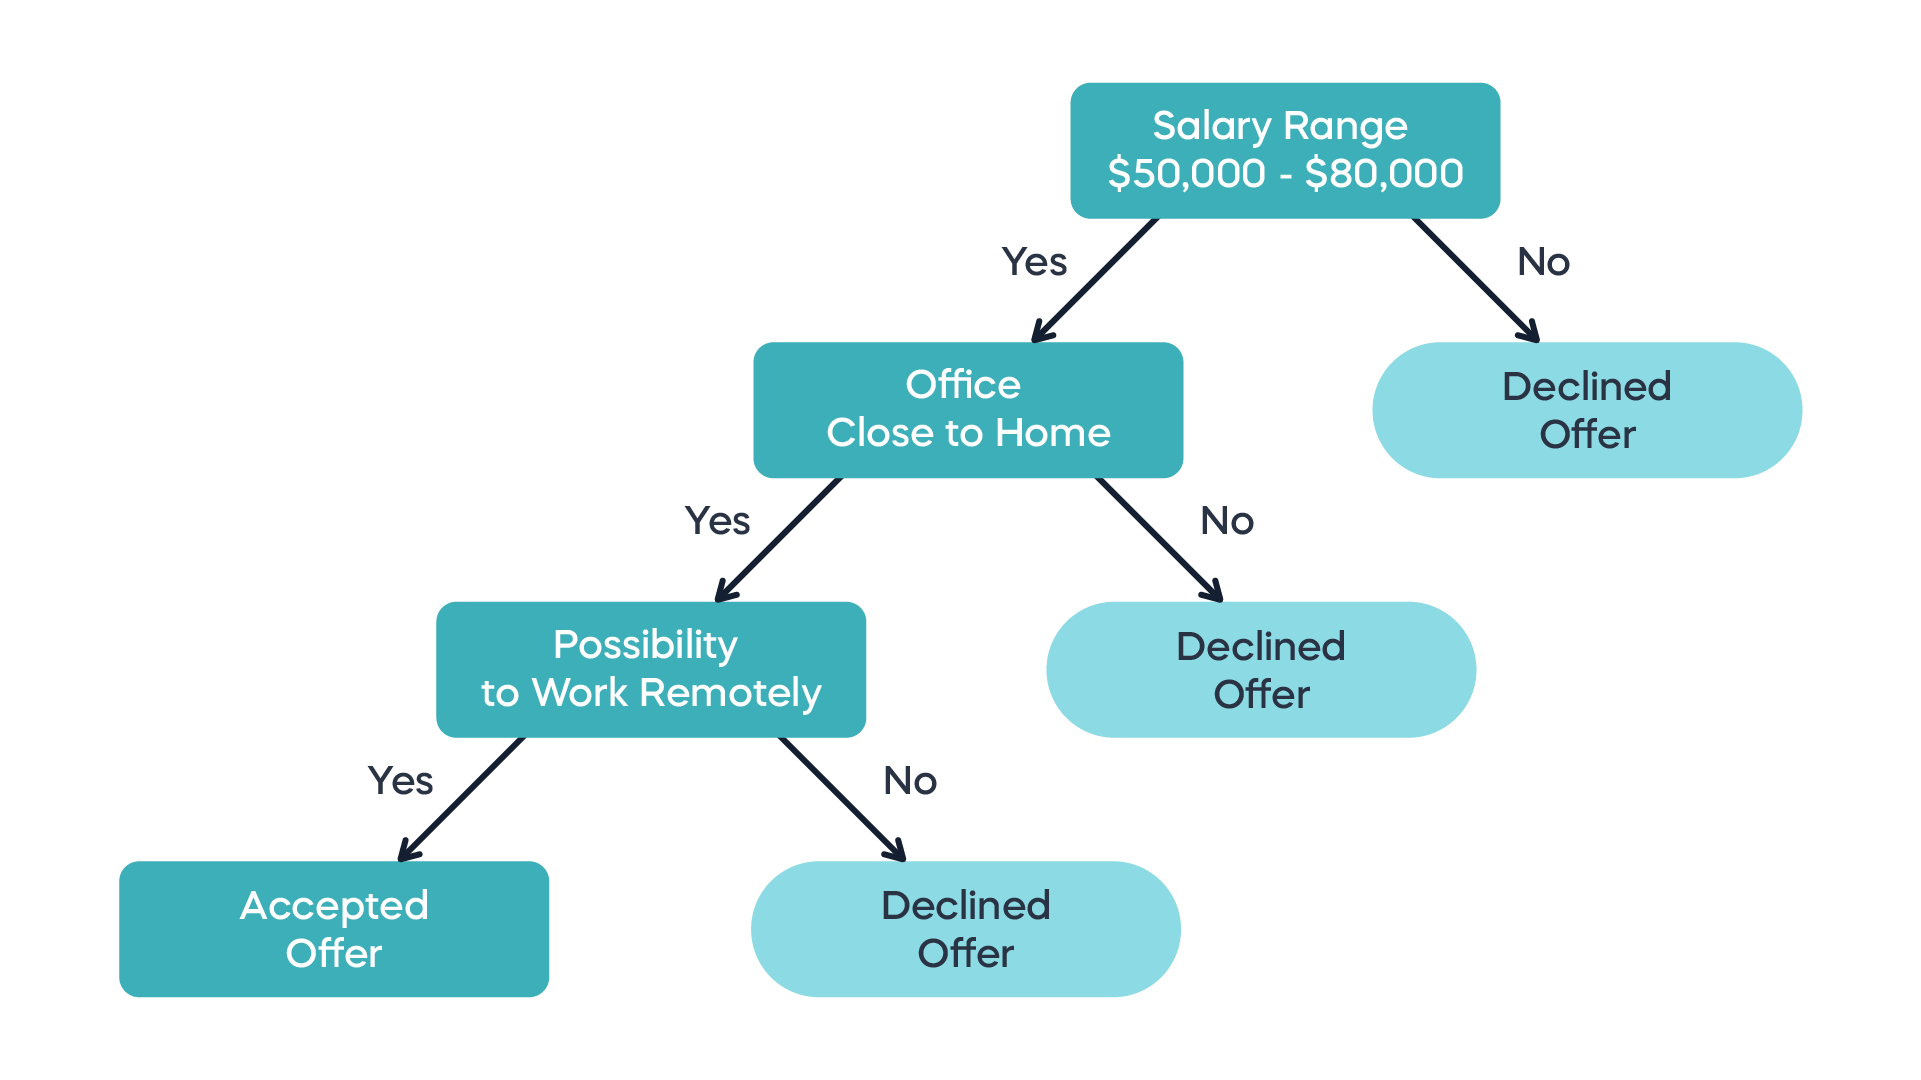
\includegraphics[keepaspectratio]{images/59utffqewug-decision-trees-image2.png}}

}

\caption{Should you take this job? (from
https://365datascience.com/tutorials/machine-learning-tutorials/decision-trees)}

\end{figure}%

Building a decision tree for classification happens by sequential
splitting the space of observations, starting with the decision that
gives the most bang for the buck. Let us define the quality of the split
into \(M\) region by calculating how many observations in that regions
actually belong to each category \(k\). The \emph{Gini index} (or
impurity) is defined as the product of the probability of an observation
(in practice, the fraction of observations in the training set) being
labeled correctly with label \(k\) (\(p_k\)) times the probability of it
being labeled incorrectly (\(1-p_k\)), summed over all the labels \(k\):

\[
G = \sum_k (1-p_k)p_k
\]

Alternatively, one can use the Shannon information or entropy measure:

\[
S = -\sum_k p_k log(p_k)
\]

Notice that both measures are smallest when \(p_k\) is close to 1 or 0,
so they both tell the same story for a particular region: if (almost)
all the points are points are either classified or incorrectly, these
measures are close to 0.

\begin{figure}[H]

{\centering \pandocbounded{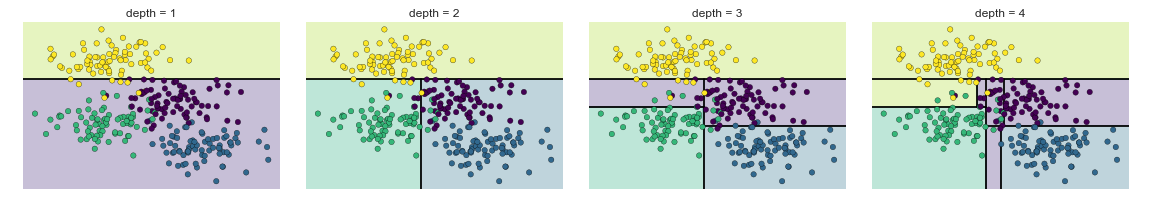
\includegraphics[keepaspectratio]{images/05.08-decision-tree-levels.png}}

}

\caption{Recursive splitting of a two-dimensional set of observations
(from https://jakevdp.github.io/PythonDataScienceHandbook/)}

\end{figure}%

One of these measures is used to create the sequential splits in the
training data set. The biggest problem with this decision tree method is
that it's a greedy algorithm that easily leads to overfitting: as you
can see in the figure above, it can create really complicated regions in
the observation space that may not correspond to meaningful
distinctions.

\subsection{Penguin data}\label{penguin-data}

Define the model specifications for decision trees:

\begin{Shaded}
\begin{Highlighting}[]
\NormalTok{tree\_spec \textless{}{-} decision\_tree() |\textgreater{}}
\NormalTok{  set\_engine("rpart") |\textgreater{}}
\NormalTok{  set\_mode("classification")}
\end{Highlighting}
\end{Shaded}

Create a recipe, apply the model and fit it on the training set:

\begin{Shaded}
\begin{Highlighting}[]
\NormalTok{pen\_recipe \textless{}{-} }
\NormalTok{  recipe(species \textasciitilde{} ., data = pen\_train) |\textgreater{} }
\NormalTok{  update\_role(island,  new\_role = "ID")}

\NormalTok{pen\_workflow\_tree \textless{}{-} workflow() |\textgreater{}}
\NormalTok{  add\_model(tree\_spec) |\textgreater{}}
\NormalTok{  add\_recipe(pen\_recipe)}

\NormalTok{fit\_tree \textless{}{-} pen\_workflow\_tree |\textgreater{} fit(pen\_train)}
\end{Highlighting}
\end{Shaded}

Predict the classification for the test set and validate the
predictions:

\begin{Shaded}
\begin{Highlighting}[]
\NormalTok{compare\_pred \textless{}{-} augment(fit\_tree, new\_data = pen\_test) }

\NormalTok{compare\_pred |\textgreater{} conf\_mat(truth = species, estimate = .pred\_class)}

\NormalTok{compare\_pred |\textgreater{}  accuracy(truth = species, estimate = .pred\_class)}
\end{Highlighting}
\end{Shaded}

Make a plot of the best-fit decision tree:

\begin{Shaded}
\begin{Highlighting}[]
\NormalTok{fit\_tree |\textgreater{}}
\NormalTok{  extract\_fit\_engine() |\textgreater{}}
\NormalTok{  rpart.plot()}
\end{Highlighting}
\end{Shaded}

\subsection{Breast cancer data}\label{breast-cancer-data-1}

Using the same model \texttt{tree\_spec}, create a recipe, apply the
model and fit it on the training set:

\begin{Shaded}
\begin{Highlighting}[]
\NormalTok{can\_recipe \textless{}{-} }
\NormalTok{  recipe(Class \textasciitilde{} ., data = can\_train) |\textgreater{} }
\NormalTok{  update\_role(\textasciigrave{}Uniformity of Cell Shape\textasciigrave{},  \textasciigrave{}Uniformity of Cell Size\textasciigrave{}, \textasciigrave{}Bland Chromatin\textasciigrave{}, new\_role = "ID")}
  

\NormalTok{can\_workflow\_tree \textless{}{-} workflow() |\textgreater{}}
\NormalTok{  add\_model(tree\_spec) |\textgreater{}}
\NormalTok{  add\_recipe(can\_recipe)}

\NormalTok{fit\_tree \textless{}{-} can\_workflow\_tree |\textgreater{} fit(can\_train)}
\end{Highlighting}
\end{Shaded}

Predict the classification for the test set and validate the
predictions:

\begin{Shaded}
\begin{Highlighting}[]
\NormalTok{compare\_pred \textless{}{-} augment(fit\_tree, new\_data = can\_test) }

\NormalTok{compare\_pred |\textgreater{} conf\_mat(truth = Class, estimate = .pred\_class)}

\NormalTok{compare\_pred |\textgreater{}  accuracy(truth = Class, estimate = .pred\_class)}
\end{Highlighting}
\end{Shaded}

Make a plot of the best-fit decision tree:

\begin{Shaded}
\begin{Highlighting}[]
\NormalTok{fit\_tree |\textgreater{}}
\NormalTok{  extract\_fit\_engine() |\textgreater{}}
\NormalTok{  rpart.plot()}
\end{Highlighting}
\end{Shaded}

\section{Random Forests}\label{random-forests}

Overfitting usually results from modeling meaningless noise in the data
instead of real differences. This gave rise to the idea to ``shake up''
the algorithm and see if the splits it produces are robust if the
training set is different. In fact, let's use multiple trees and look at
what the consensus of the \emph{ensemble} can produce. This approach is
called \emph{bagging}, which makes use of an random ensemble of parallel
classifiers, each of which over-fits the data, it combines the results
to find a better classification. An ensemble of randomized decision
trees is known as a \emph{random forest}.

Essentially, the process is as follows: use random sampling from the
data set (bootstrapping) to generate different training sets and train
different decision trees on each. Then for each observation, find its
consensus classification among the whole ensemble; that is, how does the
plurality of the trees classify it.

Since each data point is left out of a number of trees, one can estimate
an unbiased error of classification by computing the ``out-of-bag''
error: for each observation, used the classification produced by all the
trees that did not have this one points in the bag. This is basically a
built-in cross-validation measure.

\subsection{Penguin data}\label{penguin-data-1}

Define the model specification for random forests:

\begin{Shaded}
\begin{Highlighting}[]
\NormalTok{rf\_spec \textless{}{-} rand\_forest(mtry = 4) |\textgreater{}}
\NormalTok{  set\_engine("ranger") |\textgreater{}}
\NormalTok{  set\_mode("classification")}
\end{Highlighting}
\end{Shaded}

Create a recipe, apply the model and fit it on the training set:

\begin{Shaded}
\begin{Highlighting}[]
\NormalTok{rf\_recipe \textless{}{-} }
\NormalTok{  recipe(species \textasciitilde{} ., data = pen\_clean) |\textgreater{} }
\NormalTok{  update\_role(island,  new\_role = "ID")}

\NormalTok{pen\_workflow\_rf \textless{}{-} workflow() |\textgreater{}}
\NormalTok{  add\_model(rf\_spec) |\textgreater{}}
\NormalTok{  add\_recipe(pen\_recipe)}

\NormalTok{fit\_rf \textless{}{-} pen\_workflow\_rf |\textgreater{} fit(pen\_clean)}
\end{Highlighting}
\end{Shaded}

Predict the classification for the test set and validate the
predictions:

\begin{Shaded}
\begin{Highlighting}[]
\NormalTok{compare\_pred \textless{}{-} augment(fit\_rf, new\_data = pen\_clean) }

\NormalTok{compare\_pred |\textgreater{} conf\_mat(truth = species, estimate = .pred\_class)}

\NormalTok{compare\_pred |\textgreater{}  accuracy(truth = species, estimate = .pred\_class)}
\end{Highlighting}
\end{Shaded}

Calculate the ``last fit'' of the entire data set:

\begin{Shaded}
\begin{Highlighting}[]
\NormalTok{last\_rf \textless{}{-} }
\NormalTok{  rand\_forest(mtry = 4, trees = 100) |\textgreater{} }
\NormalTok{  set\_engine("ranger",  importance = "impurity") |\textgreater{} }
\NormalTok{  set\_mode("classification")}
\NormalTok{\# the last workflow}
\NormalTok{last\_workflow \textless{}{-} }
\NormalTok{  pen\_workflow\_rf |\textgreater{} }
\NormalTok{  update\_model(last\_rf)}

\NormalTok{\# the last fit}
\NormalTok{set.seed(3)}
\NormalTok{last\_rf\_fit \textless{}{-} }
\NormalTok{  last\_workflow |\textgreater{} }
\NormalTok{  last\_fit(pen\_split)}
\end{Highlighting}
\end{Shaded}

Plot the importance measures of different variables:

\begin{Shaded}
\begin{Highlighting}[]

\NormalTok{last\_rf\_fit |\textgreater{} }
\NormalTok{  collect\_metrics()}

\NormalTok{last\_rf\_fit |\textgreater{} }
\NormalTok{  pluck(".workflow", 1) |\textgreater{}   }
\NormalTok{  pull\_workflow\_fit() |\textgreater{} }
\NormalTok{  vip(num\_features = 20)}
\end{Highlighting}
\end{Shaded}

\subsection{Cancer data}\label{cancer-data}

Using the same model \texttt{rf\_spec}, create a recipe, apply the model
and fit it on the training set:

\begin{Shaded}
\begin{Highlighting}[]
\NormalTok{can\_rf\_recipe \textless{}{-} }
\NormalTok{  recipe(Class \textasciitilde{} ., data = cancer\_clean) }

\NormalTok{can\_workflow\_rf \textless{}{-} workflow() |\textgreater{}}
\NormalTok{  add\_model(rf\_spec) |\textgreater{}}
\NormalTok{  add\_recipe(can\_rf\_recipe)}

\NormalTok{fit\_rf \textless{}{-} can\_workflow\_rf  |\textgreater{} }
\NormalTok{  fit(cancer\_clean)}
\end{Highlighting}
\end{Shaded}

Predict the classification for the test set and validate the
predictions:

\begin{Shaded}
\begin{Highlighting}[]
\NormalTok{compare\_pred \textless{}{-} augment(fit\_rf, new\_data = can\_test) }

\NormalTok{compare\_pred |\textgreater{} conf\_mat(truth = Class, estimate = .pred\_class)}

\NormalTok{compare\_pred |\textgreater{}  accuracy(truth = Class, estimate = .pred\_class)}
\end{Highlighting}
\end{Shaded}

Calculate the ``last fit'' of the entire data set:

\begin{Shaded}
\begin{Highlighting}[]
\NormalTok{last\_rf \textless{}{-} }
\NormalTok{  rand\_forest(mtry = 4, trees = 100) |\textgreater{} }
\NormalTok{  set\_engine("ranger",  importance = "impurity") |\textgreater{} }
\NormalTok{  set\_mode("classification")}
\NormalTok{\# the last workflow}
\NormalTok{last\_workflow \textless{}{-} }
\NormalTok{  can\_workflow\_rf |\textgreater{} }
\NormalTok{  update\_model(last\_rf)}

\NormalTok{\# the last fit}
\NormalTok{set.seed(3)}
\NormalTok{last\_rf\_fit \textless{}{-} }
\NormalTok{  last\_workflow |\textgreater{} }
\NormalTok{  last\_fit(can\_split)}
\end{Highlighting}
\end{Shaded}

Plot the importance measures of different variables:

\begin{Shaded}
\begin{Highlighting}[]

\NormalTok{last\_rf\_fit |\textgreater{} }
\NormalTok{  collect\_metrics()}

\NormalTok{last\_rf\_fit |\textgreater{} }
\NormalTok{  pluck(".workflow", 1) |\textgreater{}   }
\NormalTok{  pull\_workflow\_fit() |\textgreater{} }
\NormalTok{  vip(num\_features = 20)}
\end{Highlighting}
\end{Shaded}

\section{References}\label{references-2}

\begin{enumerate}
\def\labelenumi{\arabic{enumi}.}
\item
  \href{https://www.statlearning.com/}{Introduction to Statistical
  Learning}
\item
  \href{https://emilhvitfeldt.github.io/ISLR-tidymodels-labs/}{Introcution
  to Statistical Learning Labs with Tidymodels}
\item
  \href{https://www.tidymodels.org/start/case-study/}{Tidy models
  tutorial}
\item
  \href{https://dataaspirant.com/how-decision-tree-algorithm-works/}{How
  Decision Trees Work}
\item
  \href{https://jakevdp.github.io/PythonDataScienceHandbook/05.08-random-forests.html}{Python
  Data Science Handbook}
\item
  \href{https://towardsdatascience.com/rfviz-an-interactive-visualization-package-for-random-forests-in-r-8fb71709c8bf}{Visualization
  of Random Forests}
\end{enumerate}

\bookmarksetup{startatroot}

\chapter{Monte Carlo methods}\label{monte-carlo-methods}

\begin{quote}
\emph{The Monte Carlo casino refused to admit me until I was properly
dressed so I went and found my stockings, and then came back and lost my
shirt.}

--- Dorothy Parker
\end{quote}

\section{Idea}\label{idea}

In statistics, Monte Carlo methods are computational methods in which
repeated, random sampling is used for estimation or hypothesis testing.

They are often used when:

\begin{itemize}
\tightlist
\item
  We have small data sizes, and thus (asymptotic) convergence to known
  distribution is not known.
\item
  We want to apply a permutation test, but there are too many
  permutations.
\item
  Build posterior distributions from Bayesian calculations.
\item
  Determine confidence intervals for parameters that are difficult to
  calculate.
\item
  Test hypotheses on data that are not distributed according to
  convenient, well-studied distributions.
\item
  etc.
\end{itemize}

\section{History}\label{history}

Though examples of what we would call today Monte Carlo methods can be
dated back centuries, the idea was formalized by scientists working on
the Manhattan Project, and especially Stanislaw Ulam (the inventor of
MCMC; the program \texttt{stan} is named after him), Johnny Von Neumann
and Nicholas Metropolis (who came up with the name \emph{Monte Carlo}, a
reference to the famous casino).

These methods have found applications in all the sciences, and beyond.

\section{Bootstrapping}\label{bootstrapping}

The idea is to build confidence intervals for (complex) metrics by
repeatedly re-sampling the data (with replacement), thereby mimicking
the sampling process. This method was pioneered by Bradley Efron
(``Bootstrap Methods: Another Look at the Jackknife'' \emph{Ann.
Statist.} 1979).

The basic algorithm is as follows:

\begin{itemize}
\tightlist
\item
  We have a data set of size \(n\), and we want to compute a certain
  metric on the data.
\item
  We iteratively re-sample the data (with repetition), each time
  obtaining a sample of size \(n\)
\item
  We compute the metric for the re-sampled data sets, thus building a
  distribution for the metric.
\item
  We can compute statistics on the distribution (e.g., percentiles,
  confidence intervals, etc.)
\end{itemize}

\subsection{Example 1}\label{example-1}

We are going to use data on number of bears found per quadrat, found in
a small island in Foxe Basin, Canada, which is occupied by a high
density of bears during the summer ice-free season. The data, collected
using satellite imagery, is taken from Stapleton S. et al.~(``Polar
Bears from Space: Assessing Satellite Imagery as a Tool to Track Arctic
Wildlife'' \emph{PLoS ONE} 2014), and the analysis follows the
presentation in Fieberg, J.D. et al.~(``Resampling-based methods for
biologists'' \emph{PeerJ} 2020).

Let's load the data:

\begin{Shaded}
\begin{Highlighting}[]
\NormalTok{bears \textless{}{-} read.csv("https://raw.githubusercontent.com/StefanoAllesina/BIOS\_26318/refs/heads/master/data/bears.csv")}
\NormalTok{num\_bears \textless{}{-} bears$Num.Bears}
\end{Highlighting}
\end{Shaded}

and compute the mean number of bears per quadrat

\begin{Shaded}
\begin{Highlighting}[]
\NormalTok{mean(num\_bears)}
\end{Highlighting}
\end{Shaded}

and count the number of quadrats

\begin{Shaded}
\begin{Highlighting}[]
\NormalTok{length(num\_bears)}
\end{Highlighting}
\end{Shaded}

What should we expect for the mean if we had access to only 75 quadrats?
We can bootstrap the data? we can approach this by repeatedly sampling
75 quadrats out of the 164 and measure the distribution of the means:

\begin{Shaded}
\begin{Highlighting}[]
\NormalTok{sample\_means \textless{}{-} replicate(1000, mean(sample(num\_bears, 75)))}
\NormalTok{\# this is the average of the sampled means}
\NormalTok{mean(sample\_means)}
\NormalTok{\# typically, confidence intervals are taken to be +/{-} 2 * sd/sqrt(n)}
\NormalTok{confidence \textless{}{-} mean(sample\_means) + c({-}2, 2) * sd(sample\_means)/sqrt(75)}
\NormalTok{confidence}
\end{Highlighting}
\end{Shaded}

\section{Example 2}\label{example-2}

Another example, taken from Fieberg et al.

\begin{quote}
{[}Consider the{]} data collected by the Minnesota Department of Natural
Resources to explore the potential impact of changing fishing
regulations on the size distribution of northern pike (Esox lucius) in
Medicine Lake, an approximately 460-acre lake in Beltrami County, MN. In
1989, the MN DNR instituted a slot limit of 22--30 inches in this lake
(i.e., all caught fish within this size interval had to be released). We
consider length data from 73 and 81 fish collected in trap nets in 1988
and 1993, respectively (before and after the fishing regulation was put
in place). Importantly, these data come from only one lake, and many
other factors may have changed between 1988 and 1993. Therefore, we must
be cautious when interpreting any changes in the distribution of fish
sizes (i.e., attributing the cause of length changes to the management
regulation or generalizing results to other lakes). Nonetheless, we can
ask, ``How much did fish length, on average, change between 1988 and
1993 in Medicine Lake?'' To address this question, we estimate the
difference in the mean length of fish in the two samples. We also
quantify our uncertainty in this estimated difference in means,
recognizing that we would get a different estimate if we could go back
and collect other samples of fish in those 2 years.
\end{quote}

Let's read the data

\begin{Shaded}
\begin{Highlighting}[]
\NormalTok{dt \textless{}{-} read.csv("https://raw.githubusercontent.com/StefanoAllesina/BIOS\_26318/refs/heads/master/data/Pikedata.csv")}
\end{Highlighting}
\end{Shaded}

And divide it by year

\begin{Shaded}
\begin{Highlighting}[]
\NormalTok{y1988 \textless{}{-} dt$length.inches[dt$year == 1988]}
\NormalTok{y1993 \textless{}{-} dt$length.inches[dt$year == 1993]}
\NormalTok{print(mean(y1993) {-} mean(y1988))}
\end{Highlighting}
\end{Shaded}

Showing that fish in 1993 were 2.6 inches longer. Because we caught a
small number of fish (about 80) per year, we can build a distribution
for the difference by bootstrapping

\begin{Shaded}
\begin{Highlighting}[]
\NormalTok{sample\_mean \textless{}{-} function(x)\{}
\NormalTok{  mean(sample(x, length(x), replace = TRUE))}
\NormalTok{\}}

\NormalTok{diff\_sample \textless{}{-} replicate(1000, sample\_mean(y1993) {-} sample\_mean(y1988))}
\NormalTok{hist(diff\_sample)}
\NormalTok{abline(v = mean(y1993) {-} mean(y1988))}
\end{Highlighting}
\end{Shaded}

\section{Hypothesis testing using Monte
Carlo}\label{hypothesis-testing-using-monte-carlo}

These methods are often used when we can easily sample from the null
model (i.e., a model encoding the null hypothesis), and we want to
compute some statistics on the observed data v. the randomized data. We
can associate an ``empirical'' p-value to the test, by measuring how
often the statistics on the randomized data exceeds that measured for
the empirical data.

\subsection{Example: penguin breeding
pairs}\label{example-penguin-breeding-pairs}

This example is taken from Graeme Ruxton \& Markus Neuhäuser
(``Improving the reporting of P-values generated by randomization
methods'', \emph{Methods in Eco \& Evol} 2013).

\begin{quote}
Massaro \& Blair (\emph{New Zealand J. Ecol}, 2003) wanted to compare
the numbers of breeding yellow-eyed penguins (\emph{Megadyptes
antipodes}) on Stewart Island off New Zealand with those on nearby
islands, which (unlike Stewart Island) had no feral cats (\emph{Felis
catus}) that are potential predators of the penguins. They visited 19
breeding colonies on Stewart island and recorded the following numbers
of breeding pairs at them \{7,3,3,7,3,7,3,10,1,7,4,1,3,2,1,2,9,4,2\},
and 10 colonies on nearby islands where the recorded numbers of pairs
were \{15,32,1,13,14,11,1,3,2,7\}. Thus, in total, 178 breeding pairs
were observed; on Stewart Island, the mean colony size (±SE) was 4.2
(±0.6), whereas on other islands, it was 9.9 (±3). We want to explore by
randomization whether this sample gives reason for rejecting the null
hypothesis that each pair chooses a breeding site (independently)
without regard to the presence of cats. {[}\ldots{]} Given the
noticeably lower variability among colony sizes on Stewart Island, an
appropriate test statistic to adopt might be the \emph{t} statistic for
samples with unequal variance (Ruxton 2006). For each randomization,
each of the 178 pairs independently chooses one of the 29 colonies (each
with equal probability).
\end{quote}

In a nutshell, the idea is to

\begin{enumerate}
\def\labelenumi{\arabic{enumi}.}
\tightlist
\item
  measure the t statistics for the observed data
\item
  repeatedly generate randomized data by assigning the 178 pairs to the
  colonies at random
\item
  measure the t statistics for the randomized data, forming a
  distribution
\item
  compute the (empirical) probability of finding a value for the
  randomized data that is larger than that found for the observed data
\end{enumerate}

\begin{Shaded}
\begin{Highlighting}[]
\NormalTok{set.seed(1)}
\NormalTok{original \textless{}{-} c(c(7,3,3,7,3,7,3,10,1,7,4,1,3,2,1,2,9,4,2), \# Stewart Island}
\NormalTok{              c(15,32,1,13,14,11,1,3,2,7) \# other island}
\NormalTok{              )}
\NormalTok{\# compute t{-}stat for original data [first 19 are one island, the rest are the other island]}
\NormalTok{tobs \textless{}{-} abs(t.test(original[1:19], original[{-}(1:19)])$statistic)}
\NormalTok{\# now randomized the data and record the number of times we\textquotesingle{}ve found a value larger than the }
\NormalTok{\# one observed for the empirical data}
\NormalTok{num\_rand \textless{}{-} 999}
\NormalTok{p\_value \textless{}{-} 0}
\NormalTok{for (i in 1:num\_rand)\{}
\NormalTok{  randomized \textless{}{-} table(sample(1:29, 178, replace = TRUE))}
\NormalTok{  trnd \textless{}{-} abs(t.test(randomized[1:19], randomized[{-}(1:19)])$statistic)}
\NormalTok{  if (trnd \textgreater{}= tobs) p\_value \textless{}{-} p\_value + 1}
\NormalTok{\}}
\NormalTok{print(p\_value)}
\end{Highlighting}
\end{Shaded}

In this case, we have observed a larger (or equal) value 61 times out of
999 randomizations. The last step is to divide this number by the number
of simulations, to obtain a probability. There are two ways to do this:

\[
p = \frac{\sum_i{I(x_i \geq X})}{n}
\]

where \(x_i\) is the statistics for randomization \(i\), \(X\) is the
statistics for the observed data, and \(n\) is the number of
randomizations. In this case:

\begin{Shaded}
\begin{Highlighting}[]
\NormalTok{p\_value / 999}
\end{Highlighting}
\end{Shaded}

Alternatively, and slightly more conservatively, we can assume that the
empirical data was also sampled from the null model, in which case:

\[
p = \frac{1+ \sum_i{I(x_i \geq X})}{n + 1}
\]

yielding:

\begin{Shaded}
\begin{Highlighting}[]
\NormalTok{(1 + p\_value) / 1000}
\end{Highlighting}
\end{Shaded}

The difference between the two approaches is largest when the
probability of observing a large value in the randomizations is very
small (in one case we would get \(0\), in the other \(1/(n+1)\)). Ruxton
\& Neuhäuser recommend stating the choice explicitly, to improve
replicability. A discussion of this issue in the field of genetics can
be found in North \emph{et al.} (``A Note on the Calculation of
Empirical P Values from Monte Carlo Procedures'', \emph{Am J Hum Genet}
2002); Gandy (``Sequential implementation of Monte Carlo Tests with
uniformly bounded resampling risk'' \emph{Journal of the American
Statistical Association} 2000) provides an algorithm to compute
confidence intervals on the empirical p-value.

Naturally, the larger the number of simulations, the more accurate the
result. The rule of thumb is that one would need about \(10^4\)
randomizations to be confident in the first two decimals.

\section{Randomizing binary tables (bipartite
networks)}\label{randomizing-binary-tables-bipartite-networks}

Often, biological data is represented by binary, rectangular tables. For
example:

\begin{itemize}
\tightlist
\item
  Rows are sampling sites, and columns are species; a 1 marks the
  presence of a species at a site, and a 0 its absence.
\item
  Rows are individuals and columns are SNPs.
\item
  Rows are species and columns are traits.
\item
  Rows are genes and columns are times; a 1 marks genes that are
  significantly over-expressed at a given time.
\item
  \ldots{}
\end{itemize}

These data can be represented as either a binary, rectangular matrix, or
equivalently as a bipartite network.

One of the most salient feature of such a table is given by its marginal
totals (row/col sums, or the degree of the nodes in the bipartite
network). The marginal totals/degrees greatly influence the
network/table structure. For example, in extreme cases there is only one
binary table/network with a given set of degrees.

\begin{Shaded}
\begin{Highlighting}[]
\NormalTok{A \textless{}{-} matrix(c(}
\NormalTok{  1,1,1,1,}
\NormalTok{  1,1,1,0,}
\NormalTok{  1,1,1,0,}
\NormalTok{  1,1,0,0,}
\NormalTok{  1,0,0,0}
\NormalTok{), 5, 4, byrow = TRUE)}
\NormalTok{B \textless{}{-} matrix(c(}
\NormalTok{  1,1,1,1,}
\NormalTok{  1,1,1,0,}
\NormalTok{  1,1,0,1,}
\NormalTok{  1,1,0,0,}
\NormalTok{  1,0,0,0}
\NormalTok{), 5, 4, byrow = TRUE)}
\NormalTok{A}
\NormalTok{B}
\end{Highlighting}
\end{Shaded}

\subsection{Randomizing the network: checkerboard
swapping}\label{randomizing-the-network-checkerboard-swapping}

If we can identify two rows and two columns such that the induced
submatrix is

\begin{longtable}[]{@{}lll@{}}
\toprule\noalign{}
& a & b \\
\midrule\noalign{}
\endhead
\bottomrule\noalign{}
\endlastfoot
A & 0 & 1 \\
B & 1 & 0 \\
\end{longtable}

or

\begin{longtable}[]{@{}lll@{}}
\toprule\noalign{}
& a & b \\
\midrule\noalign{}
\endhead
\bottomrule\noalign{}
\endlastfoot
A & 1 & 0 \\
B & 0 & 1 \\
\end{longtable}

we can swap the submatrix for the other, without altering the row/col
marginal totals.

\subsection{Randomizing the network:
curveball}\label{randomizing-the-network-curveball}

The same idea can be generalized. One fun way to think about this,
introduced by Strona et al.~(``A fast and unbiased procedure to
randomize ecological binary matrices with fixed row and column totals''
\emph{Nature Comm} 2014) is to consider children exchanging baseball
cards. In the example above, the cards are the columns and the children
are the rows, and two children exchange one card (for example, A does
not have card b, and B does not have card a; if they exchange them the
number of cards per child and the number of children per card are
unchanged).

Take two rows of a binary matrix:

\begin{longtable}[]{@{}llllllll@{}}
\toprule\noalign{}
& a & b & c & d & e & f & g \\
\midrule\noalign{}
\endhead
\bottomrule\noalign{}
\endlastfoot
A & 0 & 1 & 0 & 1 & 1 & 1 & 0 \\
B & 1 & 1 & 1 & 0 & 1 & 0 & 1 \\
\end{longtable}

The intersection set \(A \cap B\) is given by \{a,c,d,f,g\}, with A
contributing two ``cards'' (d, f) and B contributing three (a,c,g). If
we pool all the cards in the intersection, and then A picks two at
random, and B the remaining three, the marginals are unchanged.

Clearly, the ``mixing'' of the table is faster, because we can trade
several cards at once. It can be proven that, after a sufficiently large
number of trades, the resulting table/network is sampled uniformly from
the set of tables/networks with the given marginal totals.

For example, create a random binary table, and shuffle it keeping the
marginal totals:

\begin{Shaded}
\begin{Highlighting}[]
\NormalTok{set.seed(1)}
\NormalTok{source("https://raw.githubusercontent.com/StefanoAllesina/BIOS\_26318/refs/heads/master/data/curveball.R")}
\NormalTok{\# create a random table}
\NormalTok{A \textless{}{-} matrix((runif(10 * 7) \textless{} 0.5) * 1, 10, 7)}
\NormalTok{\# this are the the marginal totals}
\NormalTok{rowSums(A)}
\NormalTok{colSums(A)}
\NormalTok{\# randomize the matrix}
\NormalTok{B \textless{}{-} curveball.run(A, 1000)}
\end{Highlighting}
\end{Shaded}

\subsection{Example: Darwin's finches}\label{example-darwins-finches}

Jared Diamond proposed that the presence/absence of species on islands
would be influenced by competition: bird species would try avoiding
overlapping with their competitors, and would tend to co-occur with
species they are not competing with. While this idea generated a very
contentious debate, here we are going to test this hypothesis using the
famous Darwin's finches (see Weiner, \emph{The Beak of the Finch: A
Story of Evolution in Our Time} 1994), using a metric proposed by
Roberts and Stone. Take \(A\) to be a matrix with the \(m\) finch
species as rows, and \(n\) islands as columns; a 1 marks the presence of
a finch species on an island. The matrix \(S = A A^T\) counts the number
of islands in which species co-occur. Naturally, the diagonal reports
the number of islands in which a finch species is found.

Roberts and Stone proposed to measure:

\[
\bar{S^2} = \frac{1}{m (m-1)} \sum_{i\neq j}S_{ij}^2
\]

This number is small if finch species do not co-occurr often, and is
high when some species always co-occur. We are going to use the
curveball algorithm to randomize the species data, and then compute an
empirical p value for the probability of observing this result by
chance:

\begin{Shaded}
\begin{Highlighting}[]
\NormalTok{finches \textless{}{-} as.matrix(read.csv("https://raw.githubusercontent.com/StefanoAllesina/BIOS\_26318/refs/heads/master/data/finches.csv"))}
\NormalTok{\# compute mean squared overlap, excluding self}
\NormalTok{\# index proposed by Roberts and Stone, Oecologia 1990}
\NormalTok{mean\_sq\_ol \textless{}{-} function(M)\{}
\NormalTok{  M2 \textless{}{-} (M) \%*\% t(M) \# number of co{-}occurrences}
\NormalTok{  diag(M2) \textless{}{-} NA \# no self}
\NormalTok{  return(mean(M2\^{}2, na.rm = TRUE))}
\NormalTok{\}}
\NormalTok{\# observed value}
\NormalTok{obs \textless{}{-} mean\_sq\_ol(finches)}
\NormalTok{\# randomizations}
\NormalTok{nrand \textless{}{-} 249}
\NormalTok{pval \textless{}{-} 0}
\NormalTok{for (i in 1:nrand)\{}
\NormalTok{  tmp \textless{}{-} mean\_sq\_ol(curveball.run(finches, 250))}
\NormalTok{  if (tmp \textgreater{}= obs) \{ \# testing "partitioning/competition" }
\NormalTok{    pval \textless{}{-} pval + 1}
\NormalTok{  \}}
\NormalTok{\}}
\NormalTok{print((pval + 1) / (nrand + 1))}
\end{Highlighting}
\end{Shaded}

we conclude that our null model (finches choose random islands,
considering that some fiches are more widespread than others, and that
some islands harbor a larger number of species) would not generate such
a high value by chance with high probability, and thus we reject the
hypothesis.

\bookmarksetup{startatroot}

\chapter{Time series: modeling and
forecasting}\label{time-series-modeling-and-forecasting}

\begin{Shaded}
\begin{Highlighting}[]
\NormalTok{library(tsibble)}
\NormalTok{library(tsibbledata)}
\NormalTok{library(lubridate)}
\NormalTok{library(fable)}
\NormalTok{library(feasts)}
\NormalTok{\#library(forecast)}
\NormalTok{\#library(fpp2)}
\end{Highlighting}
\end{Shaded}

\begin{quote}
Prediction is difficult, especially about the future.

--- Niels Bohr (apocryphally)
\end{quote}

\section{Goals:}\label{goals}

\begin{itemize}
\tightlist
\item
  Use current tools for handling and visualizing time series
\item
  Calculate auto- and cross-correlations of time series
\item
  Decompose time series into components
\item
  Use linear regression methods for fitting and forecasting
\end{itemize}

\section{Time series format and
plotting}\label{time-series-format-and-plotting}

A time series is a special data set where each observation has an
associated time measurement. There is a special R structure for storing
and operating on time series, called \texttt{ts}, as illustrated here:

\begin{Shaded}
\begin{Highlighting}[]
\NormalTok{births \textless{}{-} scan("https://robjhyndman.com/tsdldata/data/nybirths.dat")}
\NormalTok{birthstimeseries \textless{}{-} ts(births, frequency = 12, start = c(1946, 1))}
\NormalTok{birthstimeseries}
\end{Highlighting}
\end{Shaded}

This reads in a data set recording the number of births per month in New
York City, from 1946 to 1958 (in thousands of births?) To create the
time series, we had to give the function the \texttt{frequency}, or the
number of time points in a year, and the starting value as a vector
assigned to \texttt{start\ =\ c(1946,\ 1)}, the first element is the
year and the second the month.

There are several other specialized data structures for handling time
series. We will use one from a new set of R packages called
\texttt{tidyverts} that is called a \texttt{tsibble}.
https://tsibble.tidyverts.org/ The \texttt{tsibbledata} package contains
several time series data sets and we will load two below:
\texttt{olympic\_running}, containing the Olympic winning times in
different running events, and \texttt{pelt}, containing the classic data
of the number of Lynx and Hare pelts sold in Canada in the 19th and
early 20th centuries:

\begin{Shaded}
\begin{Highlighting}[]
\NormalTok{data("olympic\_running")}
\NormalTok{glimpse(olympic\_running)}
\NormalTok{data("pelt")}
\NormalTok{glimpse(pelt)}
\end{Highlighting}
\end{Shaded}

You can see that tsibbles contain multiple variables, one of which is
the time variable and is called the index, and one or more others are
denoted as key, which are variables that identify the observations but
are not changing in time. For example, in the Olympic times data set,
the Sex and the Length are the keys, because they are not measurement
that we're plotting over time. In the pelt data set, there is no key
variable (but you could make a longer tsibble with species as the key
variable if you wanted.)

\subsection{Visualizing the data}\label{visualizing-the-data}

The most straightforward way of visualizing time series is using a time
plot, which can be created using \texttt{autoplot}:

\begin{Shaded}
\begin{Highlighting}[]
\NormalTok{autoplot(birthstimeseries) +}
\NormalTok{  ggtitle("Number of births in NYC") +}
\NormalTok{  ylab("Births (thousands)") +}
\NormalTok{  xlab("Year")}
\end{Highlighting}
\end{Shaded}

\texttt{autoplot} works best with timeseries objects, so to use it with
a tsibble you can convert it to a ts first, like this:

\begin{Shaded}
\begin{Highlighting}[]
\NormalTok{autoplot(as.ts(pelt)) +}
\NormalTok{  ggtitle("Lynx and hare pelts") +}
\NormalTok{  ylab("Number of pelts") +}
\NormalTok{  xlab("Year")}
\end{Highlighting}
\end{Shaded}

One can also use \texttt{ggplot} directly, for example to plot a faceted
graph of the olympic times for different years:

\begin{Shaded}
\begin{Highlighting}[]
\NormalTok{olympic\_running |\textgreater{} as\_tibble |\textgreater{}}
\NormalTok{  ggplot(aes(x=Year, y = Time, colour = Sex)) +}
\NormalTok{  geom\_line() +}
\NormalTok{  facet\_wrap(\textasciitilde{} Length, scales = "free\_y")}
\end{Highlighting}
\end{Shaded}

\section{Decomposition of time
series}\label{decomposition-of-time-series}

As you can see from the plots above, time series are often a combination
of different time-dependent processes and it is often useful to think
about them separately. One can distinguish three types of time variation
in time series:

\begin{quote}
\begin{itemize}
\item
  \textbf{Seasonality} A seasonal pattern occurs when a time series is
  affected by seasonal factors such as the time of the year or the day
  of the week. Seasonality is always of a fixed and known frequency.
\item
  \textbf{Trend} A trend exists when there is a long-term increase or
  decrease in the data. It does not have to be linear. Sometimes we will
  refer to a trend as ``changing direction'', when it might go from an
  increasing trend to a decreasing trend.
\item
  \textbf{Cyclic} A cycle occurs when the data exhibit rises and falls
  that are not of a fixed frequency. In economics, these fluctuations
  may by due to economic conditions and are often related to the
  ``business cycle''.
\end{itemize}
\end{quote}

\subsection{Decomposition of time
series}\label{decomposition-of-time-series-1}

There are two main types of decompositions of time series: additive and
multiplicative. Let us call \(X_t\) the time series data, \(T_t\) the
trend (non-periodic component), \(S_t\) the seasonal part (periodic
component), and \(R_t\) the remainder.

\[
X_t = T_t + S_t + R_t
\] \[
X_t = T_t \times S_t \times R_t
\]

One simple way of removing seasonality and estimating the trend is using
the \emph{moving average}, that is using \(k\) points before and \(k\)
points after each point to calculate the trend: \[
T_t =  \frac{1}{m} \sum_{i=-k}^k X_{t+i}
\]

Here \(m\) is called the \emph{order} of the moving average and is
defined as \(m = 2k+1\). There is a useful function \texttt{ma()} that
calculates these averages and allows them to be plotted.

\begin{Shaded}
\begin{Highlighting}[]
\NormalTok{m \textless{}{-} 6}
\NormalTok{s\_name \textless{}{-} paste("MA{-}", m)}
\NormalTok{autoplot(birthstimeseries, series = "data") +}
\NormalTok{  autolayer(ma(birthstimeseries, m), series = "MA") +}
\NormalTok{  xlab("Time (Year)") + ylab("number of births (thousands)") +}
\NormalTok{  ggtitle("NYC births time series") }
\end{Highlighting}
\end{Shaded}

\textbf{Exercise:} Change the moving average window and see if you can
make seasonality (periodicity) vanish!

An even order of periodicity requires an asymmetric averaging window, so
to create an symmetric average, one can repeat the moving average of
order two on the already-averaged data.

\subsection{Classic decomposition:}\label{classic-decomposition}

Additive decomposition {[}1{]}:

\begin{enumerate}
\def\labelenumi{\arabic{enumi}.}
\tightlist
\item
  If m is an even number, compute the trend-cycle component \(T_t\)
  using a 2×m-MA. If m is an odd number, compute the trend-cycle
  component \(\hat T_t\) using an m-MA.
\item
  Calculate the detrended series: \(X_t - \hat T_t\)
\item
  To estimate the seasonal component for each season, average the
  detrended values for that season. For example, with monthly data, the
  seasonal component for March is the average of all the detrended March
  values in the data. These seasonal component values are then adjusted
  to ensure that they add to zero. The seasonal component is obtained by
  stringing together these monthly values, and then replicating the
  sequence for each year of data. This gives \(\hat S_t\).
\item
  The remainder component is calculated by subtracting the estimated
  seasonal and trend-cycle components:
  \(\hat R_t = X_t - \hat T_t - \hat S_t\)
\end{enumerate}

\begin{Shaded}
\begin{Highlighting}[]
\NormalTok{birthstimeseries |\textgreater{} decompose(type="additive") |\textgreater{}}
\NormalTok{  autoplot() + xlab("Year") +}
\NormalTok{  ggtitle("Classic additive decomposition}
\NormalTok{    of the NYC births time series")}
\end{Highlighting}
\end{Shaded}

This simple classical decomposition has numerous flaws, so better, more
modern methods are preferred. In particular, it assumes a constant
seasonal term, it tends to over-estimate the variation in the trend, it
misses data for the first few and last few data points, and can be
sensitive to outliers.

\subsection{STL decomposition}\label{stl-decomposition}

A more robust method is called the STL decomposition (Seasonal and Trend
decomposition using Loess). To summarize its advantages {[}1{]}:

\begin{itemize}
\tightlist
\item
  STL can handle any type of seasonality, not only monthly and quarterly
  data.
\item
  The seasonal component is allowed to change over time, and the rate of
  change can be controlled by the user.
\item
  The smoothness of the trend-cycle can also be controlled by the user.
\item
  It can be robust to outliers (i.e., the user can specify a robust
  decomposition), so that occasional unusual observations will not
  affect the estimates of the trend-cycle and seasonal components. They
  will, however, affect the remainder component.
\end{itemize}

\begin{Shaded}
\begin{Highlighting}[]
\NormalTok{birthstimeseries |\textgreater{}  stl(t.window=13, s.window="periodic", robust=TRUE) |\textgreater{}}
\NormalTok{  autoplot()}
\end{Highlighting}
\end{Shaded}

\textbf{Exercise:} Apply the two decomposition methods to the pelt time
series data.

\section{Relationships within and between time
series}\label{relationships-within-and-between-time-series}

\subsection{Visualizing correlation between different
variables}\label{visualizing-correlation-between-different-variables}

The following data set contains the number of visitors (visitor nights)
on a quarterly basis for five regions of New South Wales, Australia:

\begin{Shaded}
\begin{Highlighting}[]
\NormalTok{autoplot(visnights[,1:5]) +}
\NormalTok{  ylab("Number of visitor nights each quarter (millions)")}
\end{Highlighting}
\end{Shaded}

One simple question is whether different variables are related to each
other. One simple way is to calculate the Pearson correlation between
different time series, called the \emph{cross-correlation} (where
\(\bar X\) stands for the mean of X and \(\text{Var}(X)\) stands for the
variance of \(X\)):

\[
\text{Cor}(X,Y) = \frac{\sum_t (\bar X - X_t)(\bar Y - Y_t)}{\sqrt{\text{Var}(X)\text{Var}(Y)}}
\]

In a data set with multiple variables it can be handy to examine the
cross-correlations between all pairs between them. Here's a convenient
function to both calculate and visualize it for multiple variables, in
this case the hotel visitor nights for the 5 different regions of NSW.
The plot below show the scatter plots of all the pairs of time series
against each other, along with the respective correlation coefficients:

\begin{Shaded}
\begin{Highlighting}[]
\NormalTok{head(visnights)}
\NormalTok{GGally::ggpairs(as.data.frame(visnights[,1:5]))}
\end{Highlighting}
\end{Shaded}

However, sometimes the straightforward correlation may miss or
underestimate a relationship that is obviously there, but with a delay.
Here is the Lynx and Hare variables from the pelts data set correlated
with each other:

\begin{Shaded}
\begin{Highlighting}[]
\NormalTok{head(pelt)}
\NormalTok{GGally::ggpairs(pelt[,2:3])}
\end{Highlighting}
\end{Shaded}

The correlation coefficient is about 0.3, but it appears that the
relationship should be stronger than that from the plots. The function
\texttt{CCF} from \texttt{feasts} package calculates correlations for a
pair of variables that are shifted against each other (lagged) and here
is the resulting plot:

\begin{Shaded}
\begin{Highlighting}[]
\NormalTok{pelt |\textgreater{}}
\NormalTok{  CCF(Lynx, Hare, lag\_max = 8) |\textgreater{}}
\NormalTok{  autoplot()}
\end{Highlighting}
\end{Shaded}

You can see the non-shifted correlation of about 0.3 at lag of 0, but
the correlation is about 2 times higher when the series is shifted by 1
or 2 years, as suggested by the time plots of the series.

\subsection{Autocorrelation}\label{autocorrelation}

Just as we saw for cross-correlations, a time series can be correlated
against itself shifted in time by some set amount, also called
\emph{lagged}. We can plot the lagged correlations for different visitor

\begin{Shaded}
\begin{Highlighting}[]
\NormalTok{visnights[,1]}
\NormalTok{visnights\_smaller \textless{}{-} window(visnights[,2], start=2000, end = 2010)}
\NormalTok{gglagplot(visnights\_smaller) }
\end{Highlighting}
\end{Shaded}

Here the colors indicate the quarter of the variable on the vertical
axis, compared with the shifted (lagged variable on the horizontal axis,
and the lines connect points in chronological order. The relationship is
strongly positive at lags 4 and 8, reflecting the strong seasonality in
the data.

This suggests that there is a strong similarity between the time series
and itself, shifted by certain time values. This is described by the
\emph{autocorrelation}, which is defined as a function of the lag \(k\):

\[
r(k) = \frac{\sum_{t=k}^T (\bar X - X_t)(\bar X - X_{t-k})}{\text{Var}(X)}
\]

The autocorrelation can be calculated and plotted for our example of the
visitation nights in New South Wales:

\begin{Shaded}
\begin{Highlighting}[]
\NormalTok{ggAcf(visnights\_smaller)}
\end{Highlighting}
\end{Shaded}

\begin{Shaded}
\begin{Highlighting}[]
\NormalTok{gglagplot(pelt$Lynx, lags =12) + ggtitle("Lag plots for the Lynx pelt data")}
\NormalTok{gglagplot(pelt$Hare, lags = 12) + ggtitle("Lag plots for the Hare pelt data")}
\end{Highlighting}
\end{Shaded}

In both cases, the lag plots are closest to the diagonal identity line
for lag of 9 or 10. This should be reflected in the autocorrelation
plot:

\begin{Shaded}
\begin{Highlighting}[]
\NormalTok{ggAcf(pelt$Lynx) + ggtitle("Autocorrelation for the Lynx pelt data")}
\NormalTok{ggAcf(pelt$Hare) + ggtitle("Autocorrelation for the Hare pelt data")}
\end{Highlighting}
\end{Shaded}

Notice the periodicity in the autocorrelation, which indicated
periodicity in the time series.

Autocorrelation measures the \emph{memory} of a signal - for example,
pure white noise is uncorrelated with itself even a moment later, and
thus has no memory. As such, it is very useful as a measure of a trend
in the data - if the time series has slowly decaying, positive
autocorrelation, that indicates a pronounced trend, while periodicity
indicates seasonality in the data.

\textbf{Exercise:} Use the lag and autocorrelation analysis to describe
the patterns in the time series of births in NYC.

\subsection{Perennial warning: correlations are not
causation!}\label{perennial-warning-correlations-are-not-causation}

These two data sets, on Australian air passengers and rice production in
Guinea, have a very strong positive correlation:

\begin{Shaded}
\begin{Highlighting}[]
\NormalTok{aussies \textless{}{-} window(ausair, end=2011)}
\NormalTok{fit \textless{}{-} tslm(aussies \textasciitilde{} guinearice)}
\NormalTok{summary(fit)}
\end{Highlighting}
\end{Shaded}

However, notice that the residuals indicate a strong trend, which
violates the assumptions of linear regression.

\begin{Shaded}
\begin{Highlighting}[]
\NormalTok{checkresiduals(fit)}
\end{Highlighting}
\end{Shaded}

There are a number of fun examples of spurious time series correlations
in reference {[}5{]}.

\section{Modeling and forecasting}\label{modeling-and-forecasting}

\subsection{Forecasting using smoothing
methods}\label{forecasting-using-smoothing-methods}

The package \texttt{fable} is part of the \texttt{tidyverts} bundle and
can be used to easily produce forecasts using several standard methods,
such as ASNAIVE (Seasonal Naive), ETS (exponential smoothing), and ARIMA
(AutoRegressive Integrated Moving Average). The code below compares all
three forecast models for the births in NYC data:

\begin{Shaded}
\begin{Highlighting}[]
\NormalTok{as\_tsibble(birthstimeseries) |\textgreater{} }
\NormalTok{  model(}
\NormalTok{    ets = ETS(box\_cox(birthstimeseries, 0.3)),}
\NormalTok{   arima = ARIMA(log(birthstimeseries)),}
\NormalTok{    snaive = SNAIVE(birthstimeseries)}
\NormalTok{  ) |\textgreater{}}
\NormalTok{  forecast(h = "2 years") |\textgreater{} }
\NormalTok{  autoplot(birthstimeseries)}
\end{Highlighting}
\end{Shaded}

\section{References and further
reading:}\label{references-and-further-reading-1}

\begin{enumerate}
\def\labelenumi{\arabic{enumi}.}
\tightlist
\item
  Rob J Hyndman and George Athanasopoulos.
  \href{https://otexts.com/fpp2/}{\textbf{Forecasting: Principles and
  Practice}}
\item
  Jonathan Cryer and Kung-Sik Chan
  \href{https://mybiostats.files.wordpress.com/2015/03/time-series-analysis-with-applications-in-r-cryer-and-chan.pdf}{\textbf{Time
  Series Analysis with Applications in R}}
\item
  \href{https://www.r-bloggers.com/time-series-forecast-cross-validation-by-ellis2013nz/}{Cross-validation
  in forecasting}
\item
  \href{https://towardsdatascience.com/time-series-nested-cross-validation-76adba623eb9}{Time
  series nested cross-validation}
\item
  \href{https://www.tylervigen.com/spurious-correlations}{Spurious
  correlations}
\end{enumerate}




\end{document}
